% !TeX spellcheck = pt_BR

\chapter{Cinemática Vetorial}


\section{Introdução}

Vamos agora adentrar no estudo de movimentos bidimensionais. Até então, por estarmos trabalhando com movimentos em apenas uma dimensão, foi possível deixar de lado o caráter \textbf{vetorial} das grandezas cinemáticas -- e é deles que vamos tratar daqui em diante. Note, como mostra a Figura \ref{fig_cinvet_grandezaescalar}, que em movimento unidimensional a direção já está fixada -- no caso, o movimento ocorrerá na direção horizontal. Tem-se, portanto, duas opções: o corpo se movimentar para a direita ou para a esquerda. Por serem apenas dois sentidos possíveis, podemos distingui-los atribuindo sinais diferentes -- positivo e negativo -- para cada uma das duas possíveis direções.



\begin{figure}[h]
    \centering
    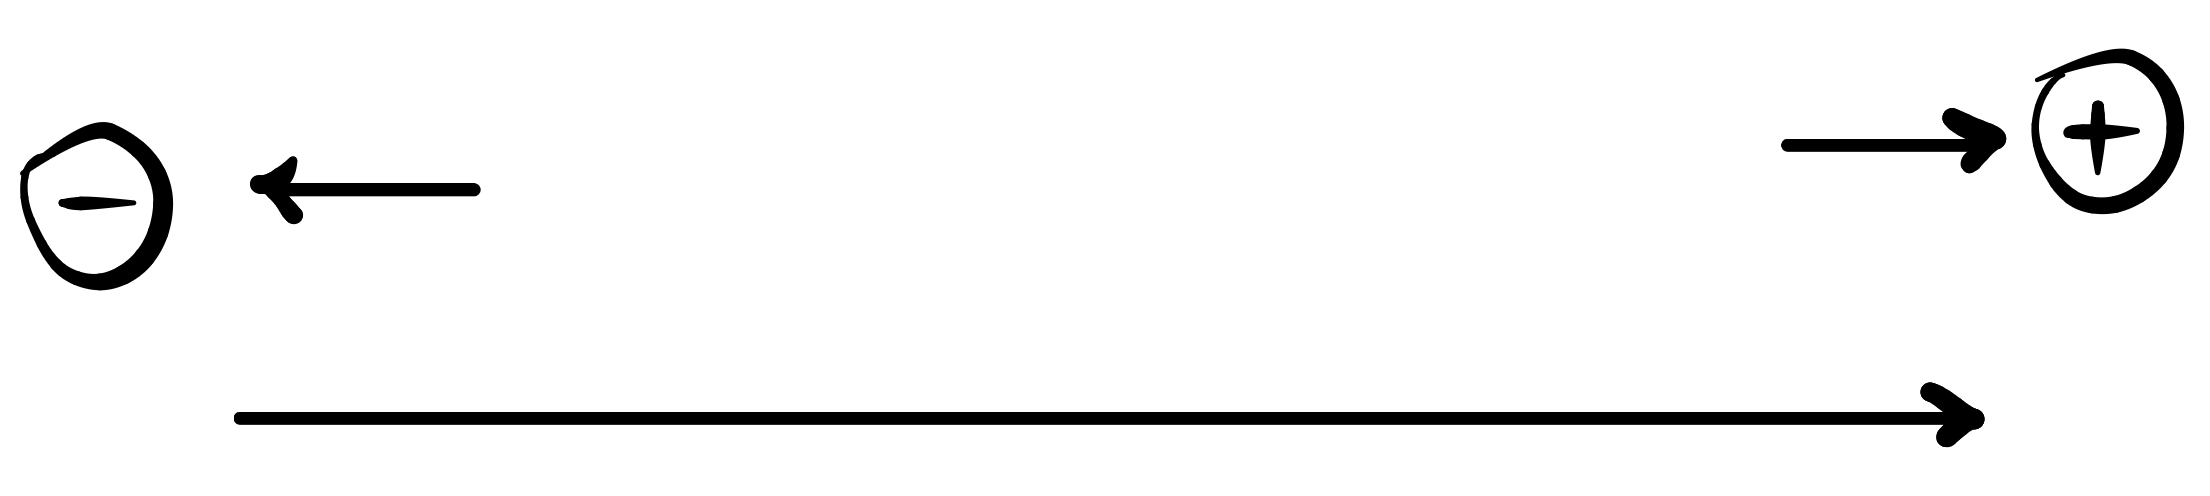
\includegraphics[scale=0.10]{imagenscinematicavetorial/grandezaescalar.jpeg}
    \caption{Em um movimento unidimensional a direção já está definida -- ela é única -- e o sentido pode ser expresso por dois sinais diferentes.}
    \label{fig_cinvet_grandezaescalar}
\end{figure}

Logo, se lhe for dito que um corpo possui velocidade de $-30$ km/h, você terá toda a informação necessária: você sabe a rapidez com que ele se move (valor absoluto da velocidade), você já sabe que ele se move na horizontal (direção do movimento) e, por conta do sinal, sabe que ele se move para a esquerda (sentido do movimento). Note que, para especificar com precisão para aonde um corpo se move, é fundamental saber essas três informações:

\begin{enumerate}
    \item [(i)] O valor absoluto da velocidade -- isso indica a rapidez com o corpo se move.
    \item [(ii)] A direção do movimento -- se ele ocorre na horizontal, na vertical, na diagonal, etc.
    \item [(iii)] O sentido do movimento: caso o movimento se dê na direção vertical, há duas possibilidades para o sentido: para cima ou para baixo. Se a direção for horizontal, o movimento pode ter sentido para direita ou para esquerda; etc.
\end{enumerate}


Perceba, contudo, que ao lhe informar que um corpo parte do ponto $P$ com velocidade de $30$ km/h, existem uma infinidade de movimentos possíveis, como mostra a primeira imagem da Figura \ref{fig_cinvet_grandezavetorial}: todas as direções são possíveis. Poderíamos especificar a direção, dizendo que é aquela que faz um ângulo de $60^\circ$ com a horizontal, como mostra a segunda imagem. Contudo, isso ainda seria insuficiente, posto que o corpo poderia se mover para um lado ou para o outro ao longo de tal direção -- ainda restariam duas opções possíveis.

\begin{figure}[h]
    \centering
    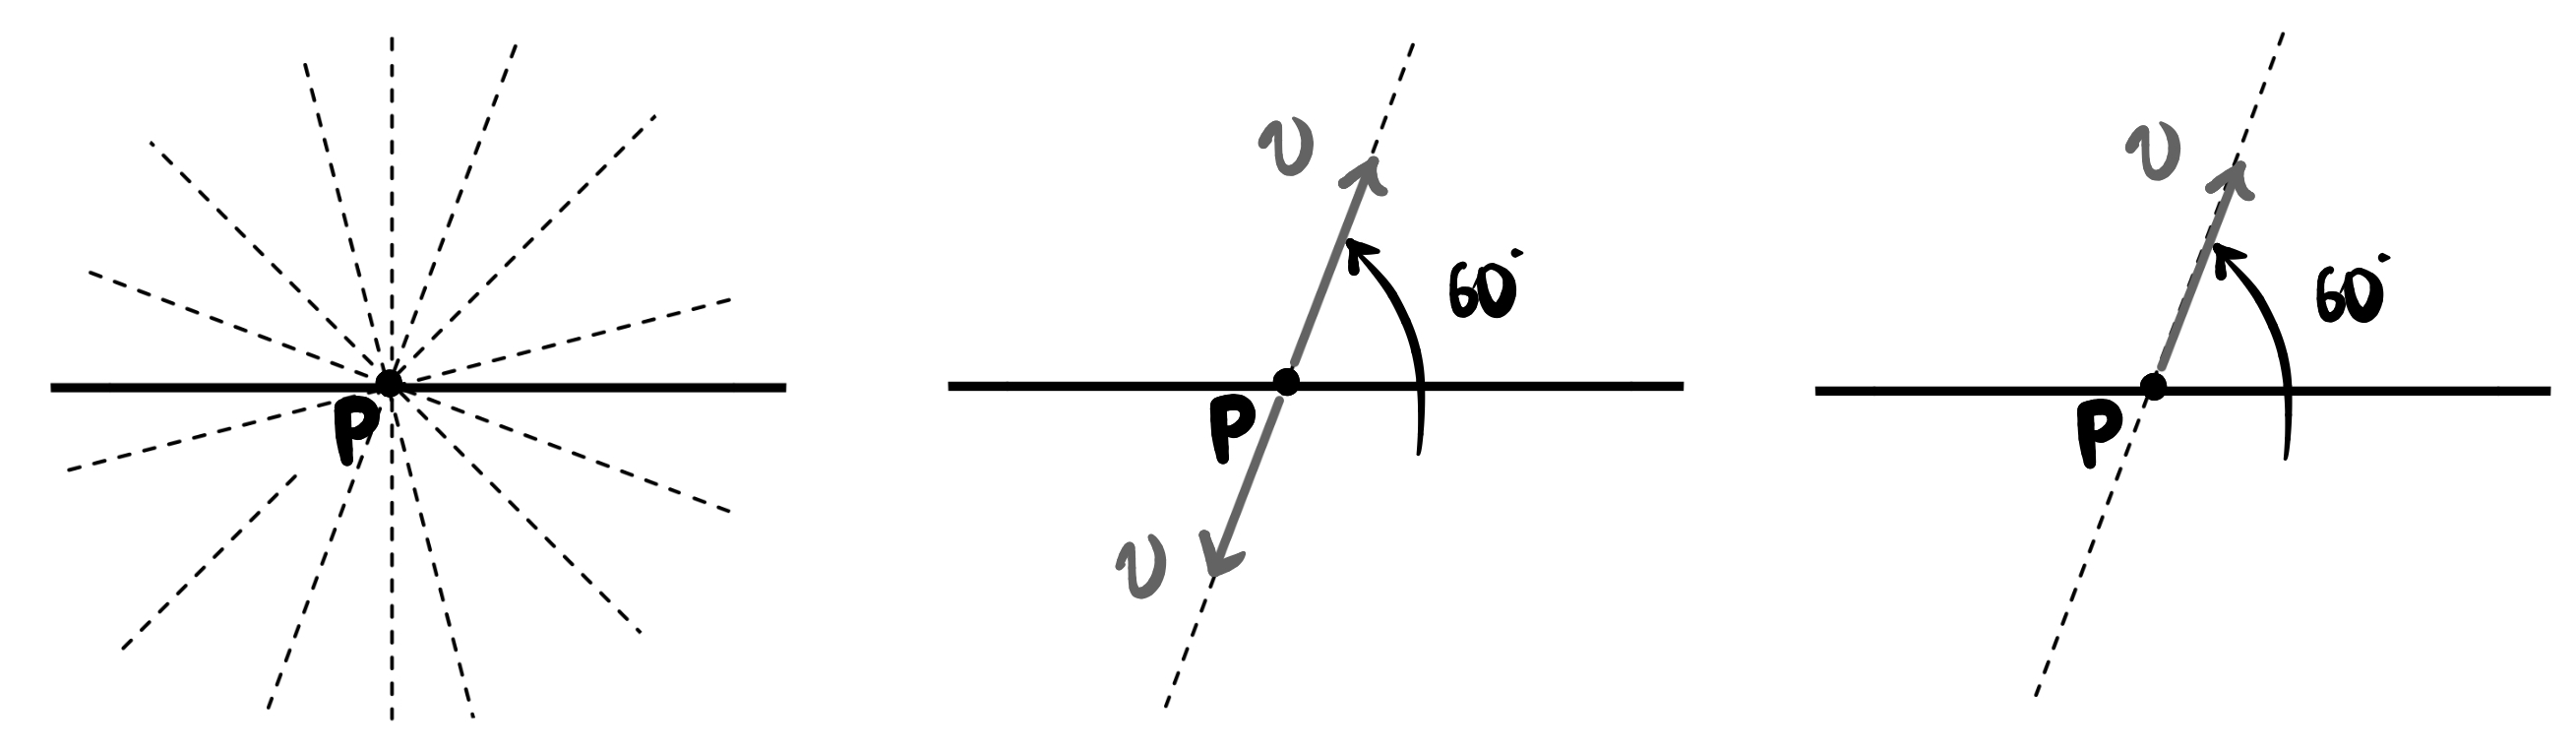
\includegraphics[scale=0.12]{imagenscinematicavetorial/grandezavetorial.jpeg}
    \caption{Para determinar com precisão o movimento é preciso informar o valor da velocidade, sua direção e seu sentido.}
    \label{fig_cinvet_grandezavetorial}
\end{figure}

Se afunilarmos e cravarmos que o corpo se move ``para cima'' -- ou seja, o sentido do movimento --, aí sim teremos transmitido toda a informação necessária para especificar o movimento -- a última imagem da Figura \ref{fig_cinvet_grandezavetorial} mostra isso.  \\



\begin{figure}[h]
    \centering
    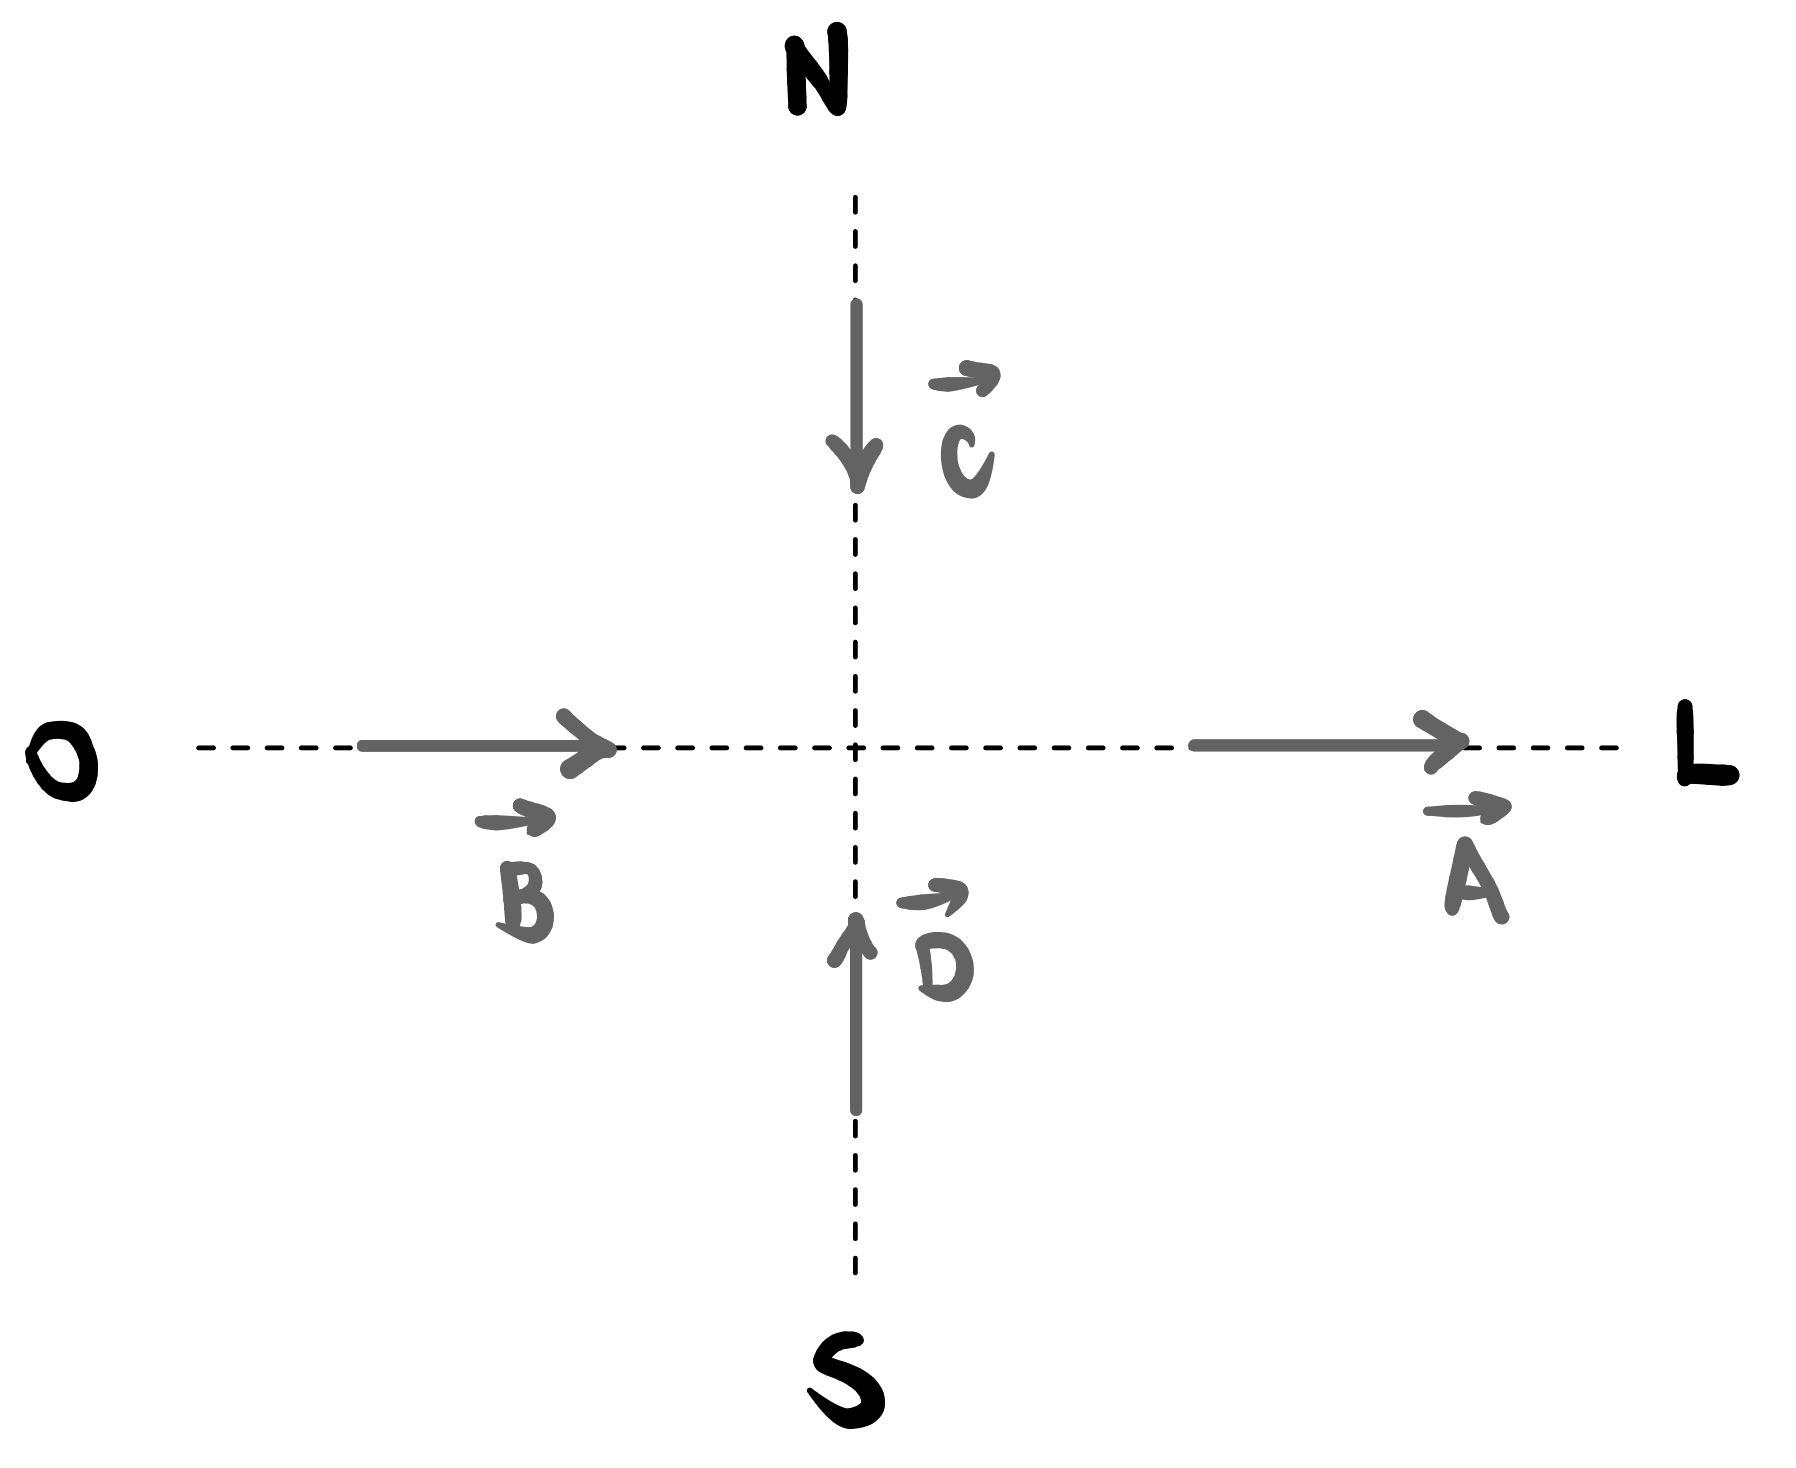
\includegraphics[scale=0.10]{imagenscinematicavetorial/vetordirecaosentido.jpeg}
    \caption{A diferença entre direção e sentido.}
    \label{fig_cinvet_vetordirecaosentido}
\end{figure}



Existem, portanto, certas grandezas que exigem que se informe não apenas seu valor, mas sua direção e sentido para que a informação transmitida esteja completa. Tais grandezas são chamadas de \textbf{grandezas vetoriais}, sendo a velocidade, a aceleração e a força alguns exemplos. Representaremos tais grandezas por setas, uma vez que uma seta consegue carregar essas três informações:

\begin{enumerate}
    \item [(i)] O valor da grandeza vetorial estará associado ao tamanho da seta. Logo, uma velocidade de $40$ km/h será representada por uma seta de tamanho $40$, enquanto uma velocidade de $20$ km/h será representada por uma seta com metade do tamanho. Chamamos isso de módulo do vetor e ele representa seu valor absoluto. Geometricamente, trata-se do tamanho da seta.
    \item [(ii)] A direção será determinada pela direção da seta\footnote{Que, normalmente, será especificada com base no ângulo que a seta faz com alguma direção -- normalmente, a horizontal.}. A Figura \ref{fig_cinvet_vetordirecaosentido} mostra, por exemplo, setas na direção vertical (norte-sul) e na direção horizontal (leste-oeste).
    \item [(iii)] Como uma seta pode apontar para dois sentidos diferentes em uma mesma direção, o sentido da seta irá indicar o sentido do vetor. No caso da Figura \ref{fig_cinvet_vetordirecaosentido} vemos que os vetores $\vec{A}$ e $\vec{B}$ possuem mesma direção (leste-oeste) e também o mesmo sentido: de oeste para leste (ou para a direita, caso prefira). Já os vetores $\vec{C}$ e $\vec{D}$ possuem a mesma direção (norte-sul, ou direção vertical), porém sentidos contrários.
\end{enumerate}







Representaremos uma grandeza vetorial, digamos, velocidade, por $\vec{v}.$ A seta em cima indica que se trata de um vetor. Perceba que a equação $\vec{v}=30$ km/h não faz sentido, porque estamos dizendo que uma seta -- um vetor -- é igual a um número, o que está claramente errado. Uma seta tem módulo, direção e sentido. O número, portanto, é só uma das características da seta -- está relacionada com o seu tamanho -- mas a seta é um ente geométrico que possui outras características além do tamanho.

Assim, para evitarmos esse tipo de incoerência, usaremos as seguinte notações quando quisermos nos referir ao tamanho do vetor, ou seja, seu módulo ou valor absoluto:

$$ v = |\vec{v}| = 30 \text{ km/h}.$$

Neste caso deixamos claro que estamos falando apenas de uma das características da seta: seu tamanho. A equação acima deve ser lida como \textit{o valor da velocidade é de 30 km/h} ou \textit{o módulo do vetor velocidade é de 30 km/h.} No caso da Equação \eqref{mecanica_eq_velocidaderelativa}, por exemplo, ela relaciona os \emph{módulos} das velocidades $v_A$ e $v_B$. Não introduzimos essa nomenclatura naquele contexto uma vez que a matemática dos vetores ainda não havia sido apresentada ao leitor.


Para lidar com movimentos que mudam de direção, movimentos curvilíneos e movimentos bidimensionais, de modo geral, o caráter vetorial de grandezas como velocidade ou aceleração será imprescindível. Desse modo, é importante que compreenda-se bem como funciona a matemática dos vetores.



\section{A Matemática dos Vetores}

Dentro do escopo do ensino médio existem essencialmente duas operações que podemos fazer com setas: multiplicar por uma constante (um escalar) ou somar/subtrair setas. Vamos entender em detalhes como funciona cada uma dessas operações.


\subsection{Multiplicação por Escalar}

Existem, além das grandezas vetoriais, as grandezas escalares. Enquanto os vetores precisam de módulo, direção e sentido para serem únicos, as grandezas escalares só precisam do módulo, isto é, do valor absoluto da grandeza. Um exemplo seria a temperatura. Se eu lhe disser que a temperatura ambiente está em $24^\circ$ Celsius você entendeu perfeitamente toda a informação necessária. A temperatura não aponta para lugar algum -- não precisa de direção ou sentido: é um escalar.

Grandezas escalares, portanto, são representadas apenas por um único número. Dito isso, nossa operação atual consiste em multiplicar um vetor por um escalar, ou seja, multiplicar um vetor por um número. O que essa operação faz é aumentar ou diminuir o tamanho de tal vetor, podendo, no máximo, inverter o seu sentido caso o número seja negativo.

A Figura \ref{fig_cinvet_multiplicarporescalar} mostra isso. Considere o vetor $\vec{A},$ que está na direção horizontal com sentido para a direita. Se multiplicarmos tal vetor por $2$ ou por $0,5$ teremos um vetor que terá, respectivamente, o dobro do tamanho e metade do tamanho do vetor $\vec{A};$ apontando, contudo, na mesma direção e sentido.

Poderíamos, contudo, multiplicar o vetor $\vec{A}$ por $-1$, o que nos daria um vetor de mesmo tamanho, mesma direção, porém sentido oposto. Já o vetor $-2\vec{A}$ possui a mesma direção, o dobro do tamanho e o sentido contrário ao de $\vec{A}.$


\begin{figure}[h]
    \centering
    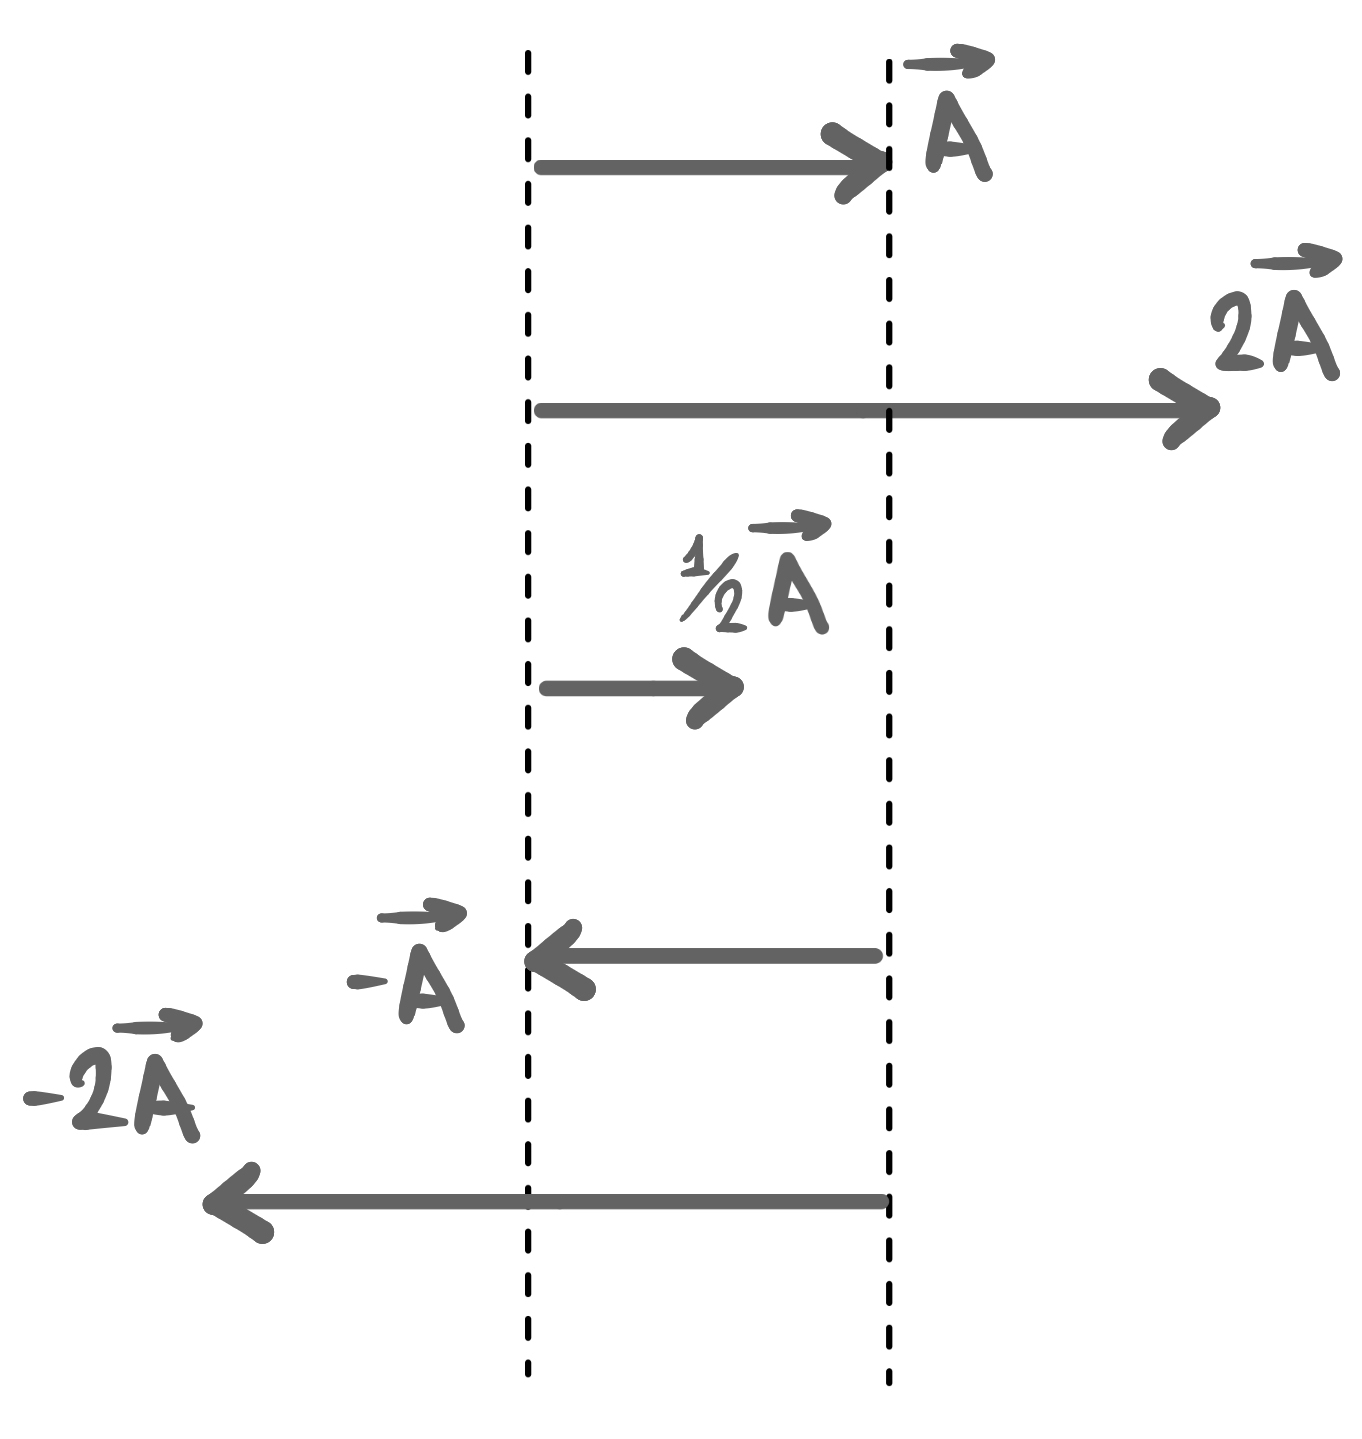
\includegraphics[scale=0.12]{imagenscinematicavetorial/dilatacaovetor.jpeg}
    \caption{A multiplicação de um vetor por um escalar.}
    \label{fig_cinvet_multiplicarporescalar}
\end{figure}


Note, portanto, que o efeito da multiplicação de um vetor por um escalar é o de dilatar ou contrair tal vetor: se o número for maior que $1$ (ou menor que $-1)$ nós estaremos aumentando o tamanho do vetor por tal fator multiplicativo. Já se o número for algo entre $0$ e $1$ (ou entre $-1$ e $0$) nós estaremos contraindo o vetor por tal fator multiplicativo. Além disso, tal operação permite que o sentido do vetor seja invertido -- caso o fator multiplicativo seja negativo -- mas nunca altera a direção original do vetor.



\subsection{Soma e Subtração}

Somar setas pode parecer uma operação estranha em um primeiro momento, mas veremos que ela é bem intuitiva. Imagine, como mostra a Figura \ref{fig_cinvet_somavetoresintro}, que você vai se deslocar do ponto $1$ até o ponto $2$ no espaço. Chegando no ponto $2,$ você se desloca até o ponto $3.$ Chegando lá, você vai para o ponto $4$ e, por fim, se desloca do ponto $4$ ao $5.$


\begin{figure}[h]
    \centering
    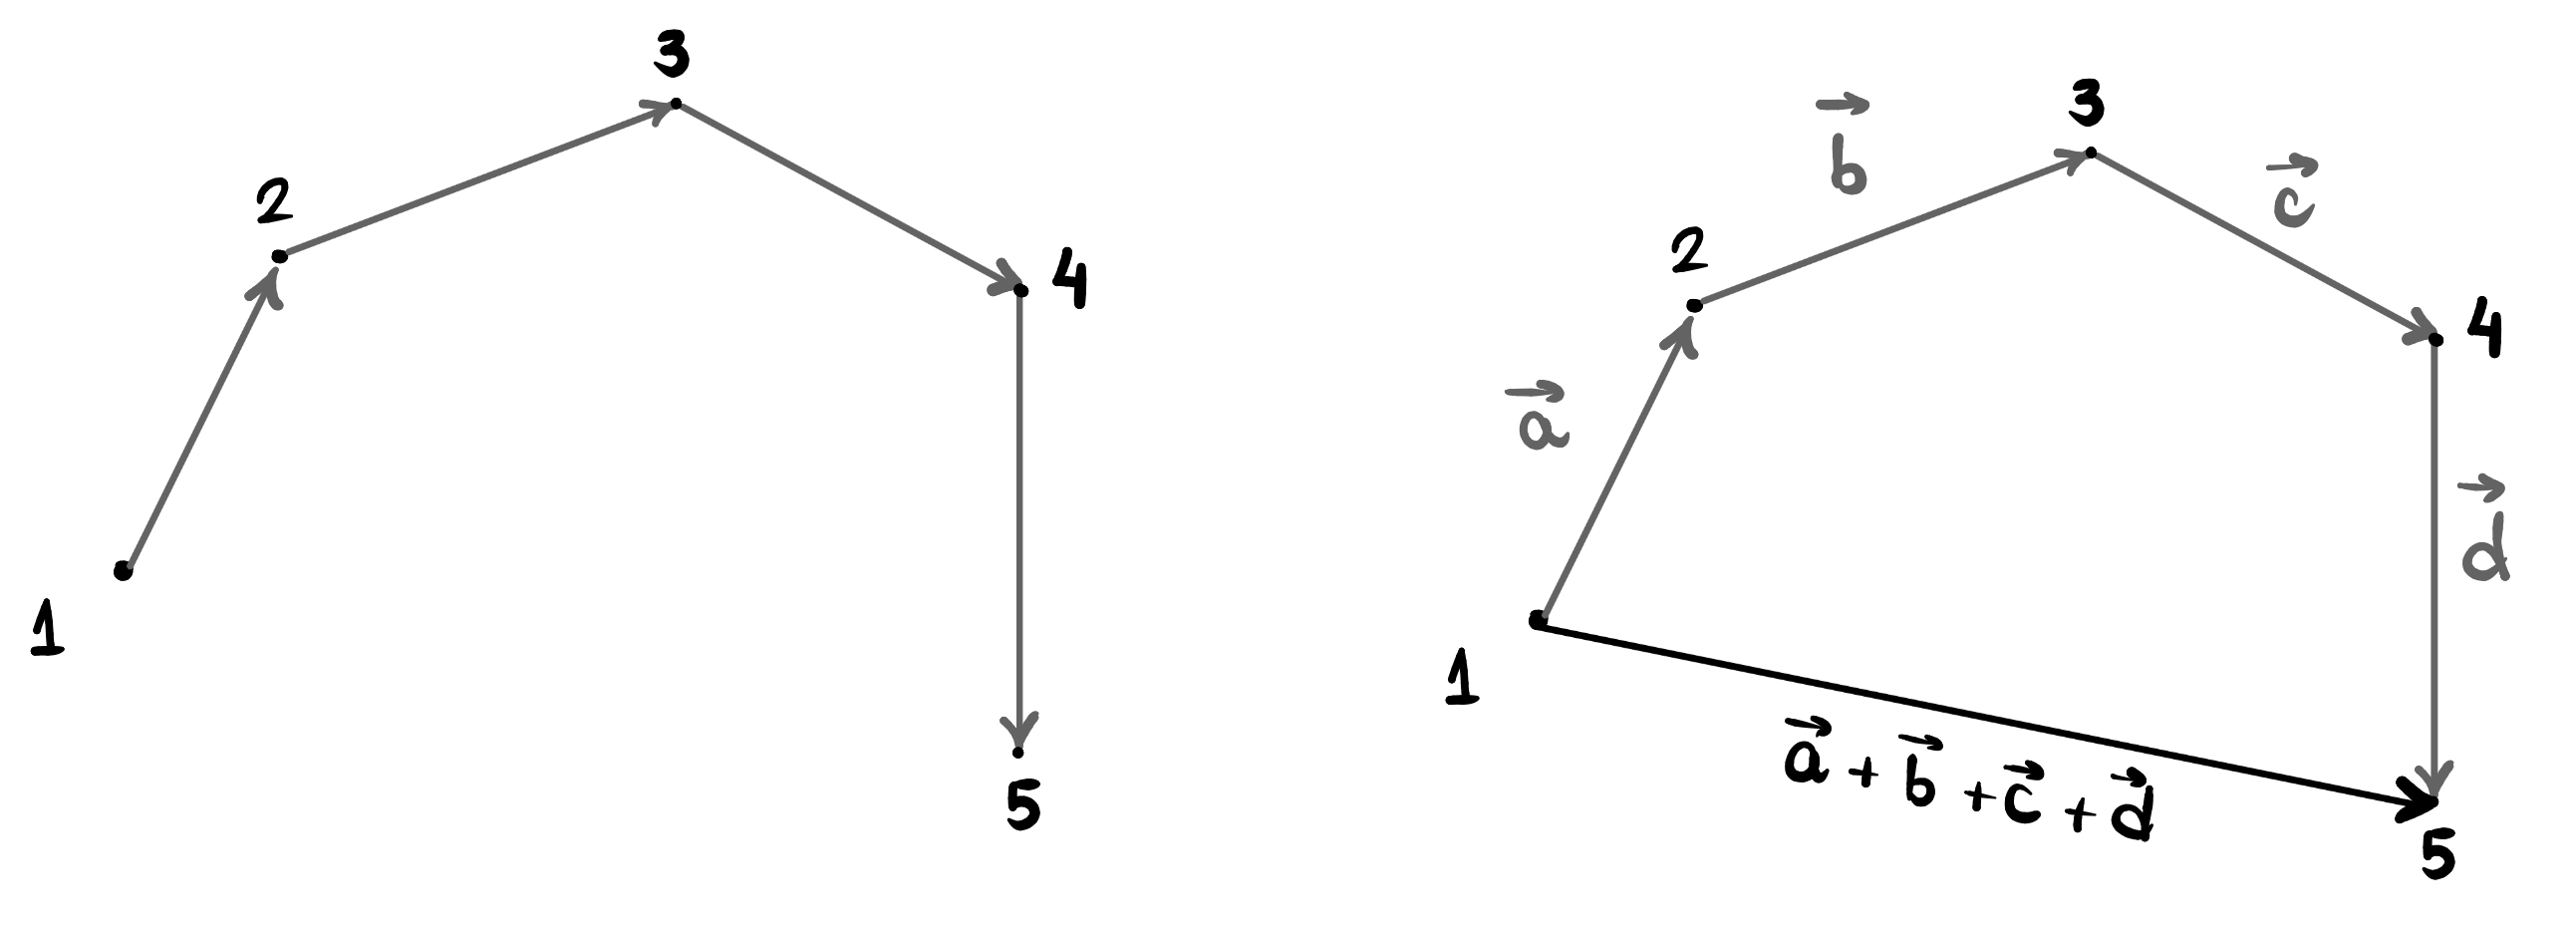
\includegraphics[scale=0.12]{imagenscinematicavetorial/somarsetasintro.jpeg}
    \caption{A soma dos vetores $\vec{a},\vec{b}, \vec{c} $ e $\vec{d}.$}
    \label{fig_cinvet_somavetoresintro}
\end{figure}

Temos aqui quatro setas que representam cada deslocamento que você teve ao longo do movimento. Como podemos somá-las? Ora, o efeito total do seu movimento foi sair do ponto $1$ e chegar ao ponto $5,$ desse modo, seu deslocamento total -- o quanto você se distanciou do ponto de partida -- é representado pela seta que une o ponto de partida (ponto $1)$ ao ponto de chegada (ponto $5$). Pronto: você acabou de aprender a lógica que guia a soma de setas.

De forma mais matemática, se os vetores em questão forem designados por $\vec{a},\vec{b}, \vec{c} $ e $\vec{d},$ o vetor soma $(\vec{a}+\vec{b}+\vec{c} +\vec{d})$\footnote{É importante que o leitor perceba a diferença entre a operação $(\vec{a}+\vec{b}+\vec{c} +\vec{d})$ e a operação $a+b+c+d$: a primeira envolve a soma de setas, enquanto a segunda envolve a soma de números -- que representam o tamanho das setas. Mais adiante vamos destacar com ainda mais ênfase essa diferença.} é aquele representado na segunda imagem da Figura \ref{fig_cinvet_somavetoresintro}.

A regra, portanto, é: para somar duas setas, conecte o início de uma delas com a extremidade da outra. A seta resultante é aquela que vai do início da primeira à extremidade da última. Isso vale para duas, três, cinco ou quarenta setas (vetores) que quisermos somar. Algumas perguntas poderiam surgir neste momento:

\begin{enumerate}
    \item [(i)] \textit{Mas e se os vetores em questão não forem referentes a um deslocamento?}

    Não mudaria nada. A lógica para se somar setas é sempre a mesma. Usamos os vetores $\vec{a},\vec{b}, \vec{c} $ e $\vec{d}$ como se fossem deslocamentos para deixar mais intuitivo a razão de essa ser a regra para se somar setas. Contudo, se os vetores $\vec{a},\vec{b}, \vec{c} $ e $\vec{d}$ representassem velocidades, acelerações ou forças, a operação de somá-los se daria exatamente do mesmo modo.
    
    \item [(ii)] \textit{Como poderíamos saber o tamanho do vetor resultante no caso da Figura \ref{fig_cinvet_somavetoresintro} ?}

    Essa seria uma ótima pergunta. O que se quer saber é, sabendo quais são os tamanhos das setas $\vec{a},\vec{b}, \vec{c} $ e $\vec{d}$, como podemos obter o tamanho da seta final? Essa será a pauta da nossa próxima discussão.
\end{enumerate}


Vamos à nobre tarefa de somar duas setas, digamos, $\vec{A}$ e $\vec{B},$ cujos tamanhos são 4 e 3, respectivamente. Ou seja, em notação matemática:

 $$|\vec{A}|=4 \quad \text{ e } \quad |\vec{B}|=3. $$

O leitor menos atento já poderia concluir que o vetor soma $(\vec{A}+\vec{B})$ será uma seta de tamanho $(4+3)=7,$ o que seria precipitado e, provavelmente, incorreto. Perceba que o tamanho da seta resultante irá depender das direções de cada uma das setas que serão somadas e, para cada uma delas, a geometria da soma será diferente. 

A nossa regra para somar os vetores será desenhá-los de modo que o início de um deles coincida com a extremidade do outro e, a partir disso, o vetor resultante será aquele que vai do início do primeiro à extremidade do último. Veja o resultado que tal regra nos daria no caso da Figura \ref{fig_cinvet_somasetas01}\footnote{Uma seta não possui lugar fixo no espaço, de modo que o leitor tem liberdade de desenhá-la aonde ele quiser: desde que possua o mesmo módulo, mesma direção e mesmo sentido, tratar-se-á sempre do mesmo vetor, independente da posição em que ele está desenhado.}.

Na primeira imagem temos os vetores $\vec{A}$ e $\vec{B},$ na imagem do meio temos eles desenhados de modo que o início de um deles coincida com a extremidade do outro, e na terceira imagem temos a regra da soma aplicada: o vetor soma é o que vai da origem do primeiro à extremidade do último. Note que, neste caso, sendo os tamanhos dos vetores $\vec{A}$ e $\vec{B}$ iguais a $4$ e $3,$ o nosso vetor soma terá, de fato, um tamanho que é igual à soma dos tamanhos dos vetores somados: $4+3=7.$


\begin{figure}[h]
    \centering
    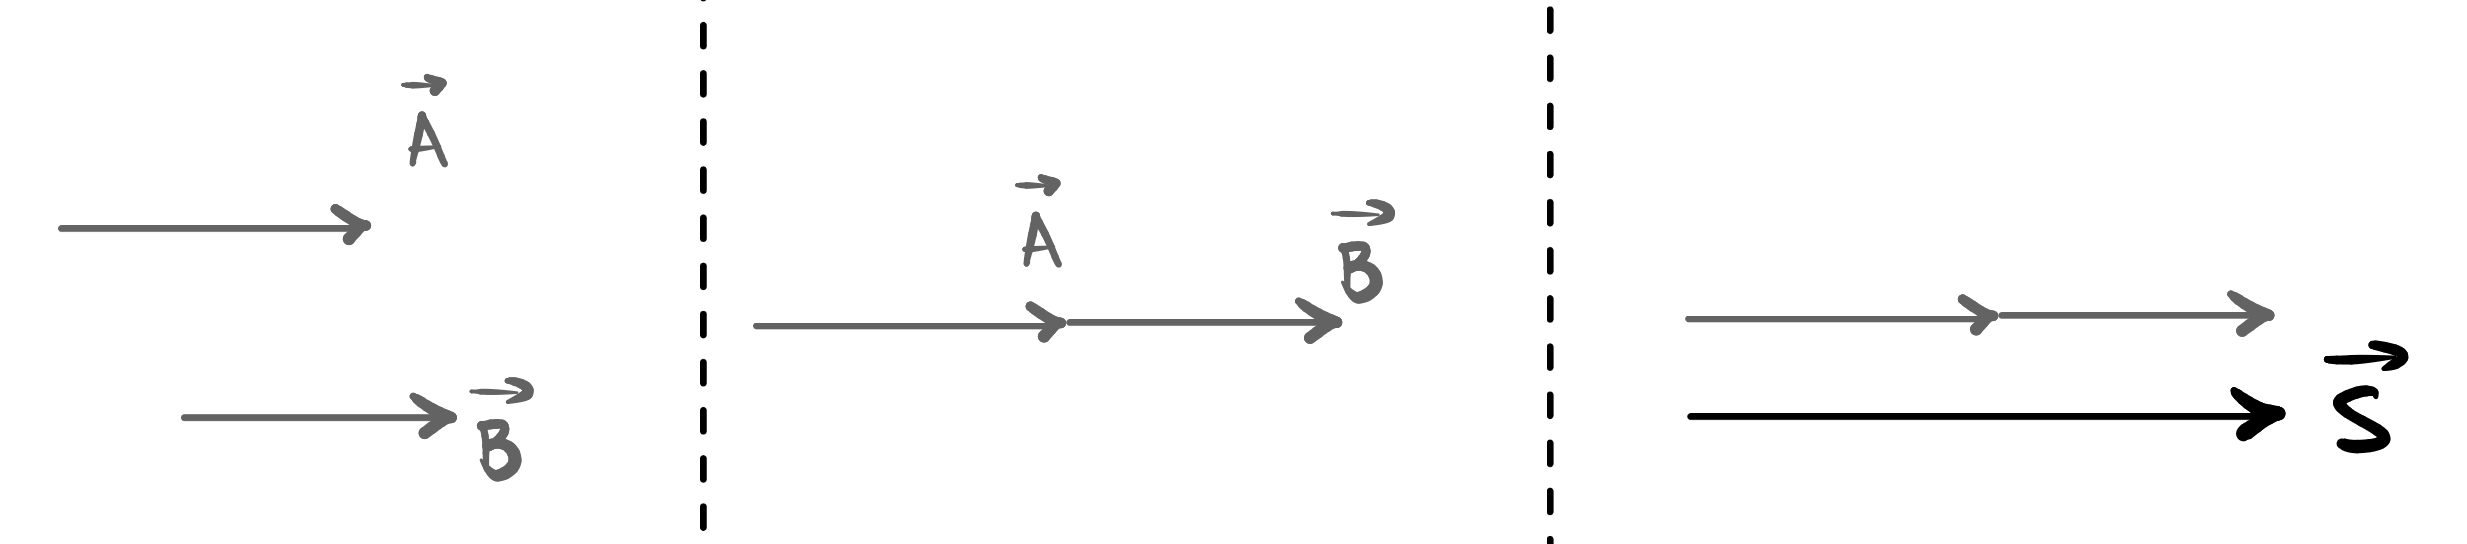
\includegraphics[scale=0.12]{imagenscinematicavetorial/somarvetores1.jpeg}
    \caption{Somando os vetores $\vec{A}$ e $\vec{B}$ de mesma direção e sentido.}
    \label{fig_cinvet_somasetas01}
\end{figure}

Perceba, contudo, os mesmos vetores $\vec{A}$ e $\vec{B}$ de tamanhos $4$ e $3,$ porém de sentidos opostos, como no contexto da Figura \ref{fig_cinvet_somasetas02}.


\begin{figure}[h]
    \centering
    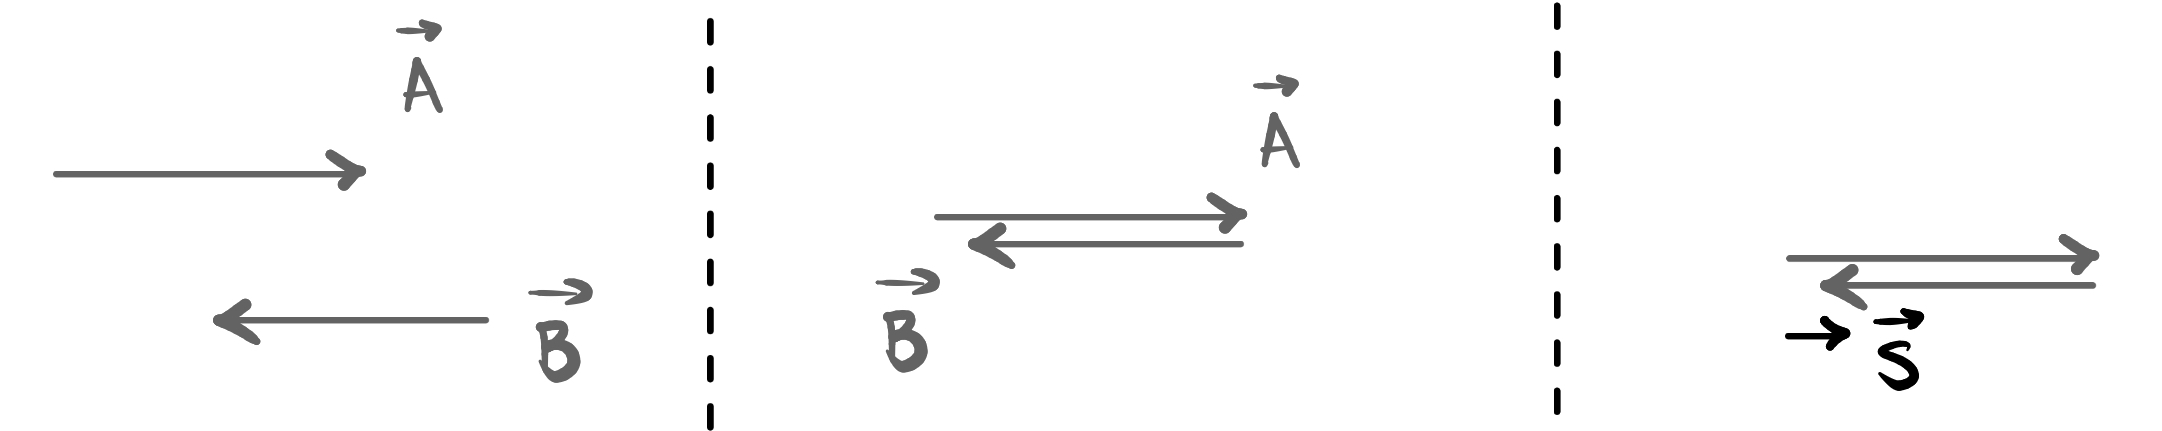
\includegraphics[scale=0.135]{imagenscinematicavetorial/somarvetores2.jpeg}
    \caption{Somando os vetores $\vec{A}$ e $\vec{B}$ de mesma direção e sentidos opostos.}
    \label{fig_cinvet_somasetas02}
\end{figure}


Neste caso, o vetor que vai da origem de $\vec{A}$ até a extremidade de $\vec{B}$ terá um tamanho dado por $4-3=1,$ como mostra a geometria da situação na Figura \ref{fig_cinvet_somasetas02}.

Já se alterarmos as direções dos vetores $\vec{A}$ e $\vec{B}$ para a situação da Figura \ref{fig_cinvet_somasetas03}, em que tais vetores tenham direções perpendiculares, notaremos agora que o tamanho da seta resultante será dado pelo Teorema de Pitágoras, ou seja, será igual a

$$ \sqrt{3^2+4^2}=5.$$

\begin{figure}[h]
    \centering
    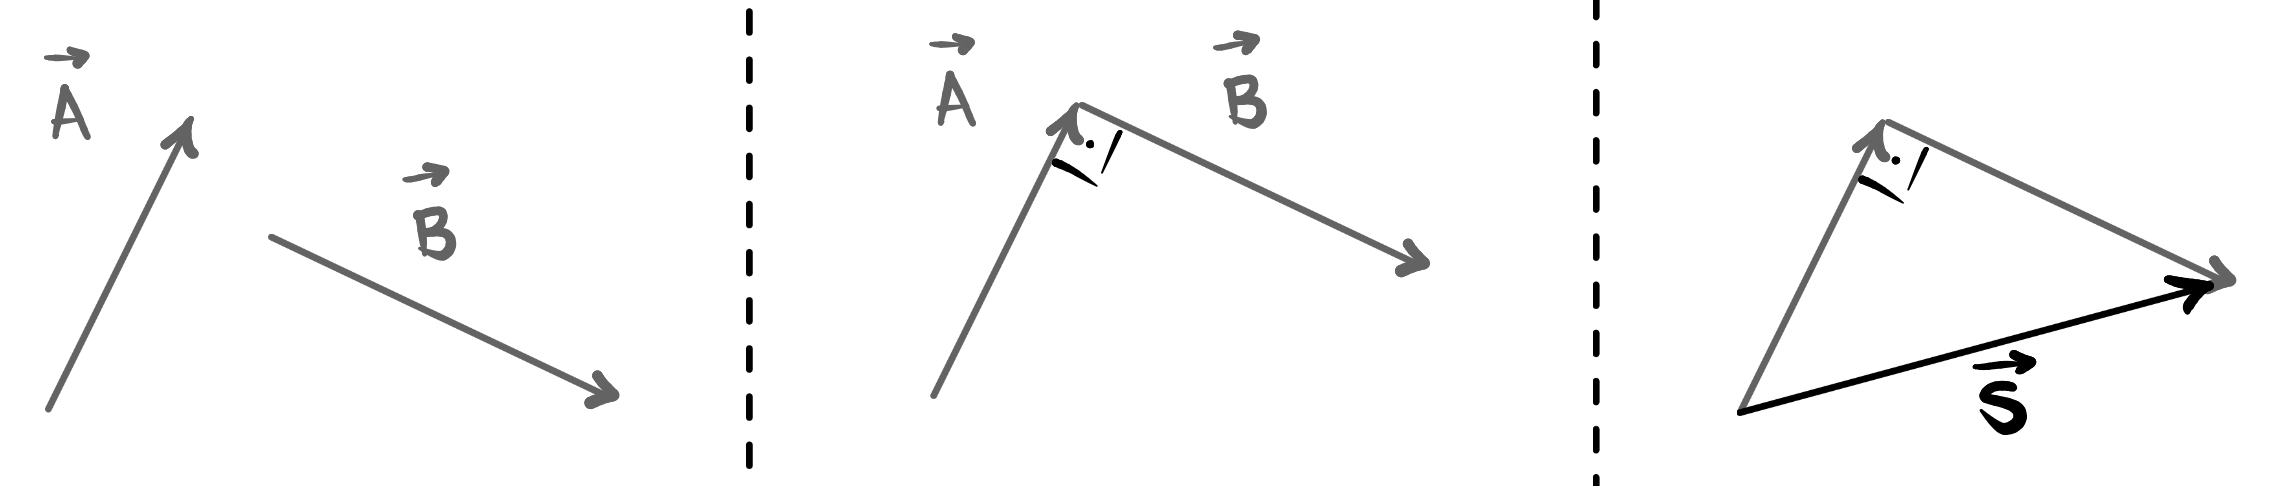
\includegraphics[scale=0.12]{imagenscinematicavetorial/somarvetores3.jpeg}
    \caption{Somando os vetores $\vec{A}$ e $\vec{B}$ de direções perpendiculares.}
    \label{fig_cinvet_somasetas03}
\end{figure}

Por fim, se as direções dos vetores $\vec{A}$ e $\vec{B}$ fizerem um ângulo de $120$ graus, como mostra a Figura \ref{fig_cinvet_somasetas04}, ao aplicar a mesma regra de soma, seremos levados a uma geometria que nos obrigaria a aplicar a Lei dos Cossenos, que forneceria como resultado que o tamanho da seta resultante da soma das setas $\vec{A}$ e $\vec{B}$ seria

$$ \sqrt{3^2+4^2- 2 \cdot 4\cdot 3 \cdot \cos(120^\circ)} = \sqrt{37} \approx 6{,}08. $$

\begin{figure}[h]
    \centering
    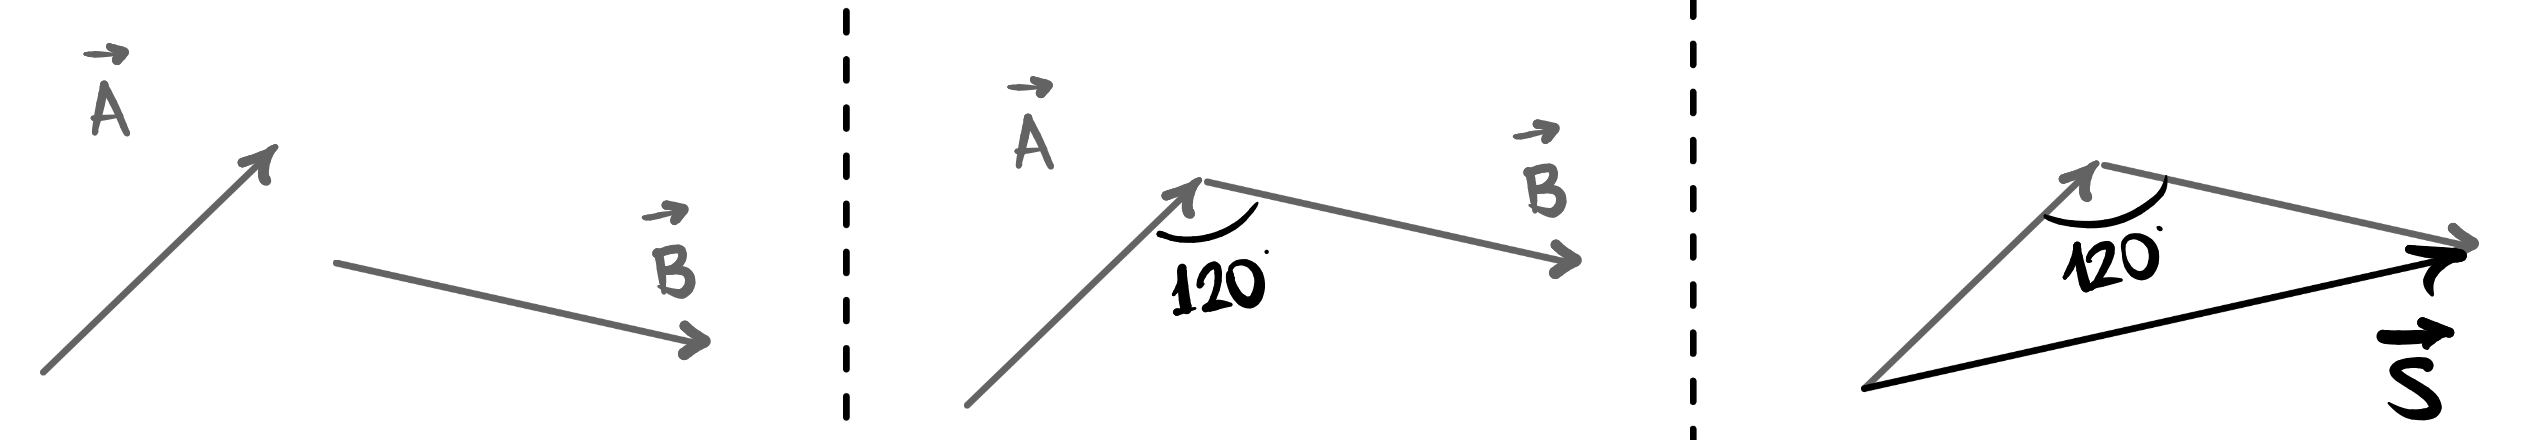
\includegraphics[scale=0.12]{imagenscinematicavetorial/somarvetores4.jpeg}
    \caption{Somando os vetores $\vec{A}$ e $\vec{B}$ de direções que fazem um ângulo obtuso.}
    \label{fig_cinvet_somasetas04}
\end{figure}



Sendo assim, o problema de obter o tamanho da seta resultante a partir da soma de outras duas setas é um problema de geometria. Para cada direção e sentido das setas somadas a geometria será uma, de modo que, para setas, $3+4$ nem sempre dá $7.$ 

Como vimos, é possível somar setas de tamanhos $3$ e $4$ e obter como resultado uma seta cujo tamanho dá $1$, ou $5$, ou $6{,}08$ ou até mesmo o próprio $7.$ Ao somar vetores de módulos $3$ e $4$ poderemos obter, para o tamanho do vetor resultante, qualquer valor entre $1$ e $7$ -- os casos das Figuras \ref{fig_cinvet_somasetas01} e \ref{fig_cinvet_somasetas02} são os extremos. Quando as setas possuem a mesma direção e mesmo sentido teremos um valor máximo para o tamanho da seta resultante; já quando elas possuem mesma direção e sentidos opostos teremos um valor mínimo para o tamanho da seta resultante. Qualquer outra configuração geométrica diferente dessas fornecerá um valor de tamanho para a seta resultante entre $1$ e $7.$


Logo, olhando para a situação da Figura \ref{fig_cinvet_somavetoresintro}, é impossível sabermos o tamanho da seta resultante sem sabermos exatamente o tamanho e os ângulos que as setas $\vec{a},\vec{b}, \vec{c} $ e $\vec{d}$ fazem entrem si, uma vez que são eles que definem a geometria do problema.


Por fim, vamos comentar sobre a operação de subtrair setas. Digamos que queremos fazer a subtração do vetor $\vec{B}$ do vetor $\vec{A},$ isto é, computar $(\vec{A}-\vec{B})$. Ora, note que isso é o mesmo que somar o vetor $\vec{A}$ com o vetor $-\vec{B},$ ou seja:

$$ \vec{A}-\vec{B} = \vec{A} + (- \vec{B}),$$

\noindent ou seja, uma vez que sabemos que $-\vec{B}$ é simplesmente o vetor $\vec{B}$ apontando no sentido oposto, acabamos de converter a subtração em uma soma: fazer a subtração $(\vec{A}-\vec{B})$ é somar o vetor $\vec{A}$ com o oposto do vetor $\vec{B},$ isto é, com $-\vec{B}$. A Figura \ref{fig_cinvet_subtrairsetas} mostra, na primeira coluna, a operação da soma dos vetores $\vec{A}$ e $\vec{B}$, enquanto a segunda coluna mostra a diferença entre os vetores.

\begin{figure}[h]
    \centering
    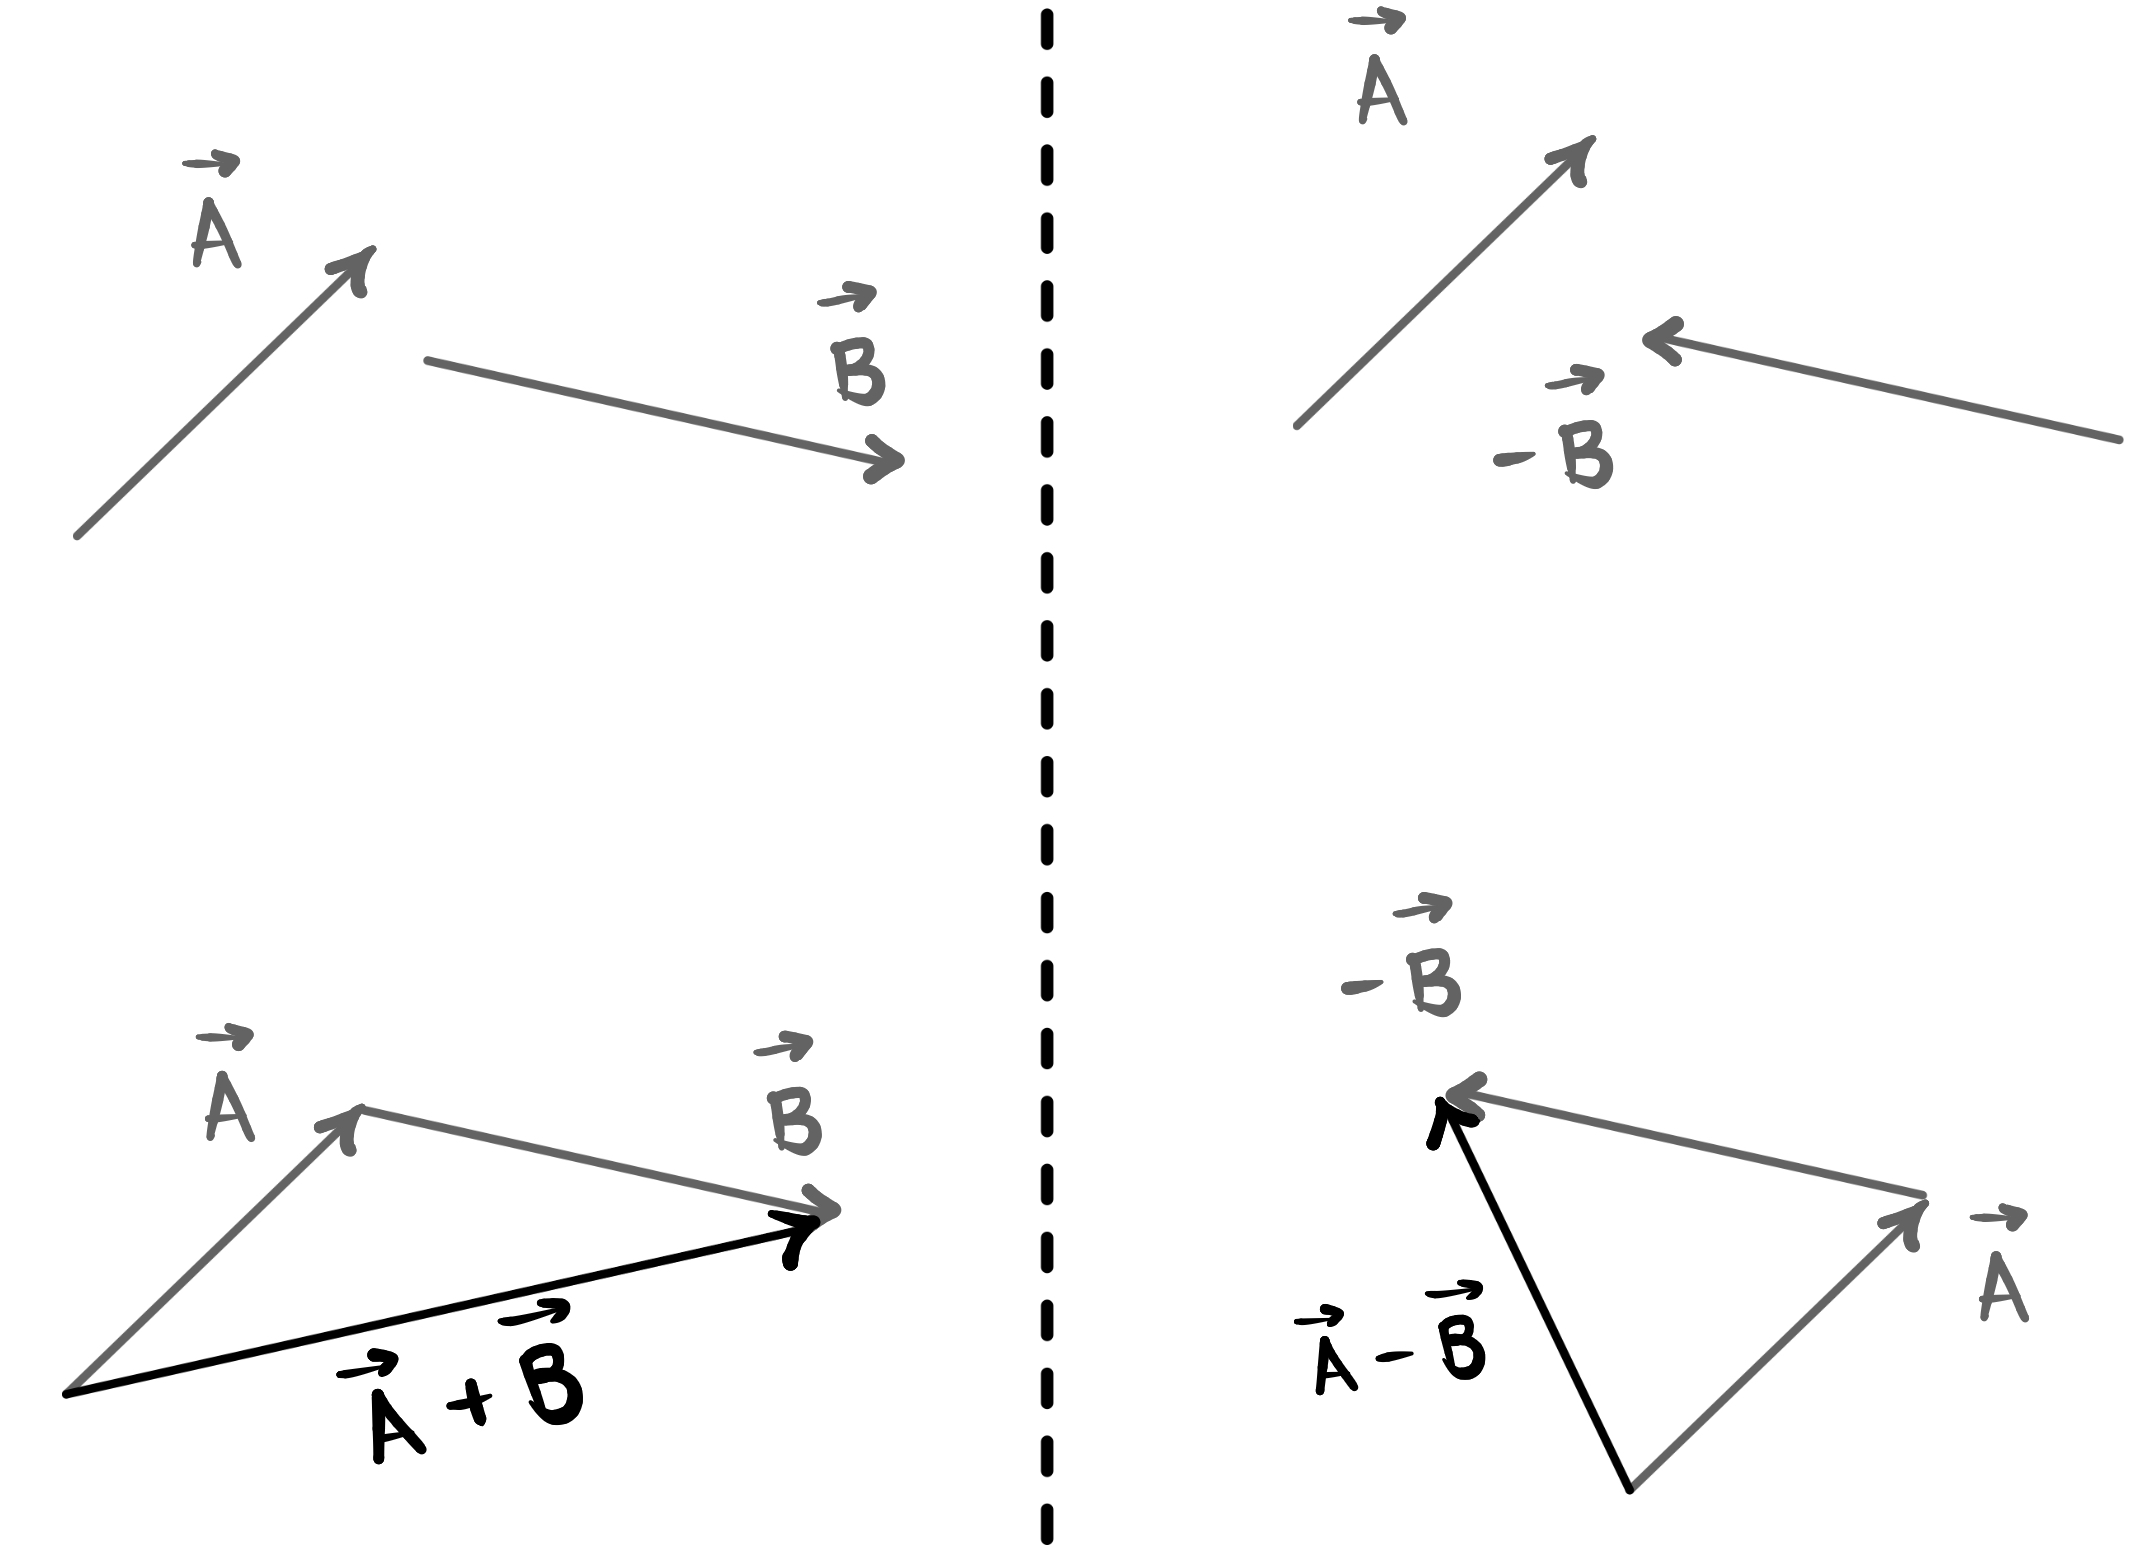
\includegraphics[scale=0.12]{imagenscinematicavetorial/subtrairvetores.jpeg}
    \caption{A soma e a subtração dos vetores $\vec{A}$ e $\vec{B}.$}
    \label{fig_cinvet_subtrairsetas}
\end{figure}


Curiosamente uma operação muito comum de se fazer com setas é o inverso do que construímos anteriormente. Ou seja, ao invés de lhe dar dois vetores e perguntar qual é o vetor resultante; teremos um único vetor e vamos querer entender quais são os outros dois vetores que, somados, dão ele.

É como se, em uma direção, estivéssemos fazendo a soma de $3+4,$ que naturalmente dá $7$ (estamos pensando em apenas números agora). Porém, neste momento, seremos apresentados ao número $7$, e buscaremos entender quais são os números que somados resultam nele. Perceba que essa pergunta pode ter várias respostas, dependendo do campo numérico que estivermos considerando. Ou seja, dado o número $7$, os dois números somados que resultam nele podem ser:

\begin{enumerate}
    \item [(i)] $3$ e $4$ caso estejamos restritos ao campo dos números naturais.
    \item [(ii)] $-5$ e $12$ caso ampliemos nosso escopo para os números inteiros (que incluem os negativos). Neste caso já teríamos várias outras possibilidades, como $-1$ e $8$ ou $-2$ e $9,$ por exemplo.
    \item [(iii)] $5.5$ e $1.5$ caso ampliemos nosso escopo para os números racionais (que incluem as frações). Neste também teríamos várias outras possibilidades, como $3.5$ e $3.5$ ou $-1.5$ e $8.5$, por exemplo.
\end{enumerate}

Perceba, portanto, que quando se somam dois números (ou duas setas) a resposta é única; porém, ao lhe ser entregue um número (ou uma seta), existirão várias possibilidades de pares de números (ou de setas) que, somados, dão como resultado o primeiro número.

No caso dos vetores, a ambiguidade tem a ver com a direção a ser escolhida para os vetores que, somados, darão o primeiro. Considere a Figura \ref{fig_cinvet_decomporvetores1}, que mostra, na primeira imagem, um dado vetor $\vec{A}.$ Queremos achar os dois vetores que, somados, resultam no vetor $\vec{A.}$ Na segunda imagem da figura foi fixada duas direções perpendiculares $x$ e $y$ -- as direções horizontal e vertical, respectivamente. Neste caso, fixadas essas direções, nossa resposta será única -- é como se estivéssemos nos restringindo ao campo dos números naturais, pensando em soma de números. Ou seja, a pergunta agora não é \textit{quais são os dois vetores que, somados, resultam no vetor A?}, mas sim \textit{quais são os dois vetores -- estando cada um deles nas direções $x$ e $y$ escolhidas -- que, somados, resultam no vetor A?}.


\begin{figure}[h]
    \centering
    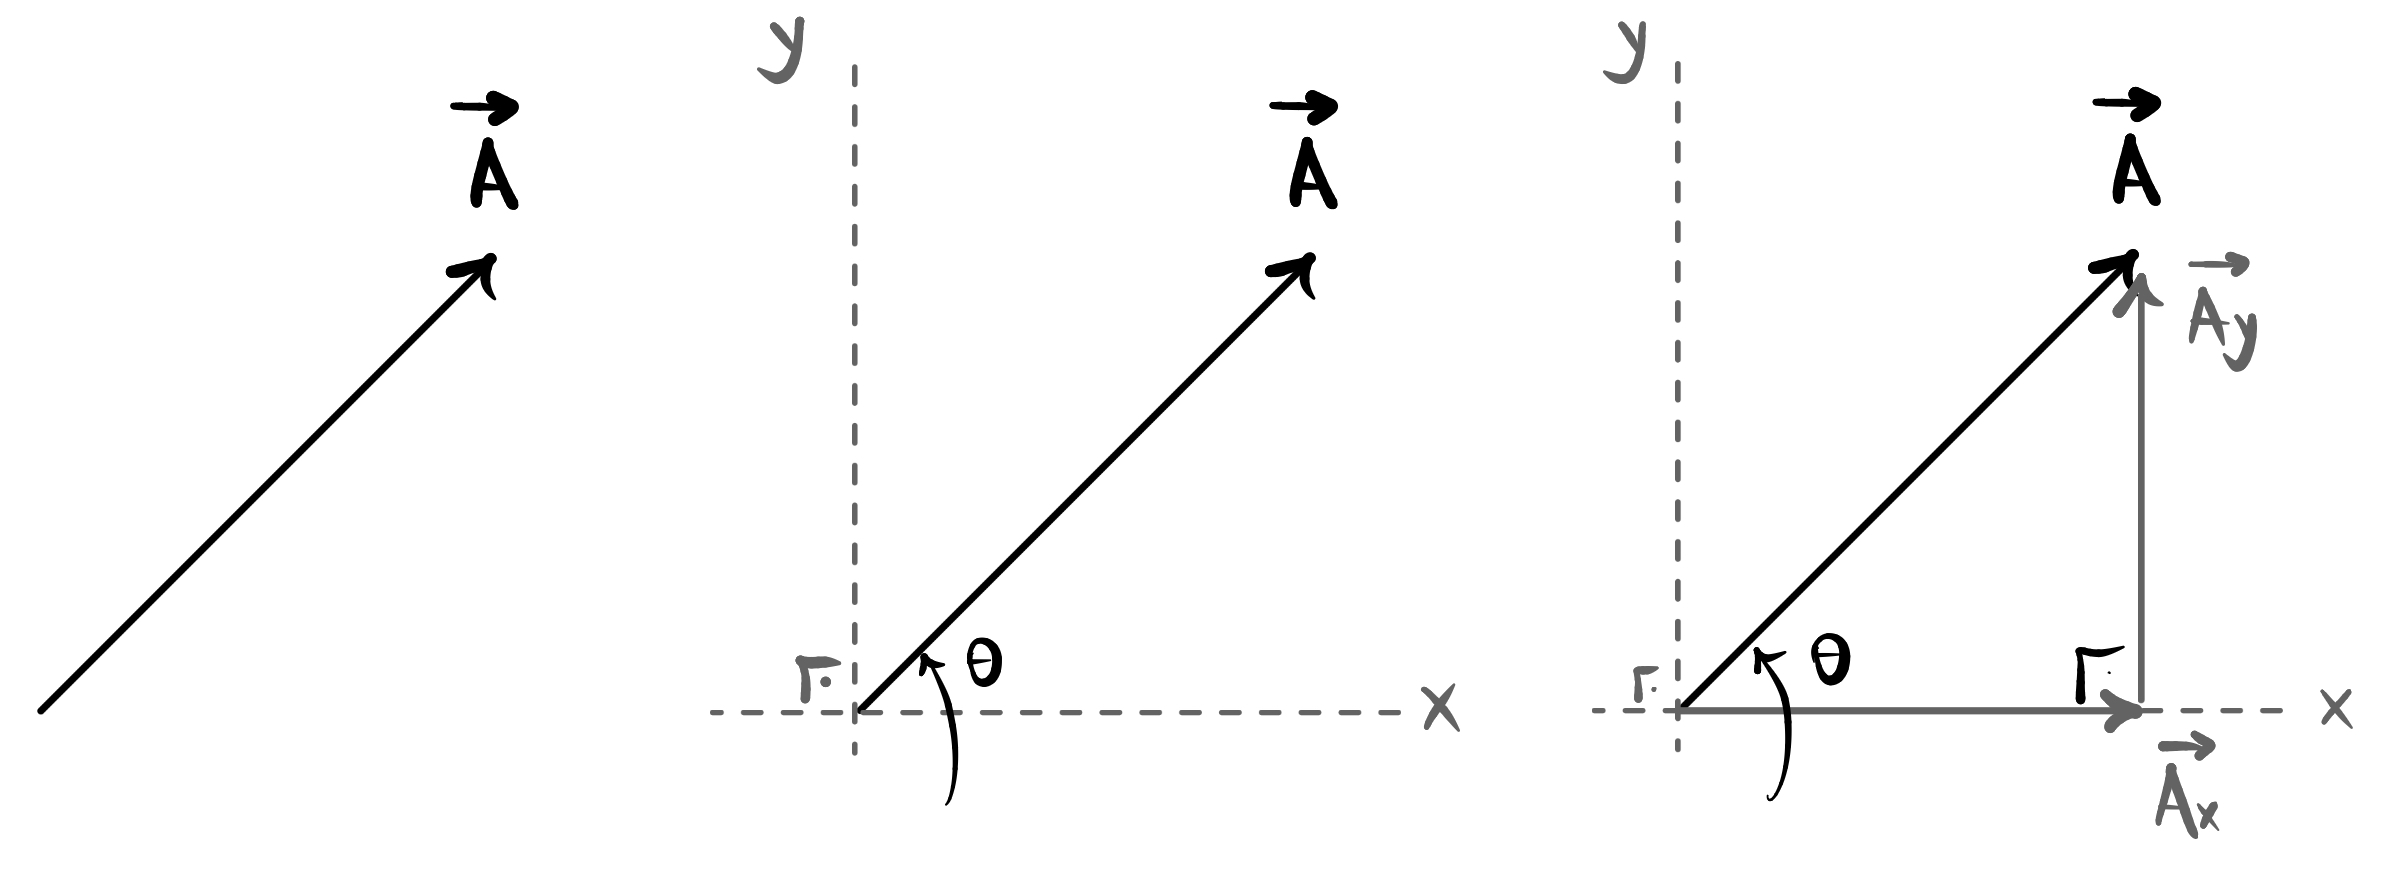
\includegraphics[scale=0.15]{imagenscinematicavetorial/decomporvetores1.jpeg}
    \caption{A decomposição vetorial nas direções cartesianas horizontal e vertical.}
    \label{fig_cinvet_decomporvetores1}
\end{figure}


Perceba, na última imagem, que os vetores $\vec{A}_x$ e $\vec{A}_y$, se somados, resultam no vetor $\vec{A},$ isto é:

$$ \vec{A} = \vec{A}_x + \vec{A}_y, $$

\noindent como queríamos. Ou seja, dado um vetor $\vec{A}$ encontramos os dois vetores $\vec{A}_x$ e $\vec{A}_y$ que, somados, resultam nele. Sendo as direções $x$ e $y$ perpendiculares, os módulos de tais vetores podem ser relacionados pelo Teorema de Pitágoras, isto é

$$ A^2 = A_x^2 + A_y^2,$$

\noindent e essa é a principal razão de se escolher direções perpendiculares -- para que valha o Teorema de Pitágoras na relação entre os módulos dos vetores. Poderíamos também relacionar o módulo de cada novo vetor $A_x$ e $A_y$ com o módulo $A$ do vetor inicial e o ângulo $\theta$ que ele faz com uma das direções escolhidas. Isso é feito usando a definição das razões trigonométricas no triângulo retângulo da terceira imagem da figura, de onde tiramos que

$$ \sin \theta = \dfrac{A_y}{A} \implies \boxed{A_y = A \sin \theta} \quad  \text{ e } \quad \cos \theta = \dfrac{A_x}{A} \implies \boxed{A_x = A \cos \theta.} $$

Esse é mais um motivo para usarmos direções perpendiculares na decomposição dos vetores: as relações trigonométricas acima são definidas e, portanto, só valem em triângulos retângulos.

O que acabamos de fazer foi uma \textbf{decomposição vetorial}: dado um vetor $\vec{A}$ e duas direções $x$ e $y$ encontramos quem são os vetores $A_x$ e $A_y$ ao longo de tais direções que, somados, resultam no vetor inicial $\vec{A}.$ Por isso, os vetores $\vec{A}_x$ e $\vec{A}_y$ são chamados de componentes do vetor $\vec{A.}$

Perceba que, se soubermos o módulo $A$ do vetor inicial $\vec{A}$ e qual é o ângulo $\theta$ que ele faz com alguma das direções escolhidas, as equações acima nos permitem calcular o módulo das suas componentes $A_x$ e $A_y$ e, portanto, resolver o problema proposto inicialmente.

\begin{figure}[h]
    \centering
    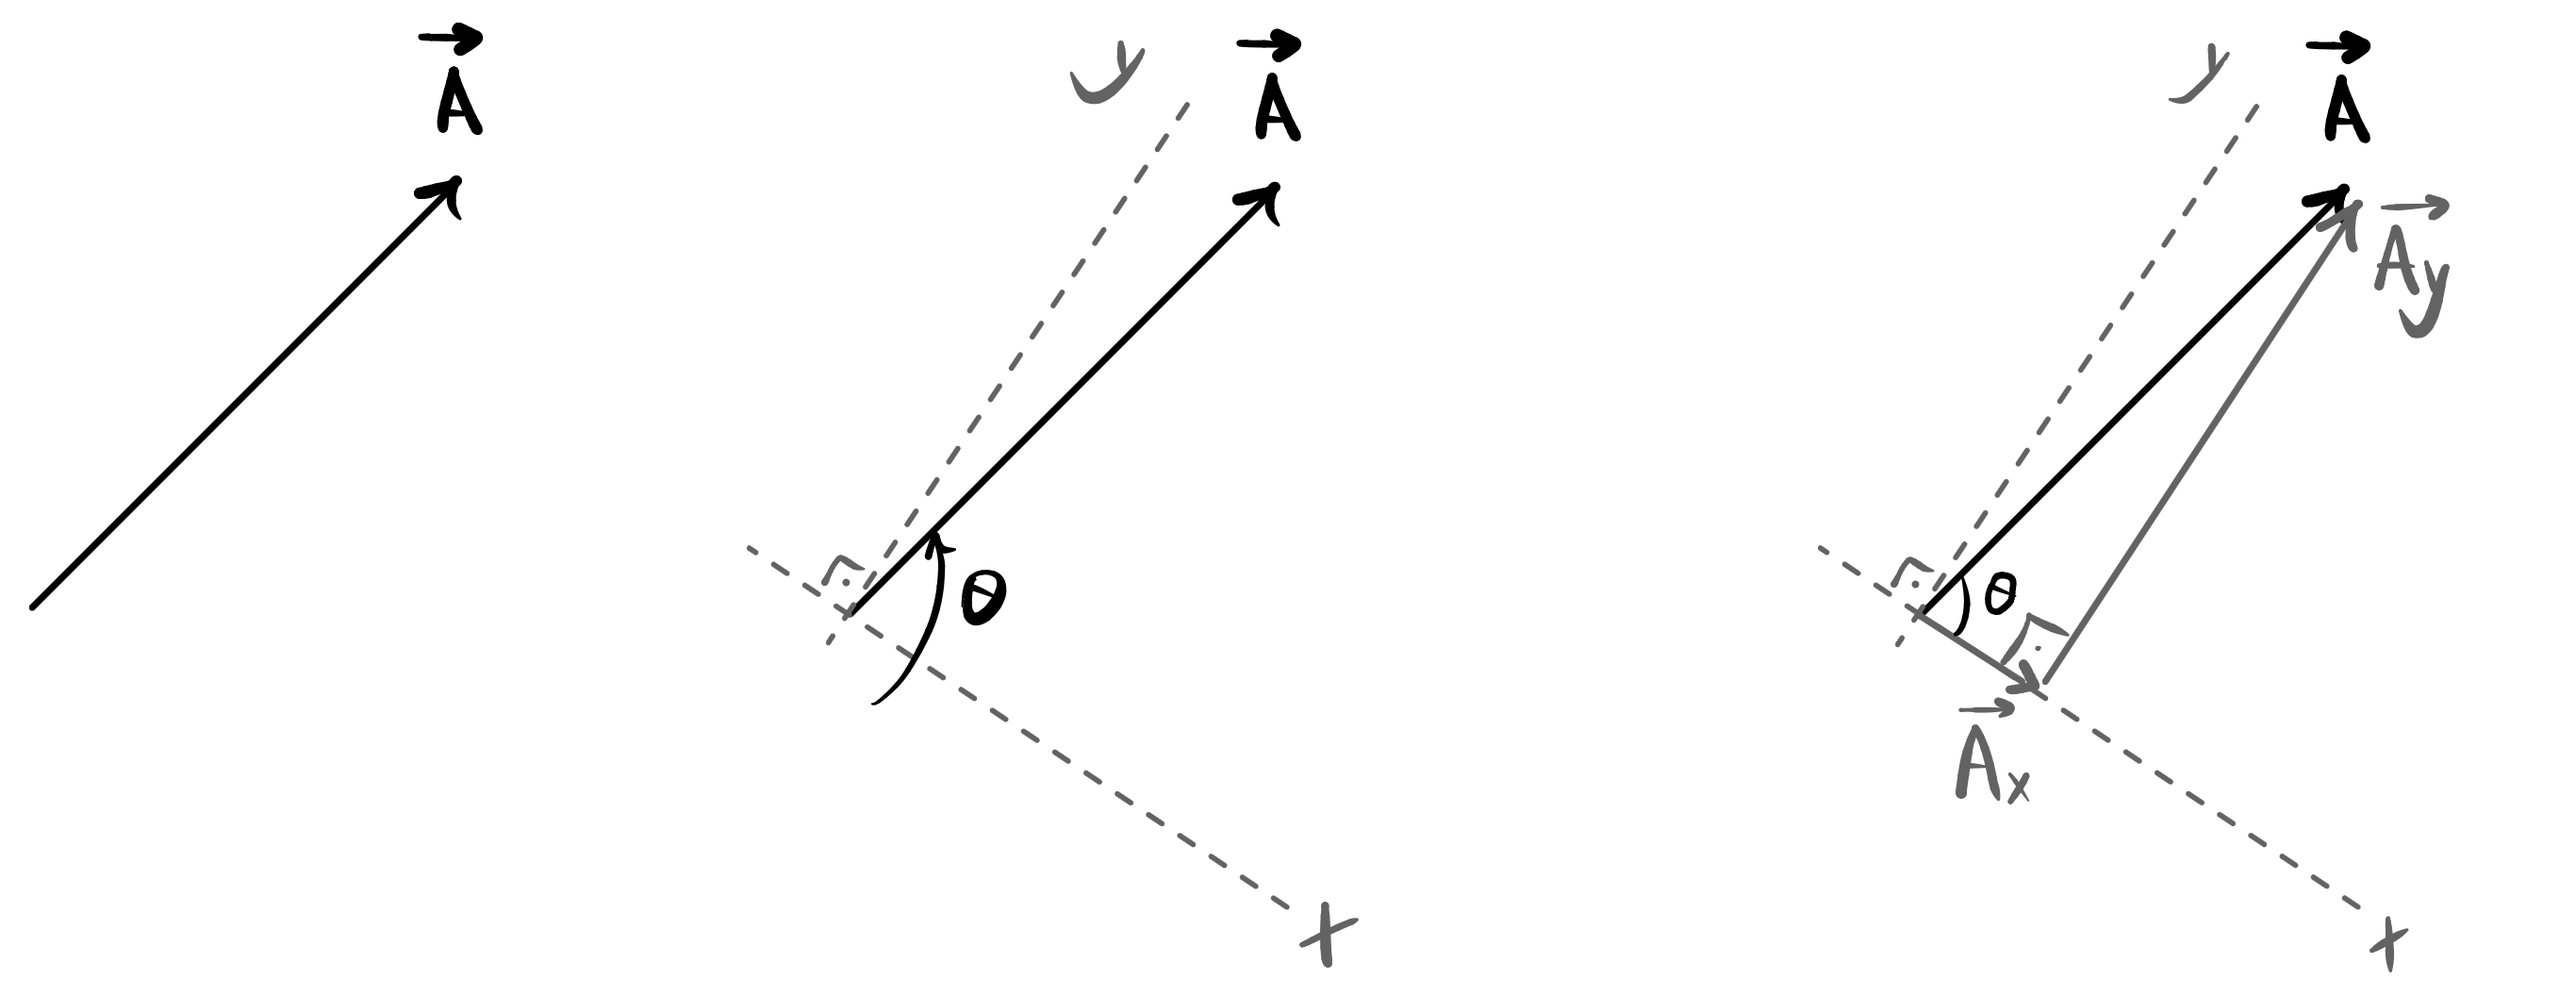
\includegraphics[scale=0.13]{imagenscinematicavetorial/decomporvetores2.jpeg}
    \caption{A decomposição vetorial nas direções perpendiculares quaisquer.}
    \label{fig_cinvet_decomporvetores2}
\end{figure}


Poderíamos ter escolhido quaisquer outras direções nas quais quiséssemos decompor o vetor inicial $\vec{A}.$ Tais direções sequer precisariam ser perpendiculares entre si -- mas nos ateremos sempre a estes casos, dadas as vantagens anteriormente mencionadas. Considere, por exemplo, a Figura \ref{fig_cinvet_decomporvetores2}, que contém o mesmo vetor $\vec{A}$, porém agora as direções perpendiculares $x$ e $y$ nas quais se pretende decompô-lo são outras. Note que o procedimento é exatamente o mesmo: ao projetar o vetor $\vec{A}$ em cada uma dessas direções teremos as suas componentes, o que aparece representado na terceira imagem da figura. Perceba que as mesmas relações de antes são válidas, isto é:

\begin{enumerate}
    \item [(i)] Os vetores $\vec{A}_x$ e $\vec{A}_y$, somados, resultam no vetor $\vec{A};$ ou seja, vale a equação vetorial:

    $$ \vec{A} = \vec{A}_x + \vec{A}_y. $$

    \item [(ii)] Os módulos das componentes $A_x$ e $A_y$ se relacionam com o módulo $A$ do vetor inicial pelo Teorema de Pitágoras \footnote{Isso sempre ocorrerá quando as direções $x$ e $y$ de decomposição forem perpendiculares, porque isso sempre fará com que o triângulo de vetores da terceira imagem das Figuras \ref{fig_cinvet_decomporvetores1} e \ref{fig_cinvet_decomporvetores2} seja um triângulo retângulo.}, de modo que vale a equação algébrica:

    $$ A^2 = A_x^2 + A_y^2.$$

    \item [(iii)] Os módulos das componentes $A_x$ e $A_y$ se relacionam com o módulo $A$ do vetor inicial e com o ângulo $\theta$ que ele faz com a direção $x$ por meio das equações

    $$ \boxed{A_y = A \sin \theta} \quad  \text{ e } \quad \boxed{A_x = A \cos \theta,}$$

    \noindent o que mudou, neste caso, foi apenas as direções de decomposição -- ou seja, o valor de $\theta$ -- de modo que as componentes nas novas direções $x$ e $y$ terão, naturalmente, valores distintos.
\end{enumerate}


\begin{figure}[h]
    \centering
    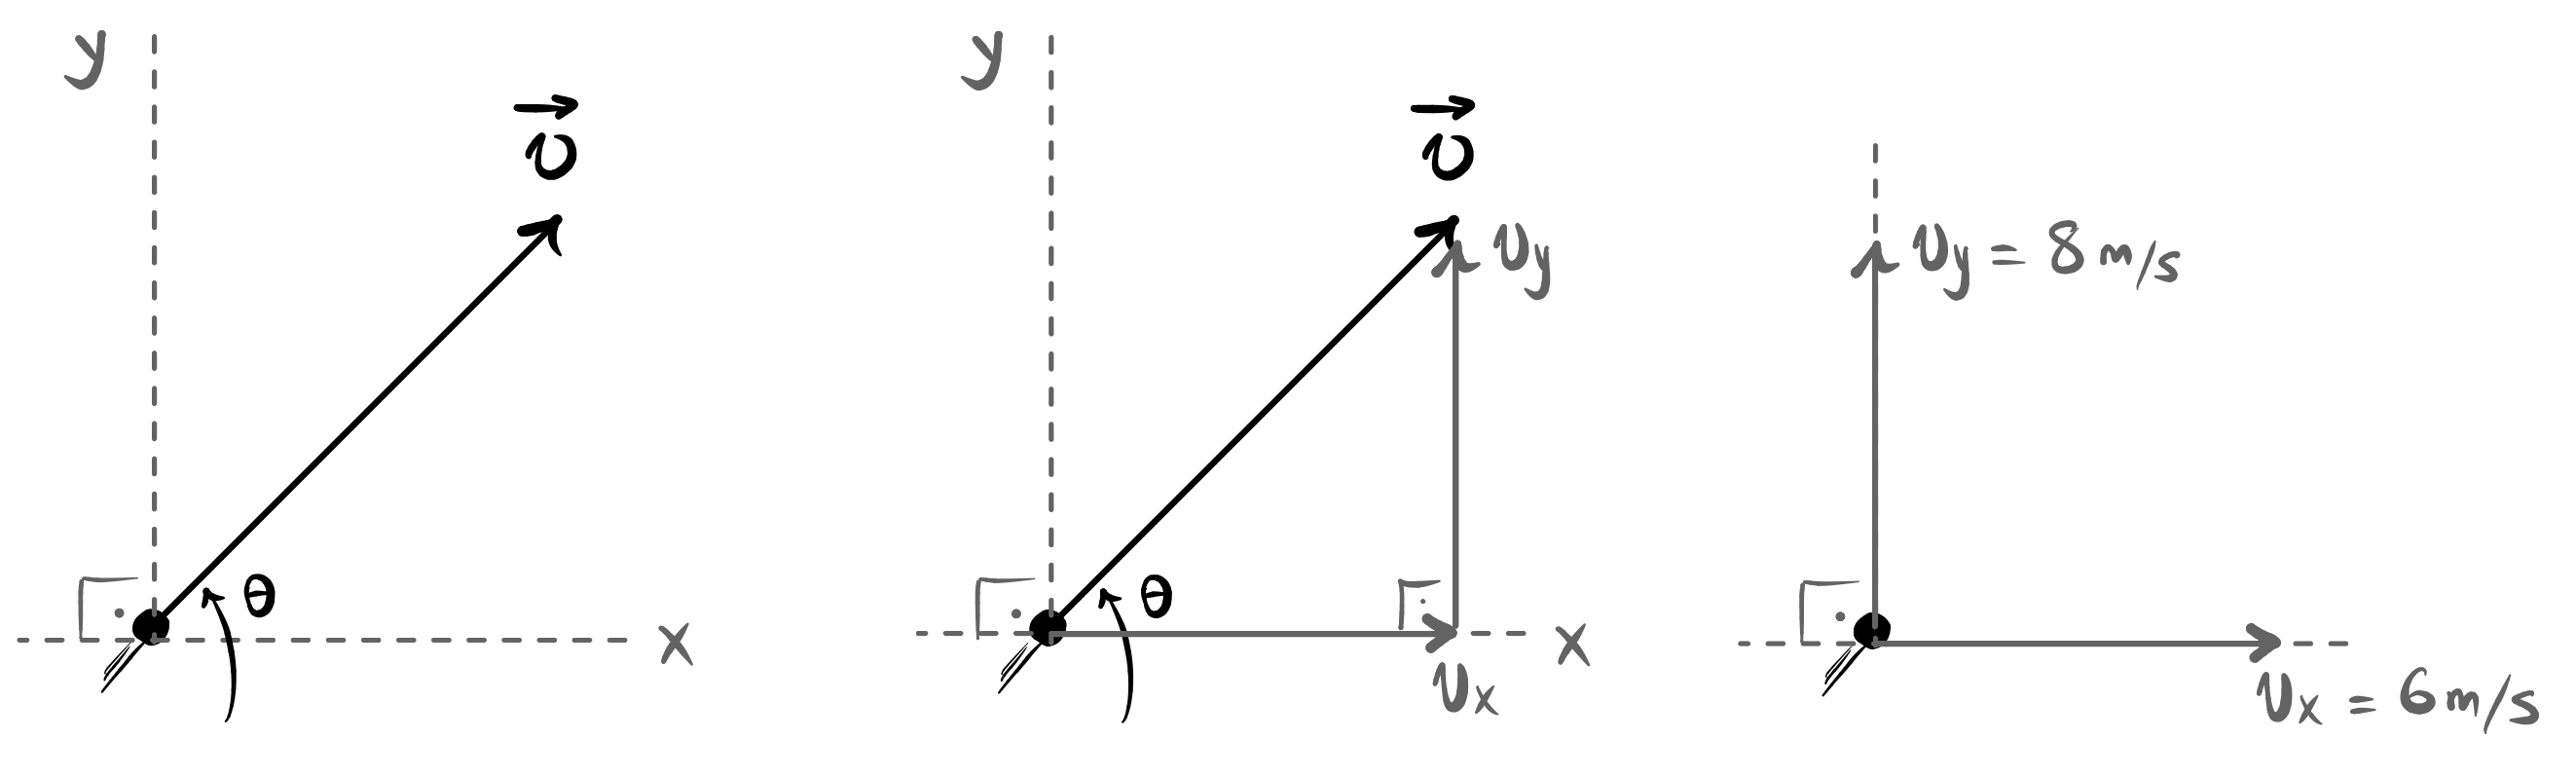
\includegraphics[scale=0.15]{imagenscinematicavetorial/decomporvetores3.jpeg}
    \caption{Fazendo uma decomposição vetorial.}
    \label{fig_cinvet_decomporvetores3}
\end{figure}


Para não deixar totalmente abstrata essa nova operação, avaliemos o caso da Figura \ref{fig_cinvet_decomporvetores3}, em que o ângulo $\theta$ com a direção $x$ é tal que $\sin \theta = 0.8$ e $\cos \theta = 0.6.$ Considere que trata-se de uma bola, que foi lançada com velocidade $v=10$ m/s, fazendo o ângulo $\theta$ em questão com a direção horizontal.





Podemos decompor tal velocidade nas direções $x$ e $y$, e suas componentes podem ser obtidas por meio das razões trigonométricas no triângulo retângulo da segunda imagem da figura:


\begin{align}
    \sin \theta &= \dfrac{v_y}{v} \implies v_y = v \sin \theta = 10 \cdot 0.8 \implies  \boxed{v_y=8 \text{ m/s,}} \nonumber \\
     \cos \theta &= \dfrac{v_x}{v} \implies v_x = v \cos \theta = 10 \cdot 0.6 \implies  \boxed{v_x=6 \text{ m/s.}} \nonumber
\end{align}

Perceba que $v_x^2+v_y^2=6^2+8^2=100=10^2=v^2,$ isto é, os módulos das componentes de velocidade se relacionam com o módulo da velocidade original por meio do Teorema de Pitágoras.

Logo, como os vetores $\vec{v}_x$ e $\vec{v}_y$ somados resultam no vetor inicial $\vec{v},$ em certa medida, lançar uma bola com velocidade $v=10$ m/s em uma direção que faz o ângulo $\theta$ em questão com a horizontal é o mesmo que lançá-la para cima com uma velocidade $v_y=8$ m/s e empurrá-la, ao mesmo tempo, para a direita, fornecendo-a uma velocidade horizontal $v_x=6$ m/s, como mostra a terceira imagem da Figura \ref{fig_cinvet_decomporvetores3}.

Isso será extremamente importante na Física: interpretar um movimento como sendo composto por dois movimentos independentes em duas direções perpendiculares; ou somar o efeito de dois movimentos em direções perpendiculares para obter o movimento composto.


\newpage




\section{Velocidade Vetorial}



\begin{secnivel}[Velocidade Vetorial Média]{I}{Velocidade Vetorial Média}
  
  \eqLdois{def}{cinvet_eq_velocidadevetorialmedia}{\vec{v}_m := \dfrac{\Delta \vec{r}}{\Delta t}}

\end{secnivel}




\secgfe{De onde vem}

Para acompanharmos um movimento bidimensional é comum adotarmos uma origem e localizarmos a partícula por meio de um vetor posição $\vec{r},$ que vai da origem até à posição atual da partícula. Note que isso é bem razoável: se você está acompanhando um passarinho voando, você o localiza por uma linha imaginária que vai dos seus olhos até o objeto em observação. Nesse sentido, os seus olhos seriam a origem do sistema de referência e essa linha pontilhada representa a direção do vetor posição, que aponta para o objeto observado.

Tal situação está representada na Figura \ref{fig_cinvet_vetorposicao01}, em que vetor posição $\vec{r}_1$ vai dos olhos do observador à partícula observada no instante $t_1,$ e o vetor posição $\vec{r}_2$ vai dos olhos do observador à partícula observada no instante $t_2$. O deslocamento vetorial $\Delta \vec{r}$ é definido, naturalmente, como sendo a variação da posição vetorial, ou seja:

$$ \Delta \vec{r} := \vec{r_2} - \vec{r_1},$$

\noindent e, como vimos, fazer essa subtração vetorial é somar o vetor $\vec{r}_2$ com o inverso do vetor $\vec{r}_1,$ o que aparece na segunda e terceira imagem da Figura \ref{fig_cinvet_vetorposicao01}, fornecendo o vetor deslocamento $\Delta \vec{r}$ como sendo o vetor que vai da posição inicial até a posição final.


\begin{figure}[h]
    \centering
    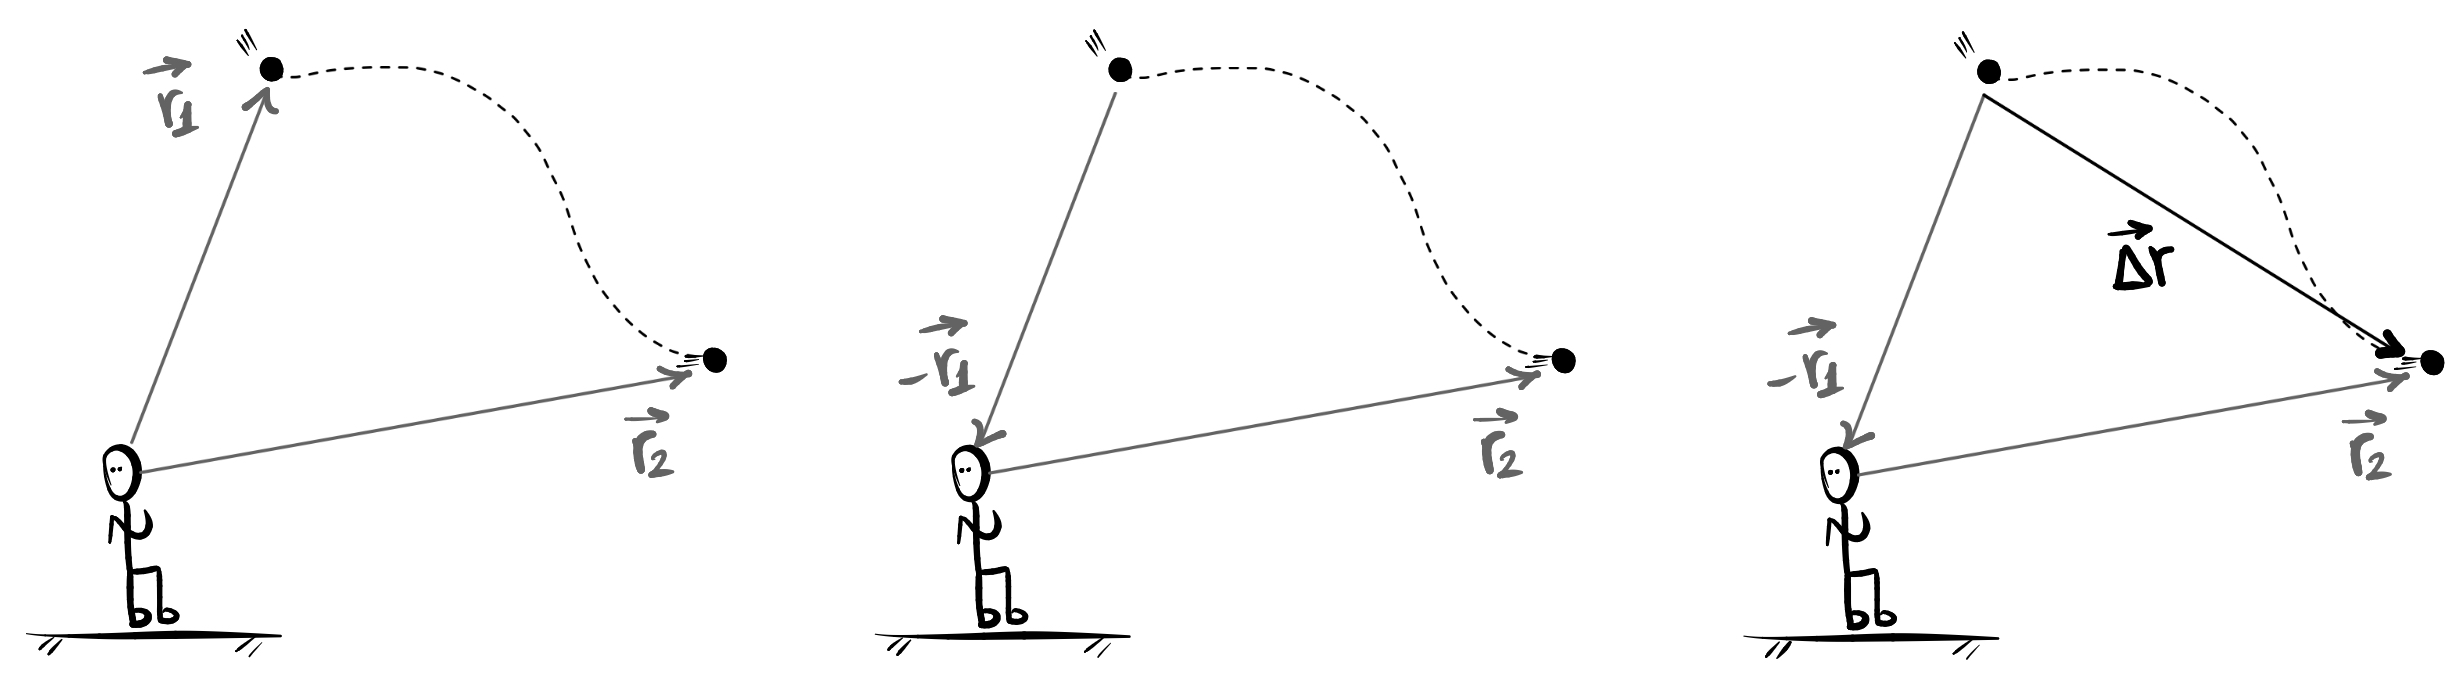
\includegraphics[scale=0.18]{imagenscinematicavetorial/vetorposicao.jpeg}
    \caption{O vetor posição $\vec{r}$ e o deslocamento vetorial $\Delta \vec{r}.$}
    \label{fig_cinvet_vetorposicao01}
\end{figure}

Vale notar que, apesar dos vetores posição $\vec{r}_1$ e $\vec{r}_2$ serem diferentes para diferentes observadores -- ou seja, a posição de um certo objeto no tempo depende do referencial --, o vetor deslocamento é algo absoluto, que não depende do referencial. Isso pode ser notado pela Figura \ref{fig_cinvet_vetorposicao02}, que mostra o mesmo movimento sendo analisado por um observador distinto. Note que os vetores posição $\vec{r}_1$ e $\vec{r}_2$ são diferentes daqueles do referencial da Figura \ref{fig_cinvet_vetorposicao01}; já o vetor deslocamento $\Delta \vec{r}$ é exatamente o mesmo: ele vai da posição inicial até a posição final do objeto.\footnote{O vetor deslocamento será sempre o mesmo para observadores em repouso, naturalmente. Um observador em movimento perceberia um deslocamento distinto.}


\begin{figure}[h]
    \centering
    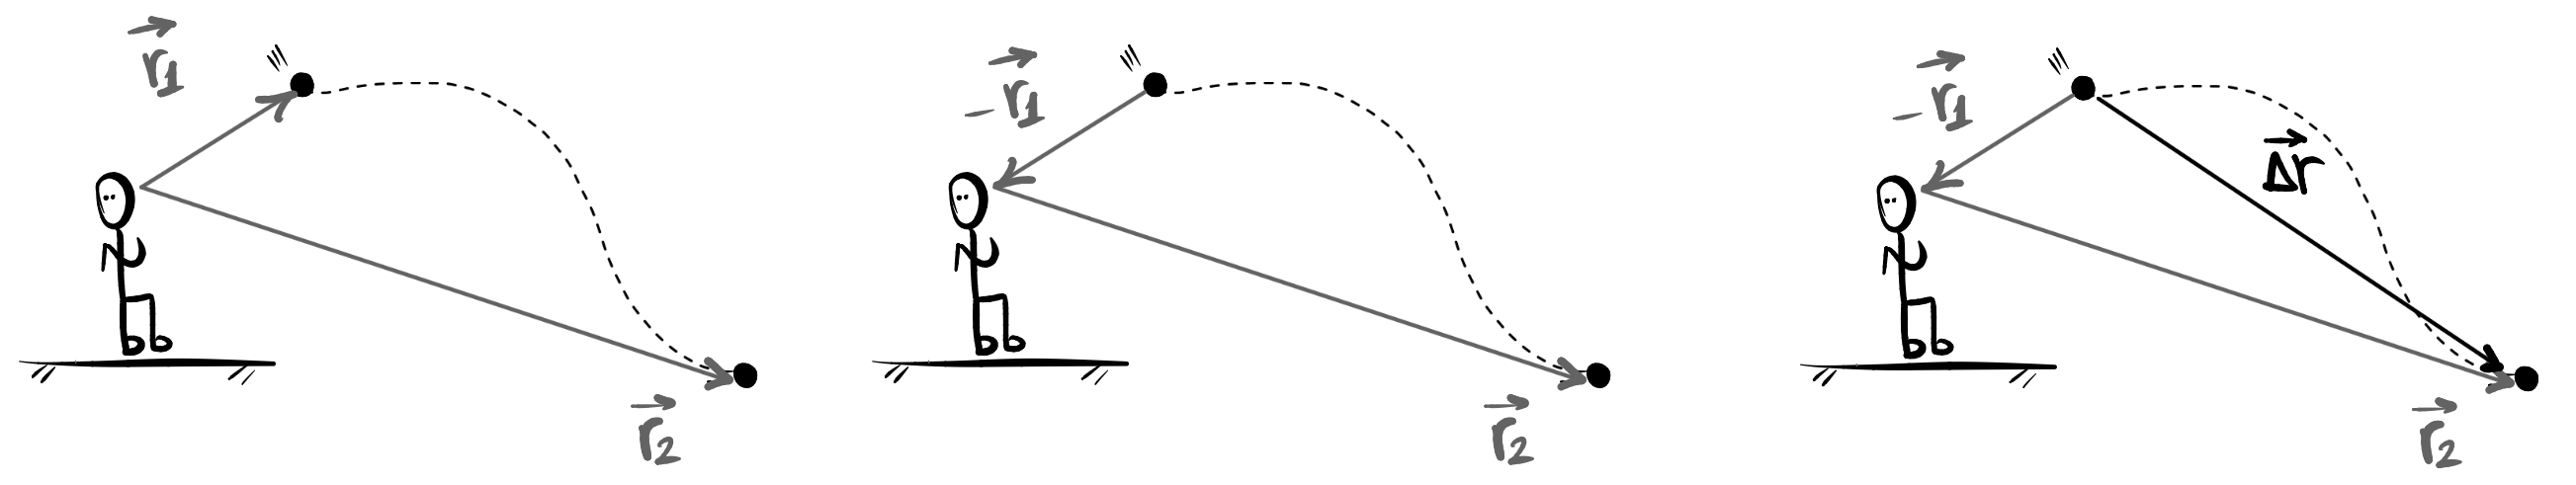
\includegraphics[scale=0.18]{imagenscinematicavetorial/vetorposicao02.jpeg}
    \caption{O vetor deslocamento $\Delta \vec{r}$ visto por um outro referencial em repouso.}
    \label{fig_cinvet_vetorposicao02}
\end{figure}


A Figura \ref{fig_cinvet_deslocamentoedistancia} dá um destaque para o deslocamento do corpo e a sua trajetória, removendo os observadores e os vetores posição, haja vista que o deslocamento e distância são os mesmos, independente do sistema de referência -- desde que ele esteja em repouso. Vale destacar, novamente, a diferença entre as duas grandezas: a distância percorrida mede o comprimento da trajetória do corpo, enquanto o deslocamento mede a distância entre suas posições inicial e final. É importante perceber essa diferença porque, como veremos, existirá uma situação muito importante na qual as duas grandezas irão coincidir -- e essa é a grande razão de definirmos a velocidade vetorial média como o fizemos.



\begin{figure}[h]
    \centering
    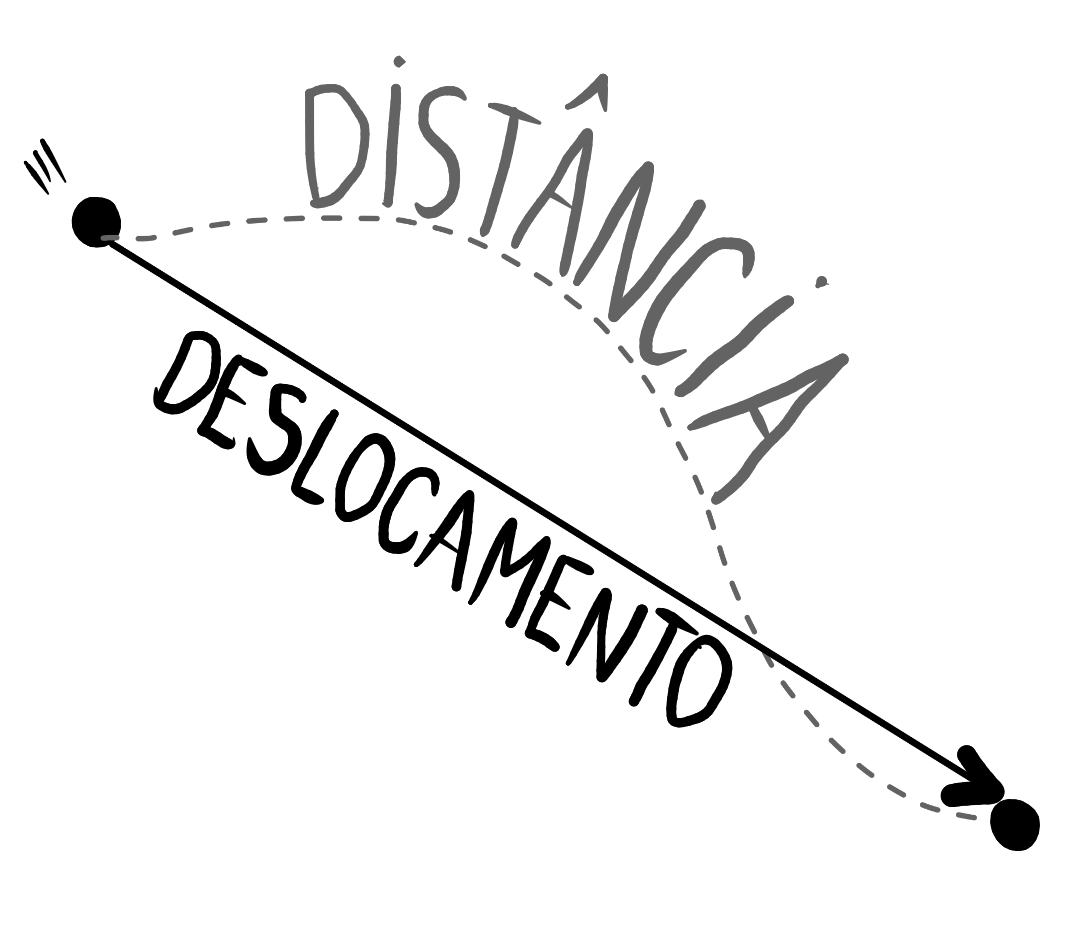
\includegraphics[scale=0.12]{imagenscinematicavetorial/vetordeslocamentoedistancia.jpeg}
    \caption{O vetor deslocamento $\Delta \vec{r}$ e a distância percorrida.}
    \label{fig_cinvet_deslocamentoedistancia}
\end{figure}

Feita essa digressão, definimos a velocidade vetorial média $\vec{v}_m$ como sendo a razão entre o deslocamento vetorial e o intervalo de tempo no qual ele se deu, ou seja:

 $$ \vec{v}_m :=\dfrac{\Delta \vec{r}}{\Delta t}.$$

 Perceba que tal definição é razoável, e não é lá tão diferente de como definimos a velocidade escalar média pela Equação \eqref{mecanica_eq_velocidademedia}, exceto pelo fato de que, aqui, incorporamos na equação o caráter vetorial da velocidade, o que nos possibilitará descrever movimentos em mais de uma dimensão, como havíamos discutido. A Figura \ref{fig_mec_deslocamento_vs_distancia02cinv} ilustra um movimento desse tipo, destacando a diferença entre a distância percorrida e o deslocamento vetorial. Vale ressaltar que, em movimentos nos quais o corpo retorna à posição de origem, o deslocamento vetorial é nulo ainda que a distância percorrida não o seja.

 \begin{figure}[h]
    \centering
    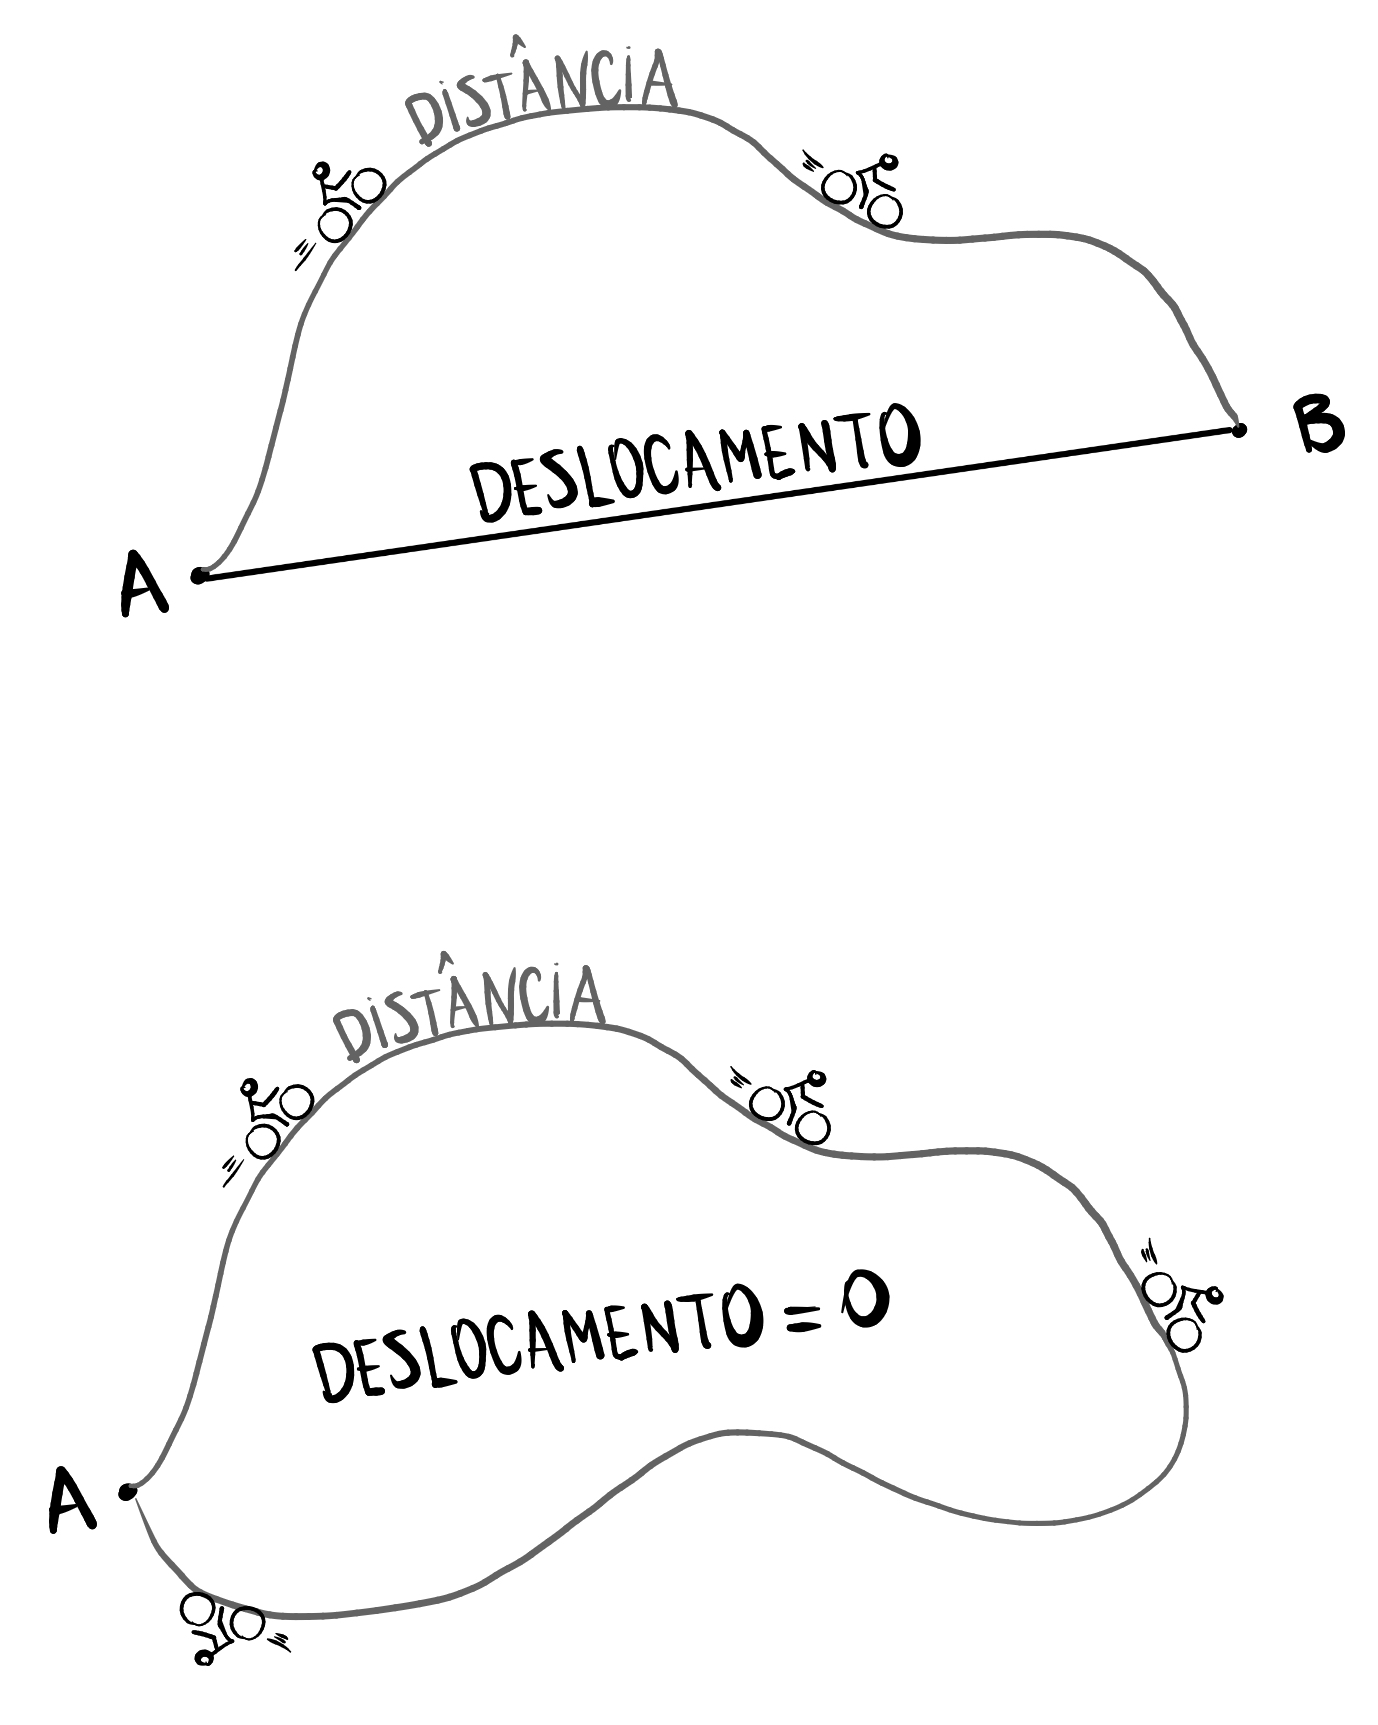
\includegraphics[scale=0.13]{imagensmecanica/deslocamentovsdistancia02.jpeg}
    \caption{A diferença entre o deslocamento $|\Delta \vec{r}|$ e a distância percorrida $d$.}
    \label{fig_mec_deslocamento_vs_distancia02cinv}
\end{figure}


Pela definição feita, o vetor velocidade média $\vec{v}_m$ é basicamente o vetor deslocamento $\Delta \vec{r}$ multiplicado por um escalar, isto é, o número real $\sfrac{1}{\Delta t}$. E, como o intervalo de tempo é sempre positivo, tal número será sempre positivo, de modo que o vetor $\vec{v}_m$, sendo um múltiplo positivo do vetor $\Delta \vec{r}$, apontará sempre na mesma direção e sentido deste. Logo, para uma partícula em movimento, seu vetor velocidade média sempre apontará na direção que une a posição inicial à posição final, apontando no sentido da posição inicial para a posição final.
 

 

\secgfe{Onde é usada}

A verdade é que é bastante raro usarmos diretamente a Equação \eqref{cinvet_eq_velocidadevetorialmedia}. Faremos, em breve, alguns exemplos, de modo que ficará claro para o leitor como ele pode precisar usar tal equação em certos problemas. Contudo, já adianto que tais exemplos são um pouco artificiais e é pouco provável que o leitor precise fazer cálculos como estes em algum momento.

Dito isso, por qual razão, então, estudamos tal equação? Como veremos em breve, o mais importante não é a fórmula e o uso dela em si, mas sim uma consequência que está contida, implicitamente, dentro dela. Tal consequência é tão importante que dedicaremos um espaço exclusivo para ela, nas \textbf{observações} sobre essa equação.




\secgfe{Erros comuns}

Novamente, o erro mais comum aqui é confundir distância com deslocamento. Note que, na Equação \eqref{cinvet_eq_velocidadevetorialmedia}, o que entra no numerador é o deslocamento, e não a distância percorrida.



\secgfe{Observações}


Como levantado anteriormente, existe uma consequência importante, que diz algo extremamente relevante a respeito da velocidade de um corpo, e está contida na forma como definimos a Equação \eqref{cinvet_eq_velocidadevetorialmedia}. Note que tal equação define o vetor \textbf{velocidade média $\vec{v}_m$} de um corpo entre dois instantes, digamos $t_1$ e $t_2$. Veja o que acontece quando fazemos o instante $t_2$ ser muito próximo do instante $t_1$, ou seja, o intervalo $\Delta t$ em que analisamos o movimento passa a ser cada vez mais curto. 



\begin{figure}[h]
    \centering
    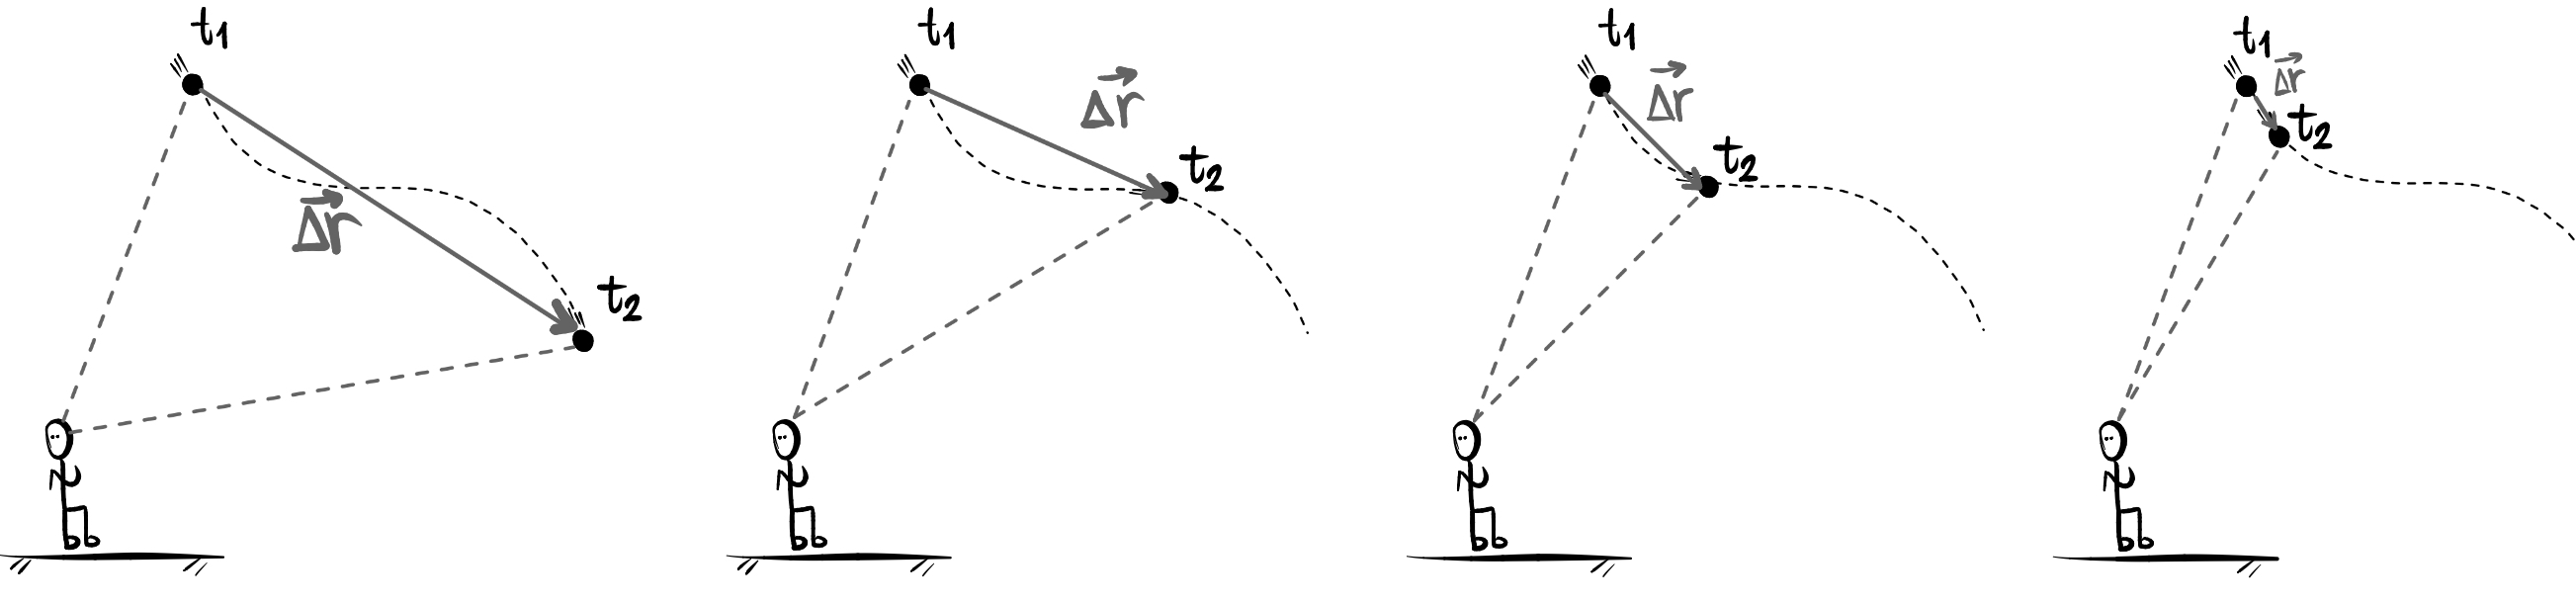
\includegraphics[scale=0.20]{imagenscinematicavetorial/deltatpequeno.jpeg}
    \caption{O vetor deslocamento $\Delta \vec{r}$ avaliado em um intervalo de tempo cada vez menor.}
    \label{fig_cinvet_deltatpequeno}
\end{figure}

Isso aparece na Figura \ref{fig_cinvet_deltatpequeno}, em que estudamos o mesmo movimento, porém analisado em um intervalo de tempo cada vez mais curto. As linhas pontilhadas saindo dos olhos do observador representariam as direções dos vetores posição inicial e final -- o que sequer é relevante, haja vista que o deslocamento sempre apontará da posição inicial do objeto para a sua posição final, mas preferimos deixar tais segmentos de marcação.

Digamos, para fins didáticos, que o intervalo de tempo inicial é $\Delta t = t_2-t_1 = 1 $s. Na segunda imagem da figura, digamos que reduzimos tal intervalo para $\Delta t = t_2-t_1 = 0.1 $s, e na terceira imagem, para $\Delta t = t_2-t_1 = 0.01 $s. Na quarta imagem, digamos que o intervalo de tempo analisado foi de um milésimo de segundo, ou seja, $\Delta t = t_2-t_1 = 0.001 $s.






Perceba que, à medida que o intervalo de tempo fica cada vez mais curto\footnote{Neste caso, o intervalo $\Delta t = t_2-t_1$ está diminuindo porque estamos fazendo $t_2$ se tornar cada vez mais próximo de $t_1.$ O instante $t_1,$ por sua vez, está sendo considerado fixo.}, duas coisas importantes acontecem:

\begin{enumerate}
    \item [(i)] A velocidade média calculada entre os instantes $t_1$ e $t_2$ fica cada vez mais próxima da velocidade instantânea da partícula no instante $t_1,$ isto é, sua velocidade exata em $t_1$, uma vez que a média é feita em um intervalo de tempo tão curto que praticamente não dá tempo de a velocidade variar substancialmente.
    
    \item [(ii)] Quando o intervalo de tempo fica realmente muito pequeno, como é o caso de avaliar para um milésimo de segundo, na última imagem da Figura \ref{fig_cinvet_deltatpequeno}, o módulo do vetor deslocamento $\Delta \vec{r}$ coincide com a distância percorrida $d$ e se torna \textbf{tangente à trajetória.} Este fato é tão importante que merece uma atenção própria: a Figura \ref{fig_cinvet_deslocamentoedistanciazoom} mostra um zoom na situação do intervalo de tempo de um milésimo de segundo -- a última situação da Figura \ref{fig_cinvet_deltatpequeno}. \\


\begin{figure}[h]
    \centering
    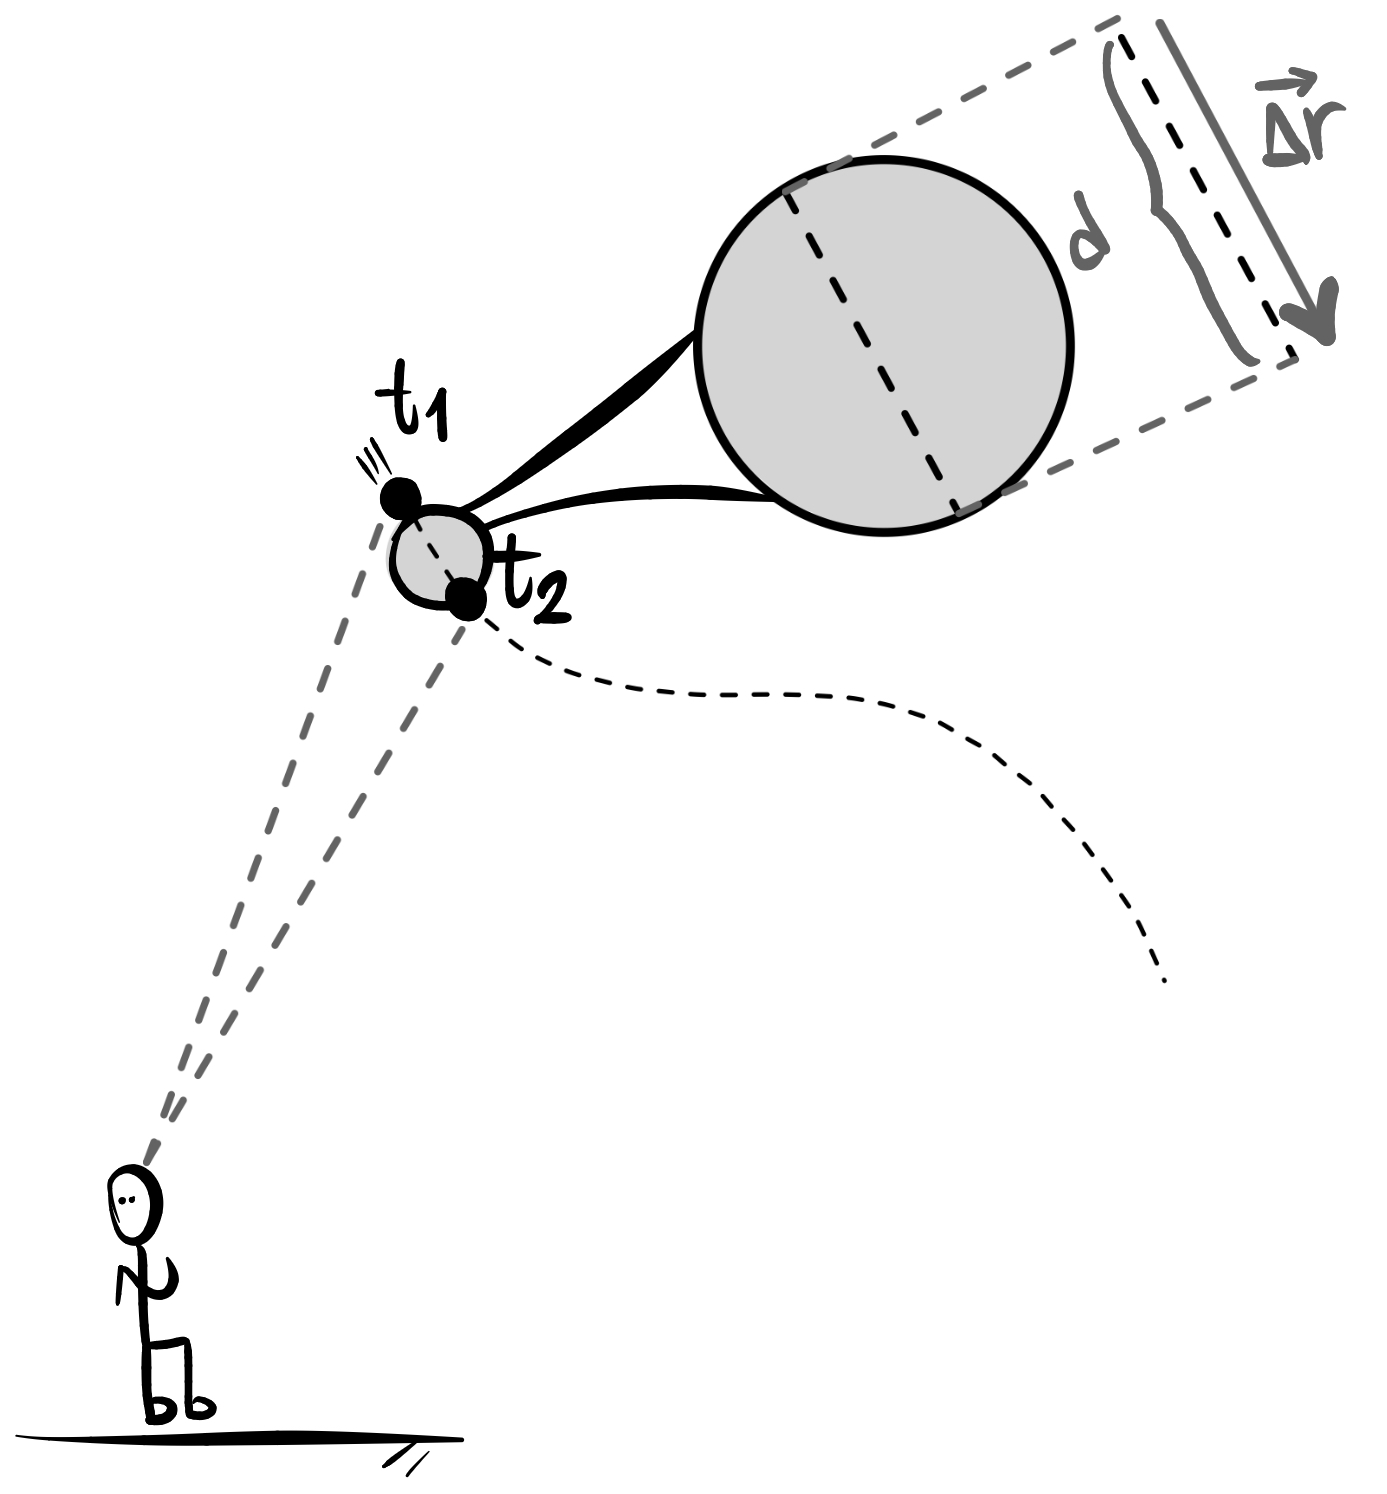
\includegraphics[scale=0.12]{imagenscinematicavetorial/zoomdeltaredistancia.jpeg}
    \caption{O módulo do vetor deslocamento $\Delta \vec{r}$ coincide com a distância percorrida $d$ para intervalos de tempo muito curtos.}
    \label{fig_cinvet_deslocamentoedistanciazoom}
\end{figure}
  
     Perceba que, por mais curvilíneo e esquisito que possa ser um movimento, em um intervalo de tempo suficientemente pequeno, ele se aproxima de uma reta.\footnote{Isso ocorre porque, sendo o tempo suficientemente pequeno -- pense em algo como um milésimo de um centésimo de um bilionésimo de segundo -- praticamente não deu tempo de o corpo se mover, seja para fazer uma curva ou se afastar substancialmente da posição inicial.} Desse modo, o deslocamento vetorial $\Delta \vec{r}$ -- que é a distância em linha reta da posição final à inicial -- coincide com a distância percorrida $d$, e a velocidade vetorial média instantânea $\vec{v}$ tem a direção da tangente à curva naquele ponto, apontando para o sentido do movimento.

     Daqui extraímos a \textbf{conclusão mais importante} de definirmos a velocidade vetorial média da forma como fizemos na Equação \eqref{cinvet_eq_velocidadevetorialmedia}: para uma partícula em um movimento qualquer, a sua velocidade vetorial $\vec{v}$, em cada instante,\footnote{Para que fique absolutamente claro este ponto, estamos falando da velocidade em cada instante porque, se fizermos a velocidade média entre $t_1=2.000$s e $t_2=2.001$s, o leitor há de concordar que tal valor será praticamente igual à velocidade da partícula no instante $t_1=2.000$s, uma vez que passou tão pouco tempo que a mudança na velocidade deve ter sido ínfima.} é tangente à sua trajetória e o seu módulo, naquele instante, coincide com o módulo da velocidade escalar média.

     
     A última parte da conclusão se refere ao fato de que, como distância e deslocamento coincidem, as razões
     
     
     $$ \dfrac{d}{\Delta t} \quad \text{e} \quad \dfrac{|\Delta \vec{r}|}{\Delta t}$$

     \noindent fornecerão exatamente o mesmo valor.
     

    
\end{enumerate}

Como dito, a parte mais importante do estudo da Equação \eqref{cinvet_eq_velocidadevetorialmedia} não é a aplicação da equação em si, mas sim uma informação que está contida implicitamente nela. Tal informação aparece ilustrada na Figura \ref{fig_cinvet_velocidadetangente} -- agora, para qualquer tipo de movimento bidimensional, o leitor já sabe exatamente qual é a propriedade geométrica que a velocidade do corpo em movimento deve satisfazer em todos os instantes: ela é sempre tangente à trajetória, apontando no mesmo sentido em que o movimento se dá.


\begin{figure}[h]
    \centering
    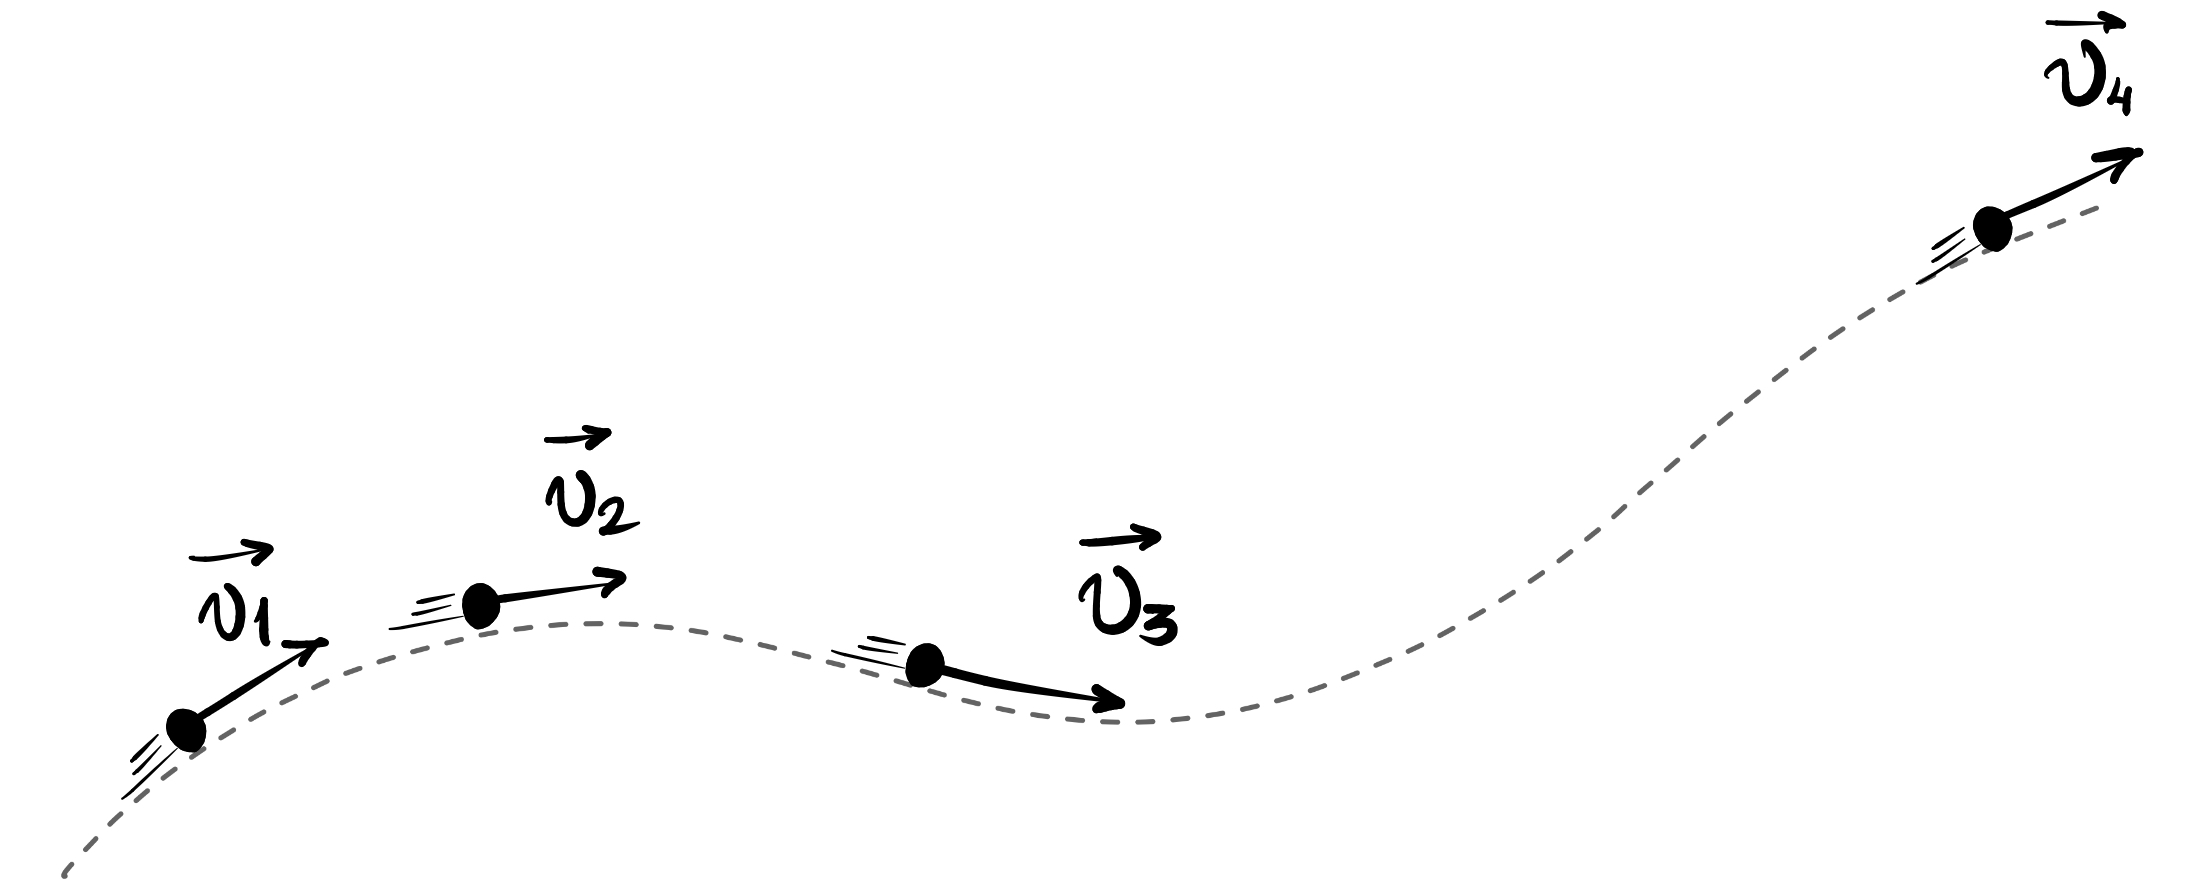
\includegraphics[scale=0.12]{imagenscinematicavetorial/velocidadetangente.jpeg}
    \caption{A velocidade vetorial $\vec{v}$ de uma partícula em movimento é sempre tangente à sua trajetória.}
    \label{fig_cinvet_velocidadetangente}
\end{figure}
  
É deste fato que decorre o fenômeno de \textit{sair pela tangente}. A velocidade aponta na direção e sentido para a qual o movimento tende a acontecer. Desse modo, na ausência de quaisquer forças ou interferências, um corpo sempre irá se mover exatamente na mesma direção e sentido para a qual aponta a sua velocidade. Considere o caso de uma pedra, amarrada por um barbante, que é posto a girar em torno de um centro fixo. Tal situação é a que aparece no primeiro desenho da Figura \ref{fig_cinvet_sairpelatangente}.


\begin{figure}[h]
    \centering
    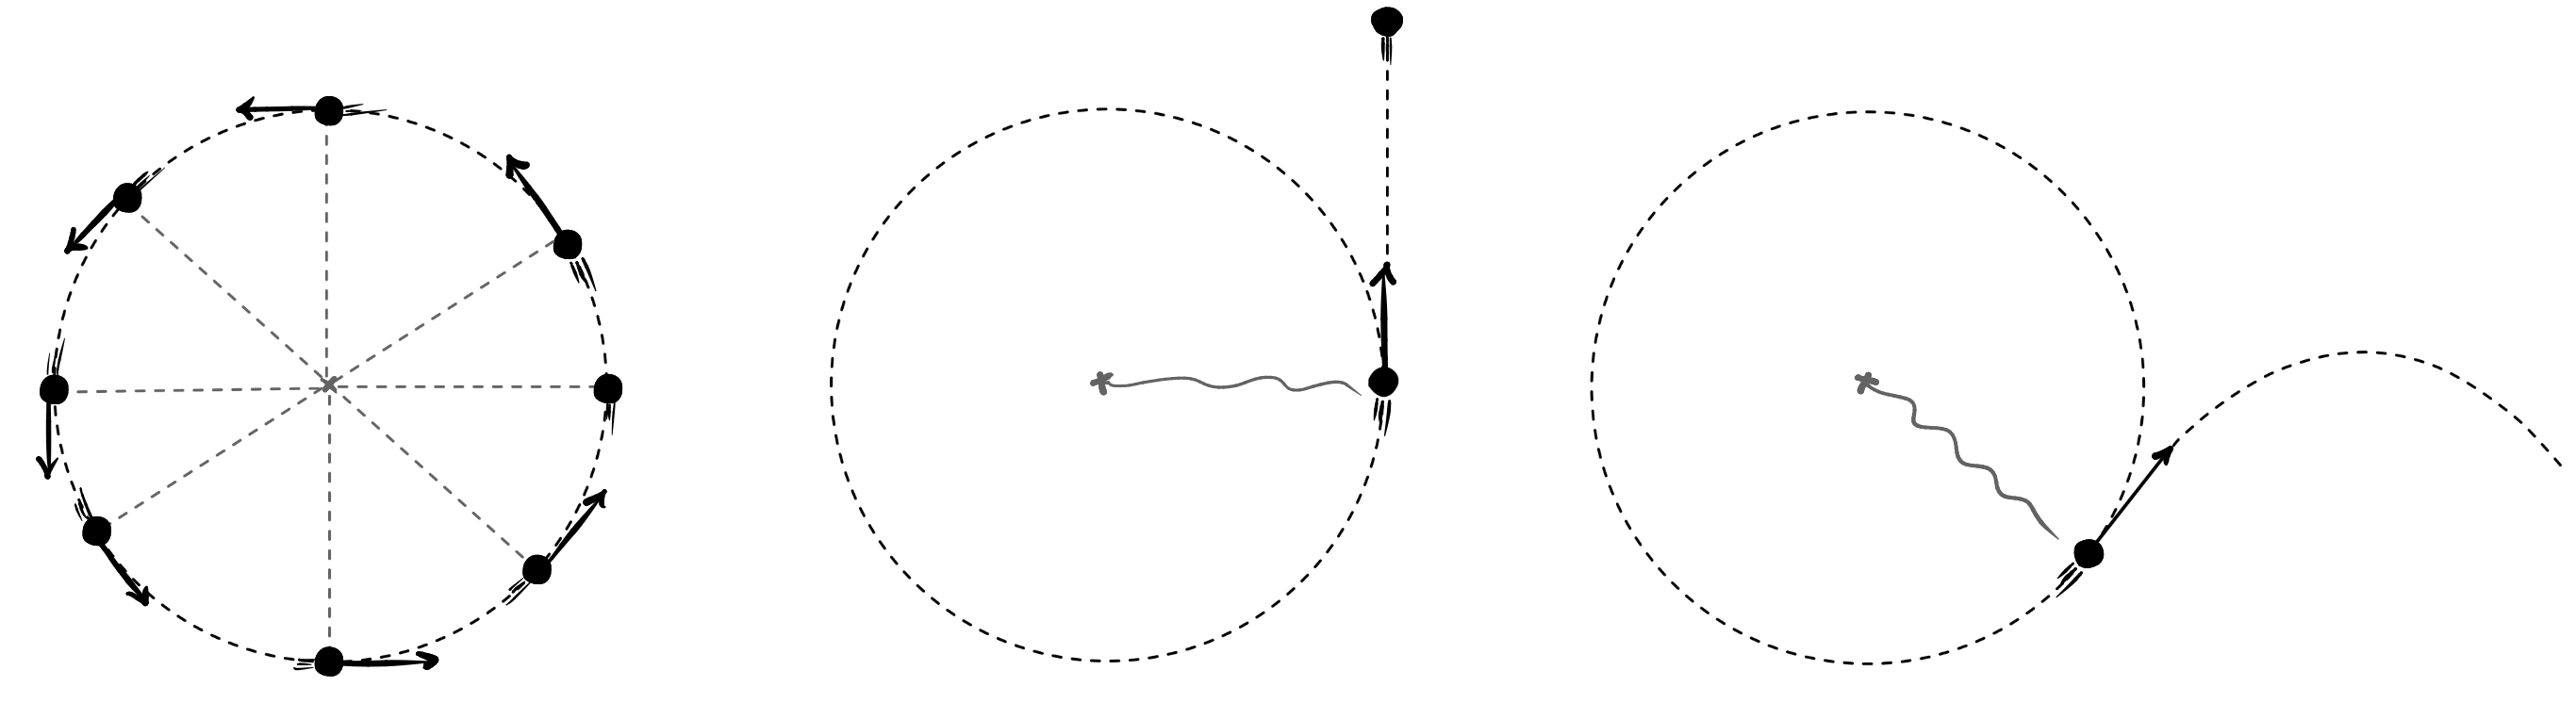
\includegraphics[scale=0.15]{imagenscinematicavetorial/sairpelatangente.jpeg}
    \caption{A velocidade vetorial $\vec{v}$ aponta na direção e sentido para onde o movimento se dá.}
    \label{fig_cinvet_sairpelatangente}
\end{figure}

Como já sabemos, em cada ponto a velocidade será tangente à trajetória. A pedra só não se move diretamente em tal direção porque existe uma força -- associada à sua conexão com o barbante -- que a confina e a obriga a se mover na trajetória circular. Contudo, se em qualquer ponto o barbante se romper, a partícula se moverá exatamente na direção para onde aponta a sua velocidade -- ela sairá na direção da tangente à circunferência, uma vez que a velocidade é tangente à circunferência. Tais situações estão ilustradas nas duas próximas imagens da Figura \ref{fig_cinvet_sairpelatangente}, que considera o barbante se rompendo para a pedra em duas posições diferentes. \footnote{Note que, no terceiro desenho da figura, a bolinha sai exatamente na direção da tangente. Sua trajetória, contudo, não é uma linha reta nessa direção devido à ação da gravidade, que puxa a bolinha para baixo, afetando e alterando a sua trajetória ao longo do movimento.}

\vspace{0.3cm}

%Exemplo resolvido

\begin{exemplo}[Nível I]\label{exemplo_cinematicavetorial_velocidadevetorialex01}

Um objeto sofre os sucessivos deslocamentos representados na Figura \ref{fig_cinvet_velocidadevetorialexemplo01}. Se o movimento todo dura $74$s, encontre seu vetor velocidade média ao longo de todo o intervalo -- ou seja, encontre seu módulo, direção e sentido.\\

Considere $\sin \theta = 0,8$ e $\cos \theta = 0,6.$

{
\centering
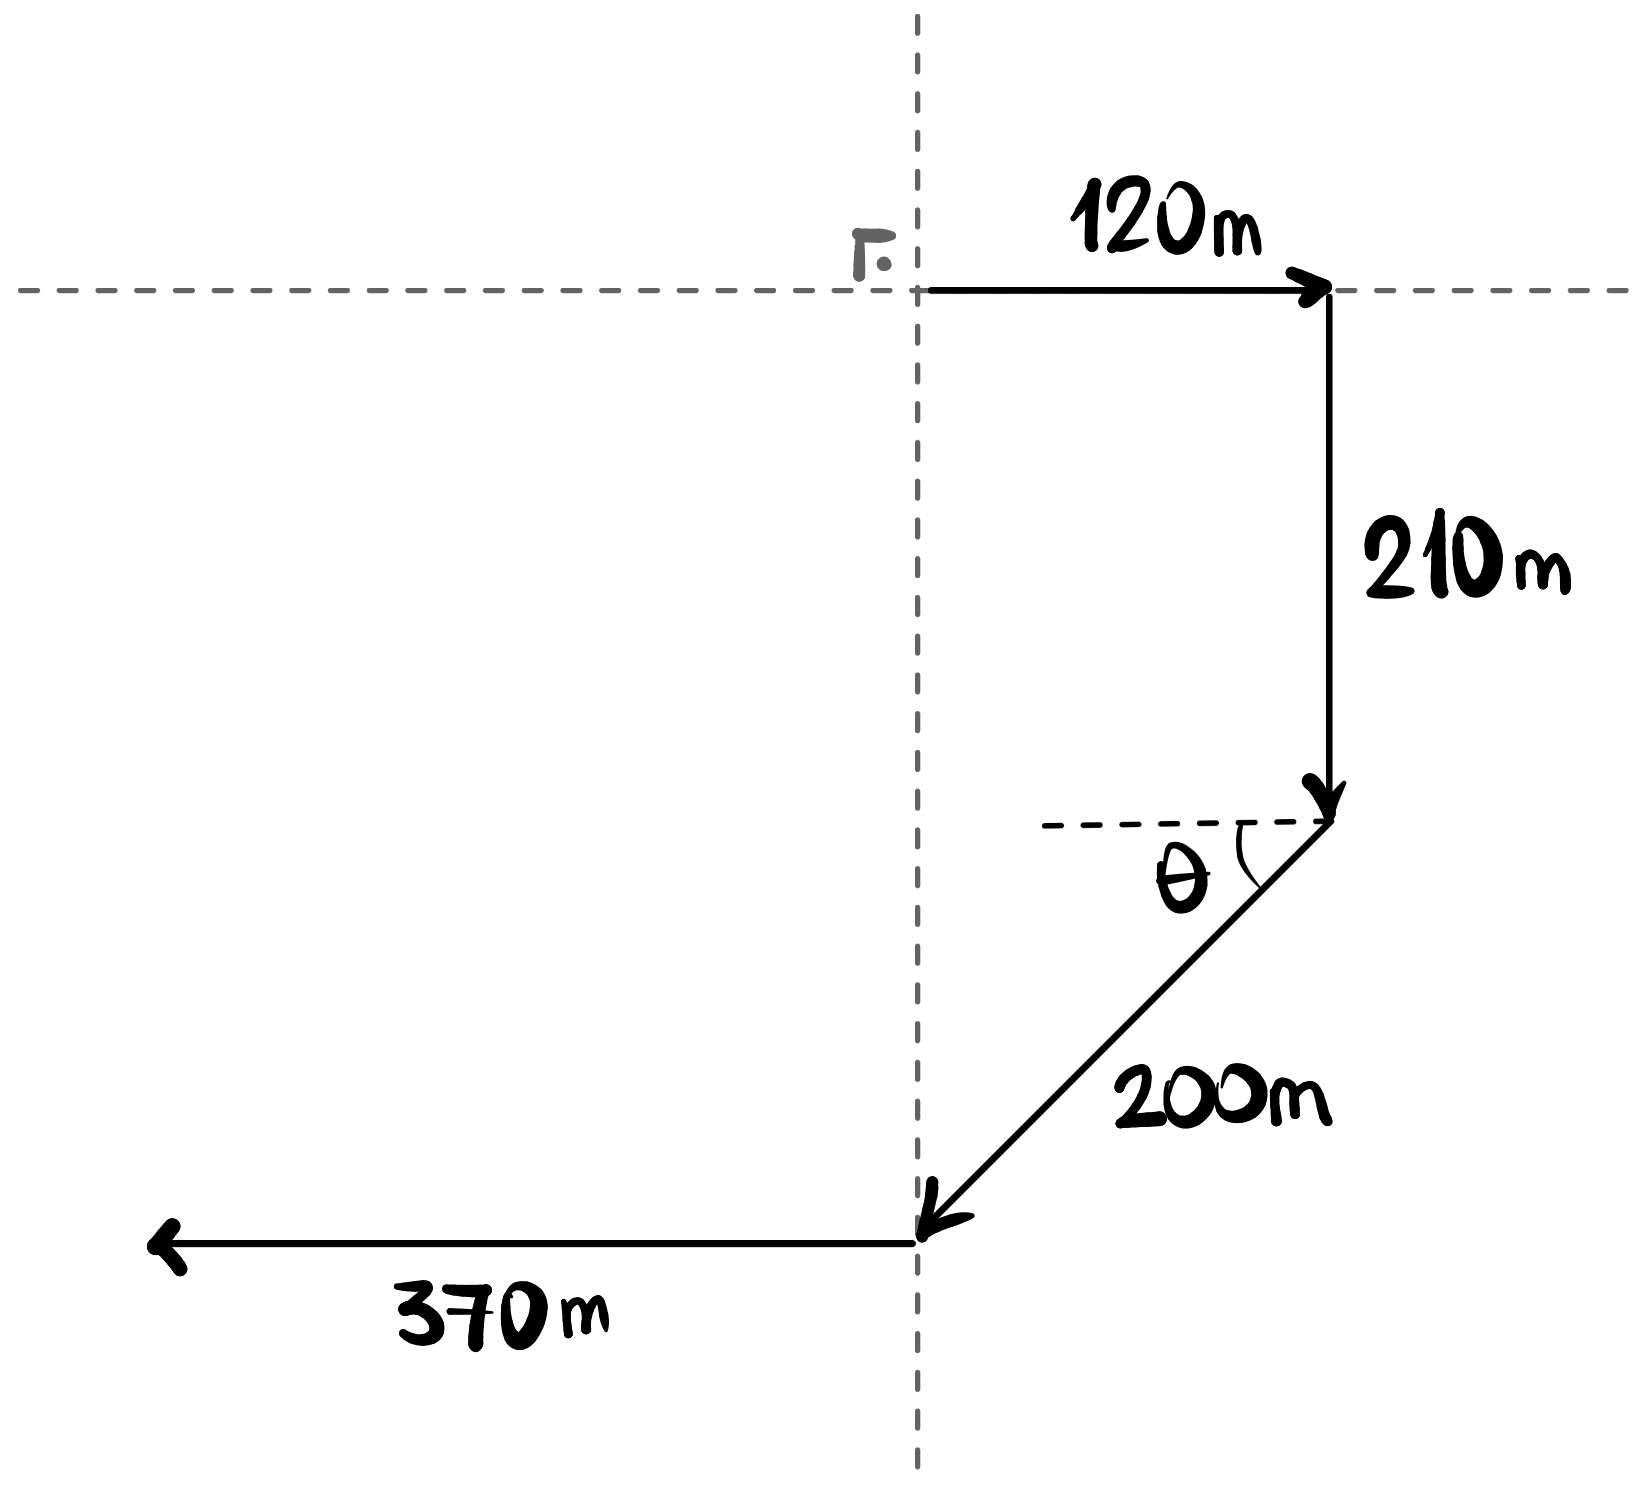
\includegraphics[width=0.3\linewidth]{imagenscinematicavetorial/velocidadevetorialexemplo1.jpeg}
\captionof{figure}{}
\label{fig_cinvet_velocidadevetorialexemplo01}
} 

\resolucao

Como mostra a primeira imagem da Figura \ref{fig_cinvet_velocidadevetorialexemplo0102}, sejam $a$ e $b$ os deslocamentos horizontal e vertical, respectivamente, oriundos do deslocamento inclinado de $200$ m. Podemos obter tais deslocamentos por meio de trigonometria básica:

$$ \sin \theta = \dfrac{b}{200} = 0.8 \implies \boxed{b=160 \text{ m}} \quad \text{e} \quad \cos \theta = \dfrac{a}{200} = 0.6 \implies \boxed{a=120 \text{ m.}}$$


{
\centering
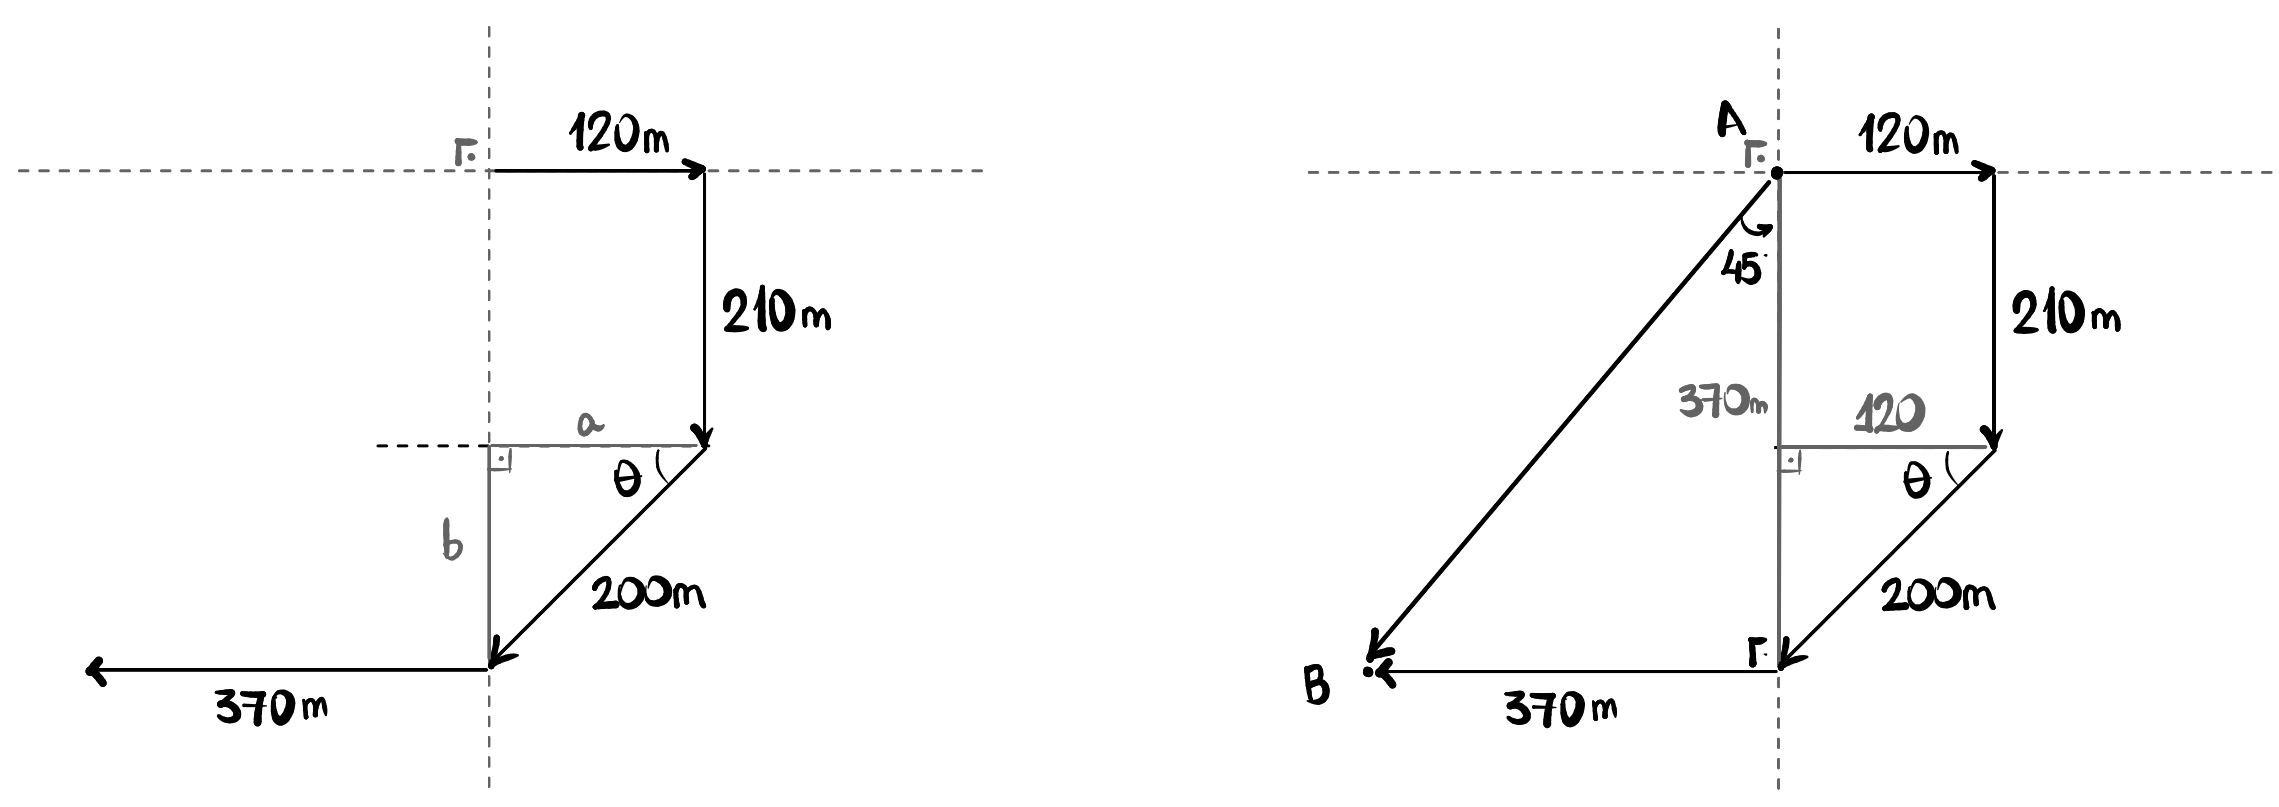
\includegraphics[width=0.8\linewidth]{imagenscinematicavetorial/velocidavetorialexemplo0102.jpeg}
\captionof{figure}{}
\label{fig_cinvet_velocidadevetorialexemplo0102}
} 

Com isso, podemos entender o vetor deslocamento de $200$m inclinado de $\theta$ como sendo composto por um deslocamento horizontal para a esquerda de $120$m --- que faz a partícula retornar ao alinhamento vertical inicial --- seguido de um deslocamento vertical para baixo de $160$m. Logo, o deslocamento vertical total é de $210+160=370$m, o que aparece na segunda imagem da Figura \ref{fig_cinvet_velocidadevetorialexemplo0102}. \\

Assim, o vetor deslocamento total $\Delta \vec{r}$ vai da posição inicial $A$ à posição final $B$, e aparece representado na segunda imagem da figura: pelo Teorema de Pitágoras, vemos que ele terá um módulo dado por $|\Delta \vec{r}|=370 \sqrt{2}$m e fará um ângulo de $45^\circ$, uma vez que o triângulo retângulo tem catetos iguais (a 370m, no caso), de modo que ele é isósceles.

Logo, como o movimento dura $\Delta t = 74$s, o módulo da velocidade vetorial média é

$$ |\vec{v}_m| = \dfrac{|\Delta \vec{r}|}{\Delta t} = \dfrac{370\sqrt2 \text{ m}}{74 \text{ s}} \implies \boxed{|\vec{v}_m| =5\sqrt2 \text{ m/s,}} $$

\noindent e ela aponta, naturalmente, na mesma direção e sentido do vetor $\Delta \vec{r}:$ inclinada de $45^\circ$ no sentido anti-horário em relação à parte inferior do eixo vertical, como mostra a figura.

    
\end{exemplo}

\vspace{0.3cm}



\begin{exemplo}[Nível II]\label{exemplo_cinematicavetorial_velocidadevetorialex02}

Calcule o módulo da velocidade vetorial média da extremidade do ponteiro dos minutos de um relógio quando o tempo vai de 16h00' a 16h20'. Considere que o tamanho do ponteiro é de $5$ cm.

\resolucao

A Figura \ref{fig_cinvet_ponteirorelogio} ilustra a situação, com o ponteiro dos minutos nas duas posições extremas: em 16h00' e às 16h20'. Perceba que, se em $60$ minutos tal ponteiro gira $360^\circ$, então ele gira $\sfrac{360^\circ}{60 \text{min}}=\sfrac{6^\circ}{\text{min}},$ de modo que em $20$ minutos ele terá girado $20 \cdot 6^\circ=120^\circ,$ que é o ângulo de abertura indicado na figura.



{
\centering
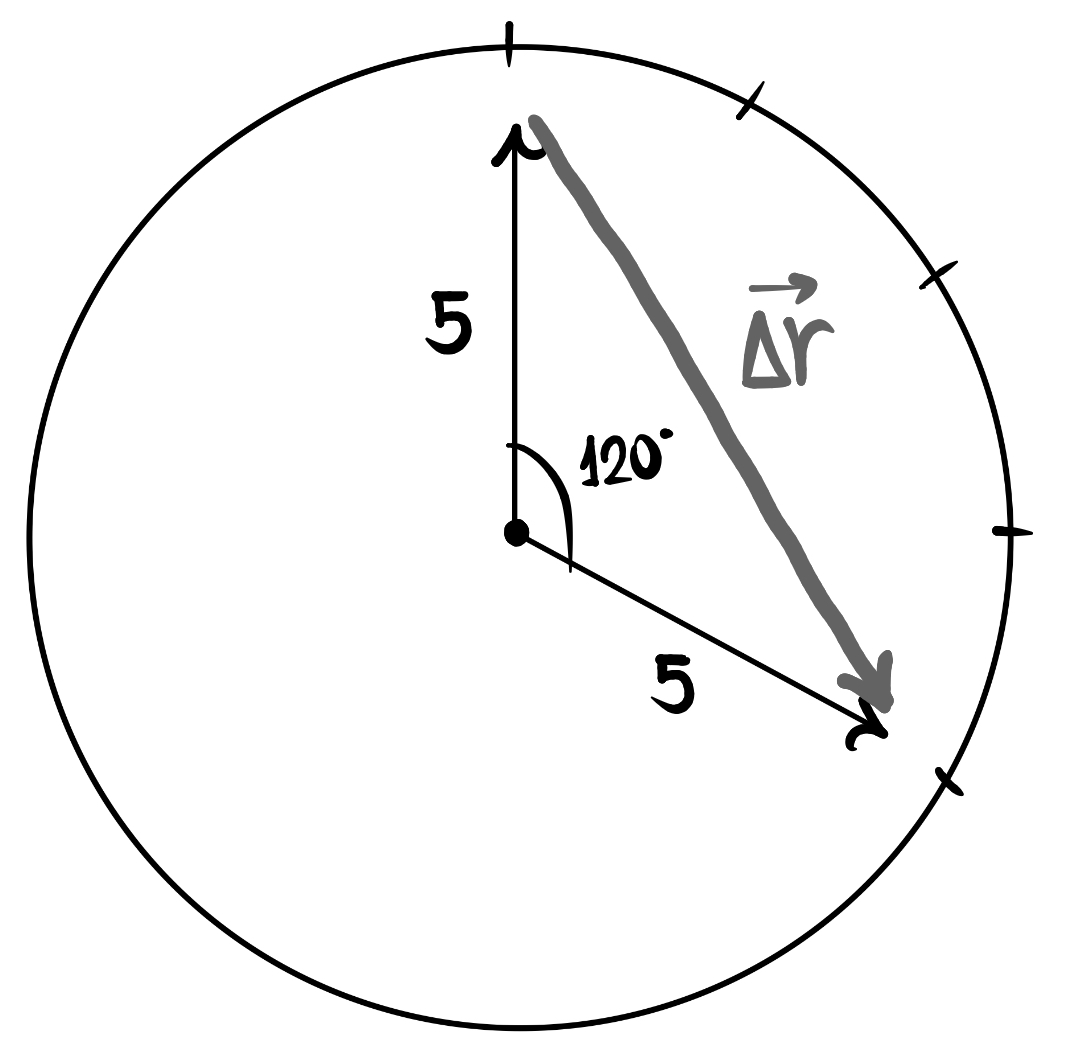
\includegraphics[width=0.3\linewidth]{imagenscinematicavetorial/relogio.jpeg}
\captionof{figure}{}
\label{fig_cinvet_ponteirorelogio}
} 

O vetor deslocamento $\Delta \vec{r}$ vai da posição inicial da extremidade do ponteiro até a sua posição final, e está indicado na mesma imagem. O módulo de tal vetor pode ser computado usando diretamente a Lei dos Cossenos, ou então, por um outro caminho, que consiste em perceber que tal triângulo é isósceles. \\

Assim, sendo seus lados iguais, os ângulos base também o serão, e iguais a $30^\circ$ no caso, para totalizar $180^\circ$ com o ângulo já encontrado de $120^\circ$. Sendo o triângulo isósceles, sua altura será também bissetriz, dividindo o ângulo de $120^\circ$ em dois iguais, e será também mediana, dividindo o módulo do vetor deslocamento em duas partes iguais, como mostra a Figura \ref{fig_cinvet_ponteirorelogio02}.

{
\centering
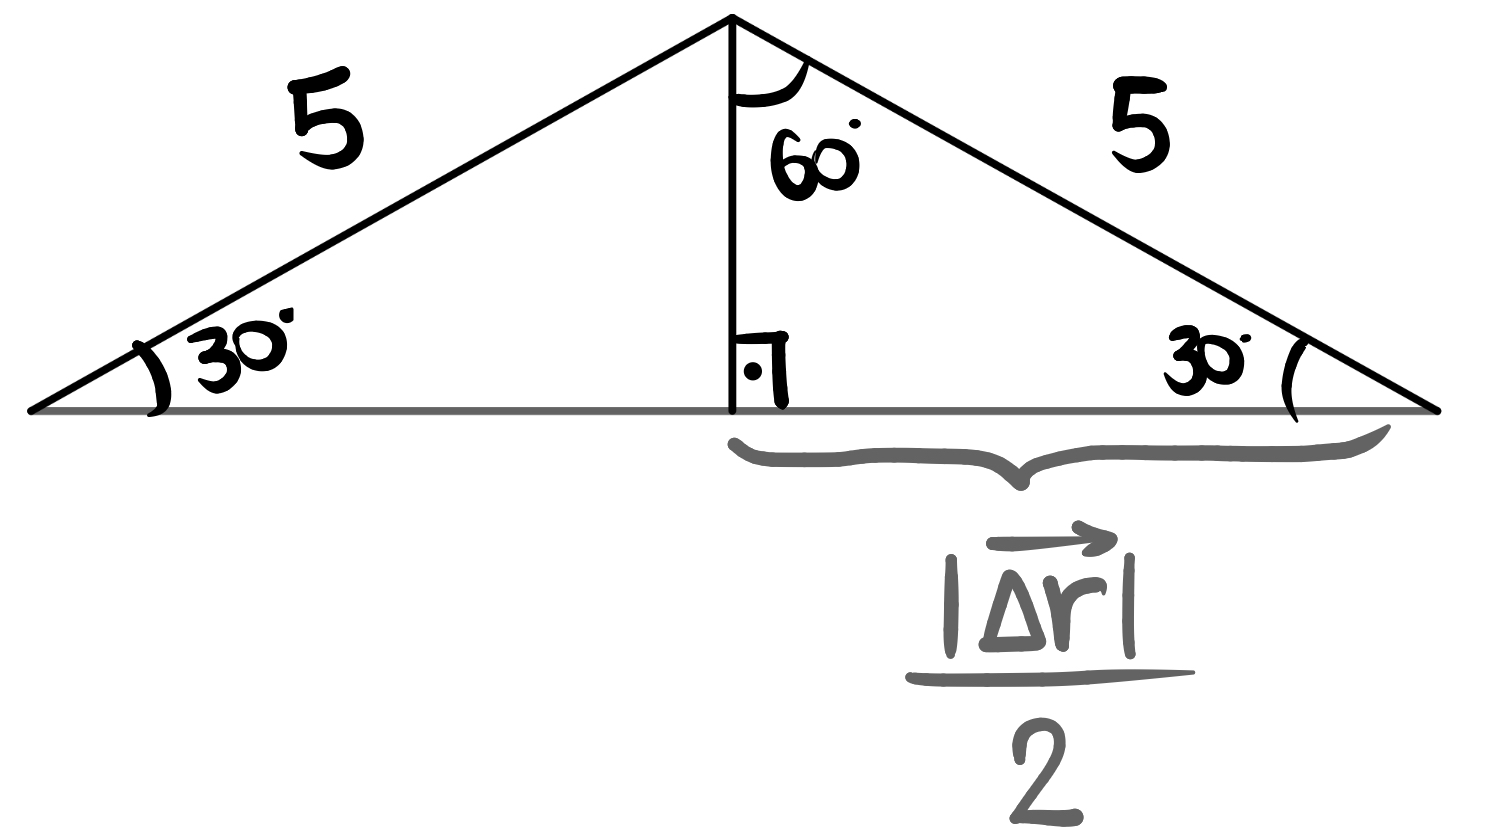
\includegraphics[width=0.3\linewidth]{imagenscinematicavetorial/ponteirorelogio02.jpeg}
\captionof{figure}{}
\label{fig_cinvet_ponteirorelogio02}
} 


Por meio de tal figura o cálculo se dá de forma imediata usando trigonometria básica:

$$ \sin 60^\circ = \dfrac{\sqrt3}{2}=\dfrac{\sfrac{|\Delta \vec{r}|}{2}}{5} \implies |\Delta \vec{r}| = 5\sqrt3 \text{ cm,}$$

\noindent de modo que a velocidade vetorial média é um vetor de módulo

$$ |\vec{v}_m| = \dfrac{|\Delta \vec{r}|}{\Delta t}= \dfrac{5 \sqrt 3 \text{ cm}}{20 \text{ min}} \implies \boxed{|\vec{v}_m| =\dfrac{\sqrt 3}{4} \text{ cm/min.}}$$
    
\end{exemplo}


\vspace{0.3cm}


\begin{exemplo}[Nível III (ITA 2009 - ADAPTADA)]\label{exemplo_cinematicavetorial_velocidadevetorialex03}

Na figura, um ciclista percorre o trecho $AB$ com velocidade escalar média de $22{,}5\ \text{km/h}$ e, em seguida, o trecho $BC$ de $3{,}00\ \text{km}$ de extensão.
No retorno, ao passar em $B$, verifica ser de $20{,}0\ \text{km/h}$ sua velocidade escalar média no percurso então percorrido, $ABCB$.
Finalmente, ele chega em $A$ perfazendo todo o percurso de ida e volta em $1{,}00\ \text{h}$, com velocidade escalar média de $24{,}0\ \text{km/h}$.
Encontre o módulo $v$ do vetor velocidade média referente ao percurso $ABCB$.

\vspace{0.8cm}

\begin{center}
\begin{tikzpicture}[scale=1.05, line cap=round, line join=round]
  % Points
  \coordinate (A) at (0,0);
  \coordinate (B) at (6,0);
  \coordinate (C) at (9,2.2);

  % Path AB (horizontal)
  \draw[thick] (A) -- (B);

  % Path BC (inclined)
  \draw[thick] (B) -- (C);

 

  % Labels
  \node[below] at (A) {$A$};
  \node[below] at (B) {$B$};
  \node[above right] at (C) {$C$};

  % Length label for BC
  \node[rotate=33.5, above] at ($(B)!0.55!(C)$) {$3{,}00\ \text{km}$};
\end{tikzpicture}
\end{center}




\resolucao

Seja $x$ o comprimento do segmento $\overline{AB}$. Como queremos o vetor velocidade média no trecho $ABCB$, vemos que o deslocamento total será o vetor $\overrightarrow{AB},$ uma vez que o ciclista sai de $A$ e termina em $B$. O módulo de tal vetor, sendo $x,$ faz com que o módulo da velocidade vetorial média em todo o trecho seja
$$ |\vec{v}_m| = \dfrac{|\Delta \vec{r}|}{\Delta t},$$

\noindent em que $\Delta t$ é o tempo de movimento do trecho ABCB.\\

Avaliemos a velocidade média no trecho total ABCBA, de 1 hora de duração. Como o enunciado nos diz que a velocidade escalar média em tal trecho é de $24$ km/h, teremos:

$$ v_m = 24 = \dfrac{d}{t} = \dfrac{x+3+3+x}{1} \implies x = 9 \text{ km.}$$

Avaliando o trecho $ABCB,$ sendo de $20,0$ km/h sua velocidade escalar média em tal trecho, temos que sua duração foi de

$$\Delta t = \dfrac{d}{v} = \dfrac{(9+3+3) \text{ km}}{20 \text{ km/h}}= \dfrac{3}{4} \text{ h.}$$

Logo, a velocidade vetorial média no trecho ABCB tem módulo dado por

  $$ |\vec{v}_m| = \dfrac{|\Delta \vec{r}|}{\Delta t} = \dfrac{x}{\Delta t}=\dfrac{9 \text{ km}}{\sfrac{3}{4} \text{ h} } = \boxed{12 \text{ km/h.}}$$
    
\end{exemplo}


\vspace{0.3cm}










\section{Aceleração Vetorial}






\begin{secnivel}[Aceleração Vetorial Média]{I}{Aceleração Vetorial Média}
  
  \eqLdois{def}{cinvet_eq_aceleracaovetorialmedia}{\vec{a}_m  := \dfrac{\Delta \vec{v}}{\Delta t}}

\end{secnivel}




\secgfe{De onde vem}

Essa definição é apenas uma continuação do conceito de aceleração escalar média, em que agora estendemos esse conceito para absorver o caráter vetorial da velocidade.

Assim, tendo definido a velocidade vetorial, fica natural definir a aceleração vetorial média como sendo a variação de tal grandeza no tempo, ou seja:

$$ \vec{a}_m = \dfrac{\Delta \vec{v}}{\Delta t} = \dfrac{\vec{v}-\vec{v_0}}{t-t_0},$$

\noindent em que $\vec{v}$ é a velocidade do objeto no instante $t,$ e $\vec{v}_0$ é a velocidade do objeto no instante $t_0.$

Como já investimos muito tempo em discutir qual é o sentido em se definir a aceleração média como o fizemos -- na parte sobre Cinemática Escalar -- parece razoável ser mais sucinto nesse momento. A lógica agora é realmente apenas ampliar tal conceito para incorporar o caráter vetorial da velocidade.


\secgfe{Onde é usada}

Tal como comentamos acerca de Equação \eqref{cinvet_eq_velocidadevetorialmedia}, algo semelhante se aplica à Equação \eqref{cinvet_eq_aceleracaovetorialmedia}: ela é, de forma direta, bem pouco usada. Será raro o leitor se deparar com algum contexto físico, problema ou exercício em que ele precise usar diretamente tal equação.

Ela, contudo, é usada como passo intermediário para construir outras equações que usaremos mais, como, por exemplo, a da aceleração centrípeta. Sendo assim, a importância da Equação \eqref{cinvet_eq_aceleracaovetorialmedia} se dará mais pelo que decorrerá dela do que do uso direto em si.


\secgfe{Erros comuns}

Os erros mais comuns aqui costumam ser de geometria ou trigonometria. Como a equação em questão é vetorial, o cálculo de $\Delta \vec{v}$ envolve a subtração de dois vetores -- a velocidade final e inicial. Logo, a geometria de tal cálculo irá depender da direção desses vetores, e o seu cálculo poderá envolver alguns teoremas da geometria plana como o Teorema de Pitágoras, a Lei dos Senos e Cossenos, ou noções básicas de trigonometria como aplicação de seno, cosseno e tangente em triângulos retângulos.

O leitor que não estiver muito afiado nesses conceitos possivelmente encontrará dificuldades em fazer cálculos envolvendo a Equação \eqref{cinvet_eq_aceleracaovetorialmedia}



\secgfe{Observações}

Como pontuamos, o que estamos fazendo aqui é apenas uma extensão do conceito escalar de aceleração. Assim, é interessante notar que essa nova definição de aceleração média incorpora, como casos particulares, o que já conhecíamos como aceleração. 

Note, por exemplo, o movimento da Figura \ref{fig_cinvet_aceleracaovetorialecasoparticular1}, que mostra um MU em linha reta. Como sabemos, em tal movimento a aceleração é nula, o que de fato ocorre caso façamos o cálculo por meio da Equação \eqref{cinvet_eq_aceleracaovetorialmedia}, como é mostrado no lado direito da figura. Ali, tomamos o instante final $t=2$s e sua velocidade ali, cujo módulo é $|\vec{v}_f|=2$ m/s, apontando para a direita. Já a velocidade inicial $\vec{v}_0$ é aquela em $t=0$s, cujo módulo é $|\vec{v}_0|=2$ m/s e também aponta para direita. 

Assim, fazendo a variação $\Delta \vec{v} = \vec{v_f}-\vec{v}_0,$ chegamos, naturalmente, em um vetor nulo, de modo que a aceleração vetorial média será $\sfrac{\Delta \vec{v}}{\Delta t}= \vec 0,$ como esperado\footnote{Usamos aqui o zero como vetor para manter a coerência: do lado esquerdo da equação temos um vetor, calculado por $\sfrac{\Delta \vec{v}}{\Delta t}$, de modo que o lado direito também deve ser o vetor. O vetor $\vec 0$ é o vetor nulo: seu módulo é zero, de modo que sua direção e sentido são irrelevantes haja vista que ele não aponta para lugar algum.}. Caso o leitor avalie em quaisquer outros intervalos de tempo chegará sempre no mesmo resultado, e a conclusão -- que já sabíamos, mas sem usar o caráter vetorial até então -- é de que a aceleração é nula ao longo do Movimento Uniforme.

\vspace{0.3cm}

{
\centering
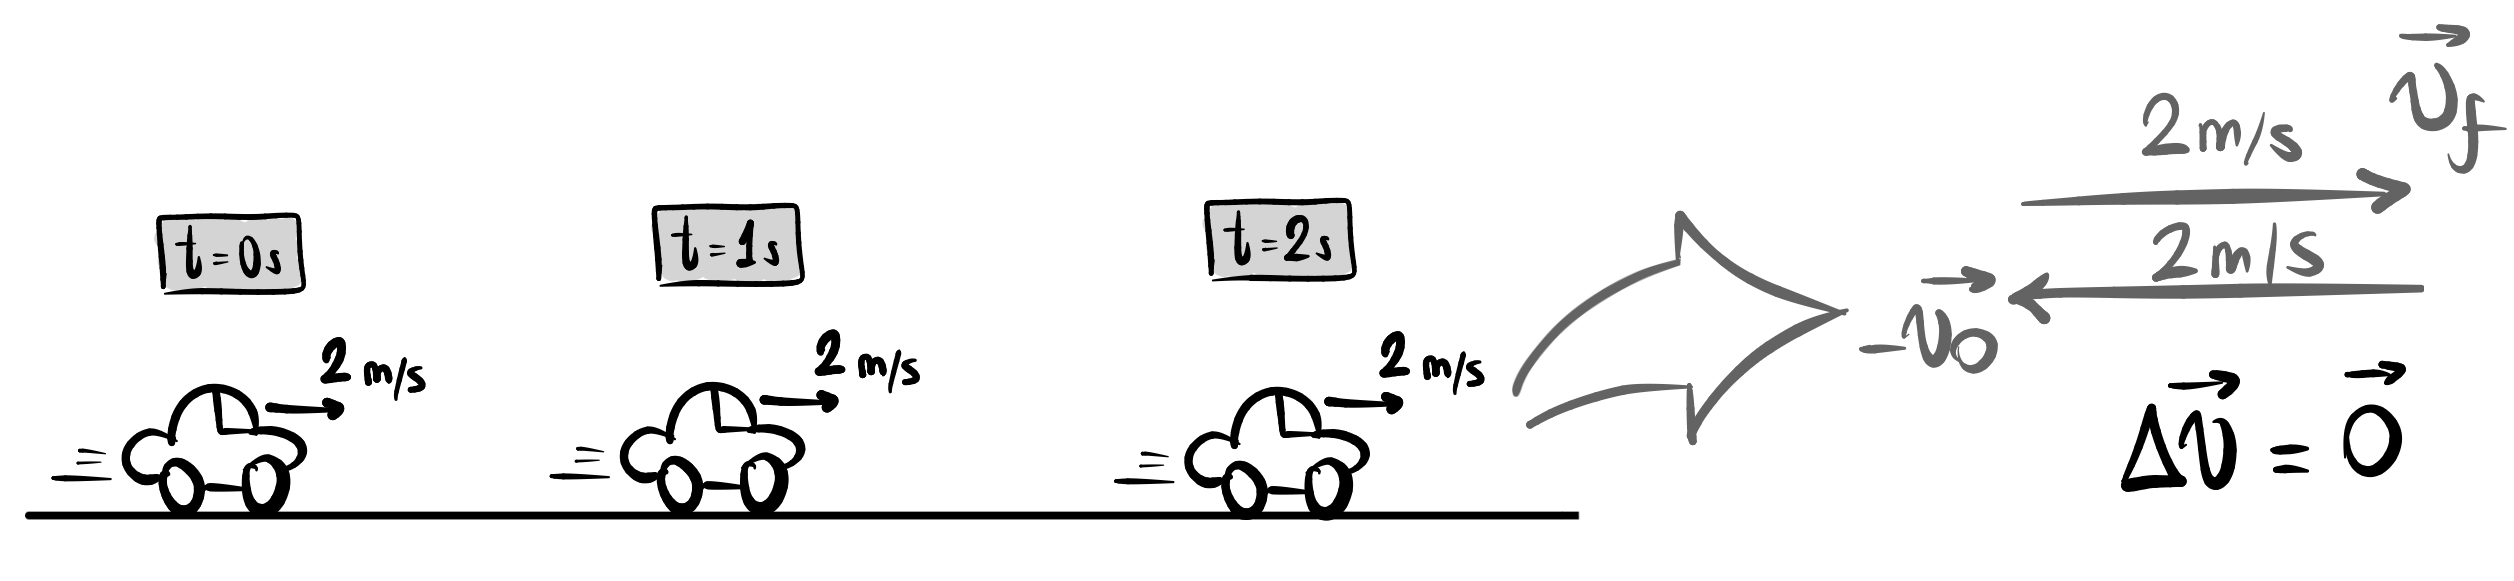
\includegraphics[width=0.85\linewidth]{imagenscinematicavetorial/aceleracaovetorialecasoparticular1.jpeg}
\captionof{figure}{O conceito de aceleração vetorial média aplicada ao Movimento Uniforme em linha reta.}
\label{fig_cinvet_aceleracaovetorialecasoparticular1}
} 

\vspace{0.3cm}

Um outro caso particular pode ser observado na Figura \ref{fig_cinvet_aceleracaovetorialecasoparticular2}, que mostra um Movimento Uniformemente Variado em linha reta. Novamente, tomamos o instante final $t=2$s e sua velocidade ali, cujo módulo é $|\vec{v}_f|=1$ m/s, apontando para a direita. Já a velocidade inicial $\vec{v}_0$ é aquela em $t=0$s, cujo módulo é $|\vec{v}_0|=7$ m/s e também aponta para direita. 

\vspace{0.3cm}

{
\centering
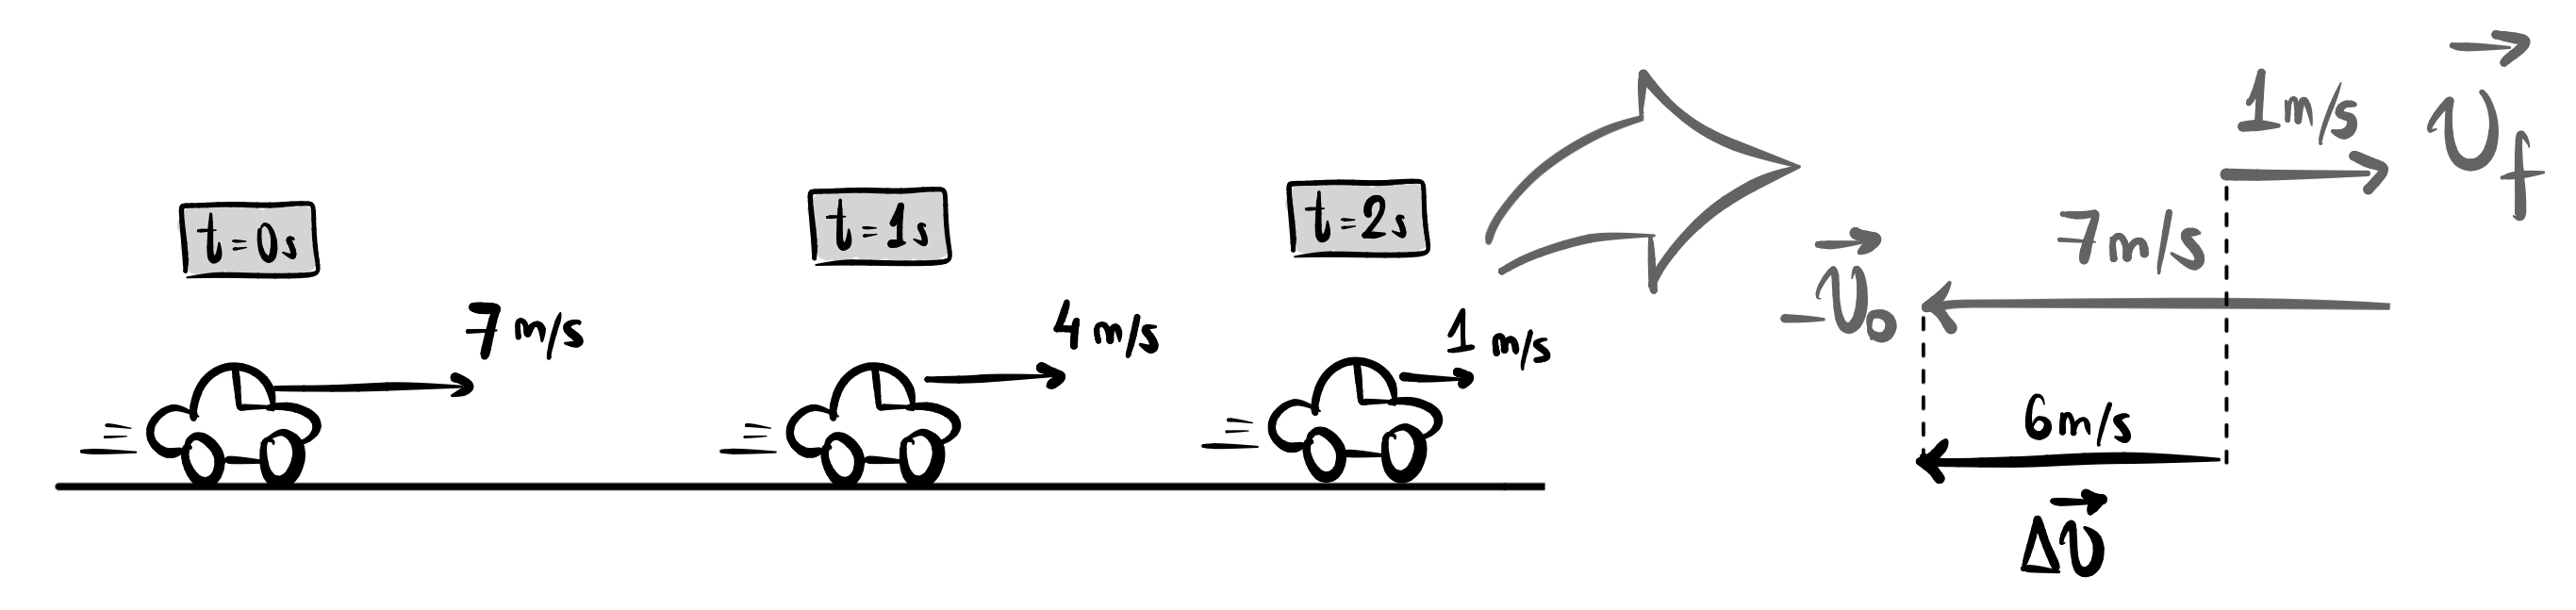
\includegraphics[width=0.8\linewidth]{imagenscinematicavetorial/aceleracaovetorialecasoparticular2.jpeg}
\captionof{figure}{O conceito de aceleração vetorial média aplicada ao Movimento Uniformemente Variado em linha reta.}
\label{fig_cinvet_aceleracaovetorialecasoparticular2}
} 

\vspace{0.3cm}

O lado direito da imagem mostra o esboço do cálculo da variação $\Delta \vec{v} = \vec{v_f}-\vec{v}_0,$ que resulta em um vetor de tamanho $6$, isto é, $|\Delta \vec{v}|=6$ m/s, porém apontando para a esquerda. Assim, a aceleração vetorial média nos dois segundos de movimento tem módulo igual a

$$ |\vec{a}_m| = \dfrac{|\Delta \vec{v}|}{\Delta t} = \dfrac{6 \text{ m/s}}{2 \text{ s}} \implies \boxed{ |\vec{a}_m|=3 \text{ m/s$^2$},}$$

\noindent apontando para a esquerda -- que é o sentido do vetor $\Delta \vec{v}$ --, de modo que o movimento é retardado. Calculando a aceleração entre quaisquer dois instantes de tempo -- e usando a definição escalar de aceleração -- o leitor será levado ao mesmo resultado.

Com isso, fica claro que nossa nova definição de aceleração média incorpora todo o conceito de aceleração que já conhecíamos, e, na verdade, estende-o para um campo de aplicação ainda maior, uma vez que, com o caráter vetorial embutido na definição, poderemos tratar de movimentos bidimensionais, o que antes não era possível.

\vspace{0.3cm}
%Exemplo resolvido

\begin{exemplo}[Nível I]\label{exemplo_cinematicavetorial_aceleracaovetorialexemplo01}

Considere a situação ilustrada na Figura \ref{fig_cinvet_aceleracaovetorialmediaex01}. Calcule, entre os instantes $t=0$s e $t=2$s, a aceleração escalar média do corpo e a sua aceleração vetorial média.

{
\centering
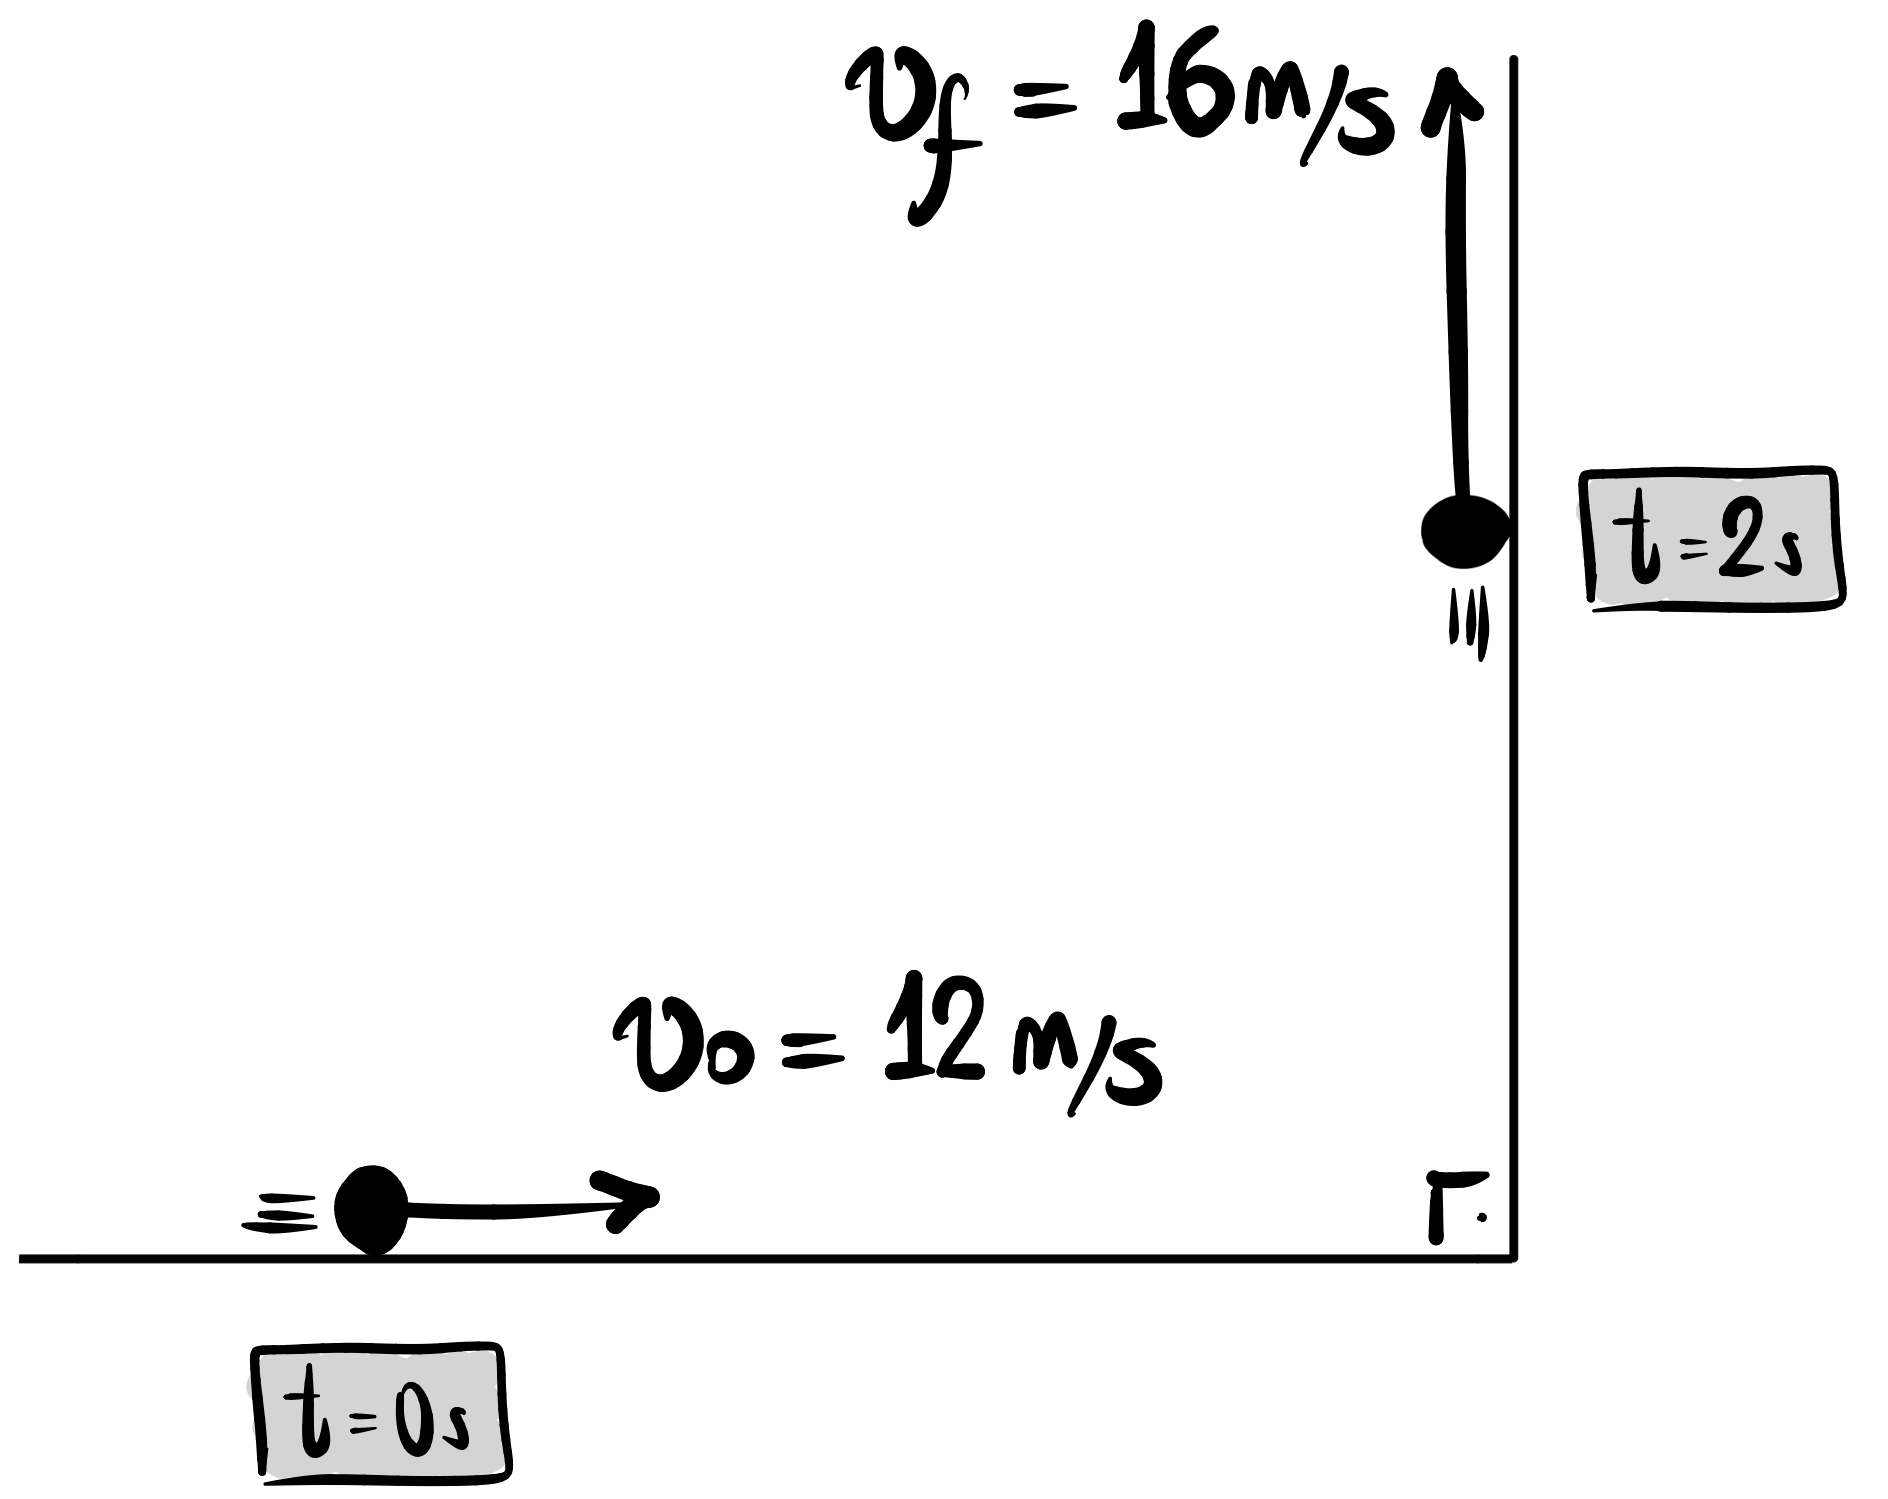
\includegraphics[width=0.35\linewidth]{imagenscinematicavetorial/aceleracaovetorialmediaex01.jpeg}
\captionof{figure}{}
\label{fig_cinvet_aceleracaovetorialmediaex01}
} 

\resolucao


Este é UM ótimo exemplo para percebermos a diferença entre a aceleração vetorial e a aceleração escalar. Faremos aqui, portanto, uma extensa digressão a fim de tornar clara essa diferença e suas nuances. Vamos por partes:

\begin{enumerate}
    \item [(a)] Aceleração Escalar Média

    Essa grandeza mede apenas o quanto varia o valor, isto é, o módulo, da velocidade. Sendo assim, seu cálculo é imediato:

    $$ a_m=\dfrac{\Delta v}{\Delta t}=\dfrac{16-12}{2-0} \implies \boxed{a_m=2 \text{ m/s$^2$.}}$$


     \item [(b)] Aceleração Vetorial Média

     Agora o que importa não são apenas os valores, isto é, os módulos das velocidades, mas também sua direção e sentido, já que elas influenciarão na geometria do problema. Observe a Figura \ref{fig_cinvet_aceleracaovetorialmediaex012}, que esboça o cálculo de $\Delta \vec{v}=\vec{v}_f-\vec{v}_0.$

{
\centering
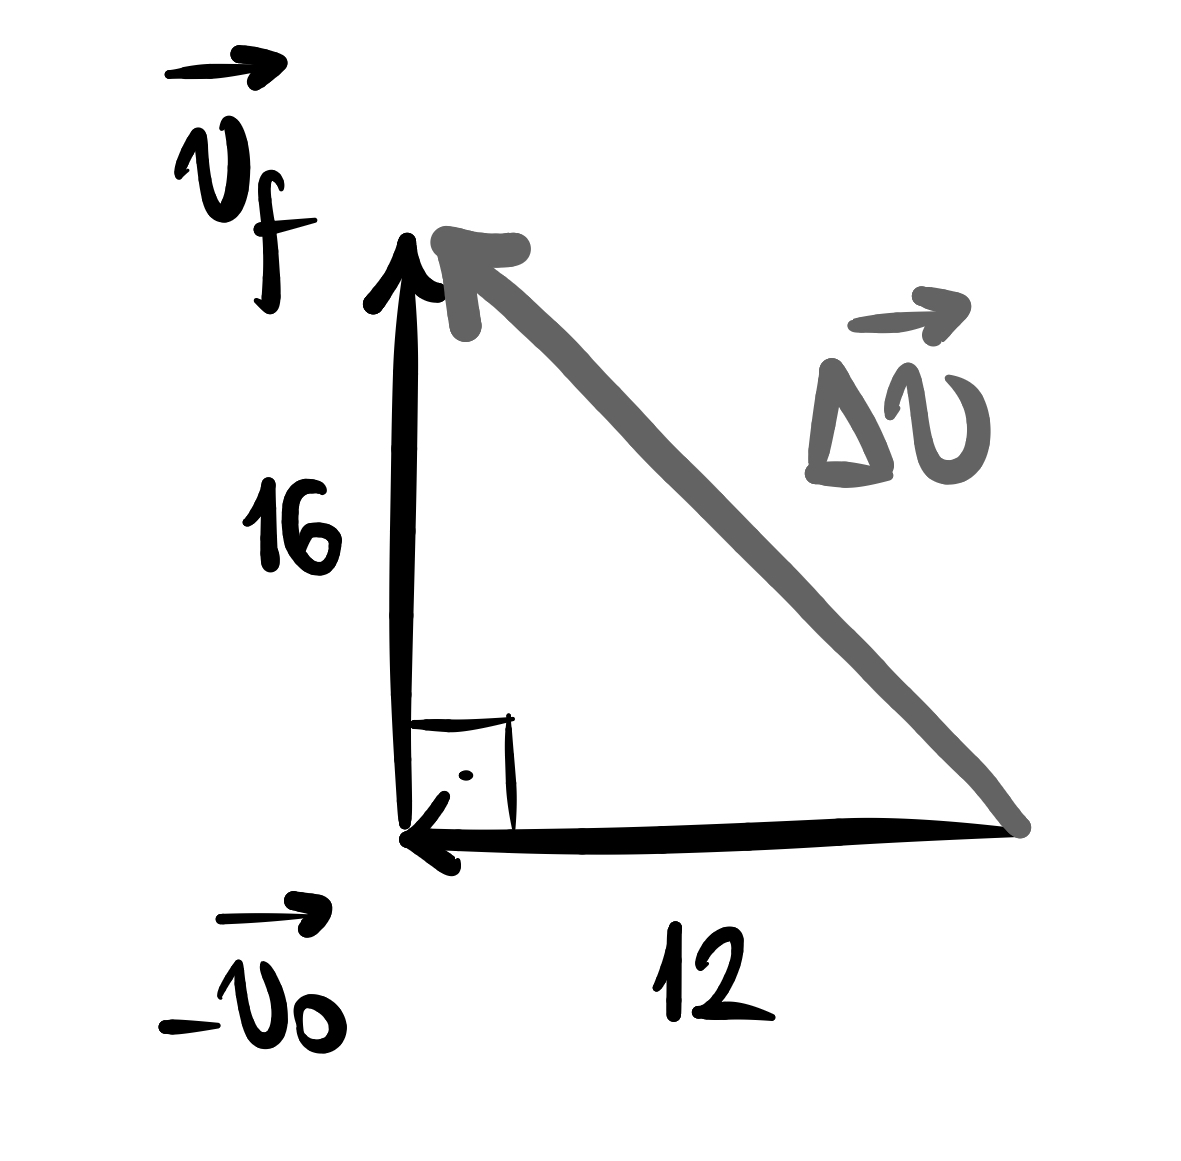
\includegraphics[width=0.25\linewidth]{imagenscinematicavetorial/aceleracaovetorialmediaex012.jpeg}
\captionof{figure}{}
\label{fig_cinvet_aceleracaovetorialmediaex012}
} 

A partir de tal figura é imediato calcular o módulo da variação da velocidade, que é obtido pelo Teorema de Pitágoras:

$$ |\Delta \vec{v}|^2 = 12^2+16^2 \implies |\Delta \vec{v}| = 20 \text{ m/s},$$

\noindent de modo que o módulo da aceleração vetorial média é

$$ |\vec{a}_m| = \dfrac{|\Delta \vec{v}|}{\Delta t} = \dfrac{20 \text{ m/s}}{2 \text{ s}} \implies \boxed{|\vec{a}_m|=10 \text{ m/s$^2$}.}$$

     
\end{enumerate}

Pois bem...as respostas não coincidiram. Em um primeiro momento isso pode parecer estranho, mas, na verdade era algo a se esperar. Cabe destacarmos algumas observações importantes sobre este fato:


\begin{enumerate}
    \item [(i)] Coincidência entre os cálculos escalar e vetorial.

    Os valores da aceleração escalar e do módulo da aceleração vetorial só vão coincidir em movimentos unidimensionais, como já exposto. Na seção sobre \textbf{observações} a respeito da Equação \eqref{cinvet_eq_velocidadevetorialmedia} deixamos isso claro com os exemplos do MU e do MUV em linha reta. 
    
    A questão, no contexto deste exemplo, é que o movimento muda de direção -- e a aceleração escalar não consegue capturar essa informação. Observe que, do ponto de vista da aceleração escalar, as velocidades da Figura \ref{fig_cinvet_axeaxyaceleracaovetorial1} são iguais -- duas velocidades cujo valor é de $10$ m/s. 

{
\centering
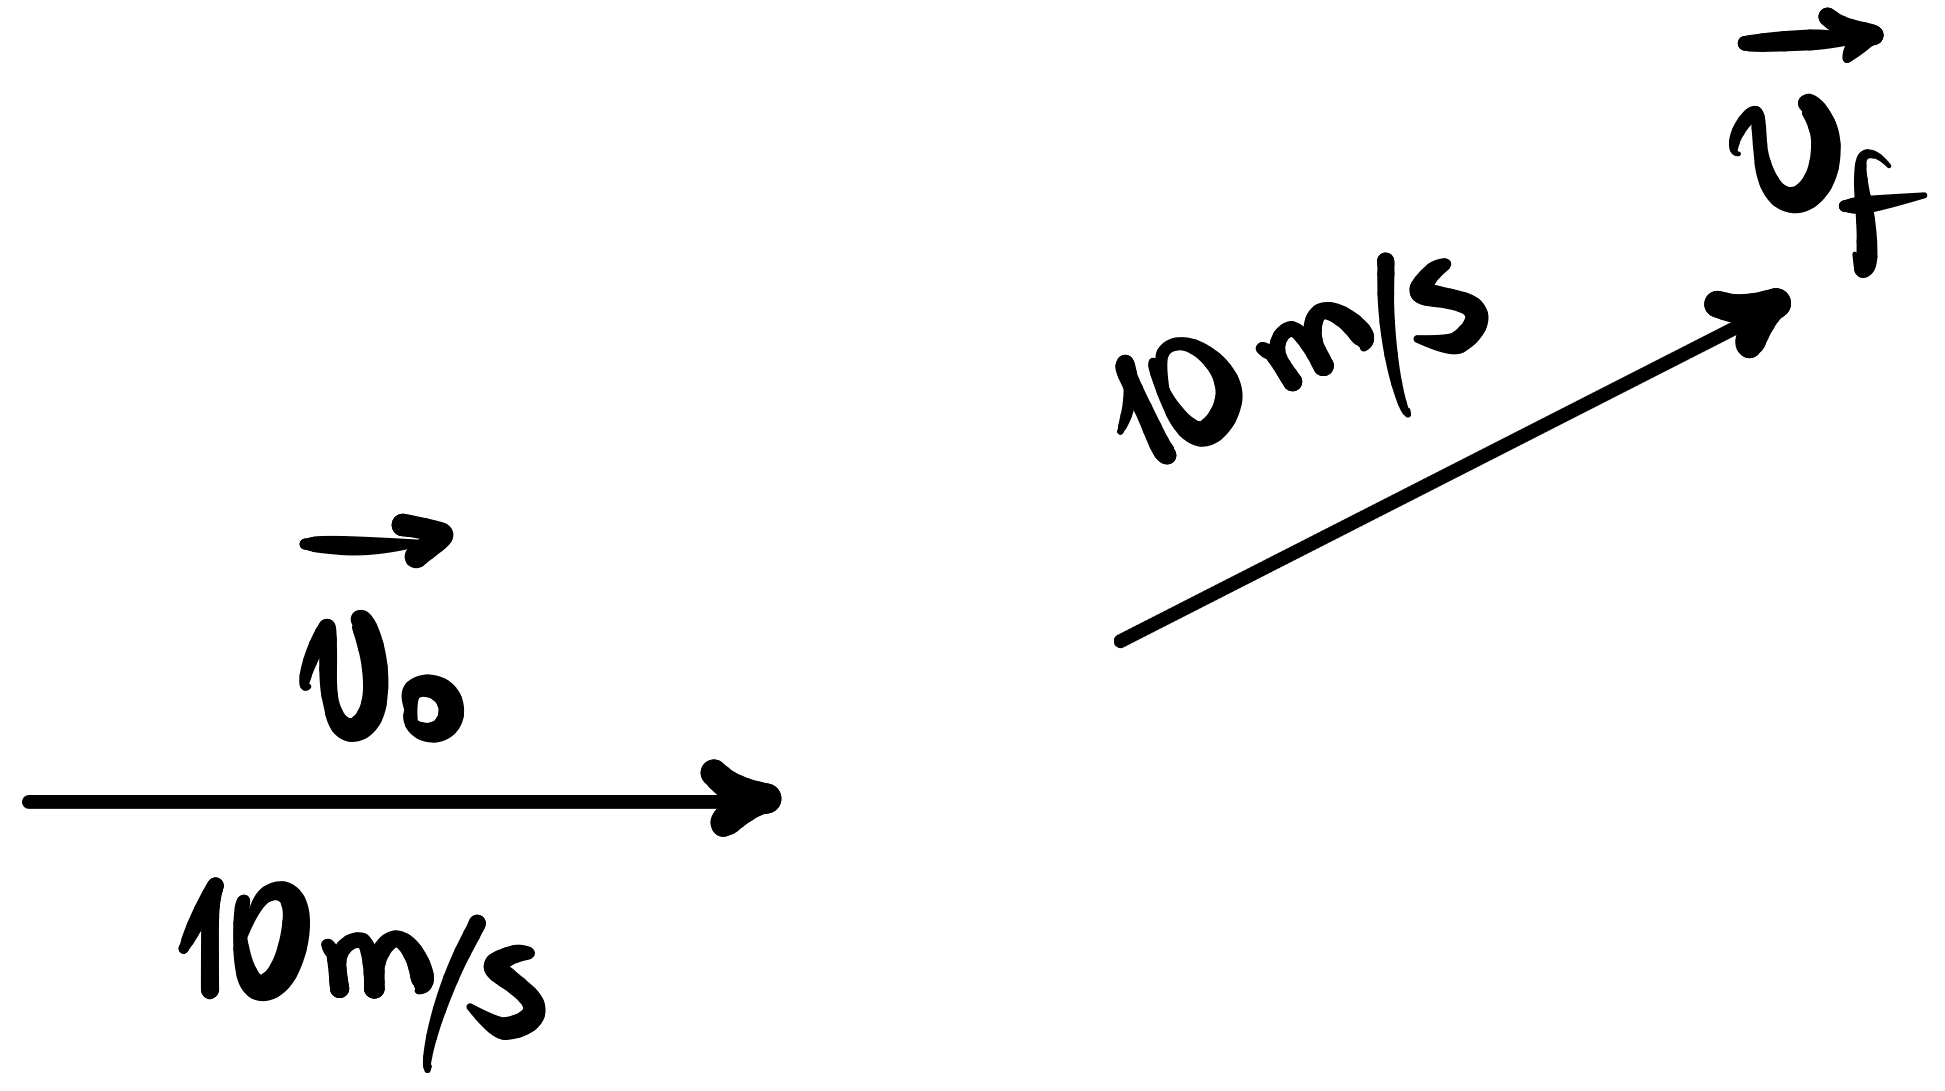
\includegraphics[width=0.30\linewidth]{imagenscinematicavetorial/axeaxyaceleracaovetorial1.jpeg}
\captionof{figure}{}
\label{fig_cinvet_axeaxyaceleracaovetorial1}
} 
    
    
    \item [(ii)] Caráter vetorial da velocidade.

    O fato de termos obtido valores distintos para as acelerações neste exemplo é por que, enquanto a aceleração escalar só percebe a variação do valor da velocidade, que foi de $16-12=4$ m/s, a aceleração vetorial captura também a variação vetorial da velocidade, isto é, a variação da sua direção. Voltemos, por exemplo, ao caso da Figura \ref{fig_cinvet_axeaxyaceleracaovetorial1}. Digamos que a velocidade $\vec{v}_f$ faça um ângulo $\theta$ com a horizontal -- direção da velocidade $\vec{v}_0$ -- tal que  $\sin \theta = 0.6 \quad \text{ e } \quad \cos \theta = 0.8.$ 
    
    Neste caso, obtemos, por trigonometria básica, que

    $$ \sin \theta = \dfrac{v_y}{10}=0.6 \implies \boxed{v_y= 6 \text{ m/s}} \quad \text{ e } \quad \cos \theta = \dfrac{v_x}{10}=0.8 \implies \boxed{v_x= 8 \text{ m/s},}$$
    
\noindent como mostra a Figura \ref{fig_cinvet_axeaxyaceleracaovetorial2}.

{
\centering
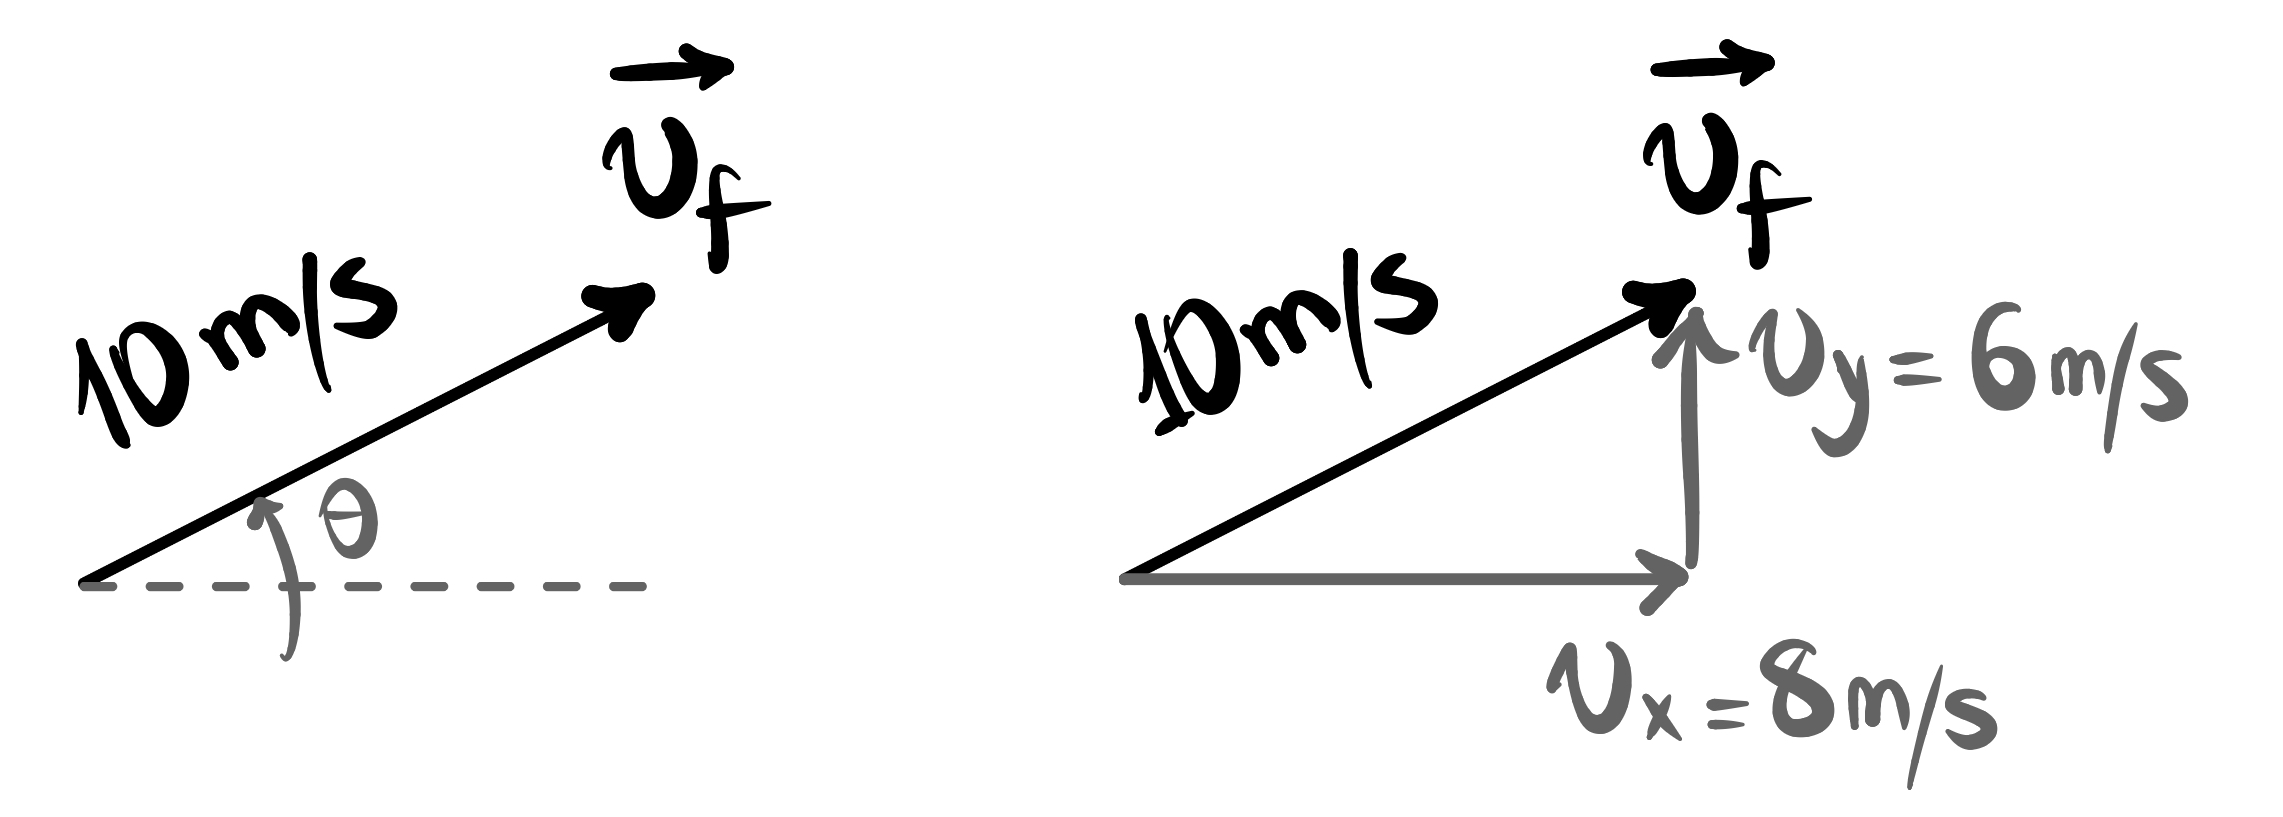
\includegraphics[width=0.50\linewidth]{imagenscinematicavetorial/axeaxyaceleracaovetorial2.jpeg}
\captionof{figure}{}
\label{fig_cinvet_axeaxyaceleracaovetorial2}
} 

Assim, a velocidade $\vec{v}_f$ pode ser interpretada como composta por uma velocidade horizontal $\vec{v}_x$ cujo módulo é de $8$ m/s, e uma velocidade vertical $\vec{v}_y$ cujo módulo é de $6$ m/s. Neste caso, comparar as velocidades $\vec{v}_0$ e $\vec{v}_f$ da Figura \ref{fig_cinvet_axeaxyaceleracaovetorial1} deixa evidente como elas são diferentes, como destaca a Figura \ref{fig_cinvet_axeaxyaceleracaovetorial3}.



{
\centering
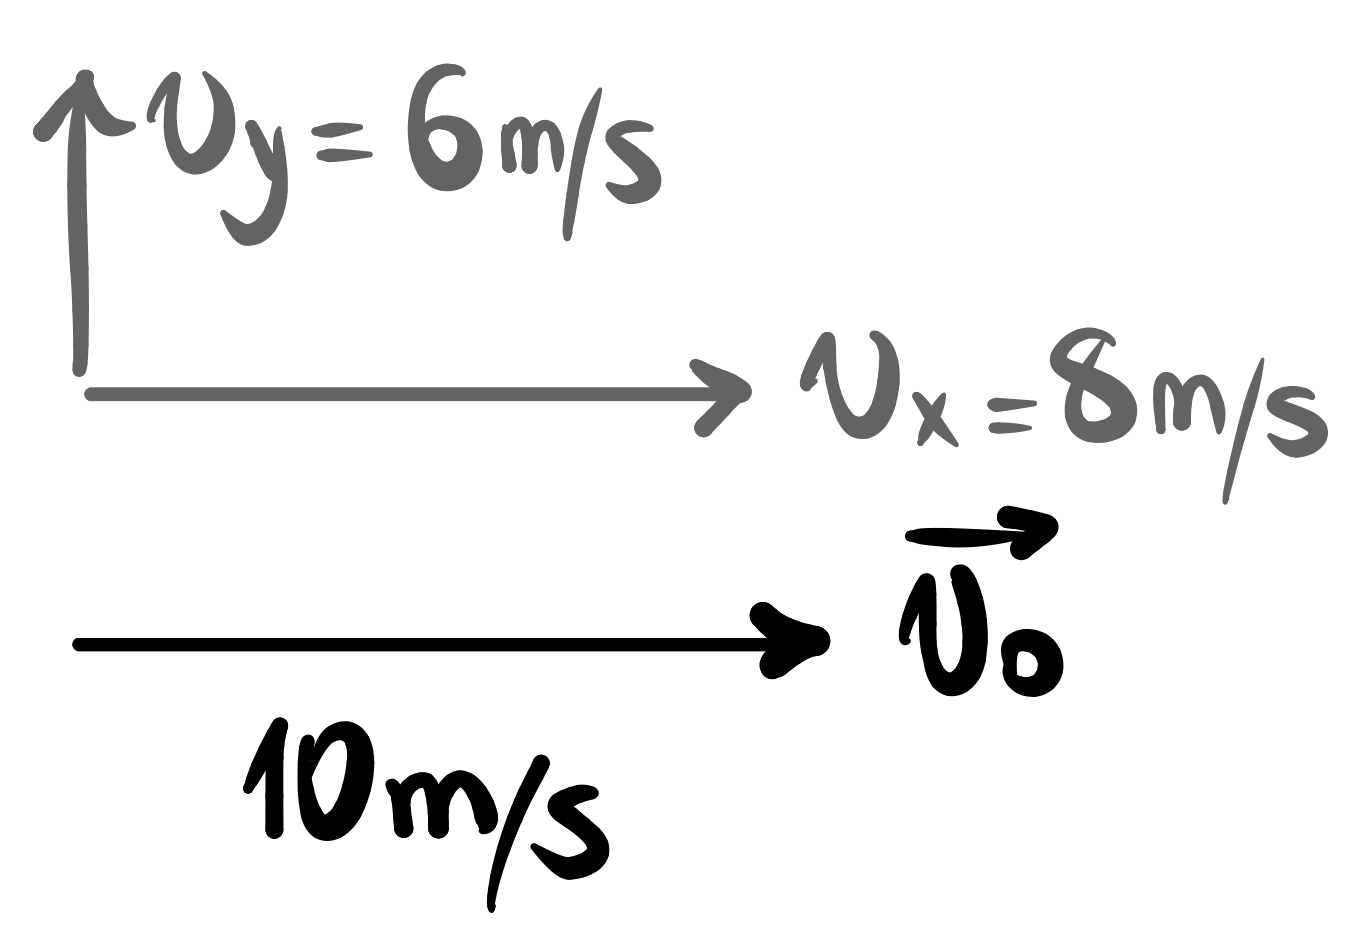
\includegraphics[width=0.30\linewidth]{imagenscinematicavetorial/axeaxyaceleracaovetorial3.jpeg}
\captionof{figure}{}
\label{fig_cinvet_axeaxyaceleracaovetorial3}
} 

Para alterar a velocidade do seu estado inicial $\vec{v_0}$ e fazer com que se chegue no estado final $\vec{v}_f$ \textbf{é preciso alterar seu valor em duas dimensões}: diminuir em $2$ m/s a componente horizontal e aumentar em $6$ m/s a componente vertical. 

E é por isso que a aceleração escalar fornece um resultado diferente: ela ignora o caráter bidimensional do movimento por olhar apenas para o valor absoluto da velocidade, e não para o que acontece com a velocidade enquanto ente geométrico.

    \item [(iii)] Análise por componentes.

Uma perspectiva final que vale pontuar é que a aceleração vetorial pode ser interpretada, no contexto deste problema, como uma espécie de aceleração escalar composta em duas dimensões. 

Voltando ao problema do exemplo e avaliando o movimento separadamente nas suas componentes horizontal e vertical, como fizemos no final do tópico acima, podemos entender que, para sair do estado inicial e chegar no estado final, é preciso desacelerar completamente na horizontal, indo de $v_{0}=12$ m/s até $0$ m/s, o que exigiria uma variação de velocidade horizontal de

$$ \Delta v_x  =0-12 = -12\text{ m/s},$$

\noindent o que significa, no intervalo de tempo de $2$s, haver uma aceleração horizontal $a_x$ que retarda a partícula dada por

$$a_x=\dfrac{\Delta v_x}{\Delta t} = \dfrac{-12 \text{ m/s}}{2\text{ s}} = -6 \text{ m/s$^2$},$$

\noindent em que o sinal negativo só indica que aceleração possui sentido contrário ao da velocidade inicial, ou seja, o movimento de fato é retardado.

{
\centering
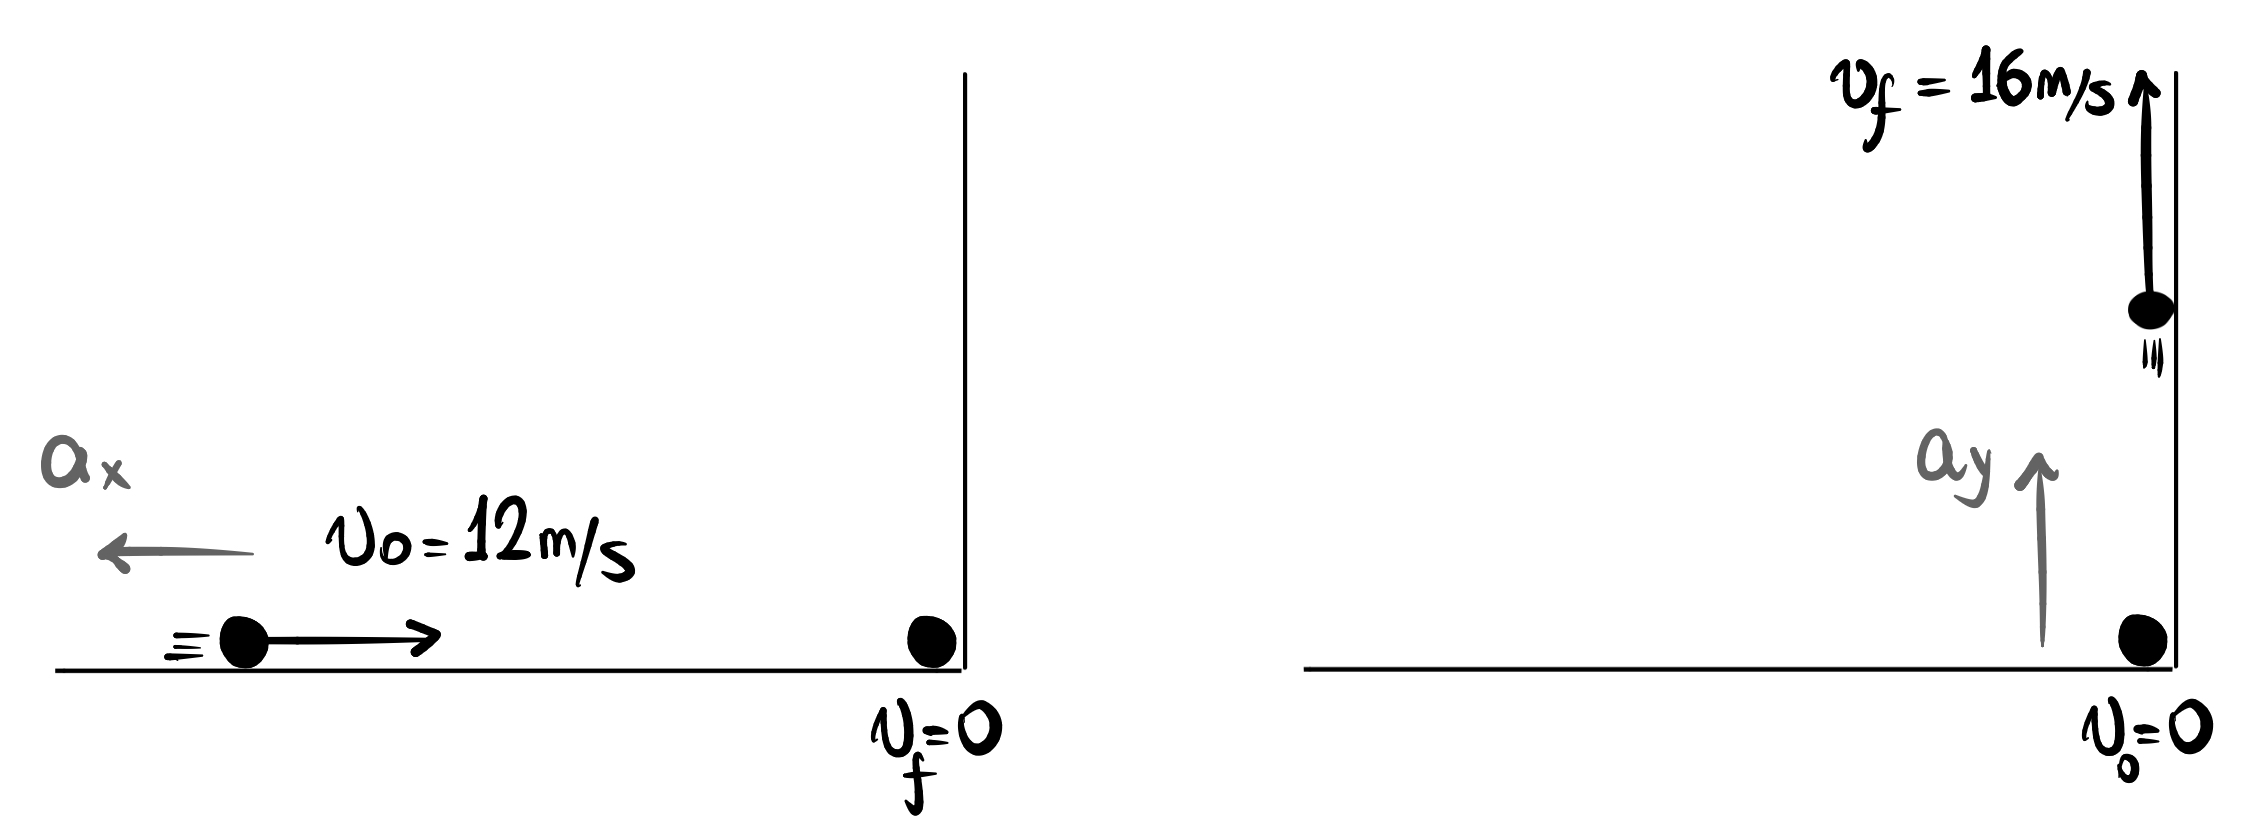
\includegraphics[width=0.80\linewidth]{imagenscinematicavetorial/axeaxyaceleracaovetorial4.jpeg}
\captionof{figure}{}
\label{fig_cinvet_axeaxyaceleracaovetorial4}
} 


Após ter desacelerado totalmente na horizontal, é preciso agora que a nossa partícula, saindo do repouso, adquira uma velocidade de $16$ m/s na direção vertical, a fim de alcançar o estado final de movimento do contexto. Assim, haverá uma variação de velocidade vertical dada por

$$\Delta v_y  = 16-0 = 16\text{ m/s}, $$

\noindent o que significa, no intervalo de tempo de $2$s, haver uma aceleração vertical $a_y$ que acelere a partícula dada por

$$a_y=\dfrac{\Delta v_y}{\Delta t} = \dfrac{16 \text{ m/s}}{2\text{ s}} = 8 \text{ m/s$^2$}.$$

Tal situação aparece ilustrada na Figura \ref{fig_cinvet_axeaxyaceleracaovetorial4}, em que imaginamos o movimento completo como sendo uma desaceleração horizontal $a_x$ que leva a partícula até o repouso logo antes de encostar na parede e, na sequência, uma aceleração vertical $a_y$ que tira a partícula do repouso e a leva à velocidade vertical de $16$ m/s. 

Quebramos o movimento nesses dois estágios para fins didáticos, mas as duas coisas acontecem ao mesmo tempo -- enquanto a partícula desacelera na horizontal ela acelera na vertical -- de modo que o tempo no qual as ``duas acelerações'' atuam é o mesmo, o tempo total de $2$ segundos do movimento completo.


{
\centering
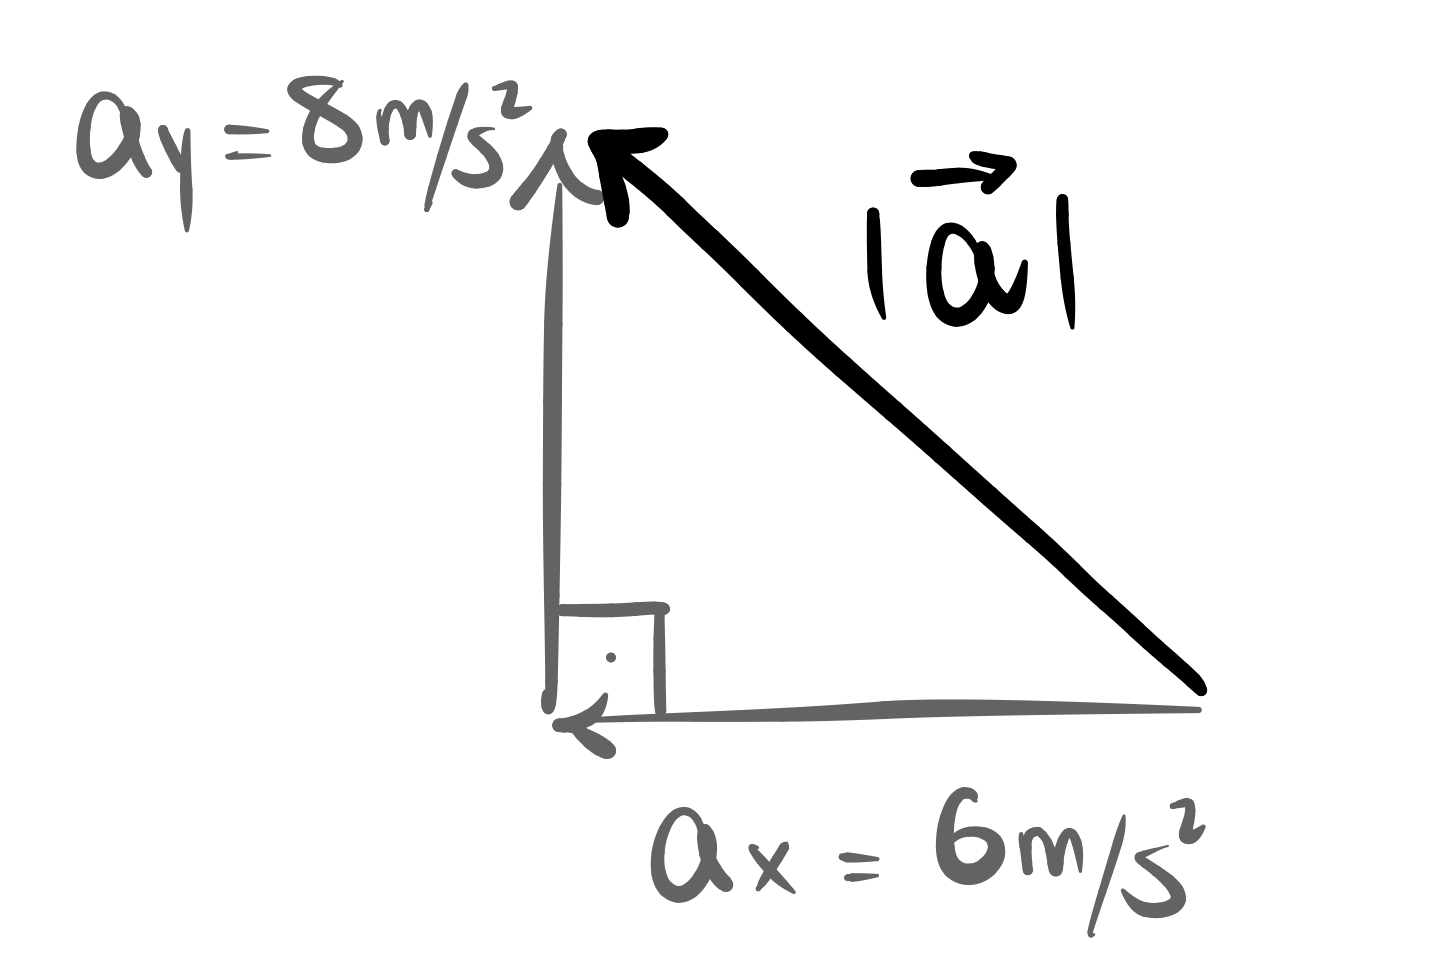
\includegraphics[width=0.30\linewidth]{imagenscinematicavetorial/fig_cinvet_axeaxyaceleracaovetorial5.jpeg}
\captionof{figure}{}
\label{fig_cinvet_axeaxyaceleracaovetorial5}
} 

Sendo assim, encontraríamos que a aceleração total do objeto seria o efeito resultante das acelerações $a_x$ e $a_y$, dado, pelo Teorema de Pitágoras no triângulo da Figura \ref{fig_cinvet_axeaxyaceleracaovetorial5}:

$$ |\vec{a}_m|^2 = a_x^2+a_y^2 = 6^2+8^2 \implies \boxed{|\vec{a}_m|=10 \text{ m/s$^2$}.}$$

Note que este foi o mesmo resultado obtido no cálculo do item $(b)$ do exemplo, porém agora usando, em cada dimensão, o conceito de aceleração escalar. Convida-se, neste momento, o leitor a comparar a Figura \ref{fig_cinvet_aceleracaovetorialmediaex012} com a figura acima, de modo a concluir que, em certa medida, a aceleração vetorial é uma superposição -- em duas dimensões -- do conceito de aceleração escalar, o qual só se aplicava para uma dimensão.
    
\end{enumerate}

    
\end{exemplo}


\vspace{0.3cm}


\begin{exemplo}[Nível II]\label{exemplo_cinvet_acelvetorialnivel2}

Considere um objeto que se move com uma velocidade de valor constante e igual a $10$m/s ao longo de uma trajetória circular. Se o objeto leva $12$ segundos para completar uma volta, calcule o módulo da sua aceleração vetorial média entre 

\begin{enumerate}
    \item [(a)] $t_1=3$s e $t_2=15$s.
    \item [(b)] $t_1=3$s e $t_2=9$s.
    \item [(c)] $t_1=3$s e $t_2=6$s.
    \item [(d)] $t_1=3$s e $t_2=5$s.
\end{enumerate}


\resolucao


Vale destacar que, como o objeto possui velocidade de módulo constante, a aceleração escalar seria zero qualquer que fosse o intervalo de tempo considerado. Assim, o que computarmos aqui como módulo da aceleração vetorial será relativo à aceleração responsável por variar a direção do vetor velocidade, e não o seu módulo, uma vez que este é constante em todo o movimento.

Vamos avaliar cada item separadamente:

\begin{enumerate}
    \item [(a)]  Perceba que os valores específicos dos instantes de tempo são pouco relevantes, o que importa é o intervalo de tempo. Para o primeiro caso, por exemplo, temos $\Delta t = t_2-t_1=15-3=12$s, ou seja, a partícula terá completado uma volta completa.

    Logo, as posições inicial e final sendo as mesmas, os vetores velocidade inicial também o serão, de modo que a sua variação será nula, e, sendo $|\Delta \vec{v}|=0,$ a aceleração vetorial média será nula neste intervalo de tempo.

    \item [(b)] Neste caso o intervalo de tempo é $\Delta t = t_2-t_1=9-3=6$s, de modo que a partícula terá completado meia volta, situação ilustrada na Figura \ref{fig_cinvet_aceleracaovetorialmediaexemplo0101}. 
    
    
    
    {
\centering
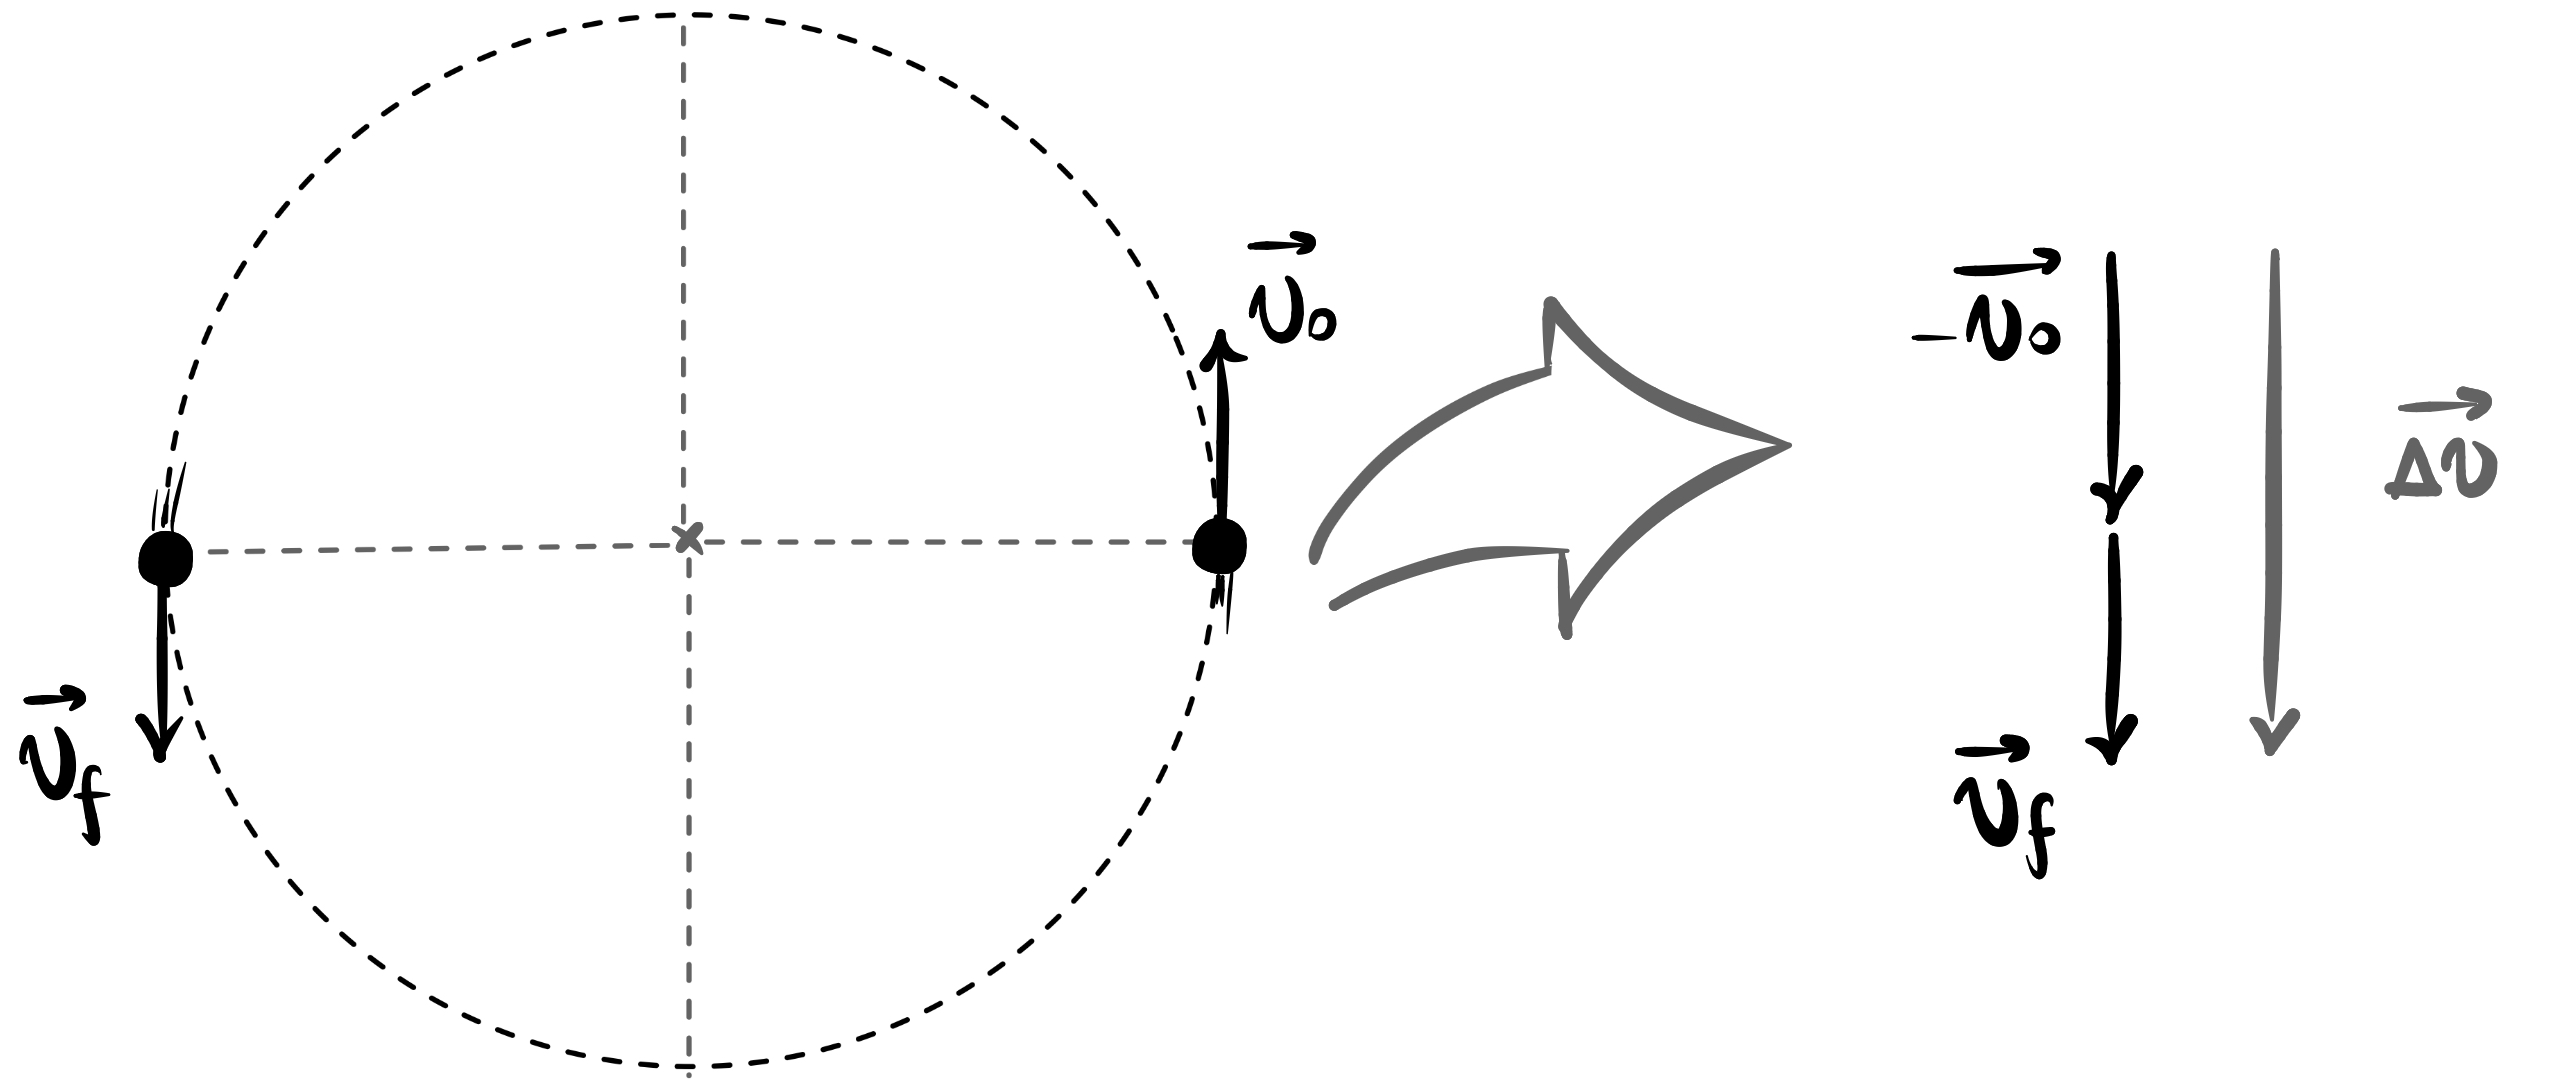
\includegraphics[width=0.6\linewidth]{imagenscinematicavetorial/fig_cinvet_aceleracaovetorialmediaexemplo0101.jpeg}
\captionof{figure}{}
\label{fig_cinvet_aceleracaovetorialmediaexemplo0101}
} 
    
    
    À direita na figura tem o esboço do cálculo de $\Delta \vec{v}=\vec{v}_f-\vec{v}_0,$ que, como se vê, terá módulo igual à soma dos módulos de $\vec{v}_0$ e $\vec{v}_f$, ou seja, $|\Delta \vec{v}|=10+10=20$m/s, de modo que a aceleração vetorial média é, neste intervalo, dada por

    $$ | \vec{a}_m|= \dfrac{|\Delta \vec{v}|}{\Delta t}= \dfrac{20 \text{ m/s}}{6\text{ s}} \implies \boxed{| \vec{a}_m|=\dfrac{10}{3}\text{ m/s$^2$}.}$$
     



   \item [(c)] Agora o intervalo de tempo é $\Delta t = t_2-t_1=6-3=3$s, de modo que a partícula terá completado um quarto de volta, situação ilustrada na Figura \ref{fig_cinvet_aceleracaovetorialmediaexemplo0102}.

{
\centering
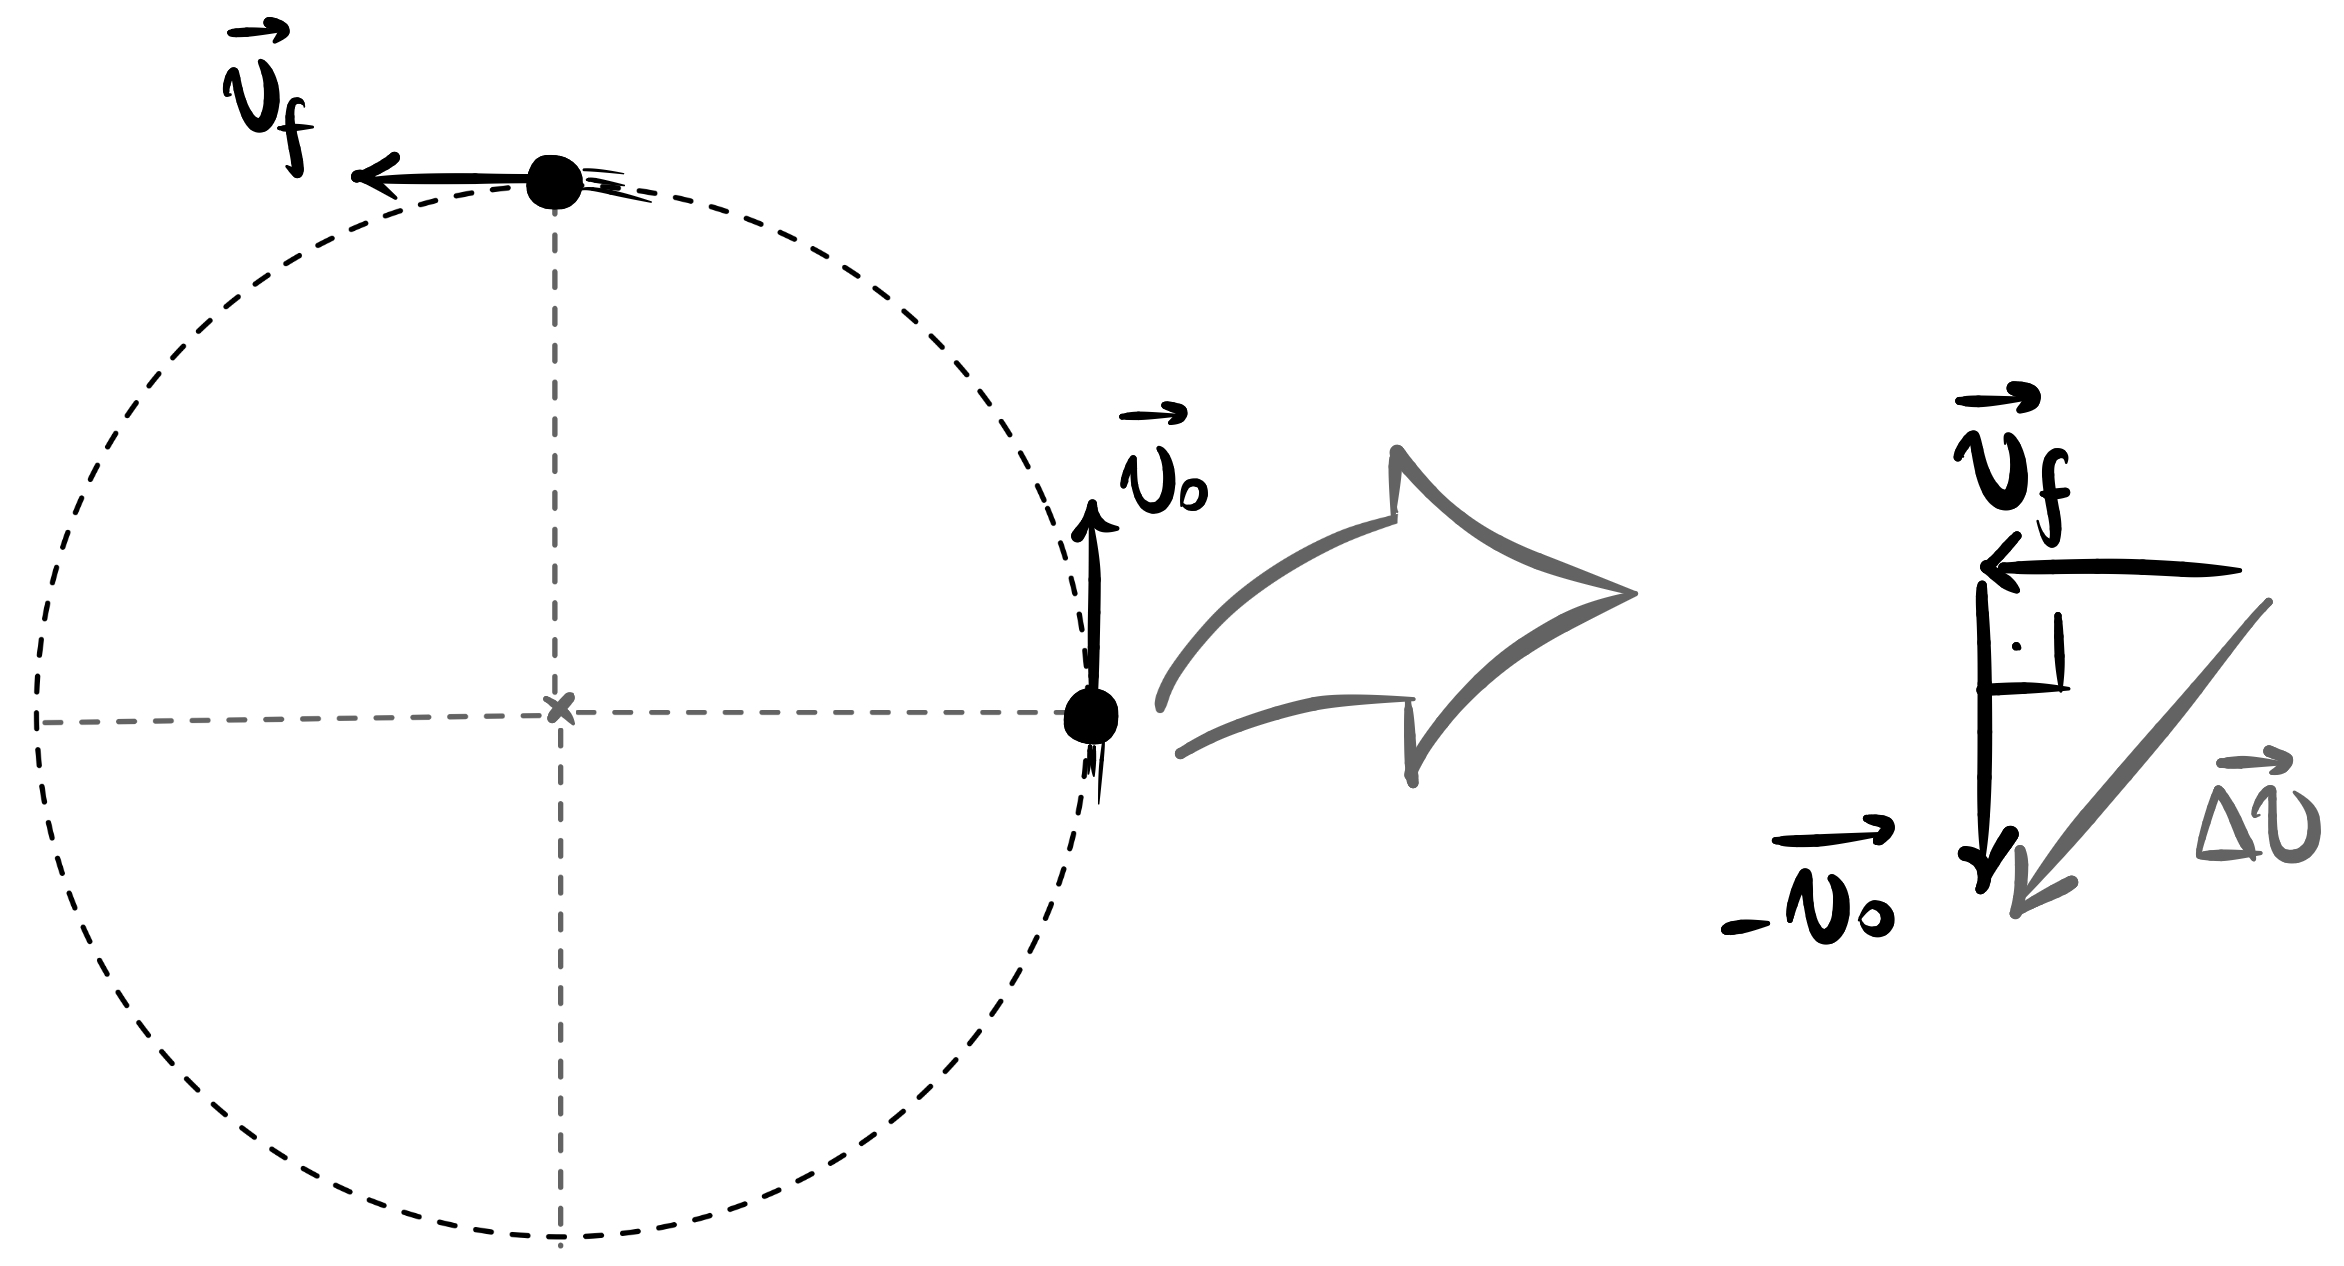
\includegraphics[width=0.6\linewidth]{imagenscinematicavetorial/fig_cinvet_aceleracaovetorialmediaexemplo0102.jpeg}
\captionof{figure}{}
\label{fig_cinvet_aceleracaovetorialmediaexemplo0102}
} 

Na parte direita da figura vemos o esboço do cálculo de $\Delta \vec{v}$, cujo módulo pode ser obtido pelo Teorema de Pitágoras:

$$ |\Delta \vec{v}|^2 = 10^2+10^2 \implies  |\Delta \vec{v}|=10\sqrt 2 \text{ m/s},$$

\noindent de modo que a aceleração vetorial média, neste intervalo, tem módulo

$$ | \vec{a}_m|= \dfrac{|\Delta \vec{v}|}{\Delta t}= \dfrac{10\sqrt 2 \text{ m/s}}{3\text{ s}} \implies \boxed{| \vec{a}_m|=\dfrac{10\sqrt2}{3}\text{ m/s$^2$}.}$$

 \item [(d)] O último intervalo de tempo é $\Delta t = t_2-t_1=5-3=2$s, de modo que a partícula terá completado $\sfrac{2}{12}=\sfrac{1}{6}$ de volta, o que significa ter girado $\sfrac{360^\circ}{6}=60^\circ$, situação ilustrada na Figura \ref{fig_cinvet_aceleracaovetorialmediaexemplo0103}.

{
\centering
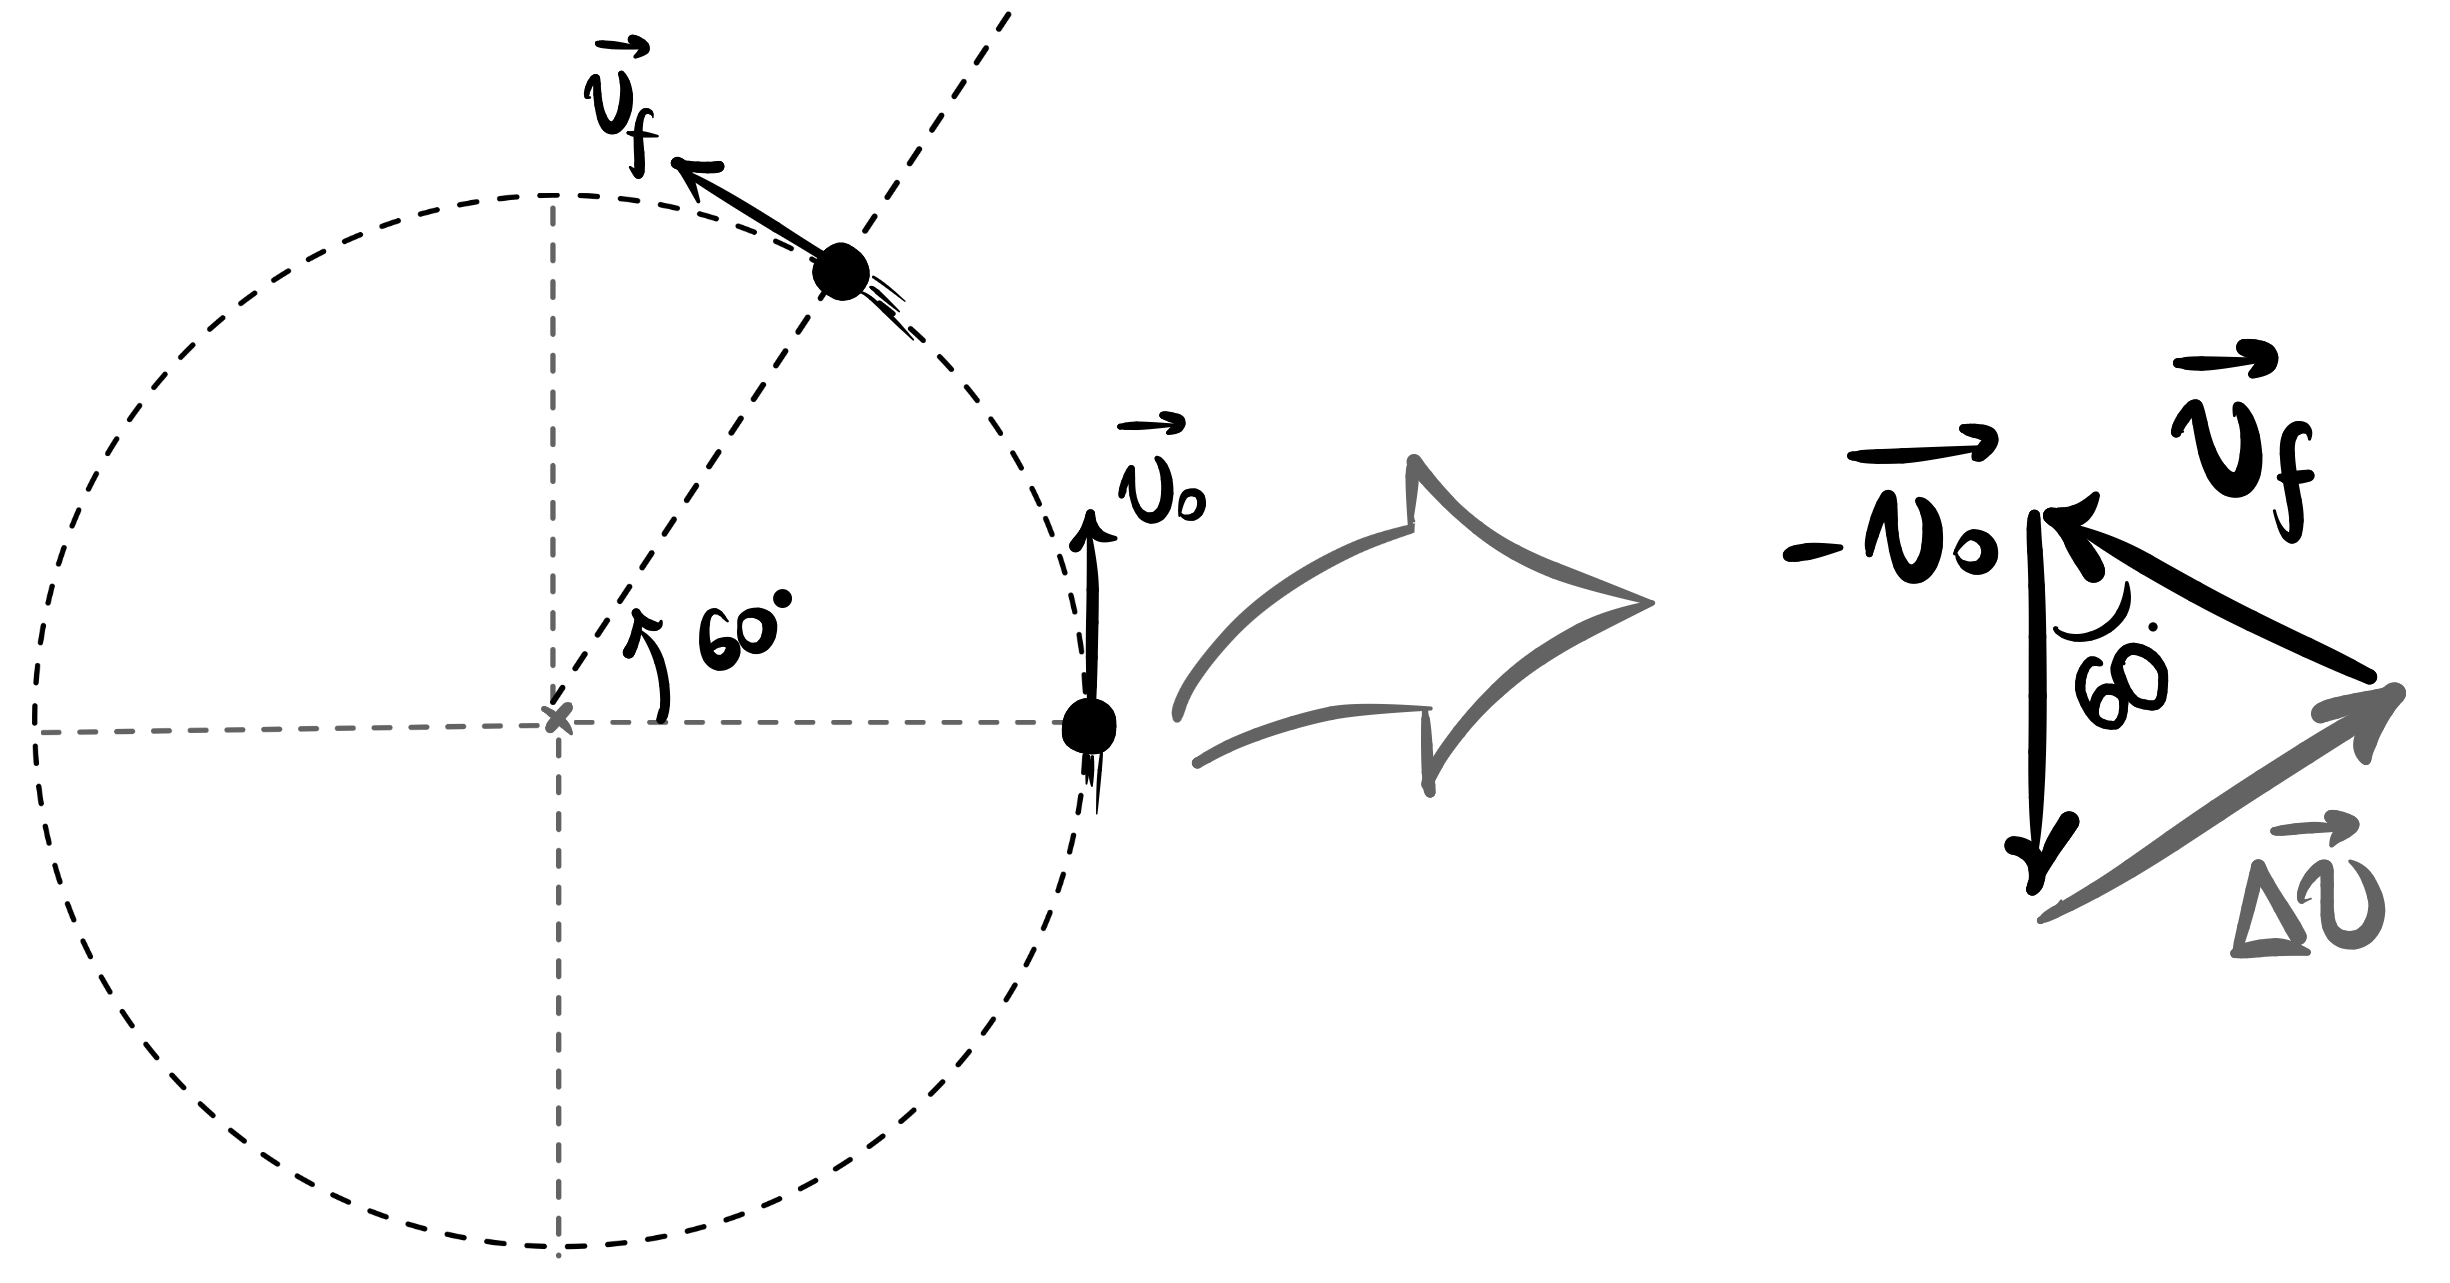
\includegraphics[width=0.6\linewidth]{imagenscinematicavetorial/fig_cinvet_aceleracaovetorialmediaexemplo0103.jpeg}
\captionof{figure}{}
\label{fig_cinvet_aceleracaovetorialmediaexemplo0103}
} 

Na parte direita da figura vemos o esboço do cálculo de $\Delta \vec{v}$, cujo módulo pode ser obtido observando que, em tal triângulo, os lados de tamanhos $|\vec{v}_0|$ e $|-\vec{v}_f|$ são iguais, de modo que os seus ângulos opostos também devem o ser -- o triângulo é isósceles. Como já temos $60^\circ$ para o ângulo de cima, cada ângulo da base precisa ter $\sfrac{(180^\circ-60^\circ)}{2}=60^\circ$, de modo que o triângulo é, na verdade, equilátero. 

Logo, temos que $|\Delta \vec{v}|=|\vec{v}_0|=|-\vec{v}_f|=10 \text{ m/s}$, de modo que a aceleração vetorial média, neste intervalo, tem módulo

$$ | \vec{a}_m|= \dfrac{|\Delta \vec{v}|}{\Delta t}= \dfrac{10 \text{ m/s}}{2\text{ s}} \implies \boxed{| \vec{a}_m|=5\text{ m/s$^2$}.}$$
     
     
    
\end{enumerate}

  
\end{exemplo}


\vspace{0.3cm}






\begin{exemplo}[Nível III]

Considere uma partícula que executa um movimento circular, de raio $R$, mantendo o módulo da sua velocidade sempre constante. Se a partícula leva um tempo $\tau$ para completar uma volta, mostre que o módulo da sua aceleração vetorial média entre os instantes $t=0s$ e $t$ é dado por

$$ |\vec{a}_m(t)|=\dfrac{4 \pi R}{t \tau}  \sin \left( \dfrac{\pi t}{\tau} \right).$$

\resolucao


Sendo a velocidade, em módulo, sempre constante, podemos computá-la por meio de $v=\sfrac{d}{t},$ e, para uma volta completa, teremos

$$ v=\dfrac{2 \pi R}{\tau}.$$

Seja $\theta$ o ângulo de giro para o intervalo de tempo $t$. Logo, tem-se 

$$ \dfrac{\theta}{t} = \dfrac{2 \pi}{\tau} \implies \theta = \dfrac{2 \pi t}{\tau}.$$

{
\centering
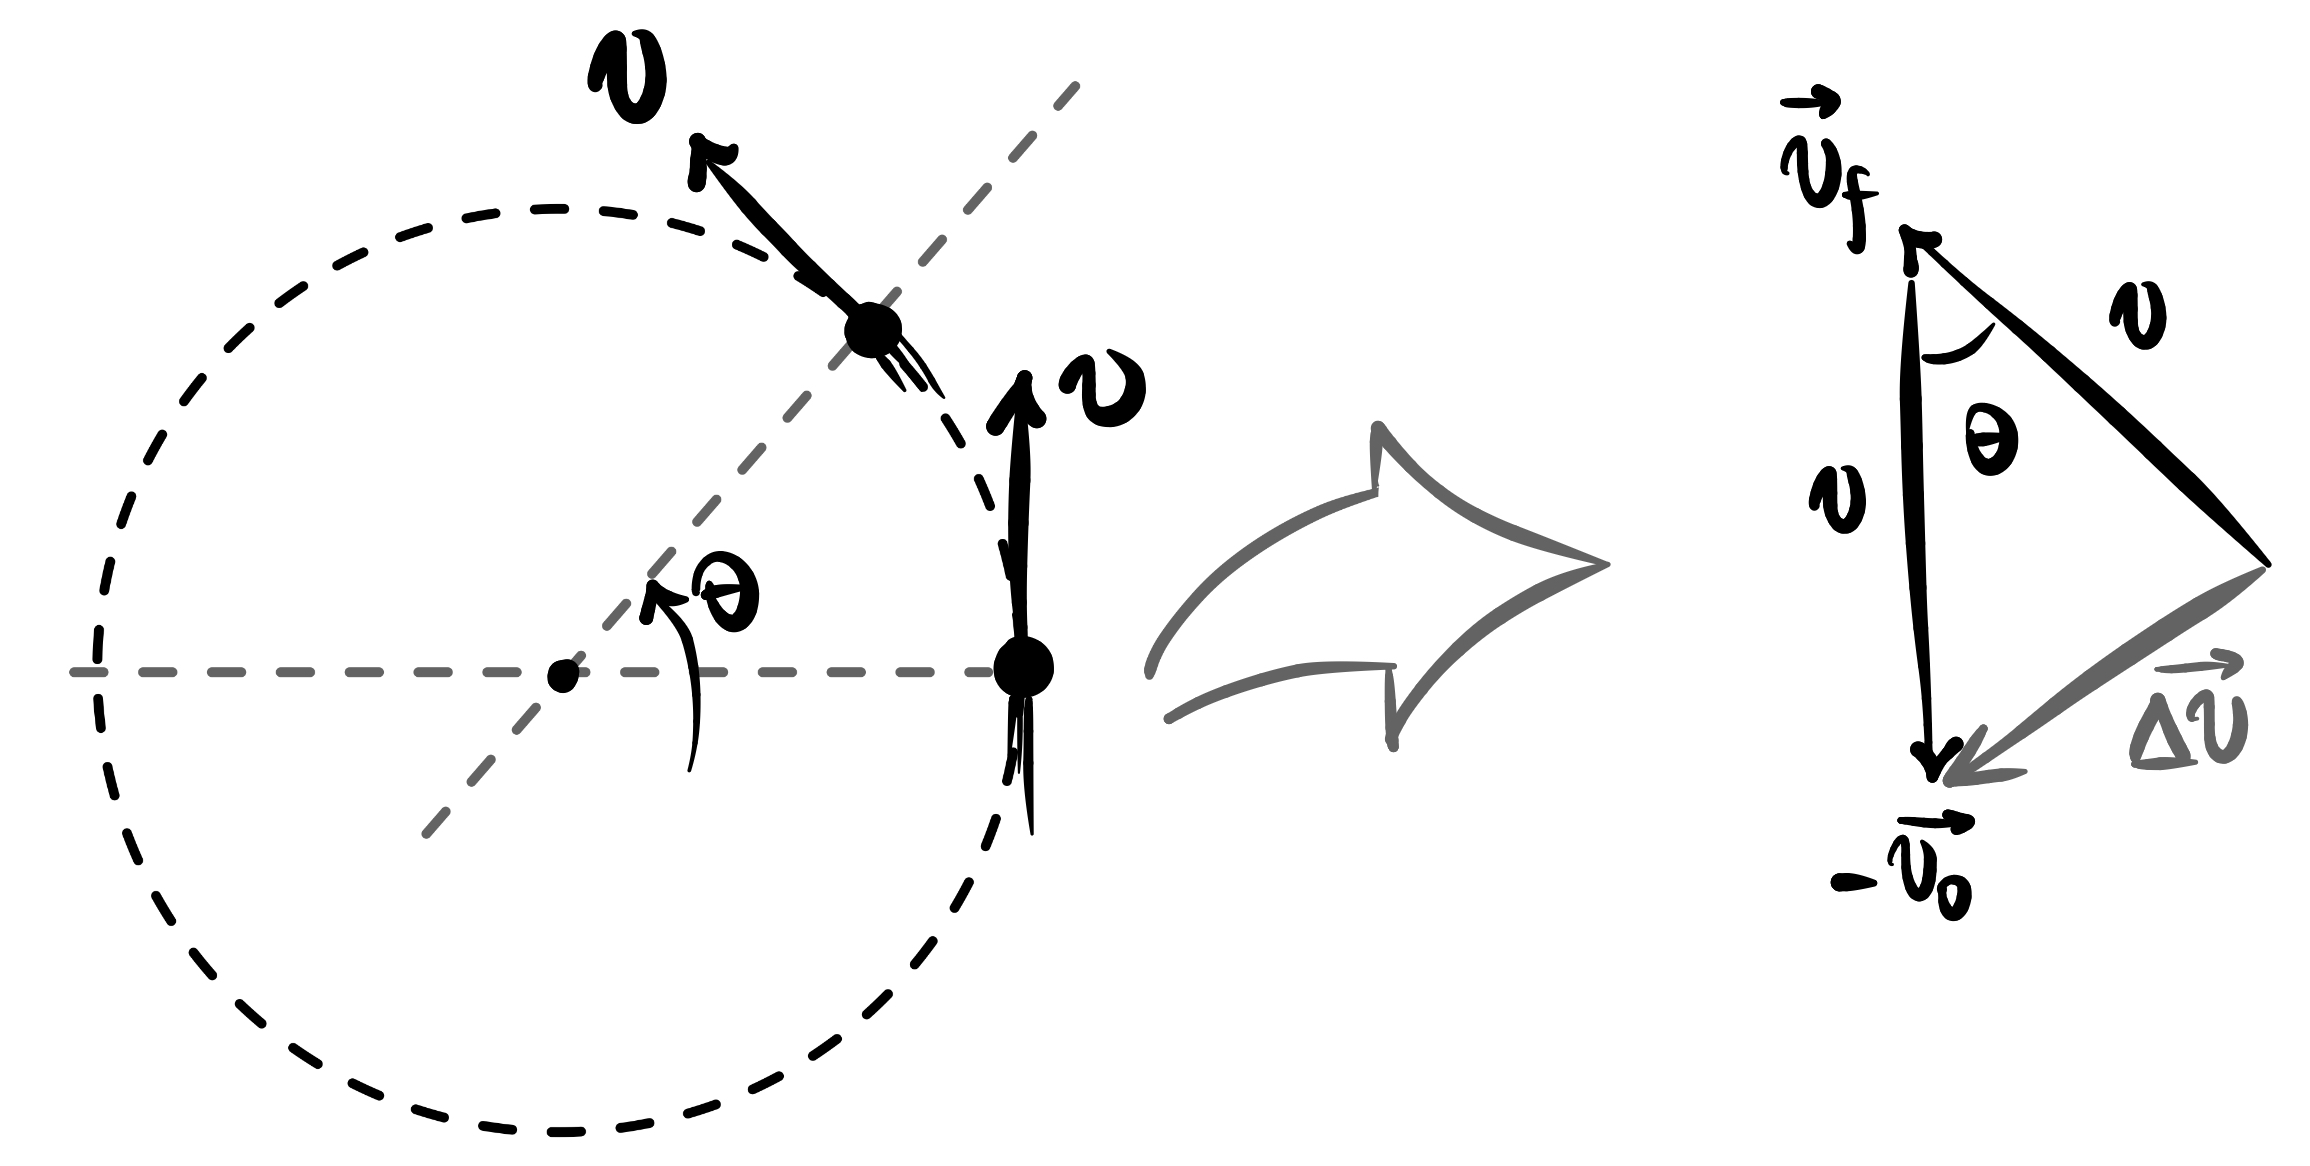
\includegraphics[width=0.5\linewidth]{imagenscinematicavetorial/fig_cinvet_aceleracaovetorialexemplonivel3.jpeg}
\captionof{figure}{}
\label{fig_cinvet_aceleracaovetorialexemplonivel3}
} 

A Figura \ref{fig_cinvet_aceleracaovetorialexemplonivel3} ilustra a situação e também o esboço dos vetores para o cálculo de $\Delta \vec{v}=\vec{v}_f-\vec{v}_0.$ Por meio da aplicação da Lei dos Cossenos no triângulo da figura, teremos:

 $$ |\Delta \vec{v}|^2= v^2+v^2 - 2 \cdot v \cdot v \cdot \cos \theta,$$

 \noindent que, por meio da fórmula do arco metade $\sin^2 \theta = \sfrac{(1-\cos \theta)}{2},$ nos leva a

 $$ |\Delta \vec{v}| = 2v \sin \left( \dfrac{\theta}{2} \right). $$



Assim, a aceleração vetorial média terá módulo, no intervalo de tempo $t$, dado por

$$ |\vec{a}_m| = \dfrac{ |\Delta \vec{v}|}{\Delta t} = \dfrac{ 2v \sin \left( \dfrac{\theta}{2} \right)}{t},$$

\noindent e, usando os valores de $\theta$ e $v$ calculados anteriormente em termos dos valores fornecidos, somos levados a

$$ \boxed{|\vec{a}_m(t)|=\dfrac{4 \pi R}{t \tau} \sin \left( \dfrac{\pi t}{\tau} \right),}$$

\noindent como queríamos demonstrar.\\

Sugerimos ao leitor que insira os valores de $t$ como sendo um período, meio período e um quarto de período para comparar os resultados com aqueles do exemplo anterior.

  
\end{exemplo}

\vspace{0.3cm}




\begin{secnivel}[Aceleração Centrípeta]{I}{Aceleração Centrípeta}
  
  \eqLdois{dem}{cinvet_eq_aceleracaocentripeta}{a_c=\dfrac{v^2}{r}}

\end{secnivel}








\secgfe{De onde vem}

Nos exemplos resolvidos da Equação \eqref{cinvet_eq_aceleracaovetorialmedia} ficou claro que, mesmo em um movimento no qual a velocidade não muda em valor, isto é, o tamanho do vetor é sempre constante, deve existir algum tipo de aceleração caso a direção desse vetor mude, ou seja, caso o movimento faça algum tipo de curva. O melhor movimento para avaliarmos isso é justamente aquele usado em tais exemplos: o Movimento Circular Uniforme (MCU).

O fato de ser um movimento uniforme implica que o valor (módulo) da velocidade do objeto é constante; logo, não existe a aceleração que até então conhecíamos: a aceleração que faz variar o valor da velocidade -- aceleração escalar. Contudo, no MCU, a direção do vetor velocidade muda o tempo inteiro, uma vez que este é sempre tangente à trajetória. Logo, deve haver aqui algum tipo de aceleração -- aquela responsável por alterar a direção do vetor velocidade, e não o seu módulo. À \textbf{componente} da aceleração que faz isso damos o nome de aceleração centrípeta, representada por $a_c.$

Logo, é como se a aceleração vetorial $\vec{a}$ fosse composta de duas partes, a aceleração centrípeta $\vec{a}_c$ e a aceleração tangencial $\vec{a}_t$. \footnote{Essa última é justamente a aceleração que faz variar o módulo da velocidade e coincide com o valor da conhecida aceleração escalar. Discutiremos tal componente em uma seção própria a ela.} Logo, a aceleração vetorial é

$$\boxed{ \vec{a} = \vec{a}_c + \vec{a}_t.}$$

Contudo, no MCU, como o valor da velocidade nunca muda, a aceleração $a_t$ será nula, logo

$$ \vec{a} = \vec{a}_c + \cancelto{0}{\vec{a}_t} \implies  \boxed{ \vec{a} = \vec{a}_c,}$$

\noindent ou seja, se calcularmos a aceleração vetorial usando a Equação \eqref{cinvet_eq_aceleracaovetorialmedia}, ela irá coincidir, no caso do MCU, com a aceleração centrípeta, que é quem queremos encontrar. Este será o caminho para construirmos a Equação \eqref{cinvet_eq_aceleracaocentripeta}. 

Considere, portanto, o MCU representado na Figura \ref{fig_cinvet_demonstracaoacentripeta01}, em que a circunferência tem raio $R$ e o valor da velocidade da partícula é $v$. Considere a partícula se movendo entre os pontos $A$ e $B,$ nos quais sua velocidade é dada pelos vetores $\vec{v}_1$ e $\vec{v}_2,$ respectivamente. Sendo o movimento uniforme, o módulo de tais vetores é o mesmo, isto é

$$ |\vec{v}_1| = |\vec{v}_2| = v.$$


{
\centering
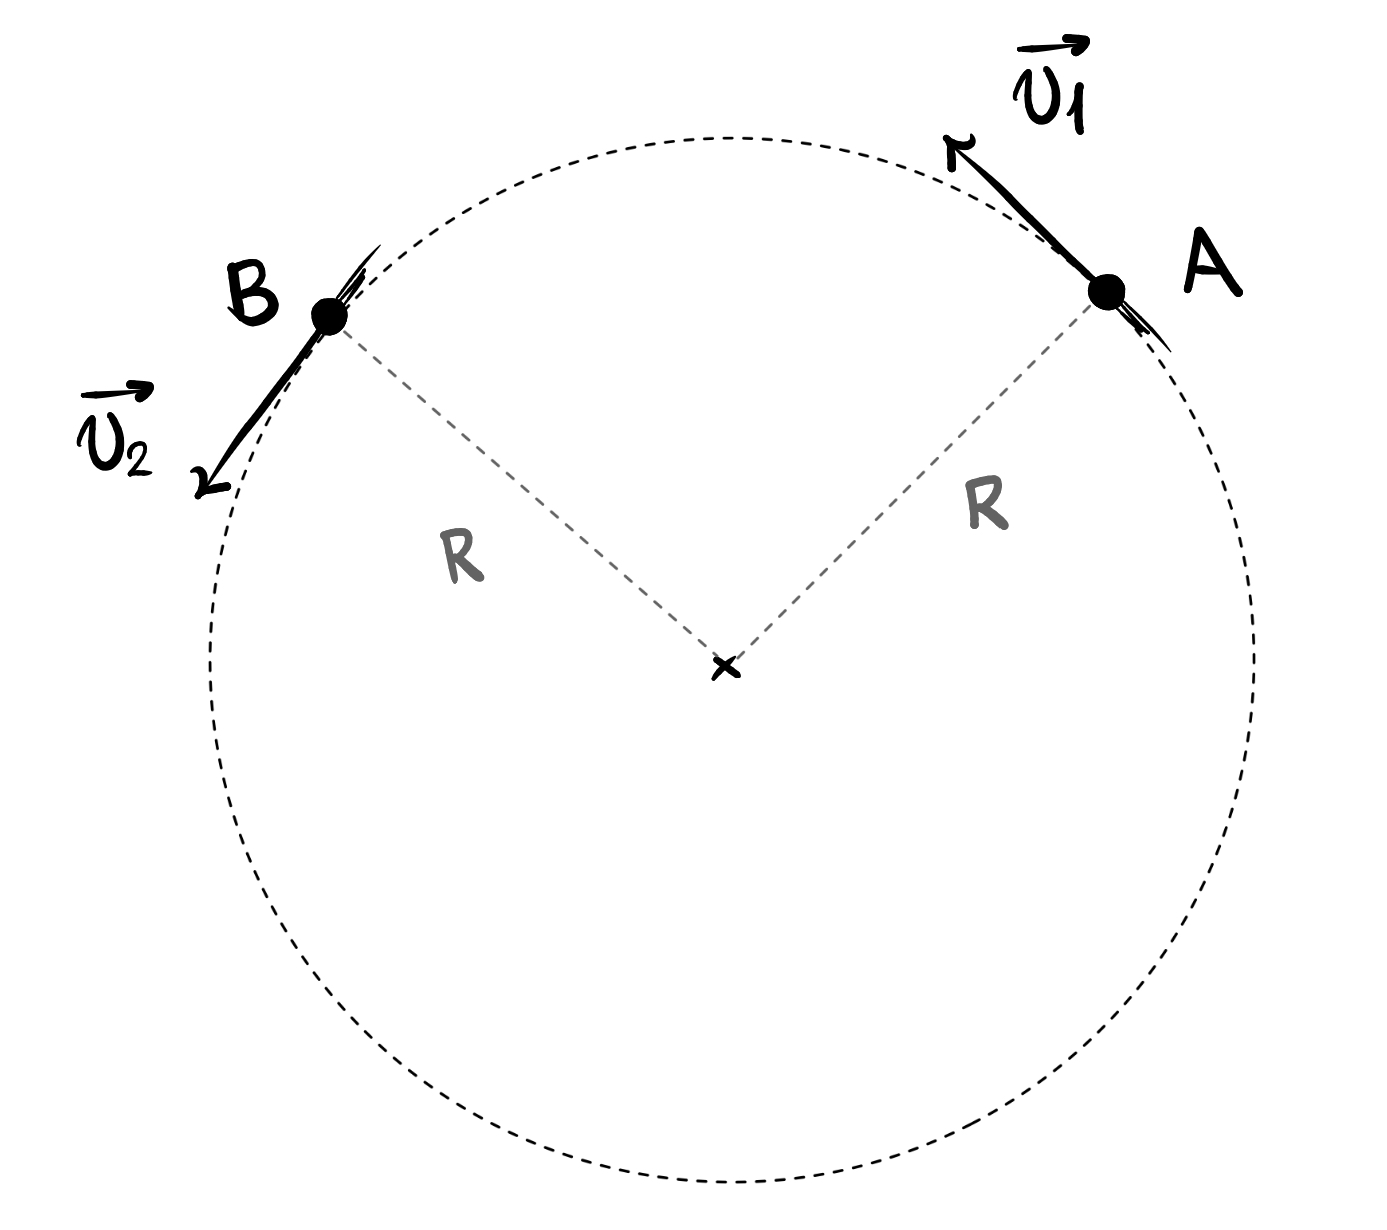
\includegraphics[width=0.35\linewidth]{imagenscinematicavetorial/demonstracaoacentripeta01.jpeg}
\captionof{figure}{Movimento Circular Uniforme: o módulo dos vetores $\vec{v}_1$ e $\vec{v}_2$ é o mesmo.}
\label{fig_cinvet_demonstracaoacentripeta01}
} 

\vspace{0.3cm}

Vimos que, neste caso, a aceleração centrípeta coincidirá com a aceleração vetorial, que é computada pela Equação \eqref{cinvet_eq_aceleracaovetorialmedia} por meio de:

$$ \vec{a} = \dfrac{\Delta \vec{v}}{\Delta t.}$$

A Figura \ref{fig_cinvet_demonstracaoacentripeta02} mostra o esboço do cálculo do vetor $\Delta \vec{v} = \vec{v}_2 -  \vec{v}_1 $. Na primeira imagem projetamos em linha pontilhada a direção dos dois vetores e os arrastamos, ao longo de tais linhas, de modo a desenhá-los com a origem de um deles coincidindo com a extremidade do outro. O vetor $\vec{v}_1$ teve seu sentido invertido para fazermos a soma $\Delta \vec{v} = \vec{v}_2 +  (-\vec{v}_1), $ que é um vetor que vai da origem do primeiro à extremidade do último, como a segunda imagem indica.


\vspace{0.3cm}
{
\centering
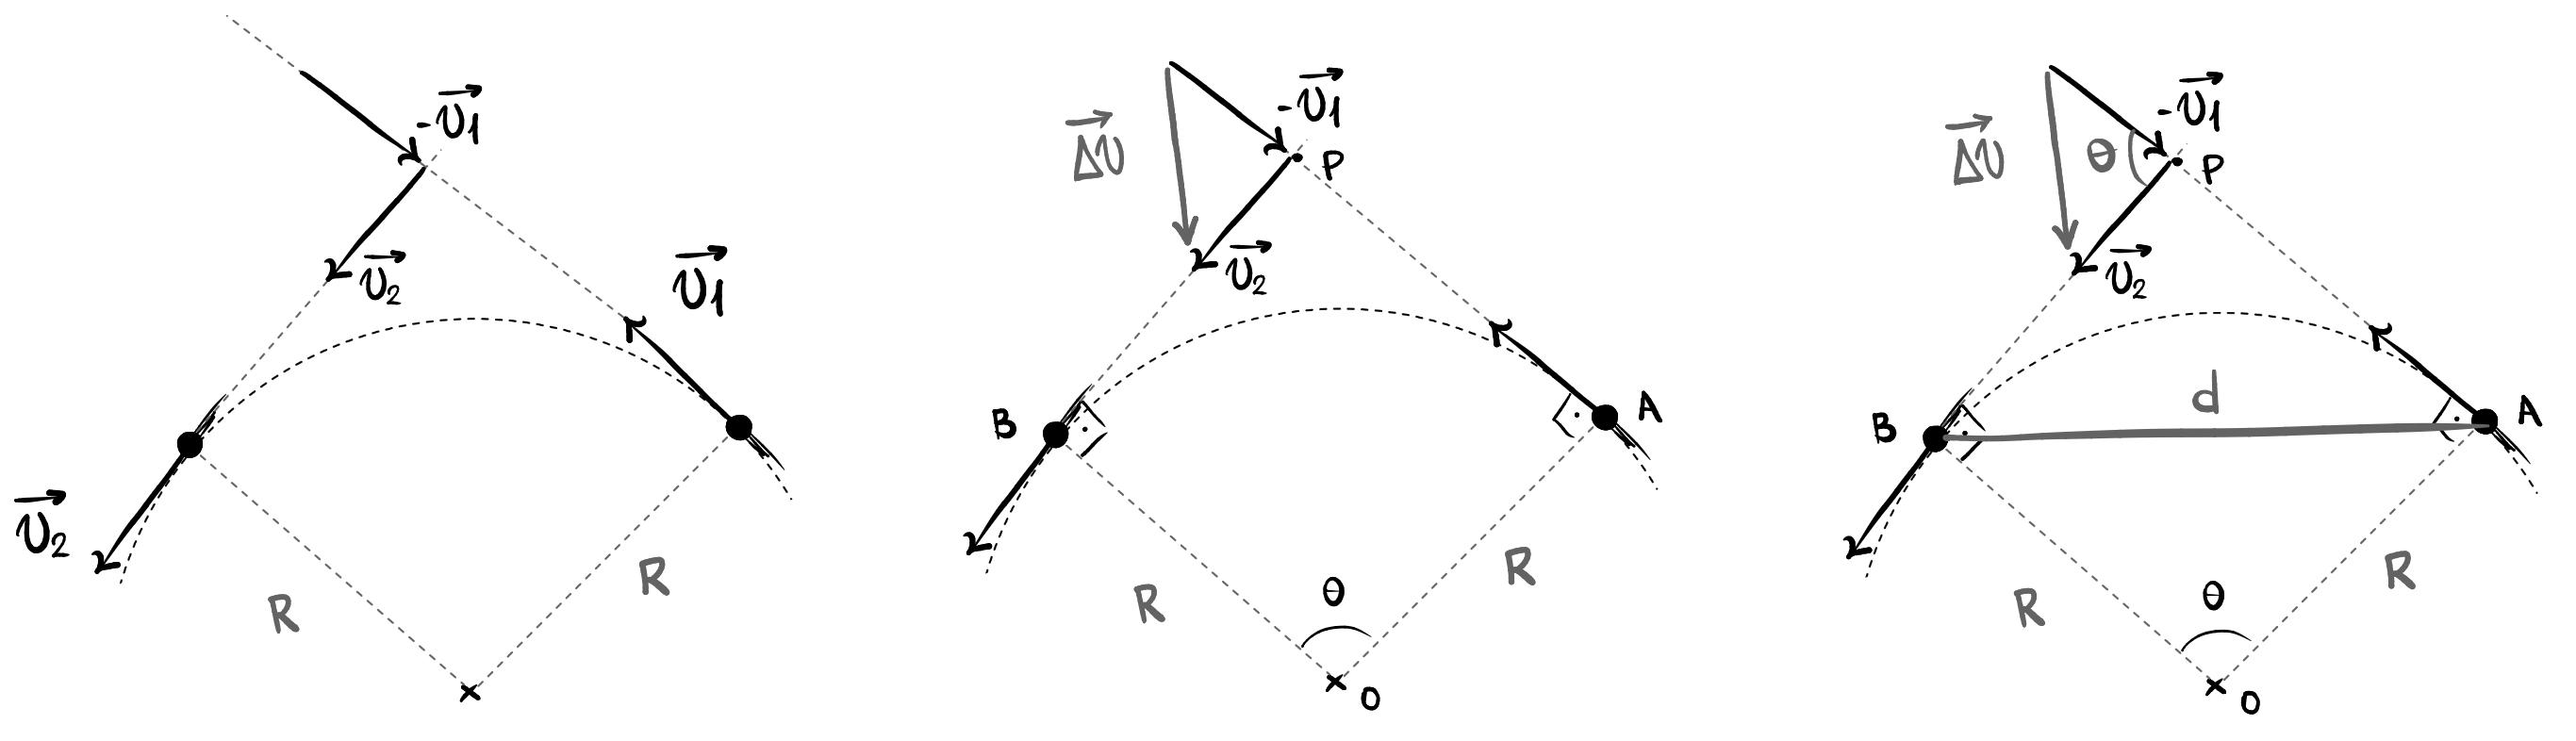
\includegraphics[width=1.0\linewidth]{imagenscinematicavetorial/demonstracaoacentripeta02.jpeg}
\captionof{figure}{Cálculo do vetor $\Delta \vec{v}$.}
\label{fig_cinvet_demonstracaoacentripeta02}
} 
\vspace{0.3cm}

Note, ainda na segunda imagem da Figura \ref{fig_cinvet_demonstracaoacentripeta02}, que os ângulos $\angle OAP$ e $\angle OBP$ são retos, haja vista que a velocidade é tangente à trajetória e, portanto, perpendicular ao raio. Logo, como os ângulos internos do quadrilátero $AOBP$ devem totalizar $360^\circ$, concluímos que o ângulo $\angle APB$ deve medir $180^\circ - \theta,$ de onde obtemos que o ângulo adjacente à ele, que é seu suplementar -- o ângulo entre os vetores $\vec{v}_2$ e $-\vec{v}_1$ -- terá medida igual a $\theta$, como mostra a terceira imagem da figura. Dessa terceira imagem extrairemos os triângulos $AOB$ e o triângulo formado pelos vetores, que se encontram na Figura \ref{fig_cinvet_demonstracaoacentripeta03}.

\vspace{0.3cm}

{
\centering
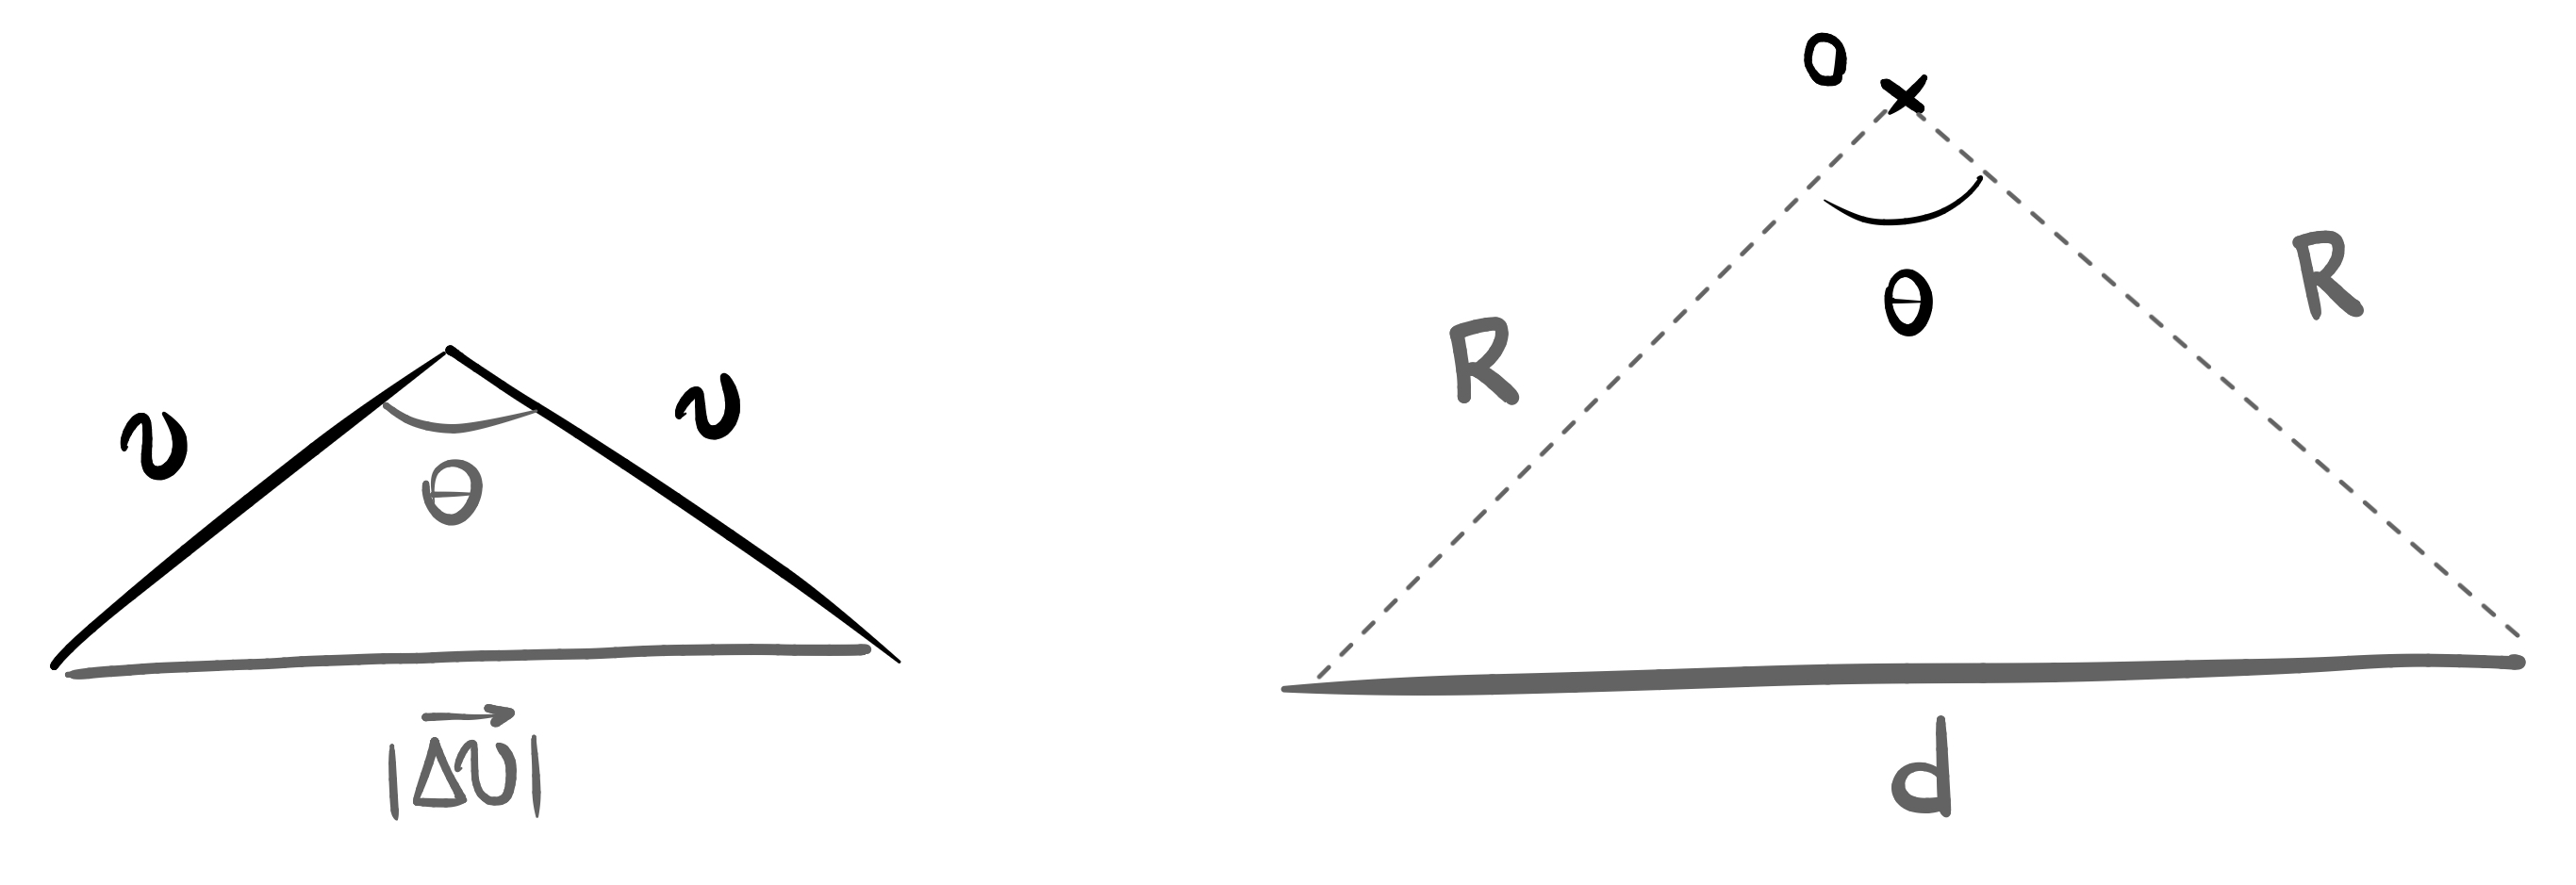
\includegraphics[width=0.6\linewidth]{imagenscinematicavetorial/demonstracaoacentripeta03.jpeg}
\captionof{figure}{O triângulo dos vetores é semelhante ao triângulo geométrico formado pelos raios e pela distância.}
\label{fig_cinvet_demonstracaoacentripeta03}
} 
\vspace{0.3cm}

Note que esses triângulos são semelhantes: ambos possuem o ângulo $\theta$ e, como os dois são isósceles, os ângulos da base também serão iguais. Logo, por semelhança de triângulos, podemos escrever que

$$ \dfrac{|\Delta \vec{v}|}{d} = \dfrac{v}{R} \implies |\Delta \vec{v}| = \dfrac{vd}{R},$$

\noindent mas, sendo o movimento uniforme, podemos escrever que $d=v\Delta t,$ de modo que somos levados a

$$ |\Delta \vec{v}| = \dfrac{v}{R} \cdot v\Delta t\implies \boxed{\dfrac{|\Delta \vec{v}|}{\Delta t} = \dfrac{v^2}{R}.} $$


Perceba que, pela definição da Equação \eqref{cinvet_eq_aceleracaovetorialmedia}, o que calculamos acima é justamente o módulo do vetor aceleração. Mas, como vimos, no MCU só existe um tipo de aceleração: a aceleração responsável por mudar a direção do vetor velocidade, ou seja, a aceleração centrípeta. Assim, temos que, para o MCU,

$$ |\vec{a}| = a_c = \dfrac{v^2}{R},$$

\noindent como queríamos demonstrar.

Sobre tal equação é importante pontuar algumas observações:

\begin{enumerate}
    \item [(i)] A Equação \eqref{cinvet_eq_aceleracaocentripeta} vale para qualquer tipo de movimento curvilíneo. Demonstramos ela nessa seção partindo do MCU para fins didáticos, uma vez que este é o movimento no qual só há aceleração centrípeta, simplificando os cálculos e a geometria.

    Para qualquer tipo de movimento que faça curva, portanto, existirá uma aceleração, calculada pela Equação \eqref{cinvet_eq_aceleracaocentripeta}, que é responsável por fazer a mudança na direção do vetor velocidade e, portanto, possibilitar que o movimento seja curvo.

    Para o leitor curioso que pode ter se indagado a respeito do que significaria o raio $R$ na Equação \eqref{cinvet_eq_aceleracaocentripeta} no caso de um movimento que não seja circular, trataremos disso nas próximas linhas. Adianto ao nobre leitor que a discussão que se segue é um pouco mais abstrata -- de modo que pode ser pulada em uma primeira leitura.


A resposta começa com uma observação simples: olhe com atenção para
qualquer curva e, num determinado ponto $P$, tente encontrar o círculo
que melhor a ``\emph{abraça}'' naquele instante — aquele que toca a curva em
$P$ e se curva com a mesma
intensidade. Esse círculo especial é chamado de \textit{círculo
osculador} (do latim \textit{osculari}, ``beijar''), e seu raio recebe
o nome de \textit{raio de curvatura} da trajetória naquele ponto.

\vspace{0.3cm}
{
\centering
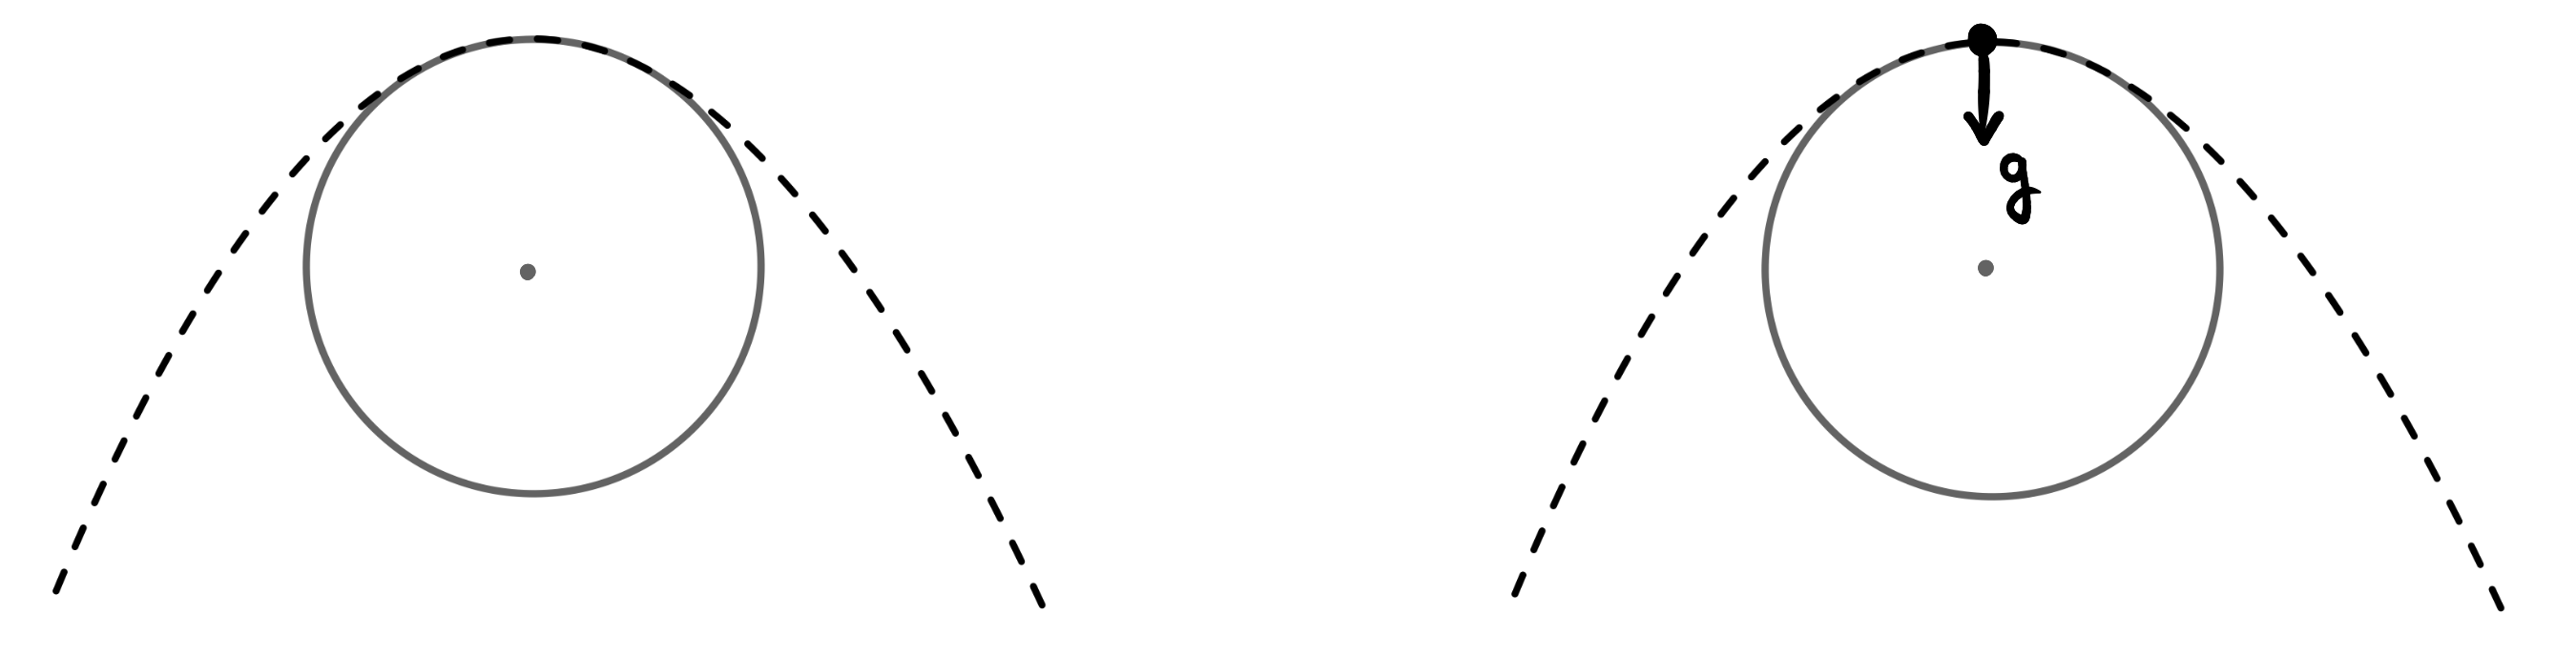
\includegraphics[width=0.75\linewidth]{imagenscinematicavetorial/circunferenciaoscular.png}
\captionof{figure}{A circunferência oscular.}
\label{fig_cinvet_circoscular}
} 
\vspace{0.3cm}

A Figura \ref{fig_cinvet_circoscular} ilustra a ideia. No ponto $P$, o círculo tracejado e a
trajetória se tocam tão intimamente que, visto de perto, seria
impossível distingui-los — eles compartilham a mesma tangente e a
mesma curvatura. Um pouco além de $P$, porém, os dois caminhos se
dividem: a trajetória segue o seu curso, e o círculo segue o seu.

O que torna isso poderoso é que a Equação \eqref{cinvet_eq_aceleracaocentripeta} continua válida em
qualquer ponto de qualquer trajetória curva, desde que $R$ seja
interpretado como esse raio de curvatura local:
%
\begin{equation}
    a_c = \frac{v^2}{R}.
    \nonumber
\end{equation}
%
Quando a curva é muito fechada, o círculo osculador é pequeno, $R$ é
pequeno, e a aceleração centrípeta necessária é grande. Quando a
trajetória é quase reta, o círculo osculador é enorme — no limite, uma
linha reta corresponde a um círculo de raio infinito —, e $a_c \to 0$.

Considere, por exemplo, no topo da parábola, como a
segunda imagem da Figura \ref{fig_cinvet_circoscular} ilustra. Naquele instante, a velocidade é puramente
horizontal e a única aceleração que age sobre o projétil é a gravidade
$g$, apontando verticalmente para baixo — exatamente em direção ao
centro $C$ do círculo osculador. A gravidade, portanto, desempenha o
papel de aceleração centrípeta, e isso é suficiente para determinar o
raio de curvatura da parábola naquele ponto.




    

    \item [(ii)] O leitor mais atento pode ter se sentido desconfortável quando usamos que o segmento de tamanho $d$, na terceira imagem da Figura \ref{fig_cinvet_demonstracaoacentripeta02}, fosse igual à distância percorrida pela partícula. A distância $d$, na verdade, é igual ao comprimento do arco pontilhado de circunferência -- essa é a trajetória que o corpo percorre. Já a distância em linha reta entre os pontos $A$ e $B$ é o deslocamento, que, em geral, é diferente da distância. Contudo, como mostra a Figura \ref{fig_cinvet_demonstracaoacentripeta04}, para intervalos de tempo muito pequenos a distância percorrida -- a linha pontilhada -- fica cada vez mais próxima do deslocamento -- linha cheia -- de modo que essas duas grandezas coincidem se o tempo for suficientemente pequeno, como discutimos na construção da Equação \eqref{cinvet_eq_velocidadevetorialmedia}.

\vspace{0.3cm}
{
\centering
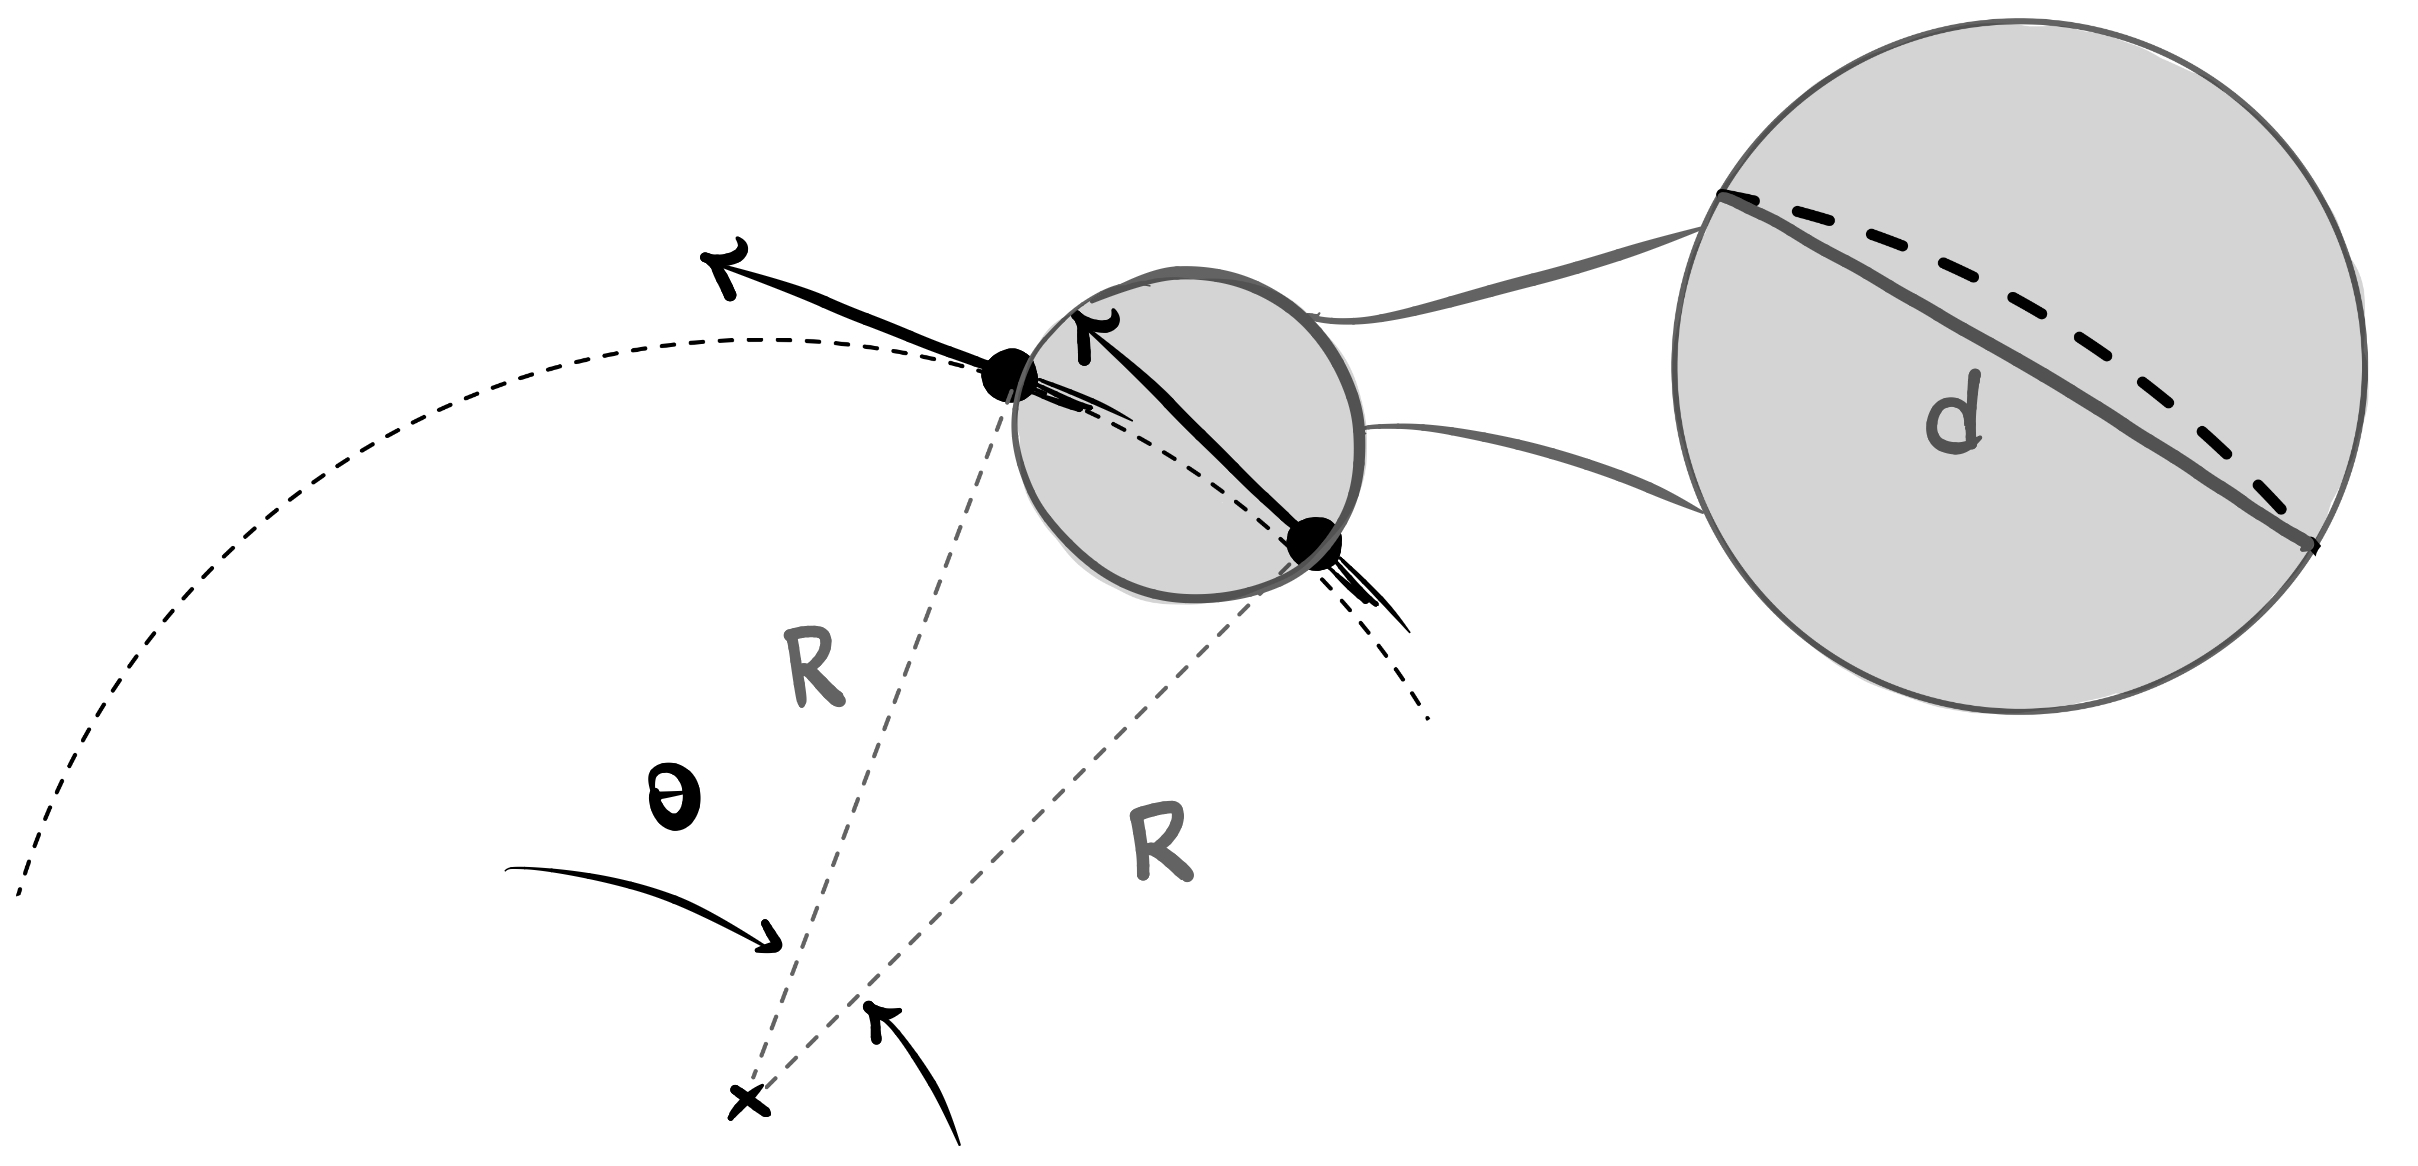
\includegraphics[width=0.6\linewidth]{imagenscinematicavetorial/demonstracaoacentripeta04.jpeg}
\captionof{figure}{O deslocamento e a distância percorrida coincidem quando o intervalo de tempo é muito pequeno.}
\label{fig_cinvet_demonstracaoacentripeta04}
} 
\vspace{0.3cm}

Como queremos calcular a aceleração vetorial em um ponto específico da trajetória do corpo, a ideia é calcular a aceleração vetorial média, porém usando um intervalo de tempo tão pequeno que, como quase não deu tempo da partícula se mover, estaremos praticamente calculando a aceleração naquele instante. 

      \item [(iii)]  Com base na ideia anterior, como vamos avaliar um intervalo de tempo muito curto para obter a aceleração da partícula em um instante específico -- e não uma média entre dois instantes distantes -- o ângulo de abertura $\theta$ dos triângulos da Figura \ref{fig_cinvet_demonstracaoacentripeta03} será muito pequeno. A própria Figura \ref{fig_cinvet_demonstracaoacentripeta04} já evidencia isso: em um intervalo de tempo curto a partícula se move muito pouco, de modo que a abertura angular $\theta$ é pequena. 

      Na verdade a abertura angular é tão pequena, mas tão pequena, que o ângulo $\theta$ é praticamente zero, como mostra a Figura \ref{fig_cinvet_acentripetaapontaparacentro1}. No caso limite, como a última imagem tenta mostrar, os ângulos da base do triângulo isósceles tendem a $90^\circ.$ Para que isso fique claro, sendo $\alpha$ o valor de cada ângulo, precisamos que 
       
       $$ \alpha + \alpha + \theta = 180^\circ,$$

       \noindent contudo, sendo $\theta$ praticamente zero, vemos que
       
  $$ \alpha + \alpha + \cancelto{0}{\theta} = 180^\circ \implies  \boxed{\alpha =90^\circ.}$$
  
\vspace{0.3cm}
{
\centering
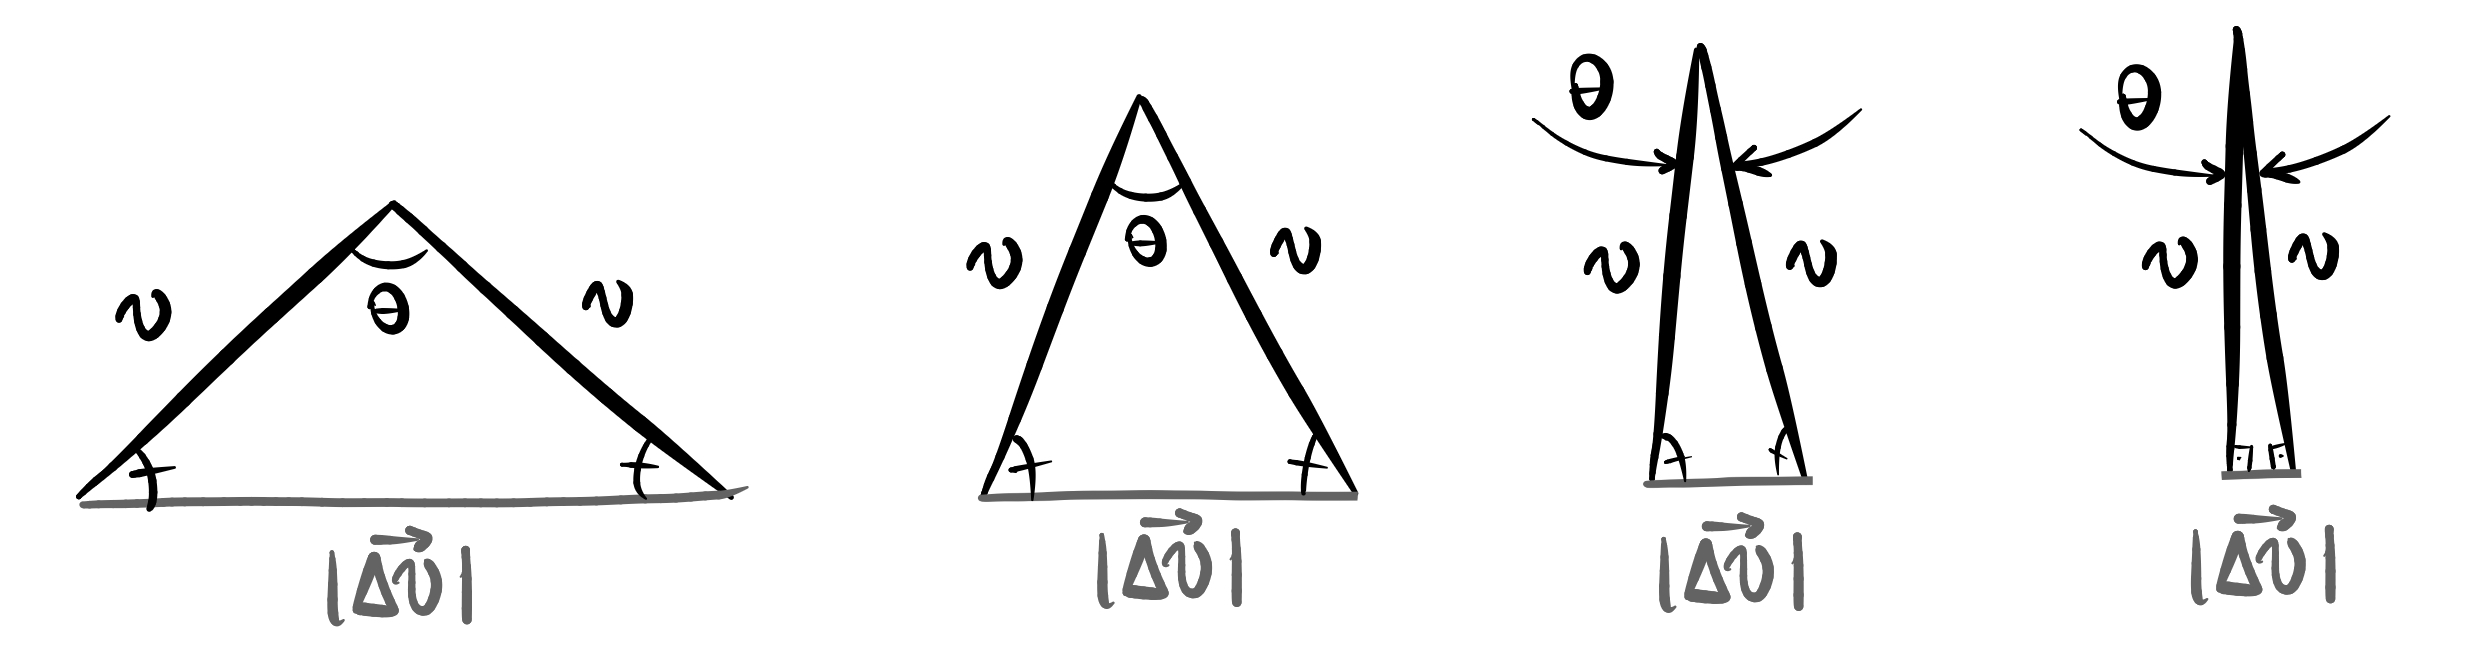
\includegraphics[width=0.8\linewidth]{imagenscinematicavetorial/acentripetaapontaparacentro1.jpeg}
\captionof{figure}{Quando o intervalo de tempo é muito curto a abertura angular é muito pequena, de modo que os ângulos iguais do triângulo tendem a $90^\circ$ cada.}
\label{fig_cinvet_acentripetaapontaparacentro1}
} 
\vspace{0.3cm}

Contudo, lembre-se que triângulos da Figura \ref{fig_cinvet_acentripetaapontaparacentro1} representam, na verdade, o triângulo dos vetores $-\vec{v}_1$, $\vec{v}_2$ e $\Delta \vec{v}$ da terceira imagem da Figura \ref{fig_cinvet_demonstracaoacentripeta02}. Ou seja, o ângulo $\alpha$ em questão é o ângulo entre o vetor $\Delta \vec{v}$ e o vetor velocidade da partícula (seja ele $\vec{v}_1$ ou $\vec{v}_2$, porque, como o intervalo de tempo é curto, tais vetores serão praticamente paralelos -- quase não deu tempo da velocidade mudar de direção). 

Estamos concluindo, portanto, que o vetor $\Delta \vec{v}$ é perpendicular à velocidade da partícula. Porém, sendo a aceleração vetorial dada por

$$ \vec{a} = \dfrac{\Delta \vec{v}}{\Delta t},$$

\noindent vê-se que os vetores $\vec{a}$ e ${\Delta \vec{v}}$ possuem a mesma direção e o mesmo sentido, uma vez que são múltiplos escalares um do outro (sendo tal escalar -- um intervalo de tempo -- positivo). Logo, sendo a aceleração vetorial neste contexto puramente centrípeta, a conclusão final é que

$$ \boxed{\text{ a aceleração centrípeta é perpendicular ao vetor velocidade em cada instante.}}$$

Sendo a velocidade sempre tangente à trajetória, a direção perpendicular à tangente em uma circunferência é a direção radial (direção dos raios da circunferência), de forma que a conclusão acima está dizendo que a aceleração centrípeta, portanto, sempre aponta na direção do centro da circunferência -- chamada de direção centrípeta ou direção radial. Por isso, inclusive, ela leva esse nome. A Figura \ref{fig_cinvet_acentripetaapontaparacentro2} ilustra este fato.


\vspace{0.3cm}
{
\centering
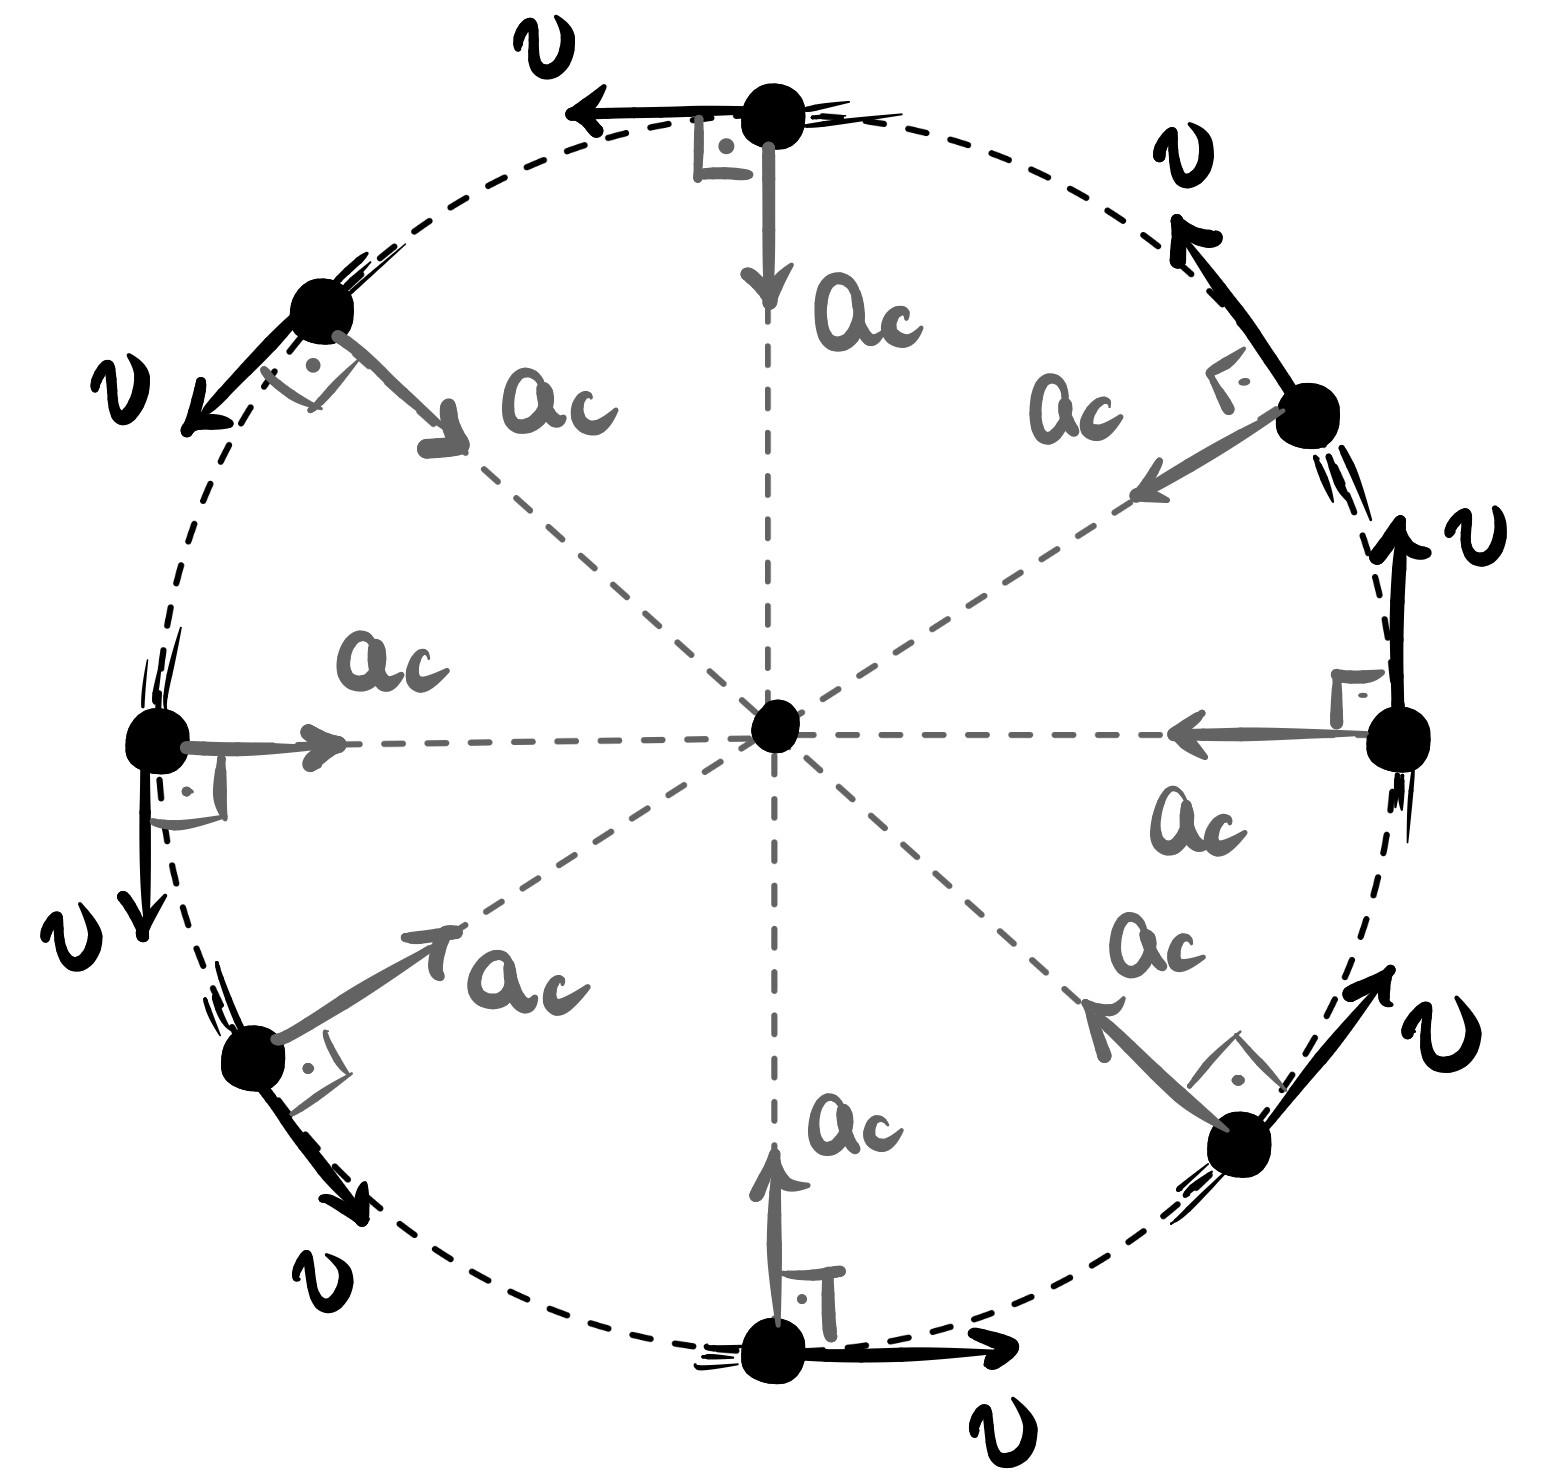
\includegraphics[width=0.4\linewidth]{imagenscinematicavetorial/acentripetaapontaparacentro2.jpeg}
\captionof{figure}{A aceleração centrípeta é sempre perpendicular à velocidade, apontando para o centro de curvatura em cada instante.}
\label{fig_cinvet_acentripetaapontaparacentro2}
} 

\end{enumerate}



\secgfe{Onde é usada}

Em praticamente qualquer contexto em que haja um movimento circular. Na verdade, o movimento sequer precisa ser circular: como a aceleração centrípeta é a responsável por alterar a direção do vetor velocidade, em absolutamente qualquer movimento que faça curva -- seja essa curva um arco de circunferência ou qualquer outra figura geométrica -- a aceleração centrípeta estará presente, garantindo que seja possível haver tal mudança de direção. Os movimentos circulares, por serem figuras geométricas mais simples, costumam ser os casos de aplicação mais comuns.

A Figura \ref{fig_cinvet_acentripetaexemplos} ilustra, para diferentes tipos de trajetórias curvilíneas, o vetor aceleração centrípeta -- sempre perpendicular à velocidade e apontando na direção radial, no sentido do centro de curvatura.

\vspace{0.3cm}
{
\centering
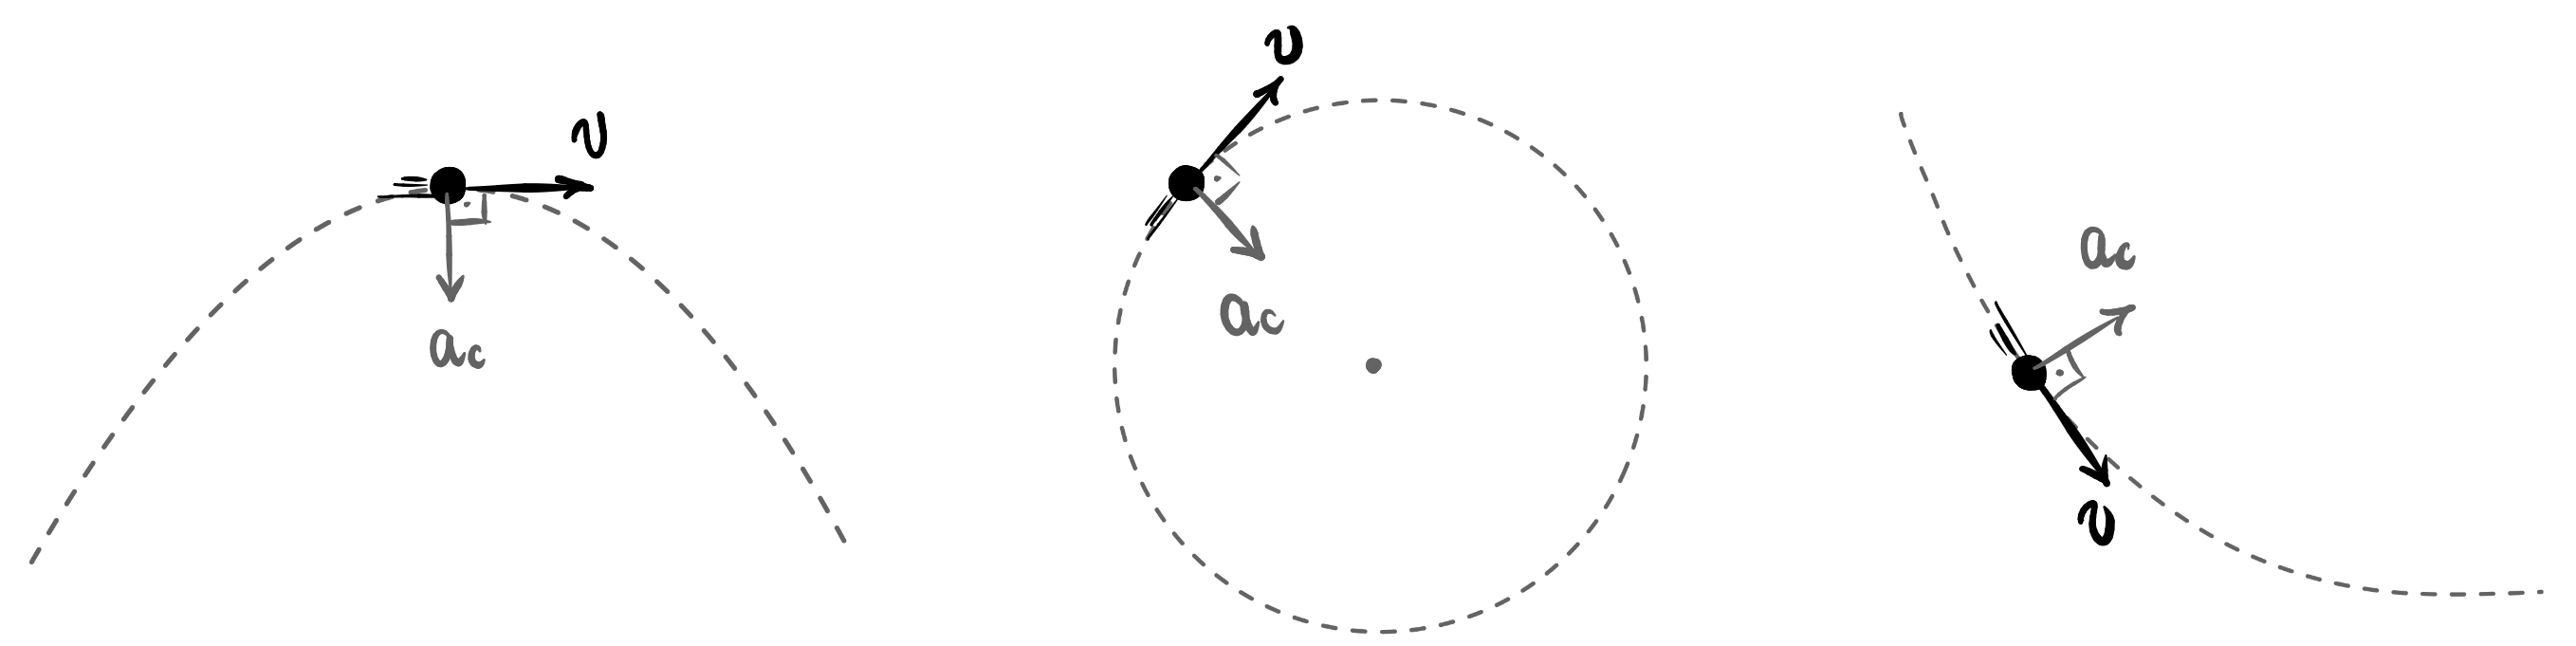
\includegraphics[width=0.8\linewidth]{imagenscinematicavetorial/acentripetaexemplos.jpeg}
\captionof{figure}{O vetor aceleração centrípeta em diferentes tipos de trajetória.}
\label{fig_cinvet_acentripetaexemplos}
} 


\secgfe{Erros comuns}

O erro mais comum aqui não costuma ser exatamente na aplicação e desenvolvimento de cálculos a partir da Equação \eqref{cinvet_eq_aceleracaocentripeta}, mas sim no entendimento claro do que ela calcula. Desse modo, correndo o risco de ser repetitivo, cabe destacar que tal equação \textbf{não calcula a aceleração de um corpo,} mas sim uma \textbf{componente específica de sua aceleração} -- aquela componente que é perpendicular à trajetória (e, portanto, perpendicular à velocidade) e aponta para o centro de curvatura. 

Tal componente, como já exposto, tem a função de alterar exclusivamente a direção do vetor velocidade, e não o seu módulo. Logo, em movimentos:




\begin{enumerate}
    \item [(i)] \textbf{retilíneos}, com certeza não haverá aceleração centrípeta, isto é

   $$ \boxed{\text{ movimento retilíneo $\Leftrightarrow a_c = 0$.}}$$

 Ou seja, vale a ida e a volta: se o movimento é retilíneo isso implica, necessariamente, que a aceleração centrípeta é nula; e se em um movimento a aceleração centrípeta for nula, então necessariamente tal movimento deve ser retilíneo.

     \item [(ii)] \textbf{curvilíneos} -- qualquer que seja o formato geométrico da curva -- a aceleração centrípeta nunca será nula:
     
        $$ \boxed{\text{ movimento curvilíneo $\Leftrightarrow a_c \neq 0$ .}}$$

        Novamente,  vale a ida e a volta: se o movimento faz curva isso implica, necessariamente, que a aceleração centrípeta não é zero; e se em um movimento a aceleração centrípeta for não nula, então necessariamente tal movimento deve ser curvilíneo.
\end{enumerate}


\secgfe{Observações}

A unidade de medida no SI da aceleração centrípeta é a mesma da aceleração escalar, que é $\text{m}\cdot\text{s}^{-2}.$ Afinal de contas, a aceleração centrípeta é apenas uma componente da aceleração -- a componente responsável por alterar a direção do vetor velocidade --, sendo, portanto, mensurada exatamente na mesma unidade de medida que já conhecíamos.

\vspace{0.3cm}

\begin{exemplo}[Nível I (UFSM)]

A figura representa dois atletas numa corrida, percorrendo uma curva circular, cada um em uma raia. Eles desenvolvem velocidades lineares com módulos iguais e constantes, num referencial fixo no solo. Atendendo à informação dada, assinale a resposta correta.

\begin{center}
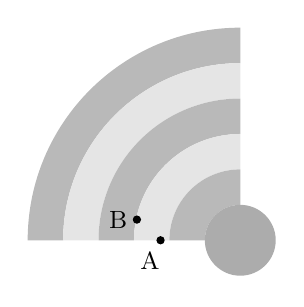
\begin{tikzpicture}[scale=0.75]

% centro dos semicírculos
\coordinate (O) at (4,0);

% semicírculos concêntricos em escala de cinza
\fill[gray!55] (O) ++(180:3.6) arc[start angle=180,end angle=90,radius=3.6] --
               ++(0,-0.6) arc[start angle=90,end angle=180,radius=3.0] -- cycle;

\fill[gray!20] (O) ++(180:3.0) arc[start angle=180,end angle=90,radius=3.0] --
               ++(0,-0.6) arc[start angle=90,end angle=180,radius=2.4] -- cycle;

\fill[gray!55] (O) ++(180:2.4) arc[start angle=180,end angle=90,radius=2.4] --
               ++(0,-0.6) arc[start angle=90,end angle=180,radius=1.8] -- cycle;

\fill[gray!20] (O) ++(180:1.8) arc[start angle=180,end angle=90,radius=1.8] --
               ++(0,-0.6) arc[start angle=90,end angle=180,radius=1.2] -- cycle;

\fill[gray!55] (O) ++(180:1.2) arc[start angle=180,end angle=90,radius=1.2] --
               ++(0,-0.6) arc[start angle=90,end angle=180,radius=0.6] -- cycle;

% disco central
\fill[gray!65] (O) circle (0.6);

% pontos A e B
\fill (2.65,0) circle (2pt);
\node[left] at (2.8,-0.35) {\small A};

\fill (2.25,0.35) circle (2pt);
\node[left] at (2.25,0.35) {\small B};

\end{tikzpicture}
\end{center}



% {
% \centering
% 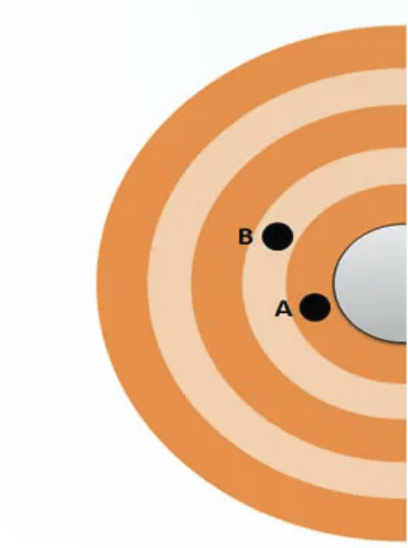
\includegraphics[width=0.15\linewidth]{imagenscinematicavetorial/ufsma_circular.png}
% \captionof{figure}{}
% \label{fig_cinvet_acentripetaufsm}
% } 

\begin{enumerate}
    \item [(a)] Em módulo, a aceleração centrípeta de A é maior do que a aceleração centrípeta de B.
    
    \item [(b)] Em módulo, as velocidades angulares de A e B são iguais.
    
    \item [(c)] A poderia acompanhar B se a velocidade angular de A fosse maior do que a de B, em módulo.
    
    \item [(d)] Se as massas dos corredores são iguais, a força centrípeta sobre B é maior do que a força centrípeta sobre A, em módulo.
    
    \item [(e)] Se A e B estivessem correndo na mesma raia, as forças centrípetas teriam módulos iguais, independentemente das massas.
\end{enumerate}


\resolucao

Avaliando o item $(a)$, sendo a aceleração centrípeta dada por $a_c = \sfrac{v^2}{R},$ e sendo as velocidades, em módulo, iguais, vemos que o indivíduo que percorrer a circunferência de menor raio -- indivíduo $A$, no caso -- terá maior aceleração centrípeta, haja vista que tais grandezas são inversamente proporcionais. \\

Logo, o item $(a)$ é o correto.

    
\end{exemplo}




\vspace{0.3cm}

\begin{exemplo}[Nível II]



Uma partícula descreve um movimento circular uniforme de raio $R$ e período $T$ em um plano horizontal. Em um certo instante, considera-se um sistema de eixos ortogonais fixos $x$ e $y$, tal que o vetor velocidade da partícula aponta exatamente na direção do eixo $y$.

Assinale a alternativa correta para as componentes da aceleração da partícula nesse instante.

\begin{enumerate}
\item [(a)] $a_x = 0$ e $a_y = \dfrac{4\pi^2 R}{T^2}$
\item [(b)] $a_x = -\dfrac{4\pi^2 R^2}{T^2}$ e $a_y = 0$
\item [(c)]$a_x = \dfrac{4\pi^2 R}{T^2}$ e $a_y = 0$
\item [(d)]$a_x = 0$ e $a_y = -\dfrac{4\pi^2 R}{T^2}$
\item [(e)]$a_x = -\dfrac{2\pi R}{T^2}$ e $a_y = \dfrac{2\pi R}{T^2}$
\end{enumerate}

\resolucao

A Figura \ref{fig_cinvet_aceleracaocentripetaexemplo02} ilustra a situação. Sendo o movimento uniforme, a aceleração será puramente centrípeta, apontando para o centro da circunferência, estando, portanto, alinhada com a direção $x.$ Logo, concluímos que $a_y=0$, de modo que descartamos as alternativas $(a)$, $(d)$ e $(e).$

{
\centering
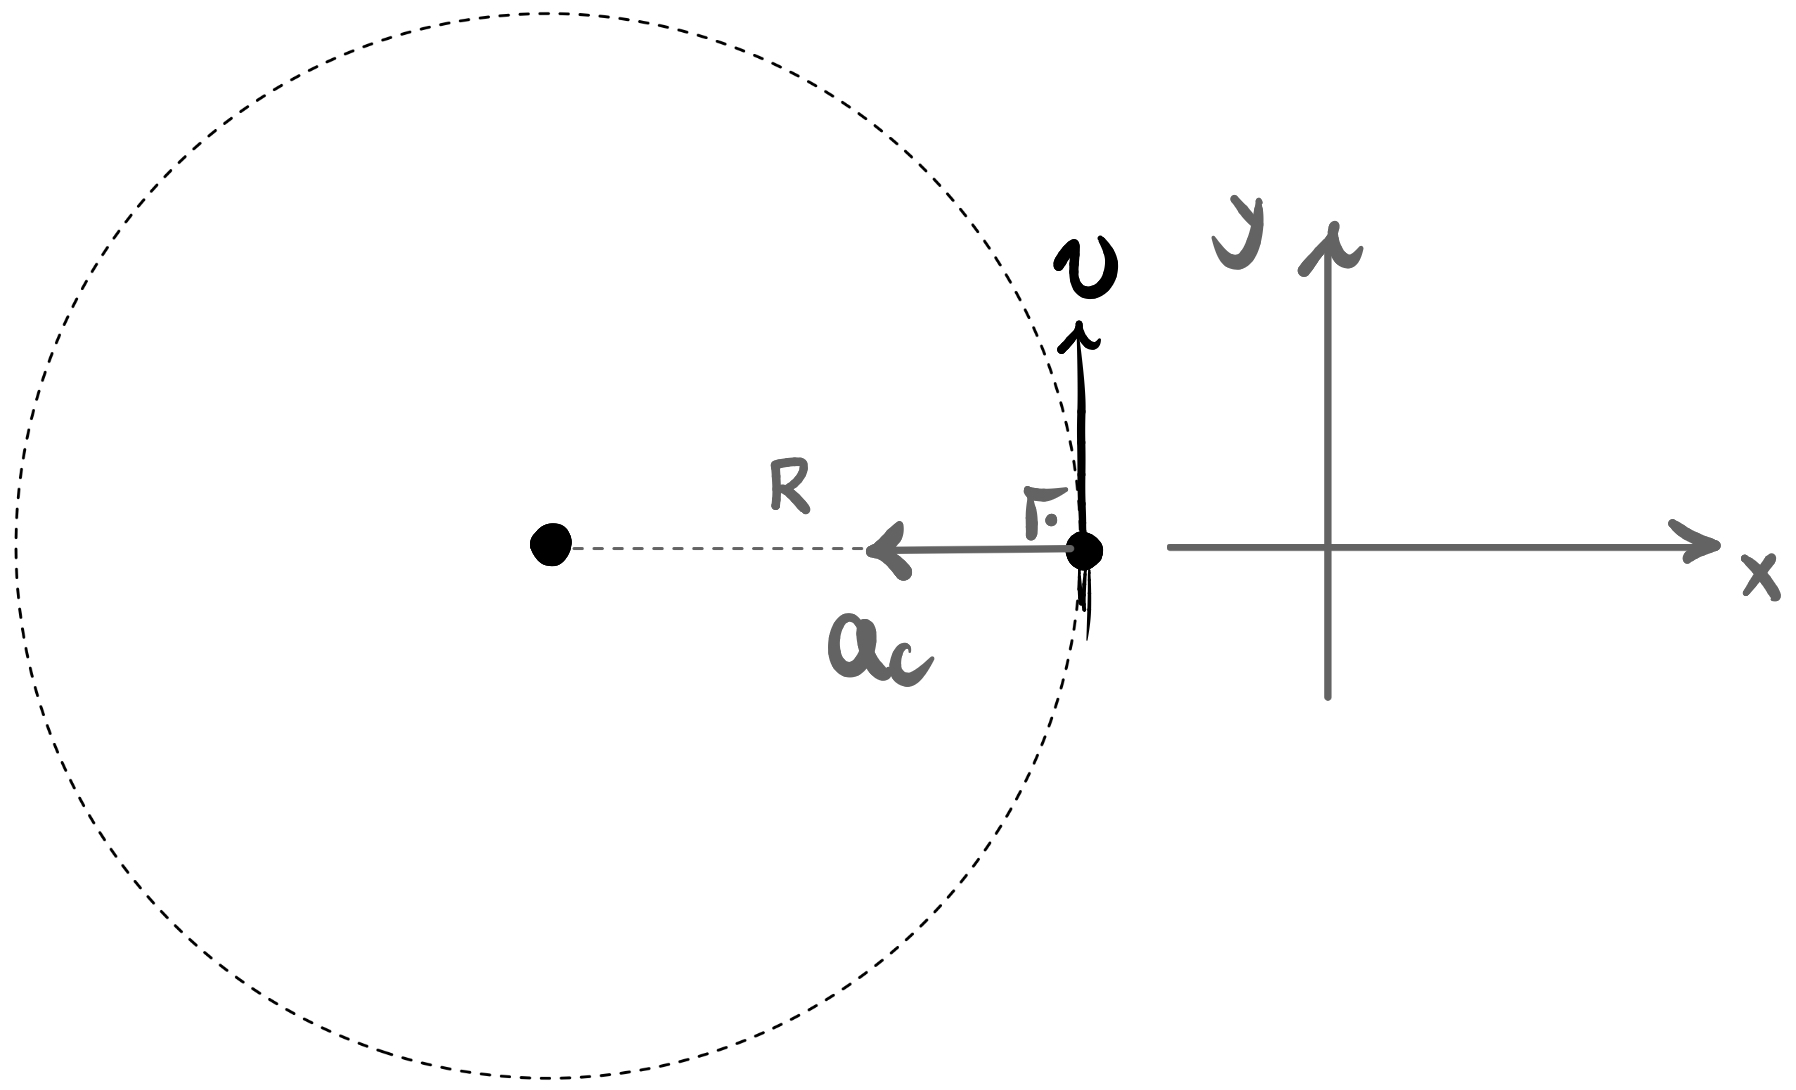
\includegraphics[width=0.4\linewidth]{imagenscinematicavetorial/aceleracaocentripetaexemplo02.jpeg}
\captionof{figure}{}
\label{fig_cinvet_aceleracaocentripetaexemplo02}
} 

A aceleração em $x$ será, portanto

$$ a_x =a_c = \dfrac{v^2}{R},$$

\noindent e, sendo o movimento uniforme, podemos usar que $v=\sfrac{d}{t}.$ Sendo $T$, o período, o tempo de uma volta, teremos que neste intervalo de tempo:

$$ v= \dfrac{d}{t} = \dfrac{2 \pi R}{T} \implies v^2 = \dfrac{4 \pi^2 R^2}{T^2},$$

\noindent e a aceleração em $x$ é, portanto,

$$ a_x = a_c = \dfrac{v^2}{R} = \dfrac{\dfrac{4 \pi^2 R^2}{T^2}}{R} \implies \boxed{a_x = \dfrac{4 \pi^2 R}{T^2},}$$

\noindent de modo que a resposta correta é a letra $(c).$
    
\end{exemplo}




\vspace{0.3cm}

\begin{exemplo}[Nível III]


Demonstre a Equação \eqref{cinvet_eq_aceleracaocentripeta} usando o conceito de aceleração escalar nas direções horizontal e vertical, computando a sobreposição desses efeitos para obter a aceleração que faz variar a direção do vetor velocidade.

\resolucao

A ideia aqui é fazer uma análise semelhante ao que fizemos no final da resolução do primeiro exemplo sobre e Equação \eqref{cinvet_eq_aceleracaovetorialmedia}, a qual convidamos que o leitor revisite para conectar melhor as ideias aqui desenvolvidas.

\vspace{0.3cm}
{
\centering
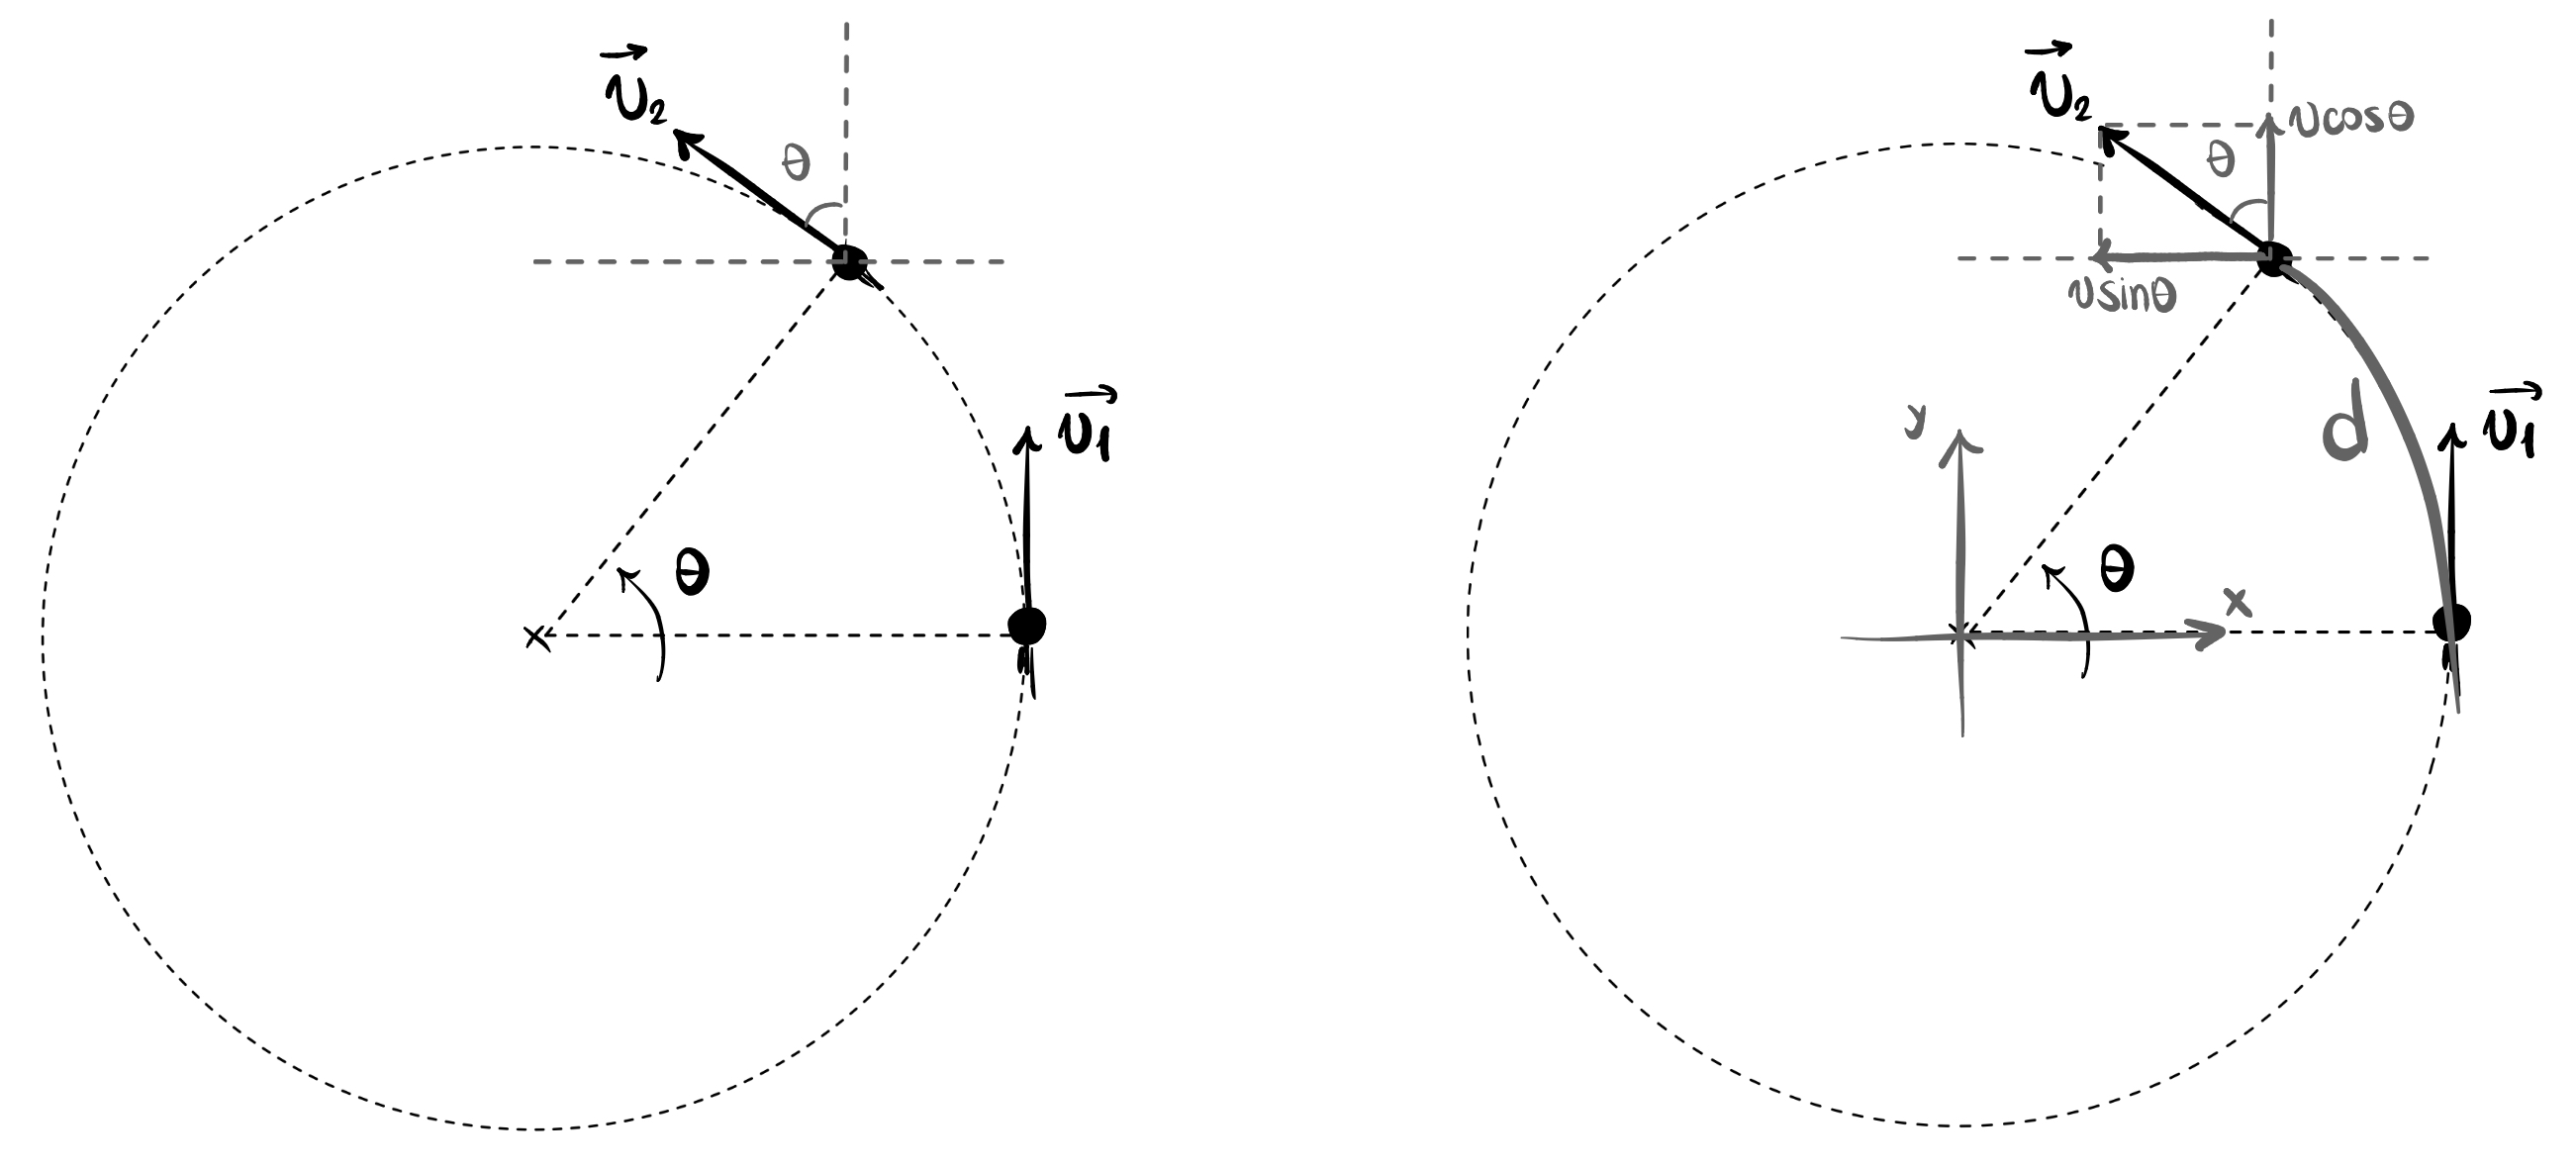
\includegraphics[width=0.8\linewidth]{imagenscinematicavetorial/aceleracaocentripetaexemplonivel3.jpeg}
\captionof{figure}{}
\label{fig_cinvet_aceleracaocentripetaexemplonivel3}
} 

Considere a primeira imagem da Figura \ref{fig_cinvet_aceleracaocentripetaexemplonivel3}, que mostra dois instantes de uma partícula que executa um MCU. Por ser um movimento uniforme, sabemos que 

$$ | \vec{v}_1| =  | \vec{v}_2| = v.$$

Entre os dois instantes $t_1$ e $t_2$, vamos considerar que atuam acelerações escalares nas duas direções $x$ e $y$, dadas por $a_x$ e $a_y,$ respectivamente. Com isso, calculamos a variação da velocidade em cada direção, o que aparece ilustrado na segunda imagem da Figura \ref{fig_cinvet_aceleracaocentripetaexemplonivel3}:

$$ \Delta v_x = -v \sin \theta - 0 \implies \boxed{ |\Delta v_x| = v \sin \theta}  \text{ e }  \Delta v_y = v \cos \theta - v \implies \boxed{ |\Delta v_y| = v  (1 - \cos \theta).} $$


Com isso, calculamos o módulo da aceleração escalar em cada direção, dado por

$$ |a_x| = \dfrac{|\Delta v_x|}{\Delta t} \implies \boxed{|a_x| = \dfrac{v \sin \theta}{\Delta t}} \quad \text{ e } \quad |a_y| = \dfrac{|\Delta v_y|}{\Delta t} \implies \boxed{|a_y| = \dfrac{v (1- \cos \theta)}{\Delta t}.}$$

Sendo as duas componentes perpendiculares, calculamos a aceleração resultante por meio do Teorema de Pitágoras:

$$ |\vec{a}|^2 = |a_x|^2 + |a_y|^2 \implies |\vec{a}|= \dfrac{v^2(\sin^2 \theta + 1 -2 \cos \theta + \cos^2 \theta)}{\Delta t},$$

\noindent que, usando a transformação do arco-metade $\sin^2 (\sfrac{\theta}{2}) = \sfrac{(1- \cos \theta)}{2},$ nos leva a

$$ |\vec{a}|= \dfrac{2v \sin (\sfrac{\theta}{2})}{\Delta t}. $$

Sendo o movimento uniforme, podemos escrever que $d=v \Delta t.$ Contudo, pela definição de radiano, temos que $\theta = \sfrac{d}{R},$ de modo que chegamos que

$$ \theta = \dfrac{v \Delta t}{R},$$

  \noindent assim, temos

  $$ |\vec{a}|= \dfrac{2v \sin (\sfrac{v \Delta t}{2R})}{\Delta t}.$$

  Por fim, como faremos a análise para um intervalo de tempo muito pequeno de modo a obter a aceleração vetorial em um instante, e não uma aceleração média entre intervalos de tempos distantes, o ângulo $\theta,$ como discutido anteriormente, será muito, muito pequeno. Usando a aproximação para ângulo pequenos $\sin \theta \approx \theta,$ que vale para $\theta$ em radianos, teremos

   $$\sin \left( \dfrac{v \Delta t}{2R} \right) \approx \dfrac{v \Delta t}{2R}, $$

   \noindent o que nos leva finalmente a

    $$ |\vec{a}|= \dfrac{2v \sin (\sfrac{v \Delta t}{2R})}{\Delta t} = \dfrac{2v}{\Delta t} \cdot \dfrac{v \Delta t}{2R} \implies \boxed{|\vec{a}|=\dfrac{v^2}{R},} $$

    \noindent como queríamos demonstrar.
  

    
\end{exemplo}




%Exemplo resolvido











\begin{secnivel}[Aceleração Tangencial]{I}{Aceleração Tangencial}
  
  \eqLdois{def}{cinvet_eq_aceleracaotangencialmedia}{a_t= a_m}

\end{secnivel}







\secgfe{De onde vem}

A bem da verdade, a Equação \eqref{cinvet_eq_aceleracaotangencialmedia} não é uma equação nova, mas sim uma reestruturação de um conceito que já conhecíamos -- o de aceleração escalar, aquela que faz variar o módulo do vetor velocidade. Tal equação está dizendo que este novo conceito que construiremos aqui -- o de aceleração tangencial, representada por $a_t$ -- coincide com o conceito de aceleração escalar que havíamos definido na Equação \eqref{mecanica_eq_aceleracaomedia}.

\vspace{0.3cm}
{
\centering
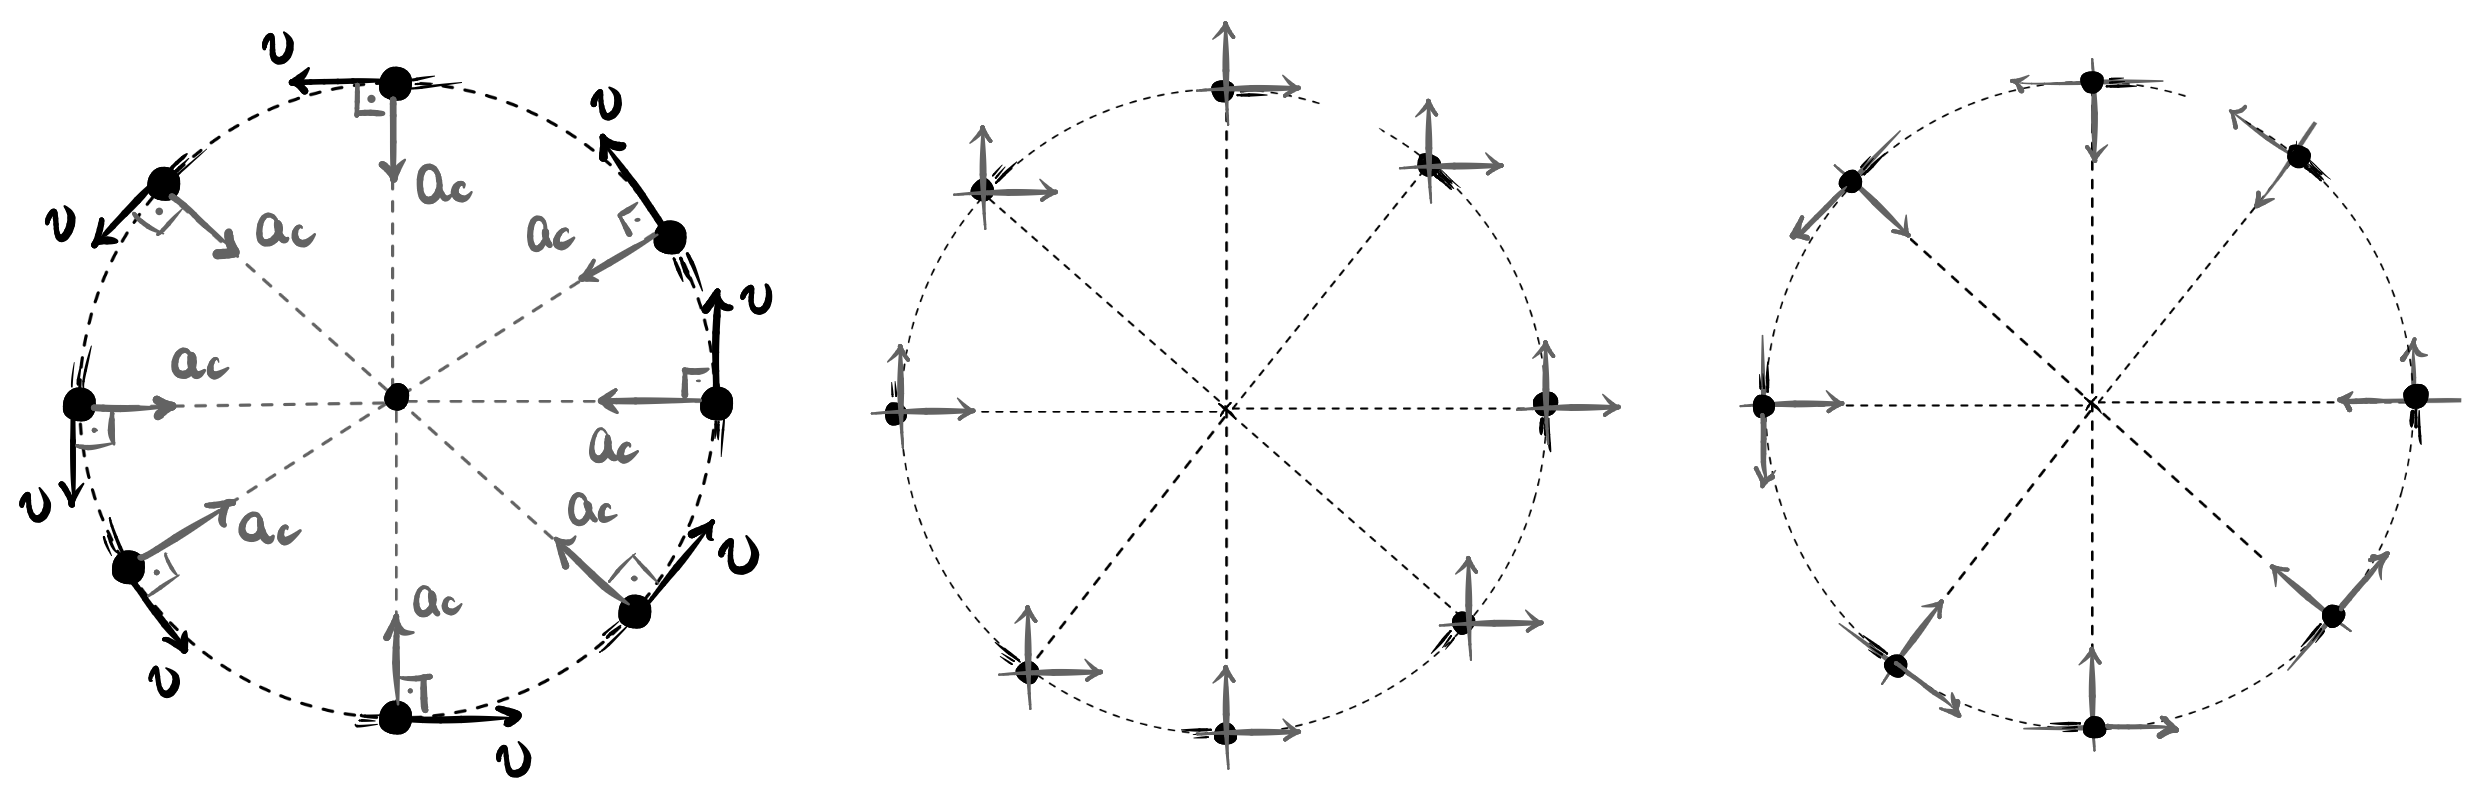
\includegraphics[width=0.9\linewidth]{imagenscinematicavetorial/aceleracaotangencial1.png}
\captionof{figure}{Os eixos mais adequados para fazer a análise das grandezas vetoriais em um movimento curvilíneo são os eixos centrípeto e tangencial.}
\label{fig_cinvet_aceleracaotangencial1}
} 
\vspace{0.3cm}

Relembre, pela Figura \ref{fig_cinvet_aceleracaotangencial1}, o que construímos até aqui: em um movimento curvilíneo a velocidade é sempre tangente à trajetória, e em tal movimento sempre há, pelo menos, um tipo de aceleração -- a aceleração responsável por variar a direção do vetor velocidade e possibilitar, portanto, que o corpo em movimento faça curva. Tal aceleração aponta sempre para o centro de curvatura, como vimos.




Note que a imagem do meio mostra uma escolha ruim de eixos ortogonais para se decompor e fazer a análise das grandezas vetoriais do problema -- um sistema de eixos fixo, vertical e horizontal. Tal sistema é ruim porque, como já vimos, todas as grandezas vetoriais estudadas até aqui em tal movimento se dão ao longo da direção tangencial e direção radial (centrípeta). Sendo assim, é muito mais conveniente adotar um sistema de eixos perpendiculares em que um deles está alinhado com a direção centrípeta e o outro com a direção tangencial.

É claro que, enquanto as direções vertical e horizontal são fixas, as direções tangencial e radial são variáveis, como mostra a terceira imagem da \ref{fig_cinvet_aceleracaotangencial1}. Desse modo, é como se nosso par de eixos ortogonais, ao invés de ser fixo, girasse junto com a partícula em movimento. Ou, caso o leitor prefira, é como se tivéssemos vários sistemas de coordenadas diferentes, um para cada ponto do movimento da partícula, sendo seus eixos sempre perpendiculares e alinhados com as direções tangente e radial à circunferência naquele ponto.

Dito isso, o que aconteceria se tivéssemos um movimento curvilíneo, em que a velocidade muda não apenas de direção, mas também tem o seu módulo alterado? Ora, se concluímos que existe um tipo de aceleração $a_c$ -- que aponta para o centro -- cujo único efeito é alterar a direção da velocidade, então é natural esperar que a aceleração $a_t$, cujo efeito será alterar o valor de tal velocidade, esteja em uma direção complementar àquela, no caso, na direção tangente à trajetória.

\vspace{0.3cm}
{
\centering
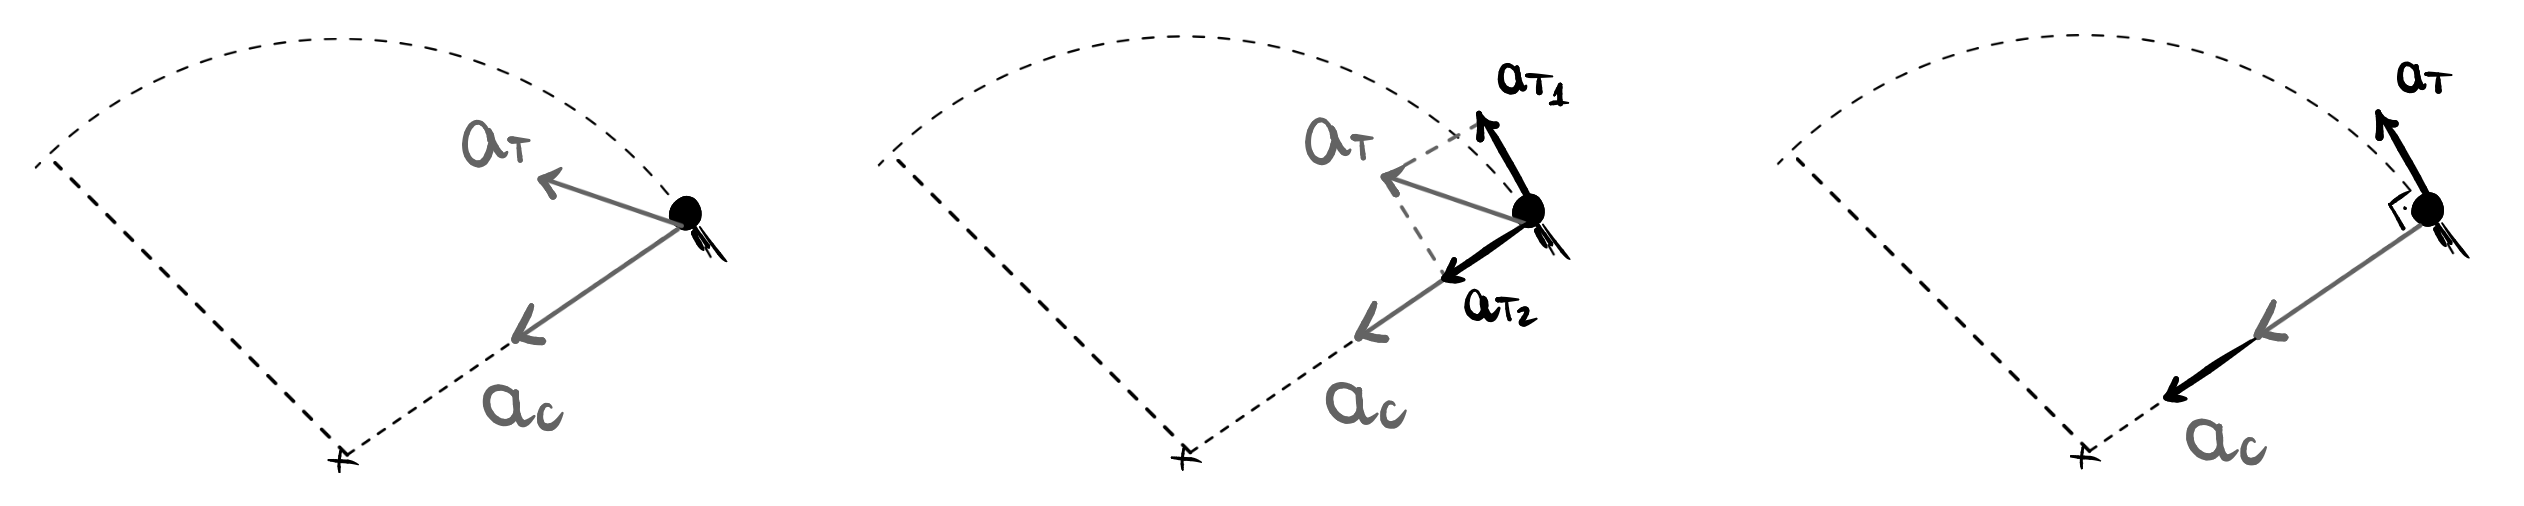
\includegraphics[width=0.9\linewidth]{imagenscinematicavetorial/aceleracaotangencial15.png}
\captionof{figure}{A aceleração responsável por alterar o módulo do vetor velocidade é paralela a tal vetor, sendo, portanto, tangente à trajetória.}
\label{fig_cinvet_aceleracaotangencial15}
} 
\vspace{0.3cm}

Para capturar bem este conceito, observe a Figura \ref{fig_cinvet_aceleracaotangencial15}. Nela, estamos assumindo que temos um movimento em que o vetor velocidade varia não apenas em direção, mas também em módulo. Já conhecemos a componente de aceleração responsável por variar a direção, é a componente $a_c,$ que aponta para o centro. Digamos que agora estamos querendo compreender como funciona a componente de aceleração $a_t$ responsável por alterar o módulo do vetor velocidade. Assim, suponha que tal componente atue sempre em uma direção oblíqua, fazendo um certo ângulo com o vetor $\vec{a}_c.$ Ora, neste caso, seria possível decompor tal vetor nas direções radial e tangencial, como mostra a segunda imagem da figura. Com isso, notaríamos que a componente de tal vetor na direção centrípeta na verdade trata-se de uma contribuição para a aceleração centrípeta, ou seja, é um tipo de aceleração que não altera o módulo do vetor velocidade. Assim sendo, a aceleração que nos restaria -- aquela que deve ser a responsável por alterar apenas o módulo do vetor velocidade -- é justamente aquela componente que se encontra integralmente na direção tangencial.




Sendo assim, concluímos aqui a essência do que diz a Equação \eqref{cinvet_eq_aceleracaotangencialmedia}: em movimentos bidimensionais que façam curvas, caso o módulo da velocidade mude, tal fato se dá devido à ação de uma componente de aceleração, chamada aceleração tangencial, que é tangente à trajetória -- e, portanto, paralela ao vetor velocidade -- e cuja ação está integralmente ligada à variação do valor da velocidade, de modo que o módulo de tal vetor pode ser computado por 

 $$ |\vec{a}_t| = \dfrac{\Delta v}{\Delta t},$$

\noindent que coincide justamente com o conceito de aceleração escalar que já conhecíamos, porém agora passando a incorporar o caráter vetorial -- a aceleração que muda o valor da velocidade deve ser sempre paralela à velocidade e, portanto, tangente à trajetória.

Observe que isso já ocorria nos casos unidimensionais antes estudados, no MUV: a nossa aceleração era sempre paralela à velocidade, podendo apontar no mesmo sentido -- casos em que o movimento seria acelerado e o valor da velocidade, portanto, aumentaria -- ou no sentido contrário -- casos em que o movimento era chamado de retardado e o valor da velocidade, portanto, diminuiria ao longo do tempo. De todo modo, a aceleração ali já respeitava essa condição de ser tangente à trajetória. Ocorre que, sendo a trajetória retilínea (movimento em uma dimensão) ser tangente a uma reta significa simplesmente que todos os vetores estão alinhados naquela mesma direção. Quando expandimos o estudo para movimentos bidimensionais é preciso estender este conceito, e é isso que o conceito de aceleração tangencial faz.


\vspace{0.3cm}
{
\centering
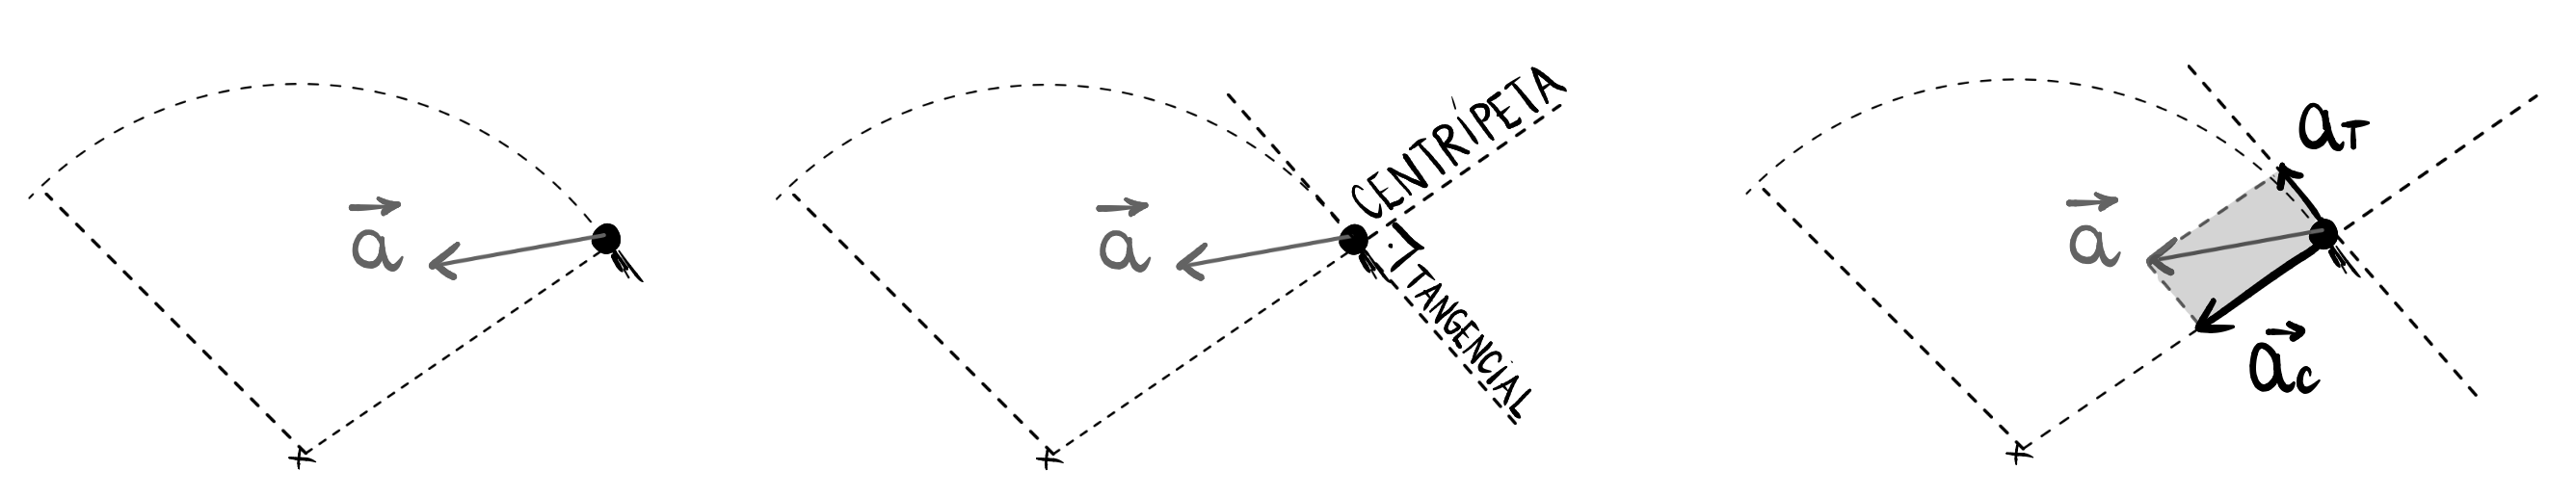
\includegraphics[width=0.9\linewidth]{imagenscinematicavetorial/aceleracaotangencial2.png}
\captionof{figure}{As componentes tangencial e centrípeta da aceleração.}
\label{fig_cinvet_aceleracaotangencial2}
} 
\vspace{0.3cm}

Por fim, observe que, de modo geral, o vetor aceleração $\vec{a}$ de uma partícula em um movimento qualquer pode apontar em uma direção qualquer, como mostra a primeira imagem da Figura \ref{fig_cinvet_aceleracaotangencial2}. Contudo, tal vetor sempre pode ser decomposto nas direções centrípeta e tangencial, resultando nas componentes $a_c$ e $a_t$ respectivamente. Cada uma dessas componentes pode ser computada e interpretada de forma separada, e o significado de cada uma delas já foi amplamente discutido e deve soar bem familiar leitor a essa altura.




Vale pontuar que, como os eixos centrípeto e radial são perpendiculares, os módulos das componentes $a_t$ e $a_c$ da aceleração $a$ podem ser relacionados pelo Teorema de Pitágoras:

$$ \boxed{a^2=a_t^2+a_c^2.}$$



\secgfe{Onde é usada}

Em problemas nos quais o \textbf{módulo da velocidade do corpo varia.} Perceba que, quando estudamos o MU e o MUV, sempre em linha reta, a aceleração que lá tratamos -- aceleração escalar -- é justamente o que, aqui, estamos chamando de aceleração tangencial: uma aceleração que atua na mesma direção do vetor velocidade e, portanto, faz variar o seu módulo, aumentando-o ou diminuindo-o.


\secgfe{Erros comuns}

O erro mais comum -- em se tratando de movimentos curvilíneos -- é quando o estudante insiste em fazer a análise das grandezas vetoriais nas direções horizontal e vertical. Como vimos na Figura \ref{fig_cinvet_aceleracaotangencial1}, as direções ideais que simplificam a análise são as direções centrípeta e radial, em cada ponto. A componente de aceleração na direção centrípeta será aquela responsável por variar a direção do vetor velocidade, e será computada pela Equação \eqref{cinvet_eq_aceleracaocentripeta}; enquanto a componente de aceleração na direção tangencial será responsável por variar o módulo do vetor velocidade, e será computada por meio da Equação \eqref{mecanica_eq_aceleracaomedia}.


\secgfe{Observações}

Vale pontuar que qualquer movimento que faça alguma curva será, certamente, um movimento acelerado: atua ali, pelo menos, a componente centrípeta da aceleração. Perceba, portanto que o movimento da primeira imagem da Figura \ref{fig_cinvet_aceleracaotangencialfinal} é acelerado, ainda que o valor da velocidade não mude.

\vspace{0.3cm}
{
\centering
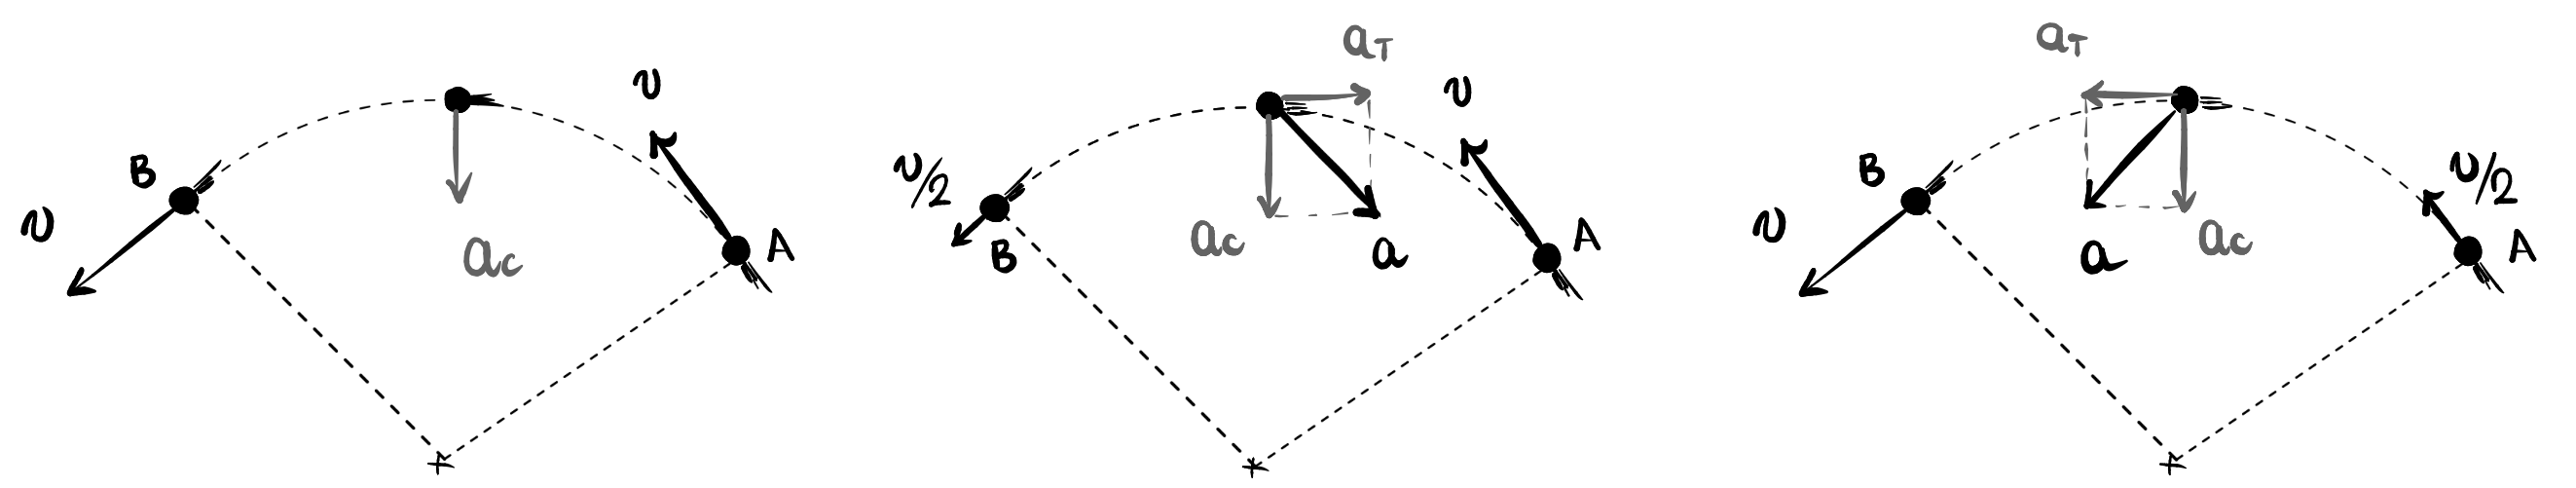
\includegraphics[width=0.9\linewidth]{imagenscinematicavetorial/aceleracaotangencialfinal.png}
\captionof{figure}{Os diferentes tipos de movimento acelerado.}
\label{fig_cinvet_aceleracaotangencialfinal}
} 
\vspace{0.3cm}

Já no movimento da imagem do meio, observamos que entre os pontos $A$ e $B$ a velocidade diminuiu. Logo, além da aceleração centrípeta, há também atuando ali a aceleração tangencial, retardando o movimento. Assim, a aceleração tangencial atua no sentido contrário ao da velocidade, contribuindo para que a aceleração resultante aponte para a direção oblíqua destacada naquele ponto intermediário do movimento.


No movimento da última imagem observamos que entre os pontos $A$ e $B$ a velocidade aumentou. Logo, além da aceleração centrípeta, há também atuando ali a aceleração tangencial, aumentando o valor da velocidade. Assim, a aceleração tangencial atua no mesmo sentido da velocidade, contribuindo para que a aceleração resultante aponte para a direção oblíqua destacada naquele ponto intermediário do movimento.




Os três movimentos da Figura \ref{fig_cinvet_aceleracaotangencialfinal} são, portanto, movimentos acelerados, uma vez que possuem algum tipo de aceleração. No primeiro o valor da velocidade é constante, então ele também pode ser chamado de movimento uniforme. No segundo o movimento seria retardado e no terceiro acelerado -- sendo essas classificações oriundas da componente tangencial da aceleração.

\vspace{0.3cm}

\begin{exemplo}[Nível I]\label{exemplo_cinematicavetorial_aceleracaotangencialex01}


Uma partícula se move em uma trajetória circular de raio $R=20.25$m. No instante $t=0$s sua velocidade é $v_0=3$ m/s, já no instante $t=2$s sua velocidade é $v=9$ m/s.

Se a taxa com que o valor da sua velocidade muda é constante, encontre, em $t=2$s

\begin{enumerate}
    \item [(a)] O módulo da aceleração tangencial da partícula.
    \item [(b)] O módulo da aceleração centrípeta da partícula.
    \item [(c)] O módulo da aceleração vetorial da partícula.
    
\end{enumerate}

\resolucao

\begin{enumerate}
   

 \item [(a)] A aceleração tangencial captura a informação de quanto varia o valor da velocidade da partícula, logo, tem-se

 $$ a_t = \dfrac{\Delta v}{\Delta t}=\dfrac{9-3}{2-0} \implies \boxed{a_t=3 \text{ m/s}^2.}$$

 \item [(b)] A aceleração centrípeta $a_c$ dependerá do valor exato da velocidade e, como este aumenta, o valor de $a_c$ será diferente em cada ponto. Em particular, para $t=2$s, teremos

  $$ a_c = \dfrac{v^2}{R} = \dfrac{9^2}{20.25} \implies \boxed{a_c= 4 \text{ m/s}^2.}$$

\item [(c)] A aceleração vetorial é o efeito resultante das acelerações calculadas anteriormente. Sendo as direções tangencial e centrípeta perpendiculares, o módulo $a$ do vetor aceleração média é obtido pela relação pitagórica

$$ a^2 = a_t^2+a_c^2 = 3^2+4^2 \implies \boxed{a= 5 \text{ m/s}^2.}$$
  \end{enumerate}
    
\end{exemplo}







\vspace{0.3cm}

\begin{exemplo}[Nível II]\label{exemplo_cinematicavetorial_aceleracaotangencialex02}

Uma partícula descreve uma trajetória circular de raio $R$. Seu movimento é tal que o módulo da aceleração total permanece constante, enquanto a velocidade escalar aumenta com o tempo. Sabendo que, em um certo instante, a velocidade da partícula é $v$, determine a aceleração tangencial $a_t$ nesse instante, em função de $v$, $R$ e do módulo constante $a$ da aceleração total.

\resolucao

Vamos primeiro tentar intuir o que deve acontecer: o valor da velocidade aumenta, logo, temos uma aceleração tangencial. Ora, mas se o valor de $v$ aumenta, então o valor $a_c$ da aceleração centrípeta também deve aumentar, uma vez que $a_c = \sfrac{v^2}{R},$ e o raio é mantido fixo.

Porém se o valor de $a_c$ aumenta, mas se o valor absoluto da aceleração vetorial é mantido constante, então a aceleração tangencial $a_t$ deve diminuir, a fim de equilibrar o aumento da componente centrípeta, mantendo a aceleração resultante constante. Vejamos isso nos cálculos. No instante em questão, a aceleração centrípeta vale

$$ a_c = \dfrac{v^2}{R},$$
\noindent e, sendo $a$ o valor do módulo da aceleração vetorial, que é mantido fixo, teremos

$$ a^2 = a_c^2 + a_t^2 \implies a_t^2 = a^2 - a_c^2=a^2 - \left(\dfrac{v^2}{R} \right)^2 \implies \boxed{a_t=\sqrt{a^2-\left(\dfrac{v^2}{R} \right)^2}.}$$

Conforme intuimos, o valor de $a_t$ decresce conforme $v$ aumenta.
    
\end{exemplo}



\vspace{0.3cm}




\begin{exemplo}[Nível II]\label{exemplo_cinematicavetorial_aceleracaotangencialex03}

Um avião se desloca em linha reta com velocidade $v_0$ e aceleração
constante $a_0$. A hélice do avião tem raio $R$. Em certo instante,
a hélice gira com velocidade angular $\omega$ e aceleração angular
$\alpha$. Determine o módulo da aceleração de um ponto localizado na
extremidade da hélice.

\resolucao

A aceleração da ponta da hélice é a soma de três parcelas:
%
\begin{equation}
    \vec{a} = \vec{a}_{\text{avião}}
            + \vec{a}_{\text{tangencial}}
            + \vec{a}_{\text{centrípeta}}.
\end{equation}
%
Temos:
%
\begin{align}
    a_{\text{avião}}     &= a_0,    \nonumber  \\
    a_{\text{tangencial}}&= R\alpha, \nonumber \\
    a_{\text{centrípeta}}&= R\omega^2. \nonumber
\end{align}
%
Como essas três acelerações são perpendiculares entre si, o módulo é dado pelo Teorema de Pitágoras:
%
\begin{equation}
    a = \sqrt{a_0^2 + (R\alpha)^2 + (R\omega^2)^2}.
    \nonumber
\end{equation}
%
Portanto:
%
\begin{equation}
    \boxed{a = \sqrt{a_0^2 + R^2\alpha^2 + R^2\omega^4}.}
    \nonumber
\end{equation}

Vale a pena pausar e visualizar o caminho que esse ponto traça no
espaço. Escolhendo o eixo $x$ ao longo da direção de voo, a posição
da ponta da hélice pode ser escrita como
%


\begin{equation}
\begin{cases}
    x(t) =  \left(v_0 t + \tfrac{1}{2}a_0 t^2\right) \\[6pt] 
    y(t) = R\cos\!\left(\omega t + \tfrac{1}{2}\alpha t^2\right) \\[6pt] 
    z(t) = R\sin\!\left(\omega t + \tfrac{1}{2}\alpha t^2\right)
\end{cases}
    \nonumber
\end{equation}

%
As componentes $y$ e $z$ descrevem um movimento circular de raio
constante $R$ no plano perpendicular ao voo, enquanto a componente
$x$ avança continuamente. O resultado é uma \textit{hélice espacial}
— a mesma forma de um parafuso ou de uma mola esticada.

No caso mais simples, em que $a_0 = 0$ e $\alpha = 0$ (avião em
velocidade constante, hélice em rotação uniforme), a hélice é
\emph{uniforme}: cada volta ocupa exatamente o mesmo espaço ao longo
do eixo $x$, e as três acelerações se reduzem a apenas uma — a
centrípeta $R\omega^2$, apontando para o eixo da hélice.

Quando $a_0 \neq 0$ ou $\alpha \neq 0$, a hélice deixa de ser
uniforme. A aceleração $a_0$ altera o espaçamento entre voltas
consecutivas (o passo da hélice cresce se o avião acelera), enquanto
$\alpha$ altera a velocidade com que o ponto percorre cada volta,
``comprimindo'' ou ``expandindo'' as espiras ao longo do tempo. É
precisamente essa não-uniformidade que dá origem às componentes
tangencial ($R\alpha$) e linear ($a_0$) na expressão do módulo da
aceleração.


\end{exemplo}

\vspace{0.3cm}















\chapter{Movimento Circular}




\begin{secnivel}[Frequência e Período]{I}{Frequência e Período}
  
  \eqLdois{def}{cinvet_eq_freqeperiodo}{f = \dfrac{1}{T}}

\end{secnivel}







\secgfe{De onde vem}

Existem duas grandezas que aparecem na Equação \eqref{cinvet_eq_freqeperiodo}, o período $T$ e a frequência $f.$ Essas duas grandezas se referem a movimentos periódicos, ou seja, movimentos que se repetem, como um pêndulo que oscila de um lado para o outro, um carro de fórmula 1 que dá repetidas voltas em uma mesma pista ou uma partícula em movimento circular.

O período $T$ é definido como sendo o tempo necessário para que a partícula complete um ciclo completo. No caso de um pêndulo, seria o tempo necessário para sair de um extremo, ir até o outro e depois retornar ao ponto inicial. No caso de uma partícula em movimento circular seria o tempo necessário para dar uma volta. Logo, se o movimento circular for uniforme, sendo $R$ o raio da circunferência, poderíamos escrever que 

$$ v = \dfrac{d}{t} = \dfrac{2 \pi R}{T},$$

\noindent que é uma equação que evidencia o significado de $T:$ é o tempo necessário para que se percorra uma volta completa, que no caso da circunferência, vem a ser a distância $2 \pi R.$

Já a frequência $f$ é definida como o inverso do período, e é isso que aparece na Equação \eqref{cinvet_eq_freqeperiodo}. Se o período, portanto, computa o tempo por volta, o inverso disso seria quantas voltas se dá por tempo -- essa é a frequência $f$.

Considere, por exemplo, um corpo em movimento circular uniforme, executando 12 voltas a cada minuto. Isso seria a frequência $f$. O tempo para se executar uma única volta pode ser obtido por regra de três, ou pela aplicação direta da Equação \eqref{cinvet_eq_freqeperiodo}:

$$ T = \dfrac{1}{f}=\dfrac{1}{\sfrac{12 \text{ voltas}}{1 \text{ min}}} = \dfrac{1 \text{ min}}{12 \text{ voltas}} = \dfrac{60 \text{ segundos}}{12 \text{ voltas}} = \boxed{ \dfrac{5 \text{ s}}{1\text{ volta}},}$$

\noindent ou seja, o período -- tempo de uma volta -- é de 5 segundos.

As unidades de medida foram carregadas ao longo do cálculo por dois motivos: primeiro para evidenciar de forma explícita o significado do resultado computado -- o tempo por ciclo ou volta. Segundo para que o leitor perceba que, muitas vezes, será conveniente fazer algumas conversões de unidades, tal como trocar minutos por segundos, como fizemos acima.

\secgfe{Onde é usada}

Os conceitos de frequência e período e, consequentemente, a Equação \eqref{cinvet_eq_freqeperiodo}, são amplamente utilizados no estudo de movimentos periódicos, como movimentos oscilatórios (MHS), movimentos ondulatórios ou movimentos circulares.


%\secgfe{Erros comuns}





\secgfe{Observações}

Cabe aqui uma observação sobre unidades de medida. A unidade de medida no Sistema Internacional (S.I.) para tempo é o segundo, de modo que a unidade de medida no S.I. seria $\sfrac{1}{s},$ a que dá-se o nome de Hertz (Hz). Assim, uma frequência de $1.200$Hz significa que a partícula completa 1200 ciclos a cada segundo. Uma frequência de $5.000$Hz significam $5.000$ ciclos realizados a cada segundo.

É comum também que se apareçam frequências em r.p.m (rotações por minuto), que podem facilmente ser convertida para Hertz pela conversão direta de minutos em segundos. Como exemplo, considere uma frequência de 120 voltas por minuto, isto é, 120 r.p.m:

$$  \dfrac{120\text{ rotações}}{1 \text{ minuto}} = \dfrac{120\text{ rotações}}{60 \text{ segundos}} = \dfrac{2\text{ rotações}}{1 \text{ segundo}} = 2 \text{ Hz.}$$

Raciocínio análogo se aplica à unidade de medida r.p.h (rotações por hora). Neste caso, usaremos o fato de uma hora equivale a $3600$ segundos, de modo que a frequência, por exemplo, de 7200 r.p.h é igual a

$$ \dfrac{7200\text{ rotações}}{1 \text{ hora}} =  \dfrac{7200\text{ rotações}}{3600 \text{ segundos}} = \dfrac{2 \text{ rotações}}{1 \text{ seg}} = 2 \text{ Hz,} $$

\noindent ou seja, a frequência de 7200 r.p.h é igual à frequência de 120 r.p.m.

\vspace{0.3cm}


\begin{exemplo}[Nível I]\label{exemplo_cinvet_periodofrequenciaex01}

Considere uma partícula que executa um MCU com frequência igual a $3 \text{s}^{-1}$ , em uma circunferência cujo raio é $R=2$m. Calcule a velocidade da partícula.

\resolucao

Sendo o movimento uniforme, temos que

$$ v=\dfrac{d}{t}=\dfrac{2 \pi R}{T} = 2 \pi R \cdot \dfrac{1}{T} = 2 \pi R f.$$

\noindent Perceba que usamos o fato de que, em um período $T$, a partícula completa uma volta, ou seja, percorre a circunferência inteira. Posteriormente usamos que a frequência é o inverso do período, chegando na equação final que permite computar diretamente a velocidade a partir dos parâmetros fornecidos:

$$ v = 2 \pi R f \approx 2 \cdot 3 \cdot 2 \text{m} \cdot 3 \text{s}^{-1} = 36 \text{ m/s}.$$

\noindent Note que a frequência fornecida, na unidade inverso de segundo, isto é $\sfrac{1}{s}=s^{-1}$, é justamente o Hertz.

\end{exemplo}





\begin{secnivel}[Velocidade Angular Média]{I}{Velocidade Angular Média}
  
  \eqLdois{def}{cinvet_eq_velangular}{\omega_m = \dfrac{\Delta \theta}{\Delta t}}

\end{secnivel}










\secgfe{De onde vem}

Considere uma partícula que descreve um movimento cuja trajetória é circular. Com tudo que já vimos até aqui de Cinemática -- posição, velocidade média, aceleração média, etc é possível descrever, de forma precisa e completa, quaisquer tipos de movimentos -- em particular, movimentos circulares.

Entretanto, para tais movimentos, pode ser muito mais conveniente descrevê-los a partir de grandezas angulares do que lineares. Isto é, ao invés de descrever o deslocamento da partícula por meio do comprimento linear $\Delta s$ da sua trajetória -- que chamaremos aqui de deslocamento linear -- podemos fazê-lo por meio do seu deslocamento angular $\Delta \theta$.

\vspace{0.3cm}
{
\centering
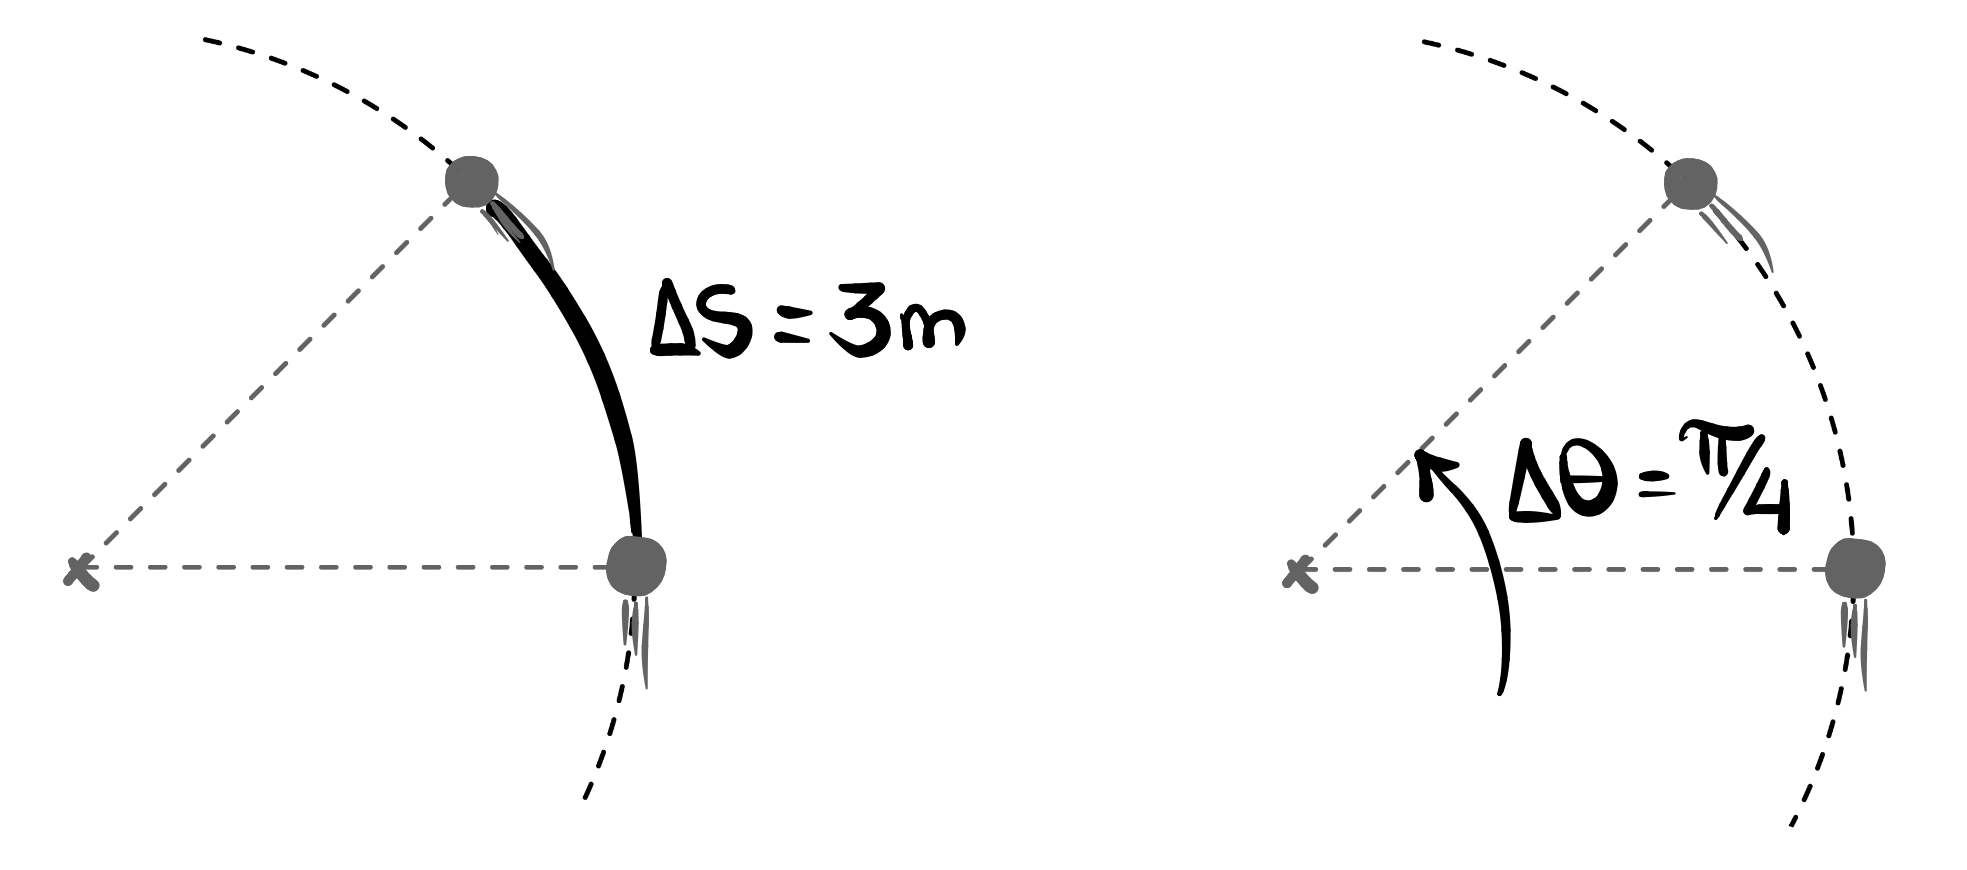
\includegraphics[width=0.6\linewidth]{imagenscinematicavetorial/deslocamentoangular.png}
\captionof{figure}{O deslocamento linear e angular.}
\label{fig_cinvet_deslocamentoangular}
} 
\vspace{0.3cm}


Dada uma circunferência, veja que existem duas formas equivalentes de se expressar o deslocamento de um corpo. No caso da Figura \ref{fig_cinvet_deslocamentoangular}, dizer que o corpo, em um certo intervalo de tempo, se deslocou 3 metros; ou dizer que ele se deslocou 45 graus, ou seja, $\sfrac{\pi}{4}$ radianos, são informações equivalentes. Das duas formas conseguimos, dada uma posição inicial, descobrir onde o corpo estará no próximo instante de tempo, ou seja, nos permitem fazer uma descrição cinemática do movimento do corpo.

Sendo assim, podemos criar uma grandeza angular análoga à velocidade média definida na Equação \eqref{mecanica_eq_velocidademedia}. Ora, se lá definimos a velocidade linear\footnote{Para diferenciar as grandezas, o que já conhecíamos como velocidade, será aqui chamada de velocidade linear. Trata-se da mesma grandeza até então conhecida por nós -- é uma acréscimo de vocabulário apenas para certificar de que vamos conseguir diferenciar com clareza $v$ de $\omega$, isto é, a velocidade linear da velocidade angular.} $v$ como sendo a razão entre o deslocamento linear $\Delta s$ pelo intervalo de tempo; é natural que se defina a velocidade angular $\omega$ como sendo a razão entre o deslocamento angular $\Delta \theta$ e o intervalo de tempo, que é justamente o que aparece na Equação \eqref{cinvet_eq_velangular}.

Perceba que, enquanto a velocidade linear $v$ mede o quão rápido se percorre uma distância, ou seja, quantos metros se percorre por segundo; a velocidade angular $\omega$ mede o quão rápido se percorre um ângulo, ou seja, quantos radianos se gira por segundo, por exemplo.



\secgfe{Onde é usada}

Em quaisquer problemas que envolvam movimentos periódicos, em particular, para movimentos circulares.


\secgfe{Erros comuns}

O erro mais comum aqui é o estudante querer usar os ângulos em graus e não em radianos. Isso, eventualmente, pode levá-lo a alguns erros, que estarão relacionados à natureza geométrica da definição de radiano. Na seção em que apresentaremos a Equação \eqref{cinvet_eq_velangularelinear} vamos discutir em detalhes este fato e ficará claro por qual razão é mais natural usar radianos e não graus. Por hora, fica a ressalva ao leitor: o ideal que todos os ângulos, em equações físicas, sejam calculados e inseridos em radianos.

Desse modo, a unidade padrão no S.I. para velocidade angular é o rad/s.


\secgfe{Observações}

O contexto mais comum em que aplicaremos a Equação \eqref{cinvet_eq_velangular} será o de movimentos circulares, em particular, o movimento circular uniforme (MCU). Em tal contexto, a velocidade angular $\omega$, por ser constante, será igual à velocidade angular média $\omega_m$ em qualquer intervalo de tempo, ou seja

$$ \omega_m = \omega = \dfrac{\Delta \theta}{\Delta t}.$$

No intervalo de tempo de um período $T$, o ângulo total girado será o de uma volta, isto é, $\Delta \theta = 2\pi$ rad, logo, teremos

$$ \omega =  \dfrac{\Delta \theta}{\Delta t} = \dfrac{2 \pi}{T} \implies \boxed{\omega =  \dfrac{2 \pi}{T} .}$$

Além disso, sendo a frequência o inverso do período, poderíamos escrever a equação acima como

$$ \omega = \dfrac{2 \pi}{T} = 2 \pi \cdot \dfrac{1}{T} = 2 \pi f \implies \boxed{\omega = 2 \pi f.}$$

As duas equações destacadas acima são apenas uma pequena variação da Equação \eqref{cinvet_eq_velangular}, \textbf{válidas exclusivamente para o MCU.} É comum que as usemos para resolver certos problemas, mas é importante que o leitor perceba que tais equações não são exatamente novas e sequer precisam ser memorizadas. São apenas um caso particular da própria definição de velocidade angular, aplicada ao MCU fixando o intervalo de tempo como sendo o de uma volta.

\vspace{0.3cm}


\begin{exemplo}[Nível I]\label{exemplo_cinvet_velocidadeangularex01}

Um ventilador realiza 120 rotações por minuto. Sendo a dimensão da sua pá de 15 cm, calcule a velocidade linear da extremidade da pá e sua velocidade angular.

\resolucao

A frequência é de 

$$\dfrac{120 \text{ rot.}}{1\text{ min}} = \dfrac{120 \text{ rot.}}{60 \text{ s}} = 2 s^{-1}.$$ 


Assim, a velocidade angular $\omega$ é

$$ \omega = \dfrac{\Delta \theta}{\Delta t} = \dfrac{2 \pi}{T} = 2 \pi \cdot \dfrac{1}{T} = 2 \pi f,$$

\noindent em que usamos que o ângulo total girado em um período é o de uma volta completa, isto é, $2 \pi $ rad, e que a frequência é o inverso do período. Substituindo os valores teremos

$$ \omega =2 \pi f =4 \pi\text{ rad/s} \approx 12 \text{ rad/s}.  $$

Já a velocidade linear $v$ é

$$ v = \dfrac{d}{t} = \dfrac{2 \pi R}{T} = 2 \pi R \cdot \dfrac{1}{T} = 2 \pi R f,$$

\noindent que, substituindo, fornece:

$$ v = 2 \pi R f = 2 \pi \cdot 0.15 \text{m} \cdot 2 s^{-1} = 0.6 \pi \text{ m/s} \approx 1.9 \text{ m/s}.$$

\end{exemplo}



\vspace{0.3cm}


\begin{exemplo}[Nível II]\label{exemplo_cinvet_velocidadeangularex02}

Um corpo descreve um movimento circular uniforme de raio $R$. Sua velocidade linear é $v$. Determine o tempo necessário para que ele descreva um ângulo de $5$ radianos.


\resolucao

Usando a definição de velocidade angular, temos

$$ \omega = \dfrac{\Delta \theta}{\Delta t} = \dfrac{5}{\Delta t} \implies \Delta t = \dfrac{5}{\omega}.$$

Sendo assim, o problema consiste em encontrar a velocidade angular $\omega$ da partícula.

Sabemos sua velocidade linear $v$ e o raio $R$ da circunferência. Com isso, temos

$$ v = \dfrac{d}{t}=\dfrac{2 \pi R}{T} = \underbrace{\dfrac{2 \pi}{T}}_{\substack{\text{velocidade}\\\text{angular}}}\cdot R = \omega R \implies \omega = \dfrac{v}{R}.$$

Tal relação é tão importante que merece uma discussão à parte -- assunto para a próxima seção. Logo, tendo $\omega$ em termos dos parâmetros fornecidos, teremos o tempo pedido:

$$ \Delta t = \dfrac{5}{\omega} = \dfrac{5}{\sfrac{v}{R}} \implies \boxed{\Delta t = \dfrac{5R}{v} .} $$





\end{exemplo}





\begin{secnivel}[Relação entre $v$ e $\omega$.]{I}{Relação entre velocidade linear e angular}
  
  \eqLdois{dem}{cinvet_eq_velangularelinear}{v = \omega r}

\end{secnivel}






\secgfe{De onde vem}

A Equação \eqref{cinvet_eq_velangularelinear} mostra como podemos converter uma grandeza angular, como a velocidade angular $\omega$, no seu análogo linear, isto é, na velocidade linear $v:$ basta usar o raio $r$ de curvatura como fator de conversão.

Isso vem de um fato geométrico, relativo ao modo como definimos o radiano. Antes, lembremos como é definido um ângulo medido em graus: divida uma circunferência em 360 partes iguais. O ângulo de 1 grau é igual ao ângulo de abertura de uma dessas partes.

É por isso que uma volta completa tem $360^\circ$: por definição. Poderíamos muito bem ter escolhido dividir a circunferência em 120 partes iguais -- ou até mesmo em 100 partes iguais, dado o fato de que usamos um sistema decimal e tudo funciona de dez em dez. O fato de que o grau é definido como sendo uma parte em 360 da circunferência é herança dos babilônios, que usavam um sistema sexagesimal (base 60), mas não vamos entrar em grandes detalhes nisso. 


\vspace{0.3cm}
{
\centering
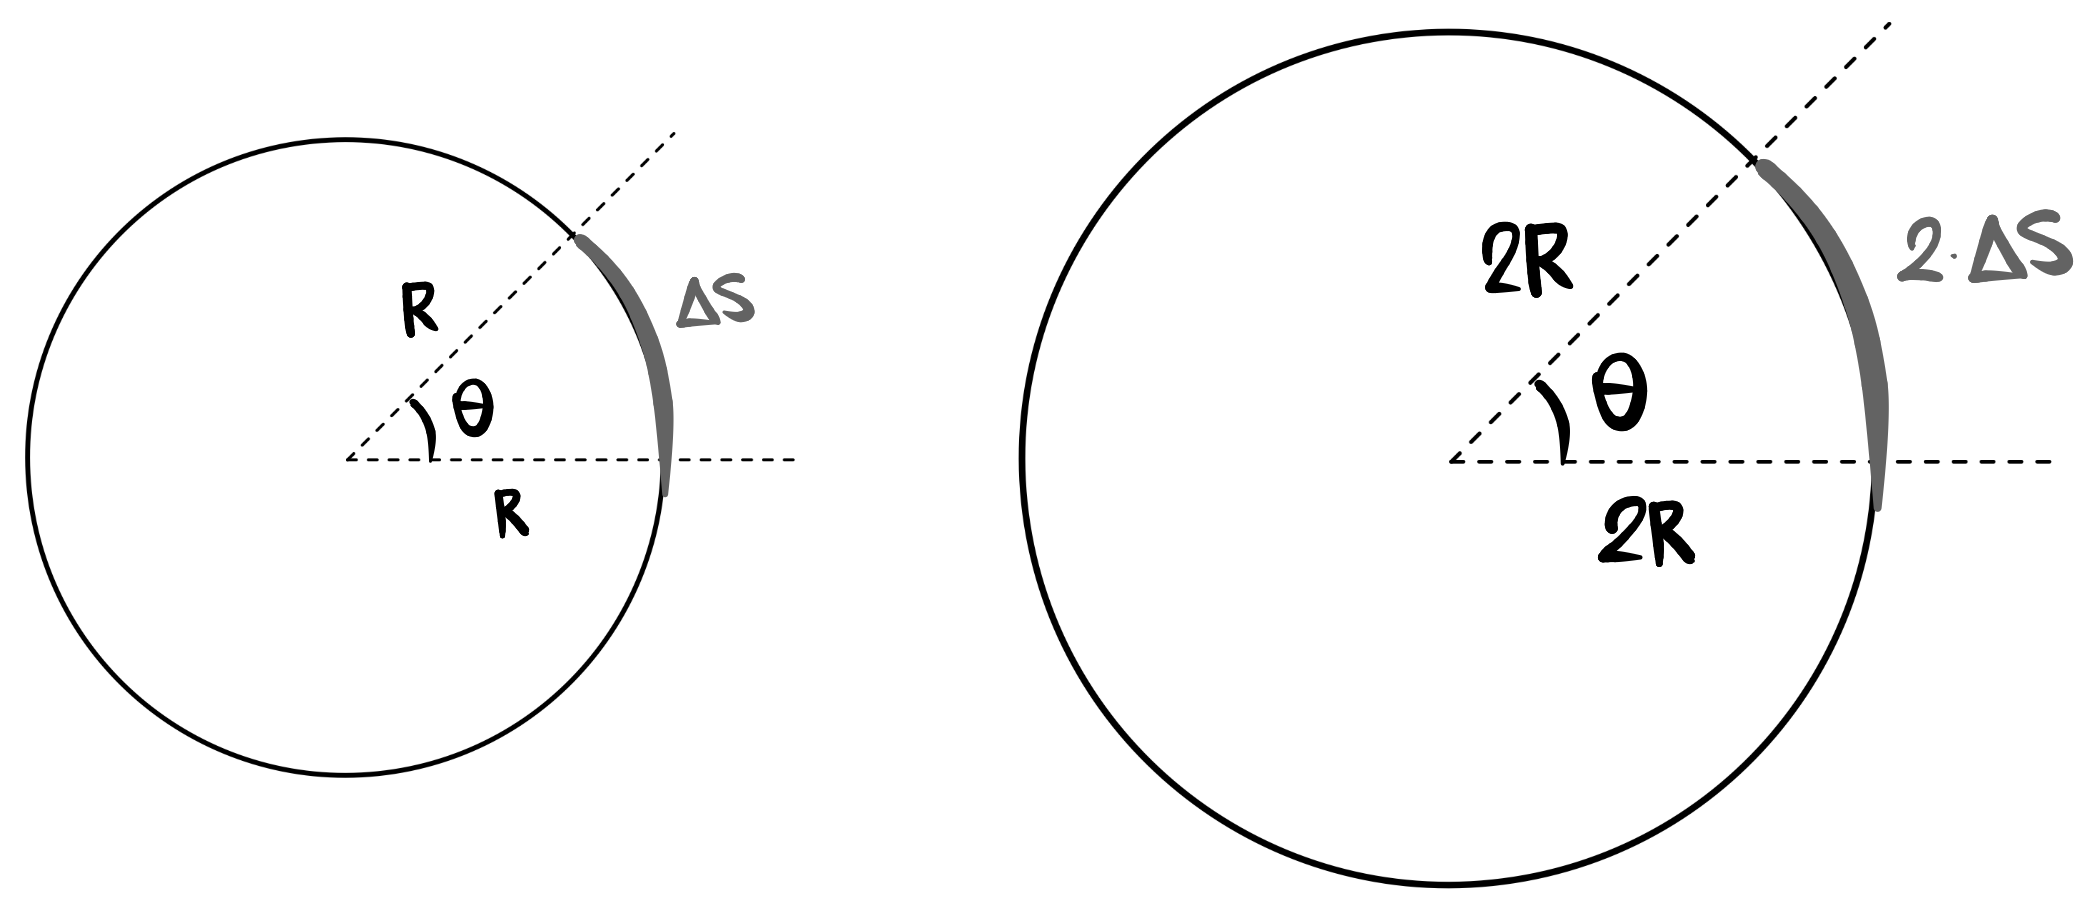
\includegraphics[width=0.5\linewidth]{imagenscinematicavetorial/definicaoradiano1.png}
\captionof{figure}{A unidade de medida natural para ângulos consiste em usar o próprio raio da circunferência como unidade de medida.}
\label{fig_cinvet_defradiano1}
} 

\vspace{0.3cm}

O fato é que existe uma outra forma de se definir a medida de ângulos -- uma forma bem menos artificial, diga-se de passagem. Tal maneira consiste em se usar o próprio raio da circunferência como unidade de medida: um ângulo $\theta$ em radianos é definido como sendo a razão entre o comprimento $\Delta s$ do arco de circunferência que ele subentende e o raio da circunferência $R$:

$$ \theta := \dfrac{\Delta s}{R}.$$





A Figura \ref{fig_cinvet_defradiano1} ilustra o fato de que, ao definir o ângulo dessa forma, a medida do ângulo independe da circunferência que usamos para medi-lo. Isso porque, avaliando a mesma abertura angular em uma circunferência que tenha o dobro do raio, vemos que, por ter o dobro do raio, o arco de circunferência referente à mesma abertura angular terá o dobro de comprimento, de modo que a razão entre essas duas grandezas será a mesma:

$$ \theta = \dfrac{\Delta s}{R} = \dfrac{2 \Delta s}{2R},$$


\noindent ou seja, independente da circunferência que se use, medindo o ângulo dessa forma seremos sempre levados ao mesmo valor.


Essa é, portanto, a forma mais natural de se medir o ângulo: usando como régua de medida o próprio raio da circunferência -- e já vimos que isso nos leva a uma medida angular que independe do raio da circunferência, ou seja, trata-se de uma medida, de certo modo, absoluta (e não relativa a uma circunferência específica). Note que tal forma de medir nos leva a um número adimensional: a razão entre dois comprimentos, $\Delta s$ e $R,$ respectivamente. 

Assim, o ângulo de uma unidade nesse sistema significaria uma abertura angular tal que o comprimento de arco na circunferência referente a tal abertura fosse de exatamente um raio. Um ângulo de duas unidades, por sua vez, representaria uma abertura angular tal que o comprimento de arco na circunferência referente a tal abertura fosse de exatamente dois raios. A Figura \ref{fig_cinvet_defradiano2} ilustra essas situações, mostrando que, para um ângulo de 3 unidades, isto é, uma abertura angular que enxerga um arco de três raios de comprimento, teremos varrido quase meia circunferência.


\vspace{0.3cm}
{
\centering
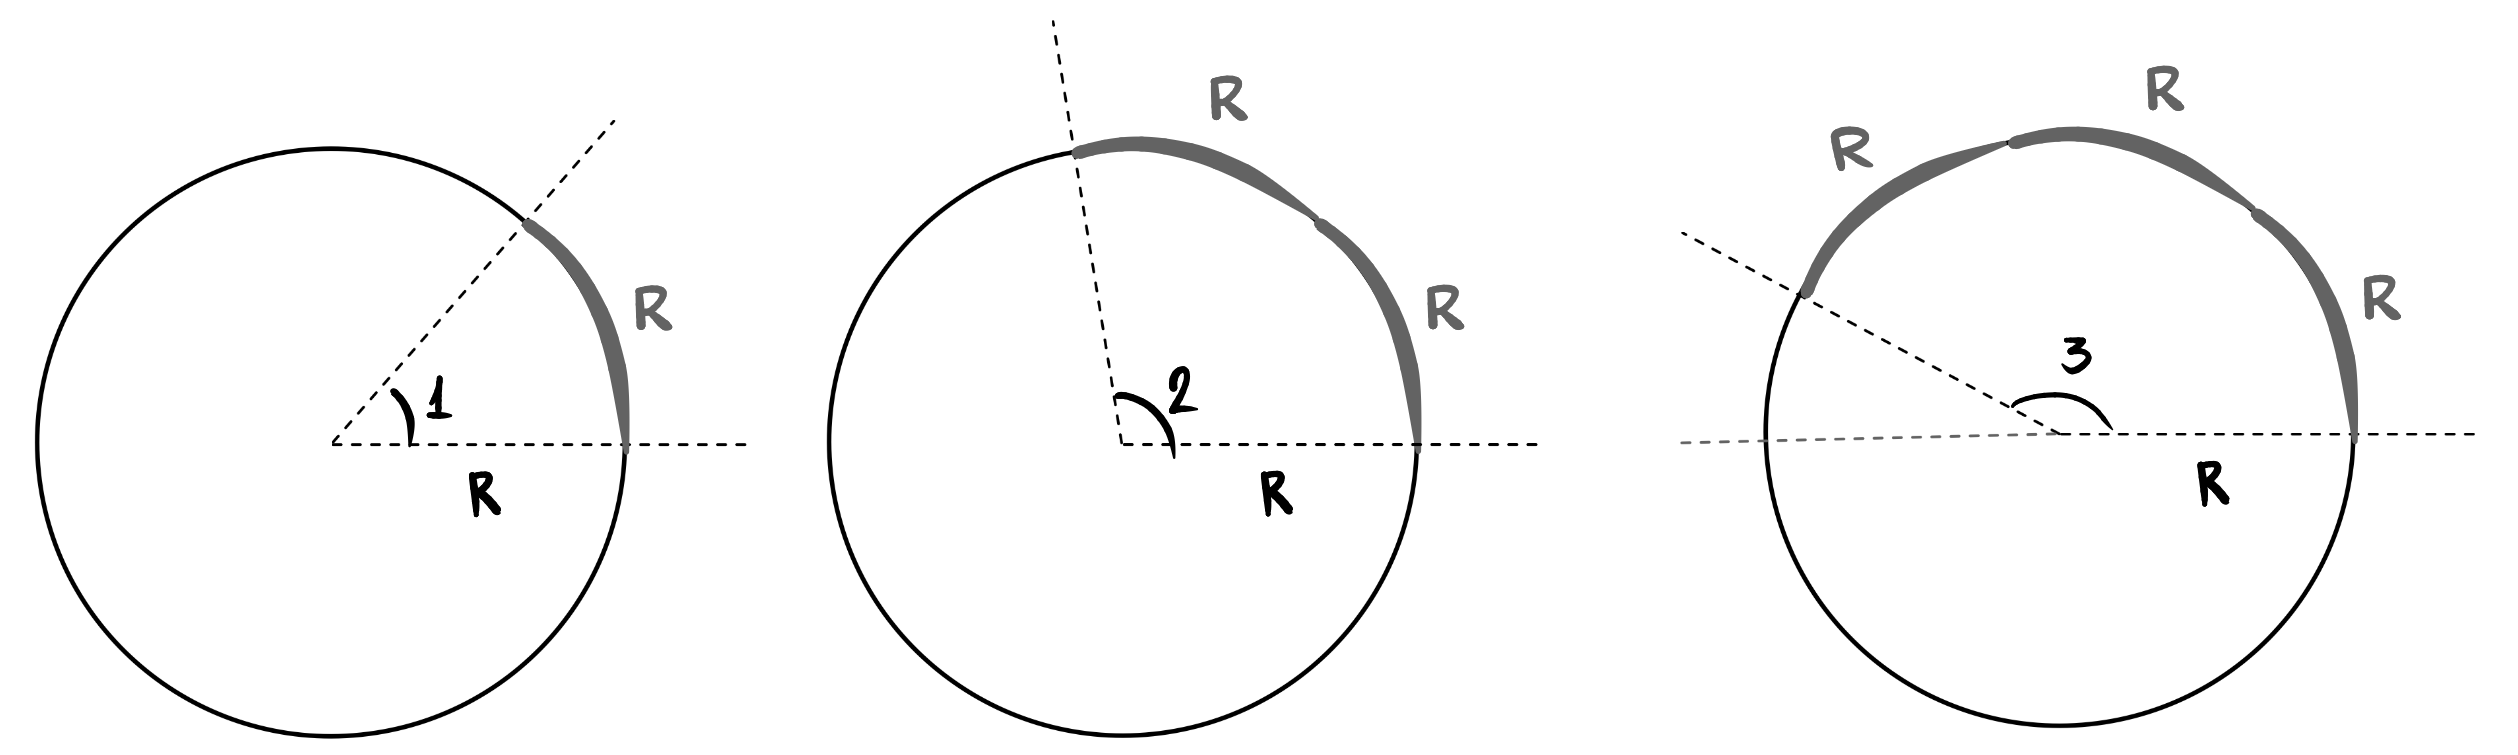
\includegraphics[width=0.8\linewidth]{imagenscinematicavetorial/definicaoradiano2.png}
\captionof{figure}{Alguns ângulos em radianos.}
\label{fig_cinvet_defradiano2}
} 

\vspace{0.3cm}
Para varrer exatamente meia circunferência precisaríamos na verdade de um ângulo de medida $\pi \approx 3,14$, ou seja, um ângulo que enxerga um arco de circunferência de 3,14 raios de comprimento. É fácil notar isso, uma vez que sabemos o comprimento de uma circunferência completa, de modo que o ângulo de uma volta completa é de

$$ \theta = \dfrac{\Delta s}{R} = \dfrac{2 \pi R}{R} = 2 \pi,$$

\noindent e, portanto, o ângulo de meia volta é de $\pi \approx 3,14$.


Para não deixar ambiguidade em relação a essa forma de medir ângulos, damos a ela um nome: radiano. Isso é só para que não haja confusão quando alguém te disser algo como \textit{considere um ângulo de medida 2...}

Ora, 2 o quê? 2 graus? Ou seria um ângulo tal que ele enxerga um arco de circunferência de comprimento igual a 2 raios? Por ser adimensional, essa nova unidade de medida pode gerar esse tipo de dúvida, de modo que damos a ela o nome de radiano: a abertura angular tal que o comprimento de arco na circunferência referente a tal abertura é de exatamente dois raios tem medida de 2 radianos. 

É importante notar, porém, que para o ângulo de $2$ rad, o termo rad não é exatamente uma unidade de medida -- o ângulo medido dessa forma é, na verdade, adimensional, por ser uma razão entre dois comprimentos. Assim, o rad é apenas um nome que conectamos com o número para eliminar algum tipo de dúvida em relação a qual é a forma que está sendo usada para medir ângulos (alguns autores chamam isso de \emph{unidade auxiliar}.)

Talvez o leitor pense que todo esse devaneio -- puramente matemático -- a respeito do que é um radiano não tenha nada a ver com a física em questão e seja mero preciosismo. Vejamos agora que, na verdade, a Equação \eqref{cinvet_eq_velangularelinear} é simplesmente uma consequência direta da forma como define-se o radiano. De tal definição -- usando agora $\Delta \theta$ para representar a abertura angular no lugar de apenas $\theta$ -- temos que 

$$ \Delta s = \Delta \theta R,$$

\noindent ou seja, se temos uma grandeza angular, $\Delta \theta$, e queremos achar seu correspondente linear, $\Delta s$, fazemos isso simplesmente multiplicando aquela pelo raio $R$ da circunferência: assim, convertemos a abertura angular em abertura linear (comprimento do arco).

Agora, considere que essa abertura angular é gerada por uma partícula que executa um MCU ao longo dessa circunferência. Assim, dividindo a equação acima por $\Delta t$, teremos:


$$ \underbrace{\Delta s = \Delta \theta R}_{\text{definição de radiano}} \xrightarrow{\text{dividindo por $\Delta t$}}  \underbrace{\dfrac{\Delta s}{\Delta t}}_{v} = \underbrace{\dfrac{\Delta \theta}{\Delta t}}_{\omega} R, $$


\noindent de onde segue naturalmente que $v=\omega R,$ que é o que queríamos provar. Perceba, portanto, que tal equação só vale se usarmos a medida angular em radianos, uma vez que a Equação \eqref{cinvet_eq_velangularelinear} é, em sua essência, a própria definição de radianos, porém considerando a variação no tempo. Vale lembrar também que as razões $\sfrac{\Delta s}{\Delta t}$ e $\sfrac{\Delta \theta}{\Delta t}$ só coincidem com os valores das velocidades linear $v$ e angular $\omega$, respectivamente, para o movimento uniforme. Do contrário tais razões forneceriam as velocidades lineares e angulares médias, respectivamente.

\secgfe{Onde é usada}

Tal equação pode ser usada basicamente em qualquer contexto em que haja um MCU. Contudo, uma aplicação muito comum dela é para o estudo de problemas nos quais dois corpos estão executando um certo tipo de movimento circular, porém com algum nível de acoplamento. Por exemplo, quando estamos andando de bicicleta: existe uma correia que transmite o movimento de giro do pedal para uma catraca na roda de trás que, por sua vez, transmite a rotação para a roda traseira da bicicleta -- que é que faz o movimento ocorrer.

Veja que existem pelo menos 3 elementos girando na descrição acima, mas tais movimentos não são independentes: estão acoplados. Seja por uma correia ou por um eixo comum. A Equação \eqref{cinvet_eq_velangularelinear} costuma ser bastante útil para analisar contextos como esse, como veremos em alguns exemplos.



\secgfe{Erros comuns}

A Equação \eqref{cinvet_eq_velangularelinear} é relativamente simples, não deixando muitas margens para erro. O erro mais comum aqui é, provavelmente, em relação às unidades de medida. Vejamos como isso pode ocorrer.

Lembre-se de que, em se tratando da velocidade angular $\omega,$ definimos-a como sendo a razão entre o deslocamento angular $\Delta \theta$ e o intervalo de tempo $\Delta t$. Contudo, o ângulo em radiano -- a unidade natural para medir ângulos -- é adimensional. Logo, a unidade de medida de velocidade angular pode ser entendida como sendo 
 $$\dfrac{\text{rad}}{\text{s}},$$ 

\noindent ou, simplesmente, 

$$\dfrac{1}{\text{s}}=\text{s}^{-1},$$

\noindent haja vista que radiano é apenas um nome que damos para uma medição de ângulo que é intrinsecamente adimensional.

Assim, a velocidade angular $\omega$ é, de forma intrínseca, uma frequência. Ambas as grandezas têm dimensão $\text{s}^{-1}$, e é por isso que $\omega$ costuma ser chamada de \textit{frequência angular}. Contudo, elas não são a mesma grandeza: $f$ conta ciclos por segundo (unidade: Hz), enquanto $\omega$ conta radianos por segundo (unidade: rad/s). A diferença é justamente o fator $2\pi$ da equação $\omega = 2\pi f$ anteriormente construída por nós, que converte ciclos em radianos.

% Note que a equação $\omega = 2 \pi f$, construída na seção anterior, contém essa informação: sendo $2\pi$ uma constante e tendo que ser iguais as unidades de medida do lado esquerdo e direito de uma equação física, concluímos que a unidade de medida de $\omega$ é a mesma unidade de medida de $f$. Na verdade, $\omega$ é simplesmente a frequência $f$ multiplicada por um fator constante, logo, é natural que se trate também de uma frequência. Usamos, contudo, o Hertz (Hz) para medir a frequência $f$, enquanto a medida da frequência angular se dá em rad/s: a diferença entre as duas se dá pelo fator $2 \pi$ na equação $\omega = 2 \pi f.$

Perceba que tudo isso só faz sentido se usamos a medida do deslocamento angular $\Delta \theta$ em radianos, que é, na verdade, uma unidade de medida adimensional. Tudo isso para dizer que, para que possamos usar diversas equações, como por exemplo, $\omega = 2 \pi f$, é imprescindível que usemos $\Delta \theta$ em radianos no cálculo de $\omega.$

O erro mais comum aqui é o estudante usar $\omega$ em outra unidade de medida, como por exemplo $\text{graus}/\text{s}$, o que incorrerá certamente em erros ao longo do desenvolvimento.


Por fim, lembre-se que, no S.I., a unidade de medida para velocidade $v$ é $\text{m}\text{s}^{-1},$ e a unidade de medida da velocidade angular $\omega$ é $\text{s}^{-1}.$ Assim, usando o raio $R$ em metros, as unidades de medida dos dois lados da Equação \eqref{cinvet_eq_velangularelinear} ficam iguais, mantendo a coerência necessária. Ou seja, novamente vemos que uma exigência para que a Equação \eqref{cinvet_eq_velangularelinear} possa ser usada é que se use a velocidade angular $\omega$ com o ângulo sendo medido em radianos.


\secgfe{Observações}

Uma observação interessante é que a partir da Equação \eqref{cinvet_eq_velangularelinear} é possível obter diversas outras que construímos anteriormente. Usando, por exemplo, que $\omega = \sfrac{2 \pi}{T},$ chegamos em

$$  v = \omega R \implies v = \dfrac{2 \pi R}{T},$$

\noindent e, usando que a frequência é o inverso do período, chegamos em

$$ \boxed{v = 2 \pi R f.}$$

Um outro exemplo seria usarmos diretamente a equação acima na Equação \eqref{cinvet_eq_velangularelinear}:


$$  v = \omega R \implies 2 \pi R f = \omega R \implies \boxed{\omega = 2 \pi f.}$$


\vspace{0.3cm}


\begin{exemplo}[Nível I]\label{exemplo_cinvet_velocidadeangularelinearex01}

Considere as duas massas $A$ e $B,$ conectadas por um bastão rígido, que gira em torno do ponto $O.$ Se a distância entre $A$ e $B$ é a mesma entre $B$ e $O,$ qual é a relação entre as velocidades lineares de $A$ e $B?$

\resolucao

A Figura \ref{fig_cinvet_v=wr exemplo01} ilustra a situação do problema. A parte mais importante -- que cabe à interpretação do estudante -- é perceber que, neste contexto, as duas bolinhas executam um MCU acoplado, de tal forma que a velocidade angular $\omega$ delas é a mesma. 



\vspace{0.3cm}
{
\centering
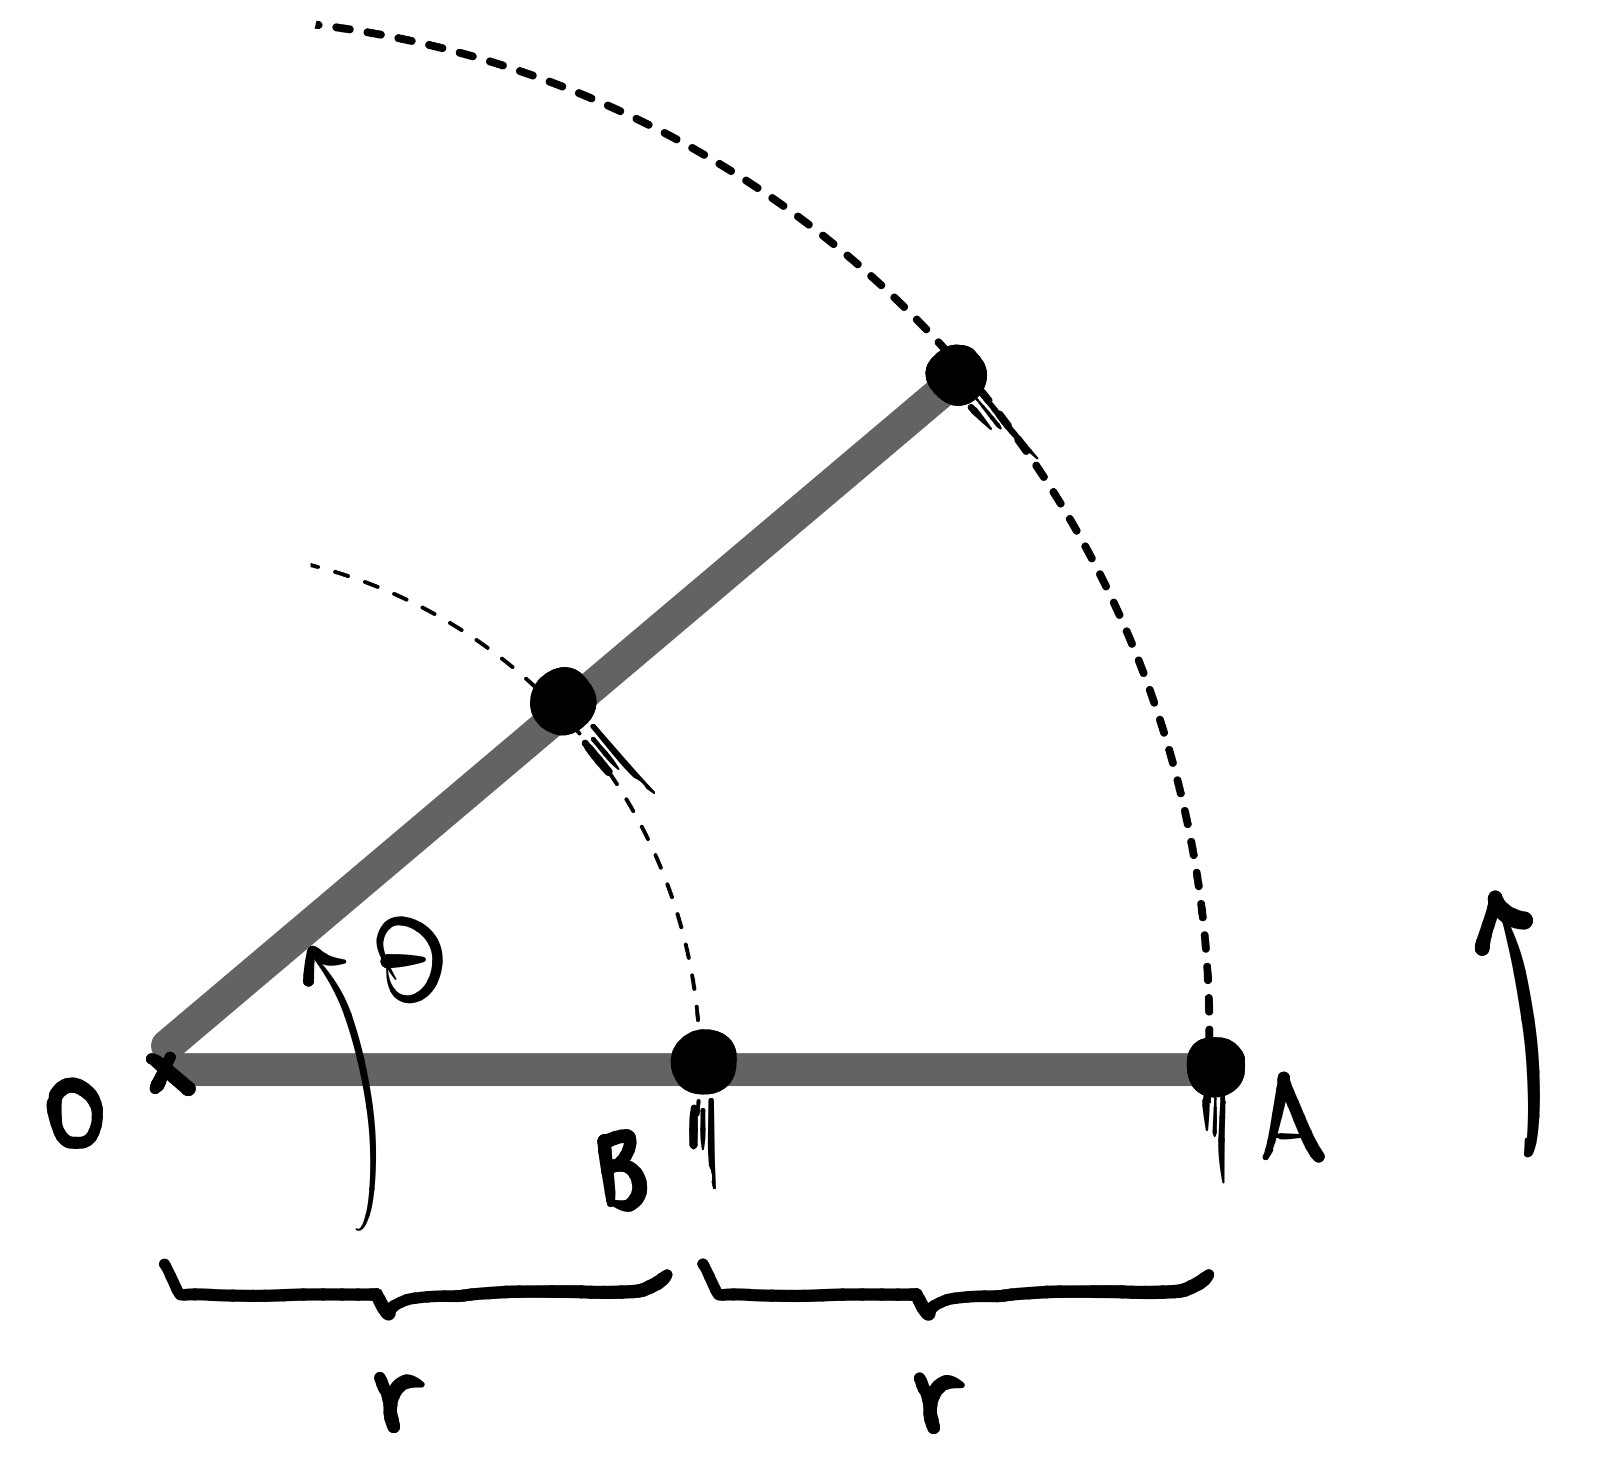
\includegraphics[width=0.35\linewidth]{imagenscinematicavetorial/v=wr exemplo01.png}
\captionof{figure}{}
\label{fig_cinvet_v=wr exemplo01}
} 

\vspace{0.3cm}

A figura tenta evidenciar isso, mostrando que, quando uma delas gira um certo ângulo $\theta,$ a outra, por estar fixa por uma haste rígida à primeira, obrigatoriamente gira, também, o mesmo ângulo. Logo, neste caso, podemos escrever que

$$ \omega_A = \omega_B \implies \dfrac{v_A}{R_A} = \dfrac{v_B}{R_B} \implies \dfrac{v_A}{2r} = \dfrac{v_B}{r} \implies \boxed{v_A = 2 v_B.}$$

Perceba que essa mesma conclusão poderia ter sido tirada sem o uso de equações: sendo o raio da circunferência $A$ o dobro do raio da circunferência $B,$ concluímos que o comprimento total da circunferência $A$ é o dobro do comprimento da circunferência $B.$ Logo, como as hastes giram juntas, quando $A$ completar uma volta, $B$ também terá completado uma volta, de modo que o período delas é o mesmo. Porém, tendo que varrer o dobro de distância no mesmo tempo, a velocidade linear de $A$ deve ser o dobro da de $B.$ \\

De certo modo, toda essa análise é capturada pelo tratamento matemático que fizemos ao usar $v = \omega r.$ Contudo, é importante entender o que se passa por trás dos processos algébricos ao manipular equações.

\end{exemplo}



\vspace{0.3cm}



\begin{exemplo}[Nível II]\label{exemplo_cinvet_velocidadeangularelinearex02}

Considere um ciclista que dá 2 pedaladas por segundo (cada pedalada significa realizar uma volta completa no disco acoplado aos pedais).

Se o raio do disco acoplado aos pedais é de 4cm, o raio da roda traseira é de 32 cm e o raio da catraca traseira -- que está acoplado por uma correia ao disco dos pedais -- é de 8 cm, qual é a velocidade com que o ciclista se move?

\resolucao

Sejam $A$, $B$ e $C$ o disco acoplado aos pedais, a catraca e a roda traseira, respectivamente. E sejam $R_A,$ $R_B,$ e $R_C$ os seus raios, respectivamente.


\vspace{0.3cm}
{
\centering
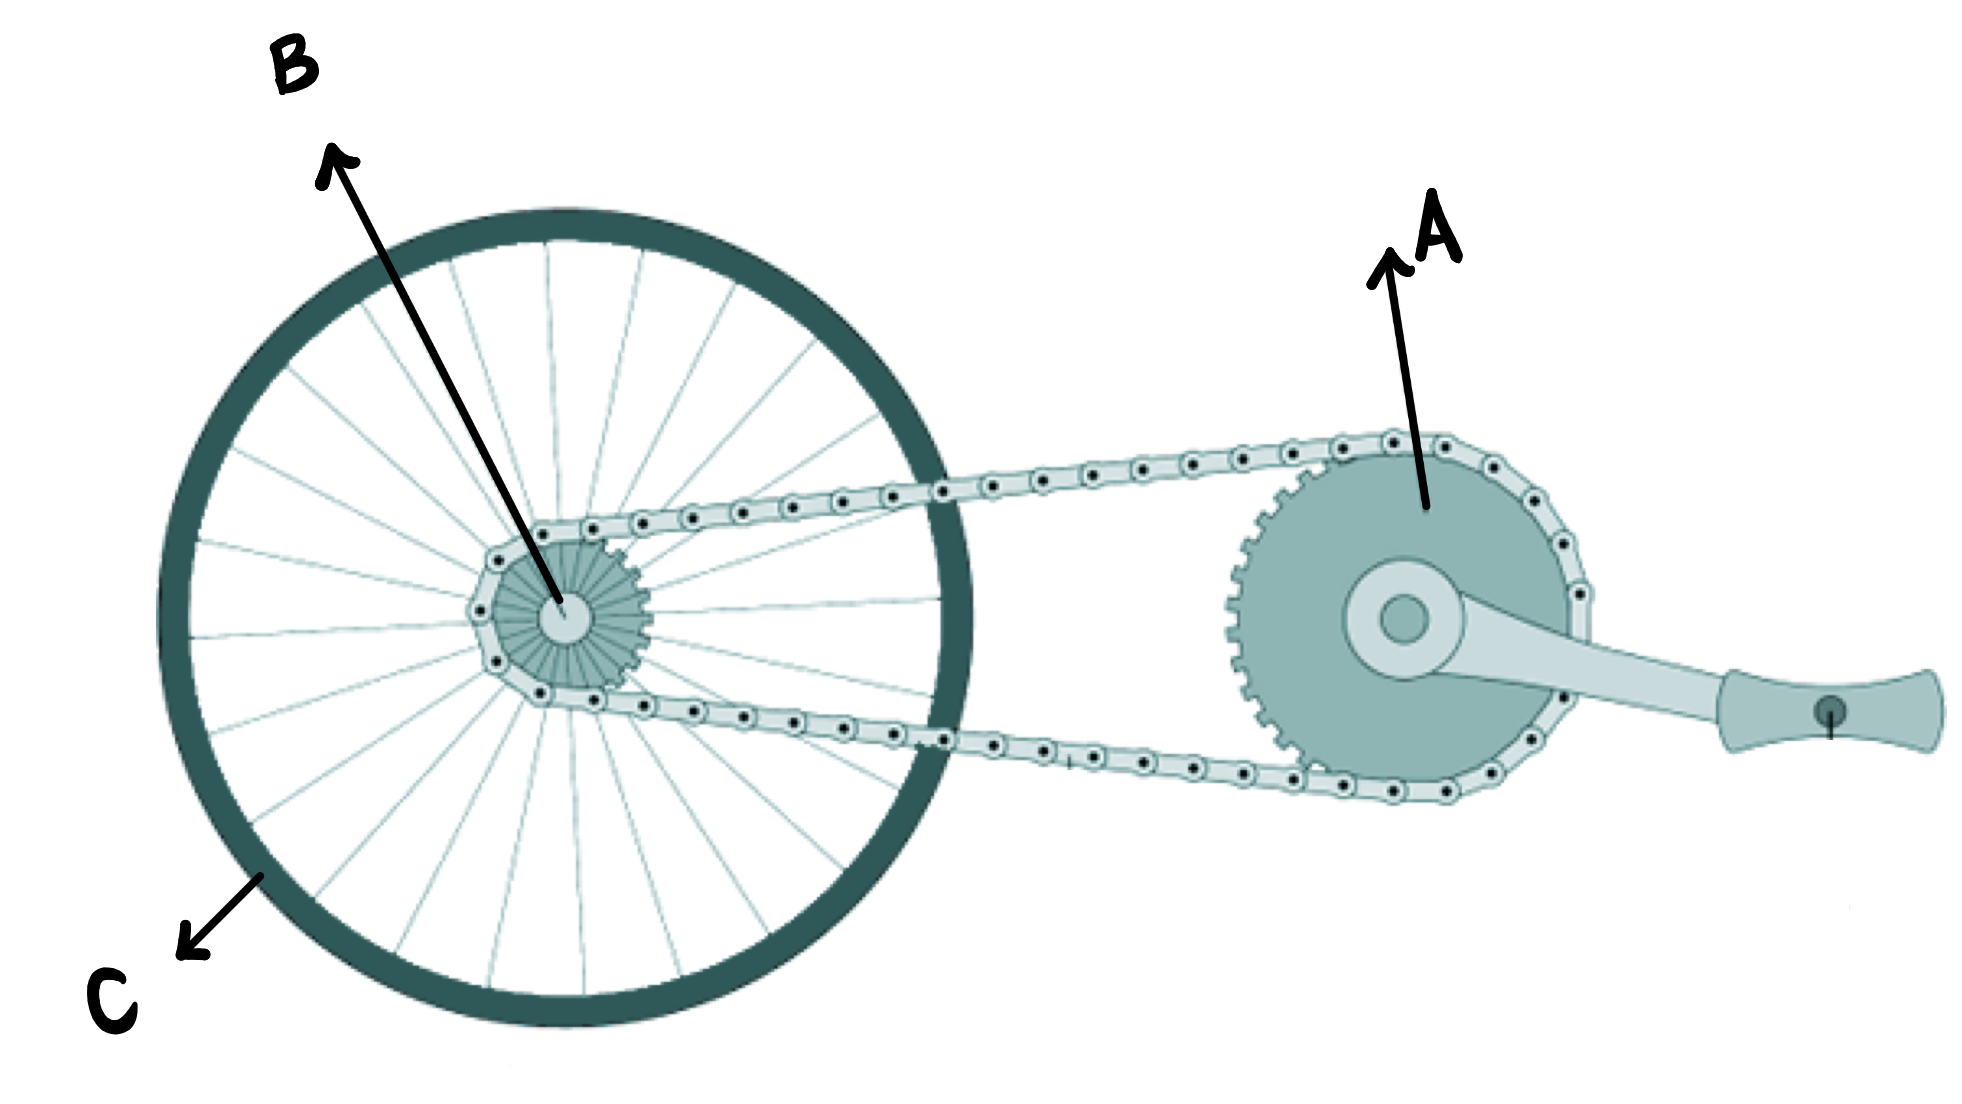
\includegraphics[width=0.5\linewidth]{imagenscinematicavetorial/bicicleta.png}
\captionof{figure}{}
\label{fig_cinvet_bicicelta}
} 

\vspace{0.3cm}


Como mostra Figura \ref{fig_cinvet_bicicelta}, a transmissão de movimento do disco acoplado aos pedais para a catraca se dá através de uma correia, que transmite a velocidade de um disco para o outro. Sendo a velocidade linear de todos os pontos da correia sempre a mesma, isso gera um acoplamento que obriga esses dois discos a girarem com mesma velocidade linear, ou seja:

$$ v_A = v_B \implies \omega_A R_A = \omega_BR_B \implies \omega_B = \omega_A\dfrac{R_A}{R_B}.$$


Já a catraca $B$ e a roda traseira $C$ giram sob um mesmo eixo, o que vem a ser o mesmo caso do exemplo anterior. Logo, elas possuem a mesma velocidade angular:

$$ \omega_B = \omega_C \implies  \omega_A \dfrac{R_A}{R_B} = \dfrac{v_C}{R_C} \implies v_C = \omega_A  \dfrac{R_A R_C}{R_B},$$

\noindent ou seja, para descobrir a velocidade da bicicleta $v_C$ -- que será igual à velocidade de movimento da sua roda traseira -- basta descobrir o valor da frequência angular $\omega_A$ de giro dos pedais. Ora, temos a informação de que o ciclista dá duas pedaladas por segundo, ou seja, o disco $A$ dá duas voltas por segundo: $f_A = 2$Hz. Logo, usando que $\omega = 2 \pi f,$ temos:

$$ \omega_A = 2 \pi f_A = 4 \pi \text{ Hz},$$

\noindent de modo que a velocidade $v_C$ da bicicleta é

$$ v_C = \omega_A  \dfrac{R_A R_C}{R_B} = 4 \pi \dfrac{0,04 \cdot 0,32}{0,08}  \approx 2 \text{ m/s.} $$

Note que convertemos os raios para metros, a fim de obter a resposta final em m/s.

\end{exemplo}




